\documentclass[12pt]{article}

\usepackage[margin=1in]{geometry}

\usepackage{fullpage}
%\usepackage[foot]{amsaddr}
\usepackage[utf8]{inputenc}
\usepackage[english]{babel}
\usepackage[shortlabels]{enumitem}
\usepackage{mathtools,
  booktabs,
  braket,
  mathrsfs,
  latexsym,
  epsfig,
  xcolor,
  url,
  setspace,
  graphics,
  lipsum,
  float,
  lineno,
  placeins
}
\usepackage{subfigure}
\usepackage{float}
\usepackage{pdflscape}
\newcommand{\bland}{\begin{landscape}}
\newcommand{\eland}{\end{landscape}}

% no indent for footnotes
\usepackage[flushmargin]{footmisc}
\setlength{\footnotemargin}{2mm}

\definecolor{CardinalRed}{cmyk}{0,1,0.65,0.34} % Cardinal Red
\usepackage[colorlinks,linkcolor=CardinalRed,citecolor=CardinalRed,urlcolor = CardinalRed]{hyperref}

\makeatletter
\def\maxwidth{\ifdim\Gin@nat@width>\linewidth\linewidth\else\Gin@nat@width\fi}
\def\maxheight{\ifdim\Gin@nat@height>\textheight\textheight\else\Gin@nat@height\fi}
\makeatother

% Scale images if necessary, so that they will not overflow the page
% margins by default, and it is still possible to overwrite the defaults
% using explicit options in \includegraphics[width, height, ...]{}
\setkeys{Gin}{width=\maxwidth,height=\maxheight,keepaspectratio}

\newcommand{\cred}[1]{\textcolor{CardinalRed}{#1}}
\newcommand{\red}[1]{\textcolor{red}{#1}}
\newcommand{\blue}[1]{\textcolor{blue}{(\bf{#1})}}
\newcommand{\burl}[1]{\textcolor{blue}{\url{#1}}}
\newcommand{\fix}[1]{\textcolor{red}{\textbf{ (#1)\normalsize}}}
\newcommand{\fixed}[1]{\textcolor{green}{~\\ \textbf{#1\normalsize}}\\}

%\renewcommand{\theequation}{\thesection.\arabic{equation}}
%\numberwithin{equation}{section}



% bibliography
\usepackage[round]{natbib}

\setcounter{secnumdepth}{5}

\setlength{\marginparwidth}{2cm}

\usepackage[OT1]{fontenc}

% \usepackage{mathpazo}
%\usepackage{fontspec}
% \setmainfont{TeX Gyre Pagella}
% \setcounter{secnumdepth}{0}

% \usepackage{todonotes}
\usepackage{todonotes}
% docs http://tug.ctan.org/macros/latex/contrib/todonotes/todonotes.pdf
% add todos using these steps
% \todo{margin comment}
% \todo[inline]{inline comment}
% \missingfigure{description of what should be in figure}

% this fixes incompatibility between todonotes and amsart [classic latex]
\makeatletter
\providecommand\@dotsep{5}
\def\listtodoname{List of Todos}
\def\listoftodos{\@starttoc{tdo}\listtodoname}
\makeatother

\graphicspath{{./graphs/}}%

% caption font
\usepackage[labelsep=period, font=sc, skip=0pt,justification=centering]{caption}
\usepackage[figuresright]{rotating}
% dot in section numbering
\usepackage{titlesec}
\titlelabel{\thetitle.\ }
%\startcontents[sections]

% no indent for thanks
\usepackage{titling}
\settowidth{\thanksmarkwidth}{*}
\setlength{\thanksmargin}{-\thanksmarkwidth}

% % reduce spacing for align environment
% \addtolength{\abovedisplayskip}{-2ex}
% \addtolength{\abovedisplayshortskip}{-2ex}
% \addtolength{\belowdisplayskip}{-2ex}
% \addtolength{\belowdisplayshortskip}{-2ex}

%% section head font size
\usepackage{titlesec}
\titleformat{\section}
{\normalfont\fontsize{15}{15}\bfseries}{\thesection.}{0.5em}{}

% spacing in itemizing
\newenvironment{itemize*}%
  {\begin{itemize}%
    \setlength{\itemsep}{0pt}%
    \setlength{\parskip}{0pt}}%
  {\end{itemize}}
\newenvironment{enumerate*}%
  {\begin{enumerate}%
    \setlength{\itemsep}{0pt}%
    \setlength{\parskip}{0pt}}%
  {\end{enumerate}}


% figure border
\renewcommand\fbox{\fcolorbox{blue}{white}}

% math packages
\usepackage{
  amscd,
  amsfonts,
  amsmath,
  amssymb,
  amsbsy,
  amsthm,
  bm, % boldmath
  dsfont,
  cancel, % cancellation
  latexsym,
  mathtools,
  graphicx,
  xcolor,
  xargs
}

% \usepackage[colorinlistoftodos,prependcaption,]{todonotes}

\usepackage{longtable}

\newcommand{\secend}{\vspace{3mm}}

\DeclareMathOperator{\erf}{erf}

\newcommand{\beq}{\begin{equation}}
\newcommand{\eeq}{\end{equation}}


% big parentheses
\newcommand*\Bigpar[1]{\left( #1 \right )}
\newcommand*\Bigbr[1]{\left[ #1 \right ]}
\newcommand*\Bigcr[1]{\left\{ #1 \right \}}
% set builder notation
\newcommand*\SetB[1]{\left\{ #1 \right\}}


% command shorthand
\newcommand{\eg}{e.g., \xspace}
\newcommand{\ie}{i.e.,\xspace}
\newcommand{\etc}{etc.\@\xspace}
\newcommand{\iid}{\emph{i.i.d.}\ }
\newcommand{\etal}{et.\ al.\ }
\newcommand{\wprob}{\text{w.p.}}
\newcommand{\D}{\displaystyle}
\newcommand{\ba}{\begin{array}}
\newcommand{\ea}{\end{array}}
\newcommand{\be}{\begin{enumerate}}
\newcommand{\ee}{\end{enumerate}}
\newcommand{\bi}{\begin{itemize}}
\newcommand{\ei}{\end{itemize}}
\newcommand{\bs}{\begin{align}\begin{split}\nonumber}
\newcommand{\bsnumber}{\begin{align}\begin{split}}
\newcommand{\es}{\end{split}\end{align}}
\newcommand{\fns}{\singlespace\footnotesize}

\def\ST{\text{\; s.t. \;}}
\def\WP{\text{\; w.p. \;}}
\def\IF{\text{\; if \;}}
\newcommand{\suchthat}{\text{ s.t. }}
\newcommand{\wrt}{\text{ w.r.t. }}
\providecommand{\subjectto}{\mathop{\rm subject\;to}}
\providecommand{\sto}{\mathop{\rm subject\;to}}
% ##     ##    ###    ######## ##     ##
% ###   ###   ## ##      ##    ##     ##
% #### ####  ##   ##     ##    ##     ##
% ## ### ## ##     ##    ##    #########
% ##     ## #########    ##    ##     ##
% ##     ## ##     ##    ##    ##     ##
% ##     ## ##     ##    ##    ##     ##


% derivative
% \newcommand{\deriv}[1]{\nabla \left{(#1 \right)}}

% \newcommandx\dbern[2][1=x,2=p]{#2^{#1} \left(1-#2\right)^{1-#1}}
\newcommandx{\deriv}[2][1=x,2=f]{\nabla \, #2 \Bigpar{ #1 } }

% Sums and products
\newcommand{\Sum}[2][i=1]{\ensuremath{\sum_{#1}^{#2}}}
\newcommand{\sumin}{\ensuremath{\sum_{i=1}^N}}
\newcommand{\sumiN}{\ensuremath{\sum_{i=1}^N}}
\newcommand{\sumim}{\ensuremath{\sum_{i=1}^m}}
\newcommand{\sumjk}{\ensuremath{\sum_{j=1}^k}}
\newcommand{\sumjj}{\ensuremath{\sum_{j=1}^J}}
\newcommand{\sumjn}{\ensuremath{\sum_{j=1}^n}}
\newcommand{\sumjm}{\ensuremath{\sum_{j=1}^m}}
\newcommand{\isum}[1][n]{\ensuremath{\sum_{#1}^\infty}}
\newcommand{\dsum}[4][i=1]{\ensuremath{\sum_{#1}^{#2}\sum_{#3}^{#4}}}
\newcommand{\Prod}[2][i=1]{\ensuremath{\prod_{#1}^{#2}}}
\newcommand{\prodin}{\ensuremath{\prod_{i=1}^N}}
\newcommand{\prodjn}{\ensuremath{\prod_{j=1}^n}}

% partial derivative
\newcommand{\dydx}[2]{\frac{\partial #1}{\partial #2}}
% vertical equal prefix
\newcommand{\verteq}{\rotatebox{90}{$\,=$}}
% vertical equal to
\newcommand{\equalto}[2]{\underset{\scriptstyle\overset{\mkern4mu\verteq}{#2}}{#1}}
% nullspace
\newcommand{\nulls}{\mathrm{null}}
% range
\newcommand{\range}{\mathrm{range}}

\newcommand*\maxx[1]{\text{max}\SetB{#1}}
\newcommand*\minn[1]{\text{min}\SetB{#1}}

% maximise
\newcommand{\maximise}{\operatornamewithlimits{max}}
\providecommand{\maximize}{\mathop{\rm maximize}}
% minimise
\newcommand{\minimise}{\operatornamewithlimits{min}}
\providecommand{\minimize}{\mathop{\rm minimize}}
% maximiser
\newcommand{\argmax}{\operatornamewithlimits{arg\,max}}
% general operator
\newcommand\oper[2]{\operatornamewithlimits{#1}_{#2}}


% indicator function
\newcommand*\Indic[1]{\mathds{1}_{#1}}

% ellipsis
\newcommand{\tto}{,\ldots,}

% blackboard F
\def\Function{\mathbb{F}}

% Lagrangian
\def\Lagr{\mathcal{L}}

% n-dimensional Real
\def\Realn{\mathbb{R}^n}

% k-dimensional Real
\def\Rk{\mathbb{R}^k}

% real with argument
\newcommand{\Realm}[1]{\mathbb{R}^{#1}}

% P_n
\def\Probn{\mathbb{P}_n}

\def\rel{\,{\buildrel R \over \sim}\,}
% generic m x n matrix
\newcommand{\gmatrix}[1]{\begin{bmatrix} {#1}_{11} & \cdots &{#1}_{1n} \\ \vdots & \ddots & \vdots \\ {#1}_{m1} & \cdots &{#1}_{mn} \end{bmatrix}}
% generic n x 1 vector
\newcommand{\gvec}[1]{\begin{bmatrix} {#1}_{1} \\ \vdots \\ {#1}_{n} \end{bmatrix}}

% matrix inverse
\newcommand{\inv}[1]{ \left({#1} \right)^{-1}}

% matrix transprose
\newcommand{\trap}[1]{ #1^{T}}

% 2 X 2 matrix
\newcommand{\mattwo}[4]
{\left(\begin{array}{cc}
                        #1  & #2   \\
                        #3 &  #4
                          \end{array}\right) }

\newcommand{\matthree}[9]
{\left(\begin{array}{ccc}
                        #1  & #2 & #3  \\
                        #4 &  #5 & #6 \\
                        #7 &  #8 & #9
                          \end{array}\right) }

\newcommand{\dettwo}[4]
{\left|\begin{array}{cc}
                        #1  & #2   \\
                        #3 &  #4
                          \end{array}\right| }

\newcommand{\detthree}[9]
{\left|\begin{array}{ccc}
                        #1  & #2 & #3  \\
                        #4 &  #5 & #6 \\
                        #7 &  #8 & #9
                          \end{array}\right| }



% inner product
\newcommand{\iprod}[1]{\left\langle {#1} \right\rangle}
% vector norm
\newcommand{\norm}[1]{\left\Vert{#1} \right\Vert}

% Trace
\newcommand{\trace}[1]{\text{tr} \left({#1} \right)}

% absolute value
\newcommand{\abs}[1]{\left\vert {#1} \right\vert}
% linalg misc
\renewcommand{\det}{\mathrm{det}}
\newcommand{\rank}{\mathrm{rank}}
\newcommand{\trc}{\mathrm{trace}}
\newcommand{\spn}{\mathrm{span}}
\newcommand{\row}{\mathrm{Row}}
\newcommand{\col}{\mathrm{Col}}
\renewcommand{\dim}{\mathrm{dim}}
% weakly prefer
\newcommand{\prefeq}{\succeq}
% strictly prefer
\newcommand{\pref}{\succ}
% sequence
\newcommand{\seq}[1]{\{{#1}_n \}_{n=1}^\infty }
% single arrow
\renewcommand{\to}{{\rightarrow}}
% double arrow
\newcommand{\corres}{\overrightarrow{\rightarrow}}
% evaluate at
\newcommand*\Eval[2]{\left.#1\right\rvert_{#2}}
% evaluate definite integral
\newcommand*\IntEval[3]{\left.#1\right\rvert_{#2}^{#3}}


%Blackboard Letters
\newcommand{\R}{\ensuremath{\mathbb{R}}}
\newcommand{\Z}{\ensuremath{\mathbb{Z}}}
\newcommand{\Q}{\mathbb{Q}}
\newcommand{\N}{\mathbb{N}}
\newcommand{\W}{\mathbb{W}}
\newcommand{\Qoft}{\mathbb{Q}(t)}  %use in linux

\newcommand\frakfamily{\usefont{U}{yfrak}{m}{n}}
\DeclareTextFontCommand{\textfrak}{\frakfamily}

% Fractions
\newcommand{\ooN}{\frac{1}{N}}  %oneforth
\newcommand{\fof}{\frac{1}{4}}  %oneforth
\newcommand{\foh}{\frac{1}{2}}  %onehalf
\newcommand{\fot}{\frac{1}{3}}  %onethird
\newcommand{\fop}{\frac{1}{\pi}}    %1/pi
\newcommand{\ftp}{\frac{2}{\pi}}    %2/pi
\newcommand{\fotp}{\frac{1}{2 \pi}} %1/2pi
\newcommand{\fotpi}{\frac{1}{2 \pi i}}
\newcommand{\cm}{c_{\text{{\rm mean}}}}
\newcommand{\cv}{c_{\text{{\rm variance}}}}

% minimiser
\newcommand{\argmin}{\operatornamewithlimits{arg\,min}}
% convergence in probability sideways
\def\inprobLOW{\rightarrow_p}
% convergence in probability
\def\inprobHIGH{\,{\buildrel p \over \rightarrow}\,}
% convergence in probability 2
\def\inprob{\,{\inprobHIGH}\,}
% convergence in distribution
\def\indist{\,{\buildrel d \over \rightarrow}\,}


% definition bench
\newcommand{\defeq}{\vcentcolon=}
\newcommand{\eqdef}{=\vcentcolon}

% blackboard F
\def\Function{\mathbb{F}}
% Natural
\def\Nat{\mathbb{N}}
% Integers
\def\Int{\mathbb{Z}}
% Reals
\def\Real{\mathbb{R}}
% Rationals
\def\Rat{\mathbb{Q}}
% Complex
\def\Cplx{\mathbb{C}}

% n-dimensional Real
\def\Realn{\mathbb{R}^n}
% expectation_n
\def\Expn{\mathbb{E}_n}
% P_n
\def\Probn{\mathbb{P}_n}
\def\rel{\,{\buildrel R \over \sim}\,}

\renewcommand{\det}{\mathrm{det}}
\renewcommand{\dim}{\mathrm{dim}}
% single arrow
\renewcommand{\to}{{\rightarrow}}

% generic vector and matrix
\newcommand{\mc}[1]{\mathcal{#1}}
\def\mbf#1{\mathbf{#1}}
\def\mrm#1{\mathrm{#1}}
\def\mbi#1{\boldsymbol{#1}} % Bold and italic (math bold italic)
\def\ve#1{\mbi{#1}} % Vector notation
\def\vea#1{\overrightarrow{#1}} % Vector notation

\newcommand*{\Vect}[1]{\mbi{#1}}
\newcommand*{\Mat}[1]{\mathbf{#1}}


\newcommand{\eucN}[1]{\norm{#1}} % l1 norm
\newcommand{\lzero}[1]{\norm{#1}_0} % l0 norm
\newcommand{\lone}[1]{\norm{#1}_1} % l1 norm
\newcommand{\ltwo}[1]{\norm{#1}_2} % l2 norm
\newcommand{\pnorm}[1]{\norm{#1}_p} % p-norm
\newcommand{\linf}[1]{\norm{#1}_\infty} % l-infinity norm
\newcommand{\lfro}[1]{\left\|{#1}\right\|_{\rm Fr}} % Frobenius norm
\newcommand{\matrixnorm}[1]{\left|\!\left|\!\left|{#1}
  \right|\!\right|\!\right|} % Matrix norm with three bars
\newcommand{\matrixnorms}[1]{|\!|\!|{#1}|\!|\!|} % Small matrix norm
\newcommand{\opnorm}[1]{\matrixnorm{#1}_{\rm op}}
\newcommand{\opnorms}[1]{\matrixnorms{#1}_{\rm op}}
\newcommand{\normbigg}[1]{\bigg\|{#1}\bigg\|} % A norm with 1 argument and bigg
                                              % brackets.
\newcommand{\lonebigg}[1]{\normbigg{#1}_1} % l1 norm
\newcommand{\ltwobigg}[1]{\normbigg{#1}_2} % l2 norm
\newcommand{\linfbigg}[1]{\normbigg{#1}_\infty} % l-infinity norm
\newcommand{\norms}[1]{\|{#1}\|} % A norm with 1 argument and normal (small)
                                 % brackets.
\newcommand{\lones}[1]{\norms{#1}_1} % l1 norm with small brackets
\newcommand{\ltwos}[1]{\norms{#1}_2} % l2 norm with small brackets
\newcommand{\linfs}[1]{\norms{#1}_\infty} % l-infinity norm with small brackets

\newcommand{\hinge}[1]{\left[{#1}\right]_+}

%%%%%%%%%%%%%%%%%%%%%%%%%%%%%%%%%%%%%%%%%%%%%%%%%%%%%%%%%%%%%%%%%%%%%
% tildes / hats / bars etc
%%%%%%%%%%%%%%%%%%%%%%%%%%%%%%%%%%%%%%%%%%%%%%%%%%%%%%%%%%%%%%%%%%%%%

\newcommand{\what}[1]{\widehat{#1}} % Wide hat
\newcommand{\wh}[1]{\widehat{#1}} % Wide hat
\newcommand{\wt}[1]{\widetilde{#1}} % Wide tilde
\newcommand{\wb}[1]{\overline{#1}} % Wide bar
% widehat, widetilde
\newcommand*\wtil[1]{\widetilde{#1}}
% over and underbars
\newcommand*\Ol[1]{\overline{#1}}
\newcommand*\Ul[1]{\underline{#1}}
% star
\newcommand*\Str[1]{#1^{*}}

\newcommand{\half}{\frac{1}{2}}

\newcommand{\<}{\left\langle} % Angle brackets
\renewcommand{\>}{\right\rangle} % End angle brackets

\renewcommand{\iff}{\Leftrightarrow}
\renewcommand{\choose}[2]{\binom{#1}{#2}}  % Choose
\newcommand{\chooses}[2]{{}_{#1}C_{#2}}  % Small choose

%%%% Probability symbols and associated distances %%%%

\newcommand{\E}{\mathbb{E}} % Expectation symbol
\renewcommand{\P}{\mathbb{P}} % Probability symbol
\newcommand{\var}{{\rm Var}} % Variance
\newcommand{\cov}{\mathop{\rm Cov}} % Covariance
\newcommand{\simiid}{\stackrel{\rm iid}{\sim}}
\newcommand{\openleft}[2]{\left({#1},{#2}\right]} % Interval open on left
\newcommand{\openright}[2]{\left[{#1},{#2}\right)} % Interval open on right

\newcommand{\indic}[1]{\mbf{1}\left\{#1\right\}} % Indicator function

% Distances between probability measures
\newcommand{\tvnorm}[1]{\norm{#1}_{\rm TV}} % Total variation
\newcommand{\tvnorms}[1]{\norms{#1}_{\rm TV}}
\newcommand{\dkl}[2]{D_{\rm kl}\left({#1} |\!| {#2}\right)} % KL divergence
\newcommand{\dkls}[2]{D_{\rm kl}({#1} |\!| {#2})}  % Small KL-divergence
\newcommand{\dchi}[2]{D_{\chi^2}\left({#1} |\!| {#2}\right)}  % chi^2-divergence
\newcommand{\fdiv}[2]{D_f\left({#1} |\!| {#2}\right)} % f divergence
\newcommand{\kl}[2]{D_{\rm kl}\left({#1} |\!| {#2} \right)}
\newcommand{\dhel}{d_{\rm hel}}  % Hellinger distance
\newcommand{\helaff}{A_{\rm hel}}  % Hellinger affinity



% Simple floor/ceiling stuff
\newcommand{\floor}[1]{\left\lfloor{#1} \right\rfloor}
\newcommand{\ceil}[1]{\left\lceil{#1} \right\rceil}

\providecommand{\argmax}{\mathop{\rm argmax}} % Defining math symbols
\providecommand{\argmin}{\mathop{\rm argmin}}
\providecommand{\soup}{\mathop{\rm sup}}

%  linalg stuff
\providecommand{\dom}{\mathop{\rm dom}}
\providecommand{\diag}{\mathop{\rm diag}}
\providecommand{\tr}{\mathop{\rm tr}}
\providecommand{\abs}{\mathop{\rm abs}}
\providecommand{\card}{\mathop{\rm card}}
\providecommand{\sign}{\mathop{\rm sign}}
\providecommand{\cl}{\mathop{\rm cl}}
\providecommand{\interior}{\mathop{\rm int}}
\providecommand{\conv}{\mathop{\rm Conv}}
\providecommand{\relint}{\mathop{\rm relint}}
\providecommand{\vol}{\mathop{\rm Vol}}
\providecommand{\supp}{\mathop{\rm supp}}


% Highlight part of eqn with colour
\newcommand*\hlred[1]{\textcolor{red}{#1}}
\newcommand*\hlblu[1]{\textcolor{blue}{#1}}


%  ######  ########    ###    ########  ######
% ##    ##    ##      ## ##      ##    ##    ##
% ##          ##     ##   ##     ##    ##
%  ######     ##    ##     ##    ##     ######
%       ##    ##    #########    ##          ##
% ##    ##    ##    ##     ##    ##    ##    ##
%  ######     ##    ##     ##    ##     ######


% data - curly D - Murphy notation
\def\Dat{\mathcal{D}}

% convergence in probability sideways
\def\inprobLOW{\rightarrow_p}
% convergence in probability
\def\inprobHIGH{\,{\buildrel p \over \rightarrow}\,}
% convergence in probability 2
\def\inprob{\,{\inprobHIGH}\,}
% convergence in distribution
\def\indist{\,{\buildrel d \over \rightarrow}\,}
% probability limit
\def\plim{\text{plim} \;}

% equality in distribution
\def\eqdist{\,{\buildrel d \over = }\,}

% independence (bench)
\newcommand\indep{\protect\mathpalette{\protect\independenT}{\perp}}
\def\independenT#1#2{\mathrel{\rlap{$#1#2$}\mkern5mu{#1#2}}}

% Likelihood
\newcommand{\Likl}{\mathcal{L}}
\newcommand{\Score}{\mathsf{S}}
\newcommand{\Hessian}{\mathsf{H}}

% bigO
\newcommand{\lilO}[1]{\mathsf{o}\Bigpar{#1}}
\newcommand{\bigO}[1]{\mathsf{O}\Bigpar{#1}}

% expectation
\newcommand{\Exp}[1]{\mathbb{E}\left[#1\right]}
% expectation at time
\newcommand{\Expt}[2]{\mathbb{E}_{#1}\left[#2\right]}
% expected utility for agent
\newcommand{\Expu}[1]{\mathbb{E}U^{#1}}
\newcommand{\Expua}[2]{\mathbb{E}U^{#1}\left[#2\right]}
\newcommand{\Expuat}[3]{\mathbb{E}U^{#1}_{#2}\left[#3\right]}
% variance
\newcommand{\Var}[1]{\mathbb{V}\left[#1\right]}
% covariance
\newcommand{\Covar}[1]{\text{Cov}(#1)}
% Probability
\newcommand{\Prob}[1]{\mathbf{Pr}\left(#1\right)}
% support
\newcommand{\Supp}[1]{\text{Supp}\left[#1\right]}

% generic estimators
\newcommand{\betahat}{\hat{\beta}}
\newcommand{\thetahat}{\hat{\theta}}

% CDF
\newcommand{\FF}{\mathbb{F}}
\newcommand{\ff}{\mathsf{f}}
\newcommand{\Cdf}[1]{\mathbb{F}\left(#1\right)}
\newcommand{\Cdff}[2]{\mathbb{F}_{#1}\left(#2\right)}
% PDF
\newcommand{\Pdf}[1]{\mathsf{f}\left(#1\right)}
\newcommand{\Pdff}[2]{\mathsf{f}_{#1}\left(#2\right)}

\newcommand{\F}{\mathbb{F}}


% Convergence of random variables
\newcommand{\cd}{\stackrel{d}{\rightarrow}}
\newcommand{\cas}{\stackrel{a.s.}{\rightarrow}}
\newcommand{\cp}{\stackrel{p}{\rightarrow}}

% Probability distributions
\newcommand*\normal[1]{\mathcal{N} \left( #1 \right )}
\newcommand*\Normal[1]{\mathcal{N} \left( #1 \right )}
% \newcommand{\unif}{\mathsf{U}}  % Uniform distribution
\newcommand*\Unif[1]{\mathsf{U} \left[ #1 \right ]}
\newcommand*\unif[1]{\mathsf{U} \left[ #1 \right ]}
% Bernoulli
\newcommand*\Bern[1]{\mathsf{Bernoulli} \left( #1 \right )}
\newcommand*\Binom[1]{\mathsf{Bin} \left( #1 \right )}
% Poisson
\newcommand*\Pois[1]{\mathsf{Poi} \left( #1 \right )}
% beta
\newcommand*\BetaD[1]{\mathsf{Beta} \left( #1 \right )}
% dirichlet
\newcommand*\Diri[1]{\mathsf{Dir} \left( #1 \right )}
% gamma
\newcommand*\Gdist[1]{\mathsf{Gamma} \left( #1 \right )}
% inv chi squared
\newcommand*\InvChi[1]{\mathsf{Inv}-\chi^2 \left( #1 \right )}

\def\bias{\textsf{bias}\xspace}
\def\se{\textsf{se}\xspace}
\def\pdf{\textsc{pdf}\xspace}
\def\cdf{\textsc{cdf}\xspace}
\def\ise{\textsc{ise}\xspace}
\def\pgf{\textsc{pgf}\xspace}
\def\mgf{\textsc{mgf}\xspace}
\def\mse{\textsc{mse}\xspace}
\def\mspe{\textsc{mspe}\xspace}
\def\mle{\textsc{mle}\xspace}
\def\mom{\textsc{mom}\xspace}
\def\are{\textsc{are}\xspace}
\def\rss{\textsc{rss}\xspace}
\def\ess{\textsc{ess}\xspace}
\def\tss{\textsc{tss}\xspace}


% Naming shortcuts.
\def\ahat{\ensuremath{\widehat{\alpha}}}
\def\atil{\ensuremath{\tilde{\alpha}}}
\def\bhat{\ensuremath{\widehat{\beta}}}
\def\btil{\ensuremath{\tilde{\beta}}}
\def\dhat{\ensuremath{\widehat{\delta}}}
\def\ehat{\ensuremath{\hat{\epsilon}}}
\def\ghat{\ensuremath{\widehat{\gamma}}}
\def\khat{\ensuremath{\widehat{\kappa}}}
\def\lhat{\ensuremath{\widehat{\lambda}}}
\def\ltil{\ensuremath{\tilde{\lambda}}}
\def\mhat{\ensuremath{\widehat{\mu}}}
\def\nhat{\ensuremath{\widehat{\nu}}}
\def\mtil{\ensuremath{\tilde{\mu}}}
\def\psihat{\ensuremath{\widehat{\psi}}}
\def\shat{\ensuremath{\widehat{\sigma}}}
\def\stil{\ensuremath{\tilde{\sigma}}}
\def\that{\ensuremath{\widehat{\theta}}}
\def\ttil{\ensuremath{\widetilde{\theta}}}
\def\rhohat{\widehat{\rho}}
\def\xihat{\widehat{\xi}}

\newcommand{\epsi}{\varepsilon}

\def\sehat{\ensuremath{\widehat{\se}}}
\def\fhat{\ensuremath{\widehat{f}}}
\def\Fhat{\ensuremath{\widehat{F}}}
\def\fnhat{\ensuremath{\widehat{f}_n}}
\def\Fnhat{\ensuremath{\widehat{F}_n}}
\def\Jhat{\ensuremath{\widehat{J}}}
\def\phat{\ensuremath{\widehat{p}}}
\def\ptil{\ensuremath{\tilde{p}}}
\def\rhat{\widehat{r}}
\def\Rbar{\bar{R}}
\def\Rhat{\widehat{R}}
\def\Qbar{\bar{Q}}
\def\Qhat{\widehat{Q}}
\def\Xhat{\widehat{X}}
\def\xbar{\bar{x}}
\def\Xbar{\bar{X}}
\def\Xsqbar{\overline{X^2}}
\def\xnbar{\overline{x}_n}
\def\Xnbar{\overline{X}_n}
\def\Yhat{\widehat{Y}}
\def\ybar{\overline{y}}
\def\Ybar{\overline{Y}}
\def\Ynbar{\overline{Y}_n}

% Random variables.
\def\rv{\textsc{rv}\xspace}
\def\iid{\ensuremath{\textsc{iid}}\xspace}
\def\dist{\ensuremath{\sim}\xspace}
\def\disteq{\ensuremath{\stackrel{D}{=}}\xspace}
\def\distiid{\ensuremath{\stackrel{iid}{\sim}}\xspace}
\def\ind{\ensuremath{\perp\!\!\!\perp}\xspace}
\def\nind{\ensuremath{\perp\!\!\!\!\big\vert\!\!\!\!\perp}\xspace}
\def\Xon{\ensuremath{X_1,\dots,X_n}\xspace}
\def\xon{\ensuremath{x_1,\dots,x_n}\xspace}
\def\giv{\ensuremath{\,|\,}}
\def\Giv{\ensuremath{\,\big|\,}}
\def\GIV{\ensuremath{\,\Big|\,}}
\newcommand{\indicator}[1]{\mathds{1}_{\left\{#1\right\}}}

% Probability, expectation, and variance.
\def\prob{\mathbb{P}}
\renewcommand{\Pr}[2][]{\ensuremath{\prob_{#1}\left[#2\right]}\xspace}
\newcommand{\V}[2][]{\ensuremath{\mathbb{V}_{#1}\left[#2\right]}}
\newcommand{\corr}[2][]{\ensuremath{\rho_{#1}\left[#2\right]}}
\def\sd{\ensuremath{\textsf{sd}}\xspace}
\def\samplemean{\ensuremath{\bar{X}_n}\xspace}
\def\samplevar{\ensuremath{S^2}\xspace}
\def\za{\ensuremath{z_{\alpha}}}
\def\zat{\ensuremath{z_{\alpha/2}}}

% Inference
\def\Ll{\ensuremath{\mathcal{L}}\xspace}
\def\Lln{\ensuremath{\Ll_n}\xspace}
\def\ll{\ensuremath{\ell}}
\def\lln{\ensuremath{\ll_n}}

% Hypothesis testing
\newcommand{\hyp}[2]{
\ensuremath{H_0:#1 \ifhmode\quad\text{versus}\quad\fi\text{ vs. } H_1:#2}}

% Convergence.
\def\conv{\rightarrow}
\def\convinf{\rightarrow_{n\to\infty}}
\def\pconv{\stackrel{\text{\tiny{P}}}{\rightarrow}}
\def\npconv{\stackrel{\text{\tiny{P}}}{\nrightarrow}}
\def\dconv{\stackrel{\text{\tiny{D}}}{\rightarrow}}
\def\ndconv{\stackrel{\text{\tiny{D}}}{\nrightarrow}}
\def\qmconv{\stackrel{\text{\tiny{qm}}}{\rightarrow}}
\def\nqmconv{\stackrel{\text{\tiny{qm}}}{\nrightarrow}}
\def\asconv{\stackrel{\text{\tiny{as}}}{\rightarrow}}
\def\nasconv{\stackrel{\text{\tiny{as}}}{\nrightarrow}}

%
% Distributions
%
\newcommandx{\uniff}[1][1={a,b}]{\textrm{Unif}\left({#1}\right)}
\newcommandx{\unifd}[1][1={a,\ldots,b}]{\textrm{Unif}\left\{{#1}\right\}}
\newcommandx{\dunif}[3][1=x,2=a,3=b]{\frac{I(#2<#1<#3)}{#3-#2}}
\newcommandx{\dunifd}[3][1=x,2=a,3=b]{\frac{I(#2\le#1\le#3)}{#3-#2+1}}
\newcommandx{\punif}[3][1=x,2=a,3=b]{
\begin{cases} 0 & #1 < #2 \\ \frac{#1-#2}{#3-#2} & #2 < #1 < #3 \\ 1 & #1 > #3\\\end{cases}}
\newcommandx{\punifd}[3][1=x,2=a,3=b]{
\begin{cases} 0 & #1 < #2\\ \frac{\lfloor#1\rfloor-#2+1}{#3-#2} & #2 \le #1 \le #3 \\ 1 & #1 > #3\\ \end{cases}}

% Bernoulli
\newcommandx\bern[1][1=p]{\textrm{Bern}\left({#1}\right)}
\newcommandx\dbern[2][1=x,2=p]{#2^{#1} \left(1-#2\right)^{1-#1}}
\newcommandx\pbern[2][1=x,2=p]{\left(1-#2\right)^{1-#1}}

% Binomial
\newcommandx\bin[1][1={n,p}]{\textrm{Bin}\left(#1\right)}
\newcommandx\dbin[3][1=x,2=n,3=p]{\binom{#2}{#1}#3^#1\left(1-#3\right)^{#2-#1}}

% Multinomial
\newcommandx\mult[1][1={n,p}]{\textrm{Mult}\left(#1\right)}
\newcommandx\dmult[3][1=x,2=n,3=p]{\frac{#2!}{#1_1!\ldots#1_k!}#3_1^{#1_1}\cdots#3_k^{#1_k}}

% Hypergeometric
\newcommandx\hyper[1][1={N,m,n}]{\textrm{Hyp}\left({#1}\right)}
\newcommandx\dhyper[4][1=x,2=N,3=m,4=n]{\frac{\binom{#3}{#1}\binom{#2-#3}{#4-#1}}{\binom{#2}{#4}}}

% Negative Binomial
\newcommandx\nbin[1][1={r,p}]{\textrm{NBin}\left({#1}\right)}
\newcommandx\dnbin[3][1=x,2=r,3=p]{\binom{#1+#2-1}{#2-1}#3^#2(1-#3)^#1}
\newcommandx\pnbin[3][1=x,2=r,3=p]{I_#3(#2,#1+1)}

% Geometric
\newcommandx\geo[1][1=p]{\textrm{Geo}\left(#1\right)}
\newcommandx\dgeo[2][1=x,2=p]{#2(1-#2)^{#1-1}}
\newcommandx\pgeo[2][1=x,2=p]{1-(1-#2)^#1}

% Poisson
\newcommandx\pois[1][1=\lambda]{\textrm{Po}\left({#1}\right)}
\newcommandx\dpois[2][1=x,2=\lambda]{\frac{#2^#1 e^{-#2}}{#1!}}
\newcommandx\ppois[2][1=x,2=\lambda]{e^{-#2}\sum_{i=0}^#1\frac{#2^i}{i!}}

% Normal
\newcommandx\normall[1][1={\mu,\sigma^2}]{\mathcal{N}\left({#1}\right)}
\newcommandx\dnormall[3][1=x,2=\mu,3=\sigma]%
  {\frac{1}{#3\sqrt{2\pi}}\exp \Bigpar{-\frac{\left(#1-#2\right)^2}{2 #3^2}}}
\newcommandx\pnormall[1][1=x]{\Phi\left({#1}\right)}
\newcommandx\qnormall[1]{\Phi^{-1}\left({#1}\right)}

% Multivariate Normal
\newcommandx\mvn[1][1={\mu,\Sigma}]{\mathrm{MVN}\left({#1}\right)}

% Exponential
\newcommandx\ex[1][1=\lambda]{\textrm{Exp}\left(#1\right)}
\newcommandx\dex[2][1=x,2=\lambda]{#2e^{-#1 #2}}
\newcommandx\pex[2][1=x,2=\lambda]{1-e^{-#1 #2}}

% Gamma
\newcommandx\gam[1][1={\alpha,\lambda}]{\textrm{Gamma}\left({#1}\right)}
\newcommandx\dgamma[3][1=x,2=\alpha,3=\lambda]%
  {\frac{#3^{#2}}{\Gamma\left( #2 \right)} #1^{#2-1}e^{-#3#1}}

% InverseGamma
\newcommandx\invgamma[1][1={\alpha,\beta}]{\textrm{InvGamma}\left({#1}\right)}
\newcommandx\dinvgamma[3][1=x,2=\alpha,3=\beta]%
{\frac{#3^{#2}}{\Gamma\left(#2\right)}#1^{-#2-1}e^{-#3/#1}}
\newcommandx\pinvgamma[3][1=x,2=\alpha,3=\beta]%
{\frac{\Gamma\left(#2,\frac{#3}{#1}\right)}{\Gamma\left(#2\right)}}

% Beta
\newcommandx\bet[1][1={\alpha,\beta}]{\textrm{Beta}\left(#1\right)}
\newcommandx\dbeta[3][1=x,2=\alpha,3=\beta]
{\frac{\Gamma\left(#2+#3\right)}{\Gamma\left(#2\right)\Gamma\left(#3\right)}#1^{#2-1}\left(1-#1\right)^{#3-1}}

% Dirichlet
\newcommandx\dir[1][1={\alpha}]{\textrm{Dir}\left(#1\right)}
\newcommandx\ddir[3][1=x,2=\alpha]{\frac{\Gamma\left(\sum_{i=1}^k #2_i\right)}{\prod_{i=1}^k\Gamma\left(#2_i\right)}\prod_{i=1}^k #1_i^{#2_i-1}}

% Weibull
\newcommandx\weibull[1][1={\alpha}]{\textrm{Dir}\left(#1\right)}
\newcommandx\dweibull[3][1=x,2=\lambda,3=k]{\frac{#3}{#2}
\left(\frac{#1}{#2}\right)^{#3-1} e^{-(#1/#2)^k}}

% Chi-squard
\newcommandx\chisq[1][1=k]{\chi_{#1}^2}

% Zeta
\newcommandx\zet[1][1=s]{\textrm{Zeta}\left(#1\right)}
\newcommandx\dzeta[2][1=x,2=s]{\frac{#1^{-#2}}{\zeta\left(#2\right)}}

% ######## ##    ## ##     ##  ######
% ##       ###   ## ##     ## ##    ##
% ##       ####  ## ##     ## ##
% ######   ## ## ## ##     ##  ######
% ##       ##  ####  ##   ##        ##
% ##       ##   ###   ## ##   ##    ##
% ######## ##    ##    ###     ######


% Proof environments
% The Theorems are numbered consecutively
% Lemmas are numbered by section, and observations, claims, facts, and
% assumptions take their numbering. Propositions and definitions have their
% own numbering by section.

% \theoremstyle{plain}

\newtheoremstyle{mystyle}%                % Name
  {}%                                     % Space above
  {}%                                     % Space below
  {}%                                     % Body font
  {}%                                     % Indent amount
  {\sffamily \bfseries }%                            % Theorem head font
  {.}%                                    % Punctuation after theorem head
  {\newline }%                                    % Space after theorem head, ' ', or \newline
  {\thmname{#1}\thmnumber{ #2}\thmnote{ (#3)}}%                                     % Theorem head spec (can be left empty, meaning `normal')


% \theoremstyle{definition}

\theoremstyle{mystyle}

\newtheorem{Theorem}{Theorem}[section]



\newtheorem{thm}{Theorem}[section]
\newtheorem{assum}{Assumption}
\newtheorem{defi}[Theorem]{Definition}
\newtheorem{cla}[thm]{Claim}
\newtheorem{conjecture}[thm]{Conjecture}
\newtheorem{conj}[thm]{Conjecture}
\newtheorem{cor}[thm]{Corollary}
\newtheorem{egg}[thm]{Example}
\newtheorem{exe}[thm]{Exercise}
\newtheorem{hypothesis}[thm]{Hypothesis}
\newtheorem{lem}[thm]{Lemma}
\newtheorem{proj}[thm]{Research Project}
\newtheorem{proposition}[thm]{Proposition}
\newtheorem{prop}[thm]{Proposition}
\newtheorem{que}[thm]{Question}
\newtheorem{rek}[thm]{Remark}
\newtheorem{rem}[thm]{Remark}
\newtheorem{fact}[thm]{Fact}
\newtheorem{propt}[thm]{Property}
\newtheorem{X}{X}[section]

\renewenvironment{proof}{\noindent{\bf Proof}\hspace*{1em}}{\qed\bigskip\\}
\newenvironment{proof-sketch}{\noindent{\bf Sketch of Proof}
  \hspace*{1em}}{\qed\bigskip\\}
\newenvironment{proof-idea}{\noindent{\bf Proof Idea}
  \hspace*{1em}}{\qed\bigskip\\}
\newenvironment{proof-of-lemma}[1][{}]{\noindent{\bf Proof of Lemma {#1}}
  \hspace*{1em}}{\qed\bigskip\\}
\newenvironment{proof-of-proposition}[1][{}]{\noindent{\bf
    Proof of Proposition {#1}}
  \hspace*{1em}}{\qed\bigskip\\}
\newenvironment{proof-of-theorem}[1][{}]{\noindent{\bf Proof of Theorem {#1}}
  \hspace*{1em}}{\qed\bigskip\\}
\newenvironment{inner-proof}{\noindent{\bf Proof}\hspace{1em}}{
  $\bigtriangledown$\medskip\\}
%% \newenvironment{proof-of-lemma}[1][{}]{\noindent{\bf Proof of Lemma {#1}}
%%   \hspace*{1em}\renewcommand{\qedsymbol}{$\bigtriangledown$}}{\qed\bigskip\\}
\newenvironment{proof-attempt}{\noindent{\bf Proof Attempt}
  \hspace*{1em}}{\qed\bigskip\\}
\newenvironment{proofof}[1]{\noindent{\bf Proof} of {#1}:
  \hspace*{1em}}{\qed\bigskip\\}
\newenvironment{remark}{\noindent{\bf Remark}
  \hspace*{1em}}{\bigskip}

% table alignment
\usepackage{array}
\newcolumntype{L}[1]{>{\raggedright\let\newline\\\arraybackslash\hspace{0pt}}m{#1}}
\newcolumntype{C}[1]{>{\centering\let\newline\\\arraybackslash\hspace{0pt}}m{#1}}
\newcolumntype{R}[1]{>{\raggedleft\let\newline\\\arraybackslash\hspace{0pt}}m{#1}}

% table multirow
\usepackage{multirow}

% expectation and probability
\def\e{\mrm{E}} % Expectation symbol
\def\E{\mathbb{E}} % Expectation symbol
\def\P{\mathbb{P}} % Probability symbol

% specifics to this paper
\def\Xit{X_{i,t}} 
\def\Ait{A_{i,t}} 
\def\Uit{U_{i,t}} 
\def\Yit{Y_{i,t}} 
\def\hYit{\hat{Y}_{i,t}} 
\def\Dit{D_{i,t}} 
\def\epit{\varepsilon_{i,t}} 
\def\Jit{J_{i,t}} 
\def\mcMit{\mc{M}_{i,t}} 

%\def\treatp{G_{i}}  % initial treatment time
\newcommand{\Ci}[1]{C_{i}^{(#1)}}%{Y_{#1}^{(g)}}


\def\Xigt{X_{i,g,t}}%^{(g)}} 
\def\Aigt{A_{i,g,t}}%^{(g)}} 
\def\Uigt{U_{i,g,t}}%^{(g)}} 
\def\Yigt{Y_{i,g,t}}%^{(g)}} 
\def\hYigt{\hat{Y}_{i,g,t}}%^{(g)}} 
\def\Digt{D_{i,g,t}}%^{(g)}}
\def\epigt{\epsilon_{i,g,t}}%^{(g)}}

\def\eventtime{E_{i,t}}%^{(g)}} 

\newcommand{\mYg}[1]{Y_{.,g,#1}}%{Y_{#1}^{(g)}}
\graphicspath{{./figure/}}%

%%%%%%%%%%%%%%%%%%%%%%%%%%%%%%%%%%%%%%%%%%%%%%%%%%%%%%%%%%
\begin{document}

%
%%%%%%%%%%%%%%%%%%%%%%%%%%%%%%%%%%%%%%%%%%%%%%%%%%%%%%%%%%

\title{\Large\bf What To Do (and Not to Do) with Causal Panel Analysis under  
Parallel Trends:\\Lessons from A Large Reanalysis Study%
\thanks{Albert Chiu, PhD student, Department of Political Science, Stanford University. Email: \url{altchiu@stanford.edu}. Xingchen Lan, PhD student, Wilf Family Department of Politics, New York University. Email: \url{xingchenlan@nyu.edu}. Ziyi Liu, PhD student, Haas School of Business, University of California, Berkeley. Email: \url{zyliu2023@berkeley.edu}. Yiqing Xu, Assistant Professor, Department of Political Science, Stanford University. Email: \url{yiqingxu@stanford.edu}. We thank Andrew Baker, Quintin Beazer, Kirill Borusyak, Kirk Bansak, Gary Cox, Avi Feller, Francisco Garfias, Justin Grimmer, Jens Hainmueller, Erin Hartman, Guido Imbens, Julia Payson, Annamaria Prati, Anton Strezhnev, Luwei Ying, participants at the 39th Political Methodology conference at Washington University in St. Louis, the 11th Asian Political Methodology Meeting at NYU Abu Dhabi, UCSD, and UC Berkeley, for helpful comments and suggestions. We thank Neil Malhotra and the Alethsia platform for providing pre-publication reviews of this paper. We are grateful to the authors of the articles we review for the constructive feedback and for making their data publicly available.}}


\author{Albert Chiu \\(Stanford)\and Xingchen Lan\\(NYU)\and Ziyi Liu\\(Berkeley)\and Yiqing Xu\\(Stanford)}

% \date{\small
%   First version: July 5, 2022\\
%   This version: 
%   \today
%   % \\ 
%   % {\small (Preliminary. Please do not circulate without permission.)}
%   \vspace{2em}
% }
\date{}

\maketitle

\vspace{-2em}
\begin{abstract}
\noindent Two-way fixed effects (TWFE) models are ubiquitous in causal panel analysis in political science. However, recent methodological discussions challenge their validity in the presence of heterogeneous treatment effects (HTE) and violations of the parallel trends assumption (PTA). This burgeoning literature has introduced multiple estimators and diagnostics, leading to confusion among empirical researchers on two fronts: the reliability of existing results based on TWFE models and the current best practices. To address these concerns, we examined, replicated, and reanalyzed 37 articles from three leading political science journals that employed observational panel data with binary treatments. Using six newly introduced HTE-robust estimators, along with diagnostics tests and uncertainty measures that are robust to PTA violations, we find that only a small minority of studies are highly robust. Although HTE-robust estimates tend to be broadly consistent with TWFE estimates, discrepancies in point estimates, increased measures of uncertainty, and potential PTA violations call into question many results that were already on the margins of statistical significance. We offer recommendations for improving practice in empirical research based on these findings.

\bigskip\noindent\textbf{Keywords:} panel data, two-way fixed effects, parallel trends,  heterogeneous treatment effects, pretrend, event-study plot, difference-in-differences, robust confidence set\vspace{2em}

%\bigskip\noindent\textbf{Word Count:} 9,982
\end{abstract}

\thispagestyle{empty}  % no page number for the first page
\clearpage
% \thispagestyle{empty}  % no page number for the first page
\newpage
\doublespace



\clearpage
%%%%%%%%%%%%%%%%%%%%%%%%

\setcounter{page}{1}


%%%%%%%%%%%%%%%%%%%%%%%%

\section{Introduction}

Over the past decade, political scientists have increasingly relied on observational panel data to draw causal conclusions \citep{Xu2023}. A favored method for such analyses is the two-way fixed effects (TWFE) model because of its ability to control for unobserved time-invariant characteristics of units and common time trends across units. In our survey of 90 articles published in three top political science journals from 2017 to 2022 using observational panel data with binary treatments, we find that 52 studies (58\%) employ the following canonical specification:\footnote{The remaining 38 articles can be categorized into five groups: articles focusing on interaction effects (8~articles), articles using nonlinear links such as logit and Poisson (5~articles), articles employing instrumental variables or regression discontinuity designs (8~articles), and articles using other linear specifications, such as only one-way fixed effects or lagged dependent variables (17 articles).}
\vspace{-0.5em}\begin{equation}\label{eq:twfe} 
  \Yit = \delta^{TWFE}\Dit + \Xit{'}\beta + \alpha_i + \xi_t + \epit, 
  \vspace{-0.5em}
\end{equation}
in which $\Yit$ is the outcome variable for unit $i$ at time $t$; $\Dit$ is the treatment variable; $\Xit$ is a vector of covariates; $\alpha_{i}$, $\xi_{t}$ are unit fixed effects and time fixed effects; and $\epit$ are idiosyncratic errors.\footnote{This is with some abuse of notation. In some articles that we classify as using TWFE models, ``unit'' fixed effects are at the level of ``groups'' $g$, within which multiple units $i$ are nested (e.g. county fixed effects when $i$ indexes city), or time fixed effects are at a higher level $p$ (e.g. year fixed effects when $t$ indexes day). While it would be more general and accurate to use the notation $\alpha_g$ and $\xi_p$, with $g=i$ and $p=t$ when fixed effects are at the finest-unit or -time level, we elect not to for the sake of simplicity.} The primary parameter of interest is $\delta^{TWFE}$, which researchers often interpret as the treatment effect. Moreover, researchers often equate TWFE models such as Model~(\ref{eq:twfe}) with difference-in-differences (DID) designs and use the two terms interchangeably.\footnote{We use the word ``design'' in reference to research design \citep{king2021designing}, which differs from the typical usage in the causal inference literature that refers to treatment assignment mechanism.}

Recent methodological discussions challenge the validity of TWFE models, leaving empirical researchers in a quandary. First, they do not know whether existing findings based on TWFE models are trustworthy. Second, with the introduction of numerous new estimators and diagnostics, researchers are uncertain about which estimator is most appropriate for their research context and what diagnostics they should employ. This paper seeks to bridge this gap by reviewing new diagnostic, estimation, and uncertainty quantification methods from the methodological literature and by reanalyzing published studies using both new estimators and the traditional TWFE model. Based on the findings, we offer recommendations for researchers.

Recent criticisms of the use of TWFE models mainly come from two directions. First, TWFE models require the \textit{strict exogeneity} assumption, which critics argue is stronger than many researchers realize and is often unrealistic in real-world settings \citep{Imai2019-nw}. Strict exogeneity implies the parallel trends assumption (PTA),
\vspace{-1em}\begin{equation}\label{eq:pta} \E[Y_{it} - Y_{it'}| {X}_{it},
X_{it'}] = \E[Y_{jt} - Y_{jt'}| X_{jt}, X_{jt'}]\quad \forall i, j, t, t',
\vspace{-1em}
\end{equation}
and threats to the PTA, such as the presence of time-varying confounders, anticipation effects, and feedback, also invalidate strict exogeneity. Therefore, in the rest of the paper, we refer to violations of strict exogeneity as violations of the PTA. 

The second group of criticism concerns the consequences of heterogeneous treatment effects (HTE) \citep[e.g.,][]{Goodman-Bacon2021-xb, CDH2020, Strezhnev2018-ku, Athey2018-re, callaway2021-did,BJS2021}. Researchers have shown that, under HTE, TWFE estimates in general do not converge to a convex combination of the individual treatment effects (ITE) for units under the treatment condition, even when the PTA is valid. The so-called ``negative weighting'' problem, as described in \citet{CDH2020}, is an extremely alarming theoretical result because it implies that a TWFE estimand can be negative (positive) even when all ITE are positive (negative). To address this issue, researchers have proposed many new estimators that are robust to HTE.

This paper thus pursues two goals. First, we explain and compare six recent proposals to amend TWFE models, including the interaction weighted (IW) estimator \citep{sun2021-event}, stacked DID \citep{BLW2022}, CS-DID \citep{Callaway2021-am}, DID multiple \citep{De_Chaisemartin2017-dk}, PanelMatch (\citealt{IKW2021}, hereafter IKW \citeyear{IKW2021}), and the imputation method (\citealt{BJS2021}, hereafter BJS \citeyear{BJS2021}; \citealt{LWX2022}, hereafter LWX \citeyear{LWX2022}). These estimators produce causally interpretable estimates under HTE and the PTA or its variants. Second, we replicate and reanalyze 37 studies published in the {\it American Political Science Review} (APSR), {\it American Journal of Political Science} (AJPS), and {\it The Journal of Politics} (JOP) from 2017 to 2022 whose main identification strategies rely on the PTA. Our aim is to assess the consequences of using or not using HTE-robust estimators and of potential PTA violations in political science research.

Our reanalysis shows that, although theoretically possible, HTE-robust estimators rarely result in complete reversals of conclusions based on the TWFE estimator in the political science literature. In fact, we observe only a single study where any of these estimators change the sign of the original finding, suggesting that the alarm over HTE generated by the theoretical literature may be out of proportion. The danger is instead more subtle: HTE-robust estimators tend to have larger measures of uncertainty, which, combined with even small fluctuations in point estimates, can undermine our confidence in a result. This is especially relevant for results that originally teeter on the brink of significance.  

Moreover, many studies either show clear signs of PTA violations or lack the power to dismiss the possibility that PTA violations of realistic sizes are responsible for a non-zero estimate of an average causal effect. In some studies, we observe signs of severe PTA violations, which likely have led to spurious findings. In others, allowing even mild violations of the PTA causes the original treatment effect estimates to become statistically indistinguishable from zero. This finding underscores how PTA violations persist and threaten the credibility of inferences drawn from observational panel data, despite being a longstanding and well-known assumption.

Overall, we find that about one-fourth to one-third of the articles in our sample present compelling empirical evidence to support their findings. These articles provide sufficient evidence that the PTA is plausible, and the statistically significant findings are robust under HTE and mild violations of the PTA benchmarked against observed ``pretrends,'' which are differences-in-means in the observed and predicted treated outcomes in the pretreatment periods. This does not imply that the remaining studies are incorrect; often, the available data do not permit detection or dismissal of PTA violations, nor do they allow us to reject the null hypothesis of no effects with sufficient power when using an HTE-robust estimator.

These findings have important implications for practice. First, whenever the PTA is invoked, it is essential for researchers to evaluate its plausibility using both graphical and statistical tools, as well as to consider the consequences of its potential violations through sensitivity analyses. Importantly, showing that coefficients of the ``pretrend'' are not statistically significantly different from zero does not suffice to validate the PTA. This is not only because the PTA involves counterfactuals and is inherently untestable, but also a classical case of equating ``absence of evidence'' as ``evidence of absence''---the lack of statistical significance could simply result from a lack of power. Second, we recommend that researchers favor HTE-robust estimators over TWFE. This is because the potential loss of efficiency, we believe, is justified by the reduction in risk of biases arising from HTE. We discuss the specific choice of estimator, which will depend on the research context and feasibility, in the Supplementary Materials (SM). 

In addition to offering researchers a set of practical recommendations, this paper makes several contributions. First, we propose a typology for and provide a comprehensive comparison of various estimators for causal panel analysis. We hope this discussion helps researchers deepen their understanding of these estimators. Ultimately, the validity of the identifying assumptions is more crucial than the choice of estimator, provided that the estimator is appropriate for the specific research context. Second, we adapt the robust confidence set (CS) approach for sensitivity analysis proposed by \citet{rambachan2023more} to the setting of counterfactual estimators. Third, our reanalysis both instills confidence in existing political science research conducted with TWFE models when done properly and raises warnings about potential risks, such as the failure of the PTA and a lack of power. Our work also contributes to the ongoing conversation on replication and reproducibility in political science \citep[e.g.,][]{eggers2015validity, lall2016multiple, hainmueller2019much,lal2021much}.


Our work is closely related to \citet{BLW2022}, who evaluate the credibility of a handful of studies with staggered adoption treatments in the finance and accounting literature. It differs from theirs in two important ways: (1) we apply a wider range of estimators and diagnostic tests to a much larger number of empirical applications from a more diverse selection of settings; his includes cases with treatment reversal, to which the majority of the studies we replicated belong. (2) This more comprehensive review suggests that the weighting problems caused by HTE may not be the primary threat to causal inference with panel data in political science research; instead, the primary concerns are PTA violations and a lack of statistical power. Our work is also related to \citet{roth2023s}, \citet{Xu2023}, and \citet{Arkhangelsky2023-zy}, who review and synthesize the recent methodological advancements of DID in the methodological literature. What differs is that we apply these innovations to empirical data, evaluate the robustness of existing findings, and provide practical advice to researchers. 


Our research has a few limitations. First, we do not explore methods that operate under sequential ignorability, an alternative identification framework that assumes no unobserved confounders but allows for dynamic treatment selection based on variables up to the current time period. Second, we do not address the challenge of cross-sectional interference, a phenomenon that is arguably prevalent in political and social settings. Third, although we point out how commonly the incorporation of lagged dependent variables (LDVs) or unit-specific linear time trends (ULTs) alters results in the SM, furthering the debate regarding whether or why these estimates should be trusted over the original ones is beyond the scope of this paper. Fourth, our analysis does not encompass studies that use continuous treatments, which is a common occurrence in political science research. Despite these limitations, which we aim to address in subsequent studies, our replication and reanalysis exercise provides valuable insights into some of the widespread and significant challenges in using TWFE models for panel data analysis.


%           $$\   $$\      $$$$$$\           $$\ $$\           
%           \__|  $$ |    $$  __$$\          $$ |$$ |          
%  $$$$$$\  $$\ $$$$$$\   $$ /  \__|$$$$$$\  $$ |$$ | $$$$$$$\ 
% $$  __$$\ $$ |\_$$  _|  $$$$\     \____$$\ $$ |$$ |$$  _____|
% $$ /  $$ |$$ |  $$ |    $$  _|    $$$$$$$ |$$ |$$ |\$$$$$$\  
% $$ |  $$ |$$ |  $$ |$$\ $$ |     $$  __$$ |$$ |$$ | \____$$\ 
% $$$$$$$  |$$ |  \$$$$  |$$ |     \$$$$$$$ |$$ |$$ |$$$$$$$  |
% $$  ____/ \__|   \____/ \__|      \_______|\__|\__|\_______/ 
% $$ |                                                         
% $$ |                                                         
% \__|                                                         
                                                             

\section{TWFE and Its Pitfalls} 

In this section, we review the pitfalls of TWFE models identified in the literature. In the classic two-group and two-period case, the OLS estimator (or equivalently, the least square dummy variable estimator) for the specification in Equation~(\ref{eq:twfe}), $\hat\delta^{TWFE}$, is equivalent to the DID estimator, which consistently estimates the average treatment effect on the treated (ATT) under the PTA even with HTE. These results do not hold more generally in more complex settings with differential treatment adoption times (known as staggered adoption) or treatment reversal, as we will discuss below.

Our survey of the top journals reveals that Model~(\ref{eq:twfe}) is the most commonly adopted approach for estimating causal effects using panel data in political science. Fixed effects (FE) models began their rise to prominence in political science in the early 2000s, and criticism promptly followed. 
For example, in a debate with
\citet{Green2001-dy}, \citet{Beck2001-as} and \citet{King2001-br} argue that
linear FE models often lead to misleading findings because they throw away
valuable information in data, ignore rich temporal dynamics, and are incapable
of capturing complex time-varying heterogeneities. Moreover, because both
the treatment and outcome variables are often serially correlated in a panel setting, researchers have cautioned against using standard error (SE) estimators suitable for cross-sectional data, such as Huber-White robust SEs \citep{Bertrand2004-rc}. Scholars have also advocated for bootstrap procedures to better control Type~I error rates when the number of clusters (units) is small \citep{Cameron2008-ou}.


In the past few years, a surge of studies has renewed investigation into the proprieties of the TWFE estimator and the assumptions it requires to achieve casual identification. One group of work studies TWFE models from a design-based perspective. For example, \citet{Imai2019-nw} point out that the \textit{strict
exogeneity} assumption required by TWFE models is stronger than researchers normally believe. Importantly, it not only implies the well-known no time-varying confounder requirement, but it also forbids a ``feedback'' effect from past outcomes to treatment assignment. \citet{Blackwell2018-br} clarify that such an assumption corresponds to baseline randomization in which the treatment vector is generated prior to, or independent of, the realization of the outcome. When knowledge about the treatment assignment mechanism is available, researchers have proposed design-based estimators to address unmeasured confounding of particular forms \citep[e.g.,][]{Arkhangelsky2019-zl, Arkhangelsky2021-ti}. Strict exogeneity or the PTA are the key identification assumptions of both the TWFE and the newer HTE-robust estimators that we discuss, but we find that in practice, a large number of studies in political science do not evaluate their plausibility. 


A second body of research explores the implications of HTE with binary treatments within TWFE models \citep[e.g.,][]{Goodman-Bacon2021-xb, CDH2020, Strezhnev2018-ku, callaway2021-did, BJS2021,Athey2018-re}. Most of this literature assumes staggered adoption, but the insights from that setting are still relevant when there are treatment reversals. In Figure~\ref{fg:toy}, we present two simplified examples with staggered treatment adoption. Figure~\ref{fg:toy}(a) represents outcome trajectories in line with standard TWFE assumptions, which not only include the PTA but also require that the treatment effect be immediate and unvarying across units and over time. In contrast, the right panel portrays a scenario where the PTA holds, but the constant treatment effect assumption is not met. Various decompositions by the aforementioned researchers reveal that even under the PTA, when treatments begin at different times (such as in staggered adoption) and treatment effects evolve over time, the TWFE estimand is not in general a convex combination of the ITE for observations subjected to the treatment. The basic intuition behind this theoretical result is that TWFE models use post-treatment data from units who adopt treatment earlier in the panel as controls for those who adopt the treatment later \citep[e.g.,][]{Goodman-Bacon2021-xb}. HTE-robust estimators capitalize on this insight by avoiding these ``invalid'' comparisons between two treated units in post-treatment periods. In the next section, we present a typology of HTE-robust estimators, along with an introduction to the estimators themselves.
% \footnote{The comparisons are valid if we are willing to assume constant treatment effects but not otherwise.}


\begin{figure}[!ht]
\caption{Toy Examples: TWFE Assumptions Satisfied vs. Violated}\label{fg:toy}
\vspace{-1em}
\centering
\begin{minipage}{1\linewidth}{
\centering
\hspace{0em}
\subfigure[Staggered DID: without Treatment Reversal]{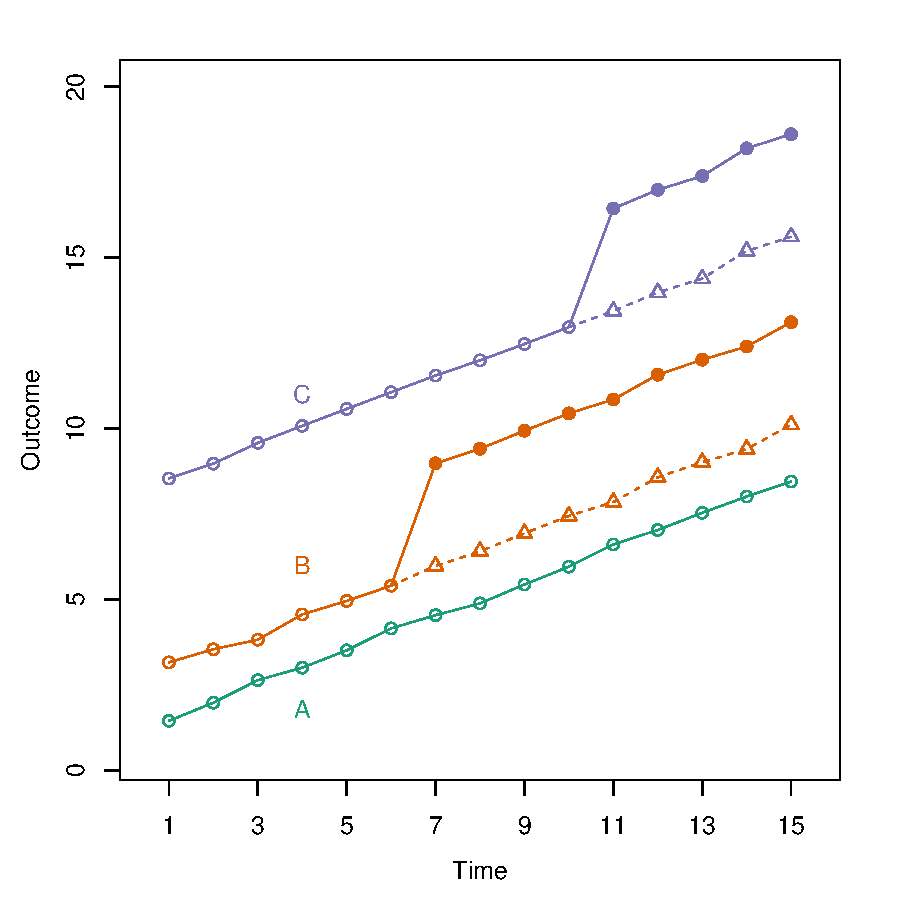
\includegraphics[width = 0.4\textwidth]{toy/toy_binary1a.pdf}\hspace{1em}
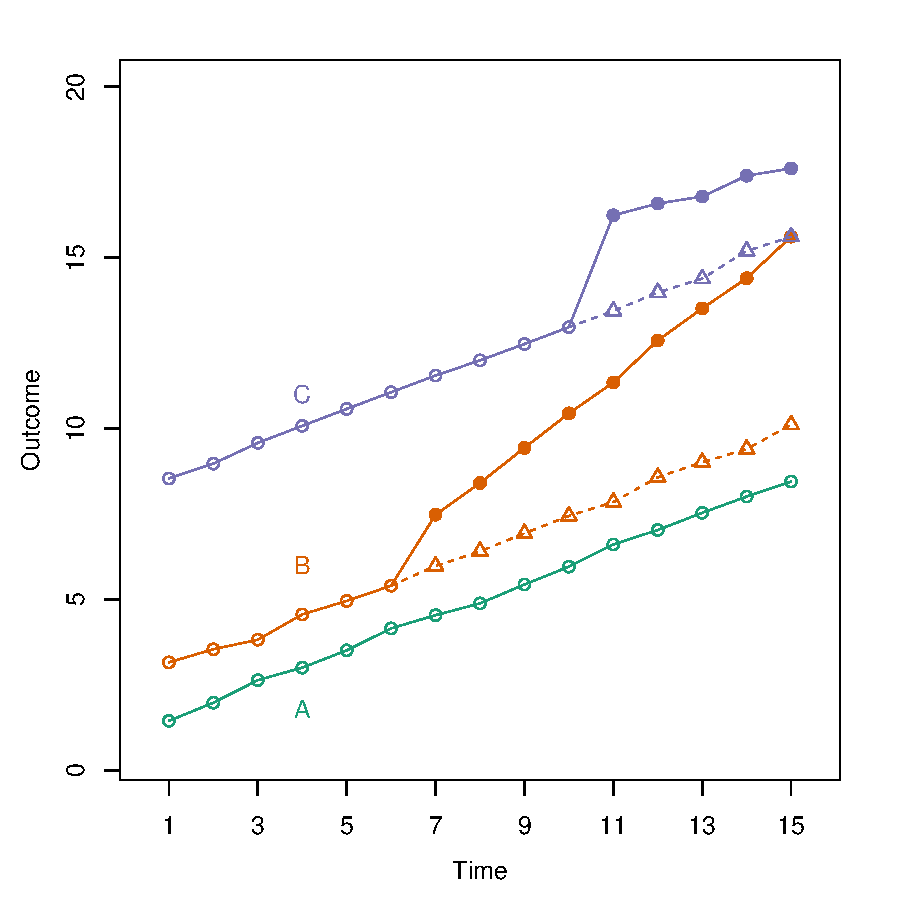
\includegraphics[width = 0.4\textwidth]{toy/toy_binary1b.pdf}}
\subfigure[Staggered DID: with Treatment Reversal]{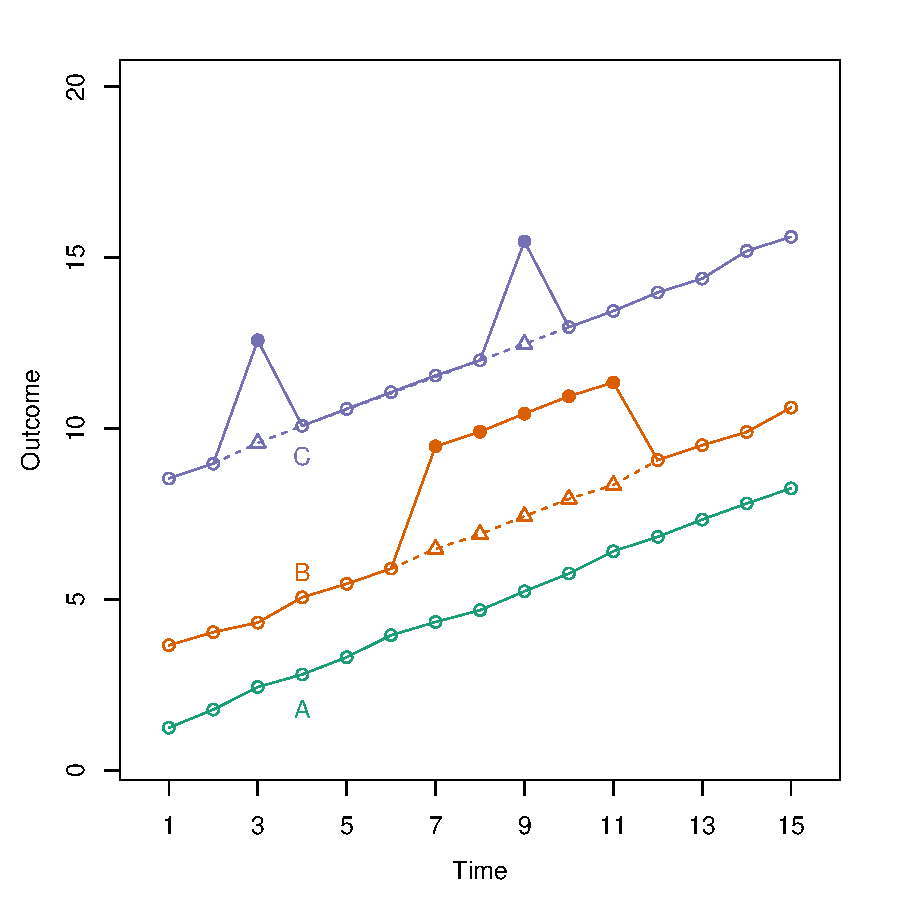
\includegraphics[width = 0.4\textwidth]{toy/toy_binary2a.pdf}\hspace{1em}
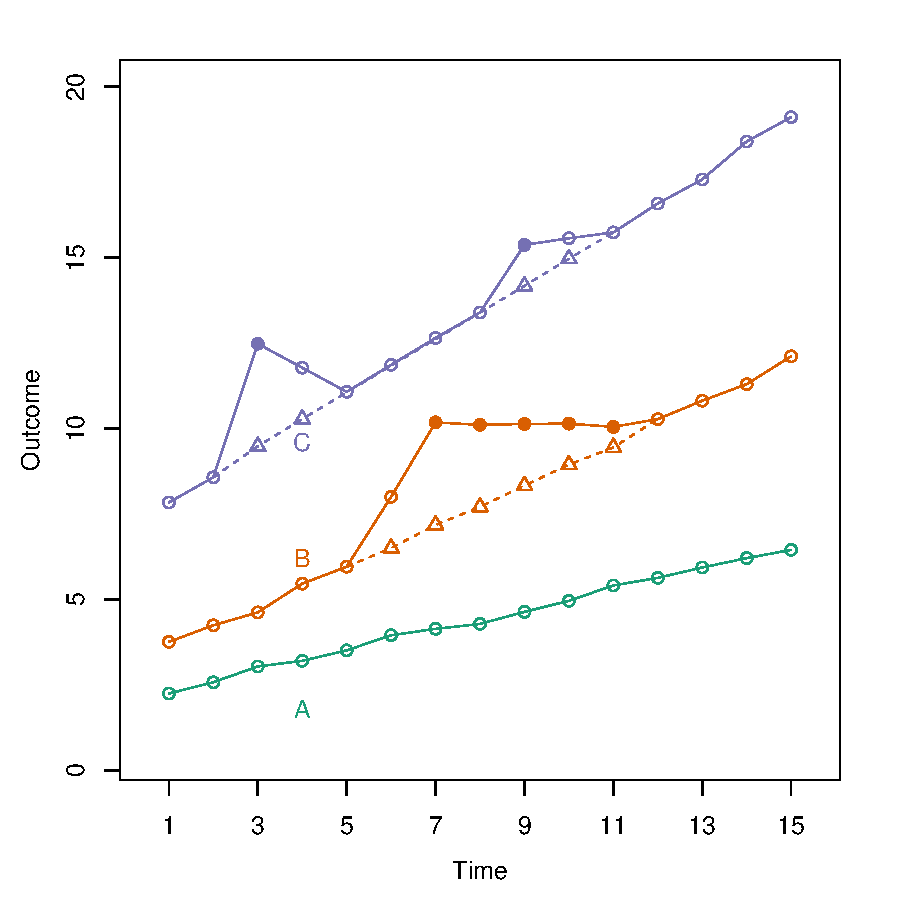
\includegraphics[width = 0.4\textwidth]{toy/toy_binary2b.pdf}}\\
}
\footnotesize\textbf{Note:} The above figures show outcome trajectories of units in a staggered adoption setting (a) and in a general setting (b). Solid and hollow circles represent observed outcomes under the treatment and control conditions, respectively, while triangles represent counterfactual outcomes (in the absence of the treatment). The data on the \emph{left} panels in both  (a) and (b) are generated by DGPs that satisfy TWFE assumptions while the data on the \emph{right} are not. The divergence between hollow circles and triangles in the right panel of (b), both of which are under the control condition, is caused by carryover effects. 
\end{minipage}\vspace{-0.5em}
\end{figure}

A third limitation of the canonical TWFE model is its presumption of no temporal and spatial interference. In most uses of TWFE models, researchers assume that there are no spatial spillovers and that treatment effects occur contemporaneously, hence no anticipation or carryover effects.\footnote{No anticipation effects means that future treatments do not affect today's potential outcomes; no carryover effects means that today's treatment does not affect future potential outcomes.} These are obviously strong assumptions that are rarely questioned or tested in practice \citep{Imai2019-nw, Athey2018-re, Wang2021-xo}. Although some recent methods permit arbitrary carryover effects in staggered adoption settings \citep{Strezhnev2018-ku, callaway2021-did}, they are not distinguishable from contemporaneous effects.\footnote{See Section A.4. of the SM in \citet{LWX2022} for more details.} This limitation becomes more complex when treatment reversal is possible, as demonstrated in Figure~\ref{fg:toy}. In Figure~\ref{fg:toy}(b), data in the left panel are consistent with TWFE assumptions, while the right panel shows deviations from the PTA, constant treatment effect, and the absence of anticipation or carryover effects. What is concerning is that many real-world data resemble the problematic right figure rather than the ideal left one. Nevertheless, recent methods have been proposed to handle arbitrary carryover effects over a limited number of periods in more general settings (IKW \citeyear{IKW2021}; LWX \citeyear{LWX2022}). The challenge of addressing spatial spillover effects without strong structural assumptions still persists \citep{Aronow2020-jc, Wang2021-xo}, but its resolution is beyond the scope of this paper.  

\paragraph*{Notation and Causal Estimands.} Consider the panel setting where multiple units $i\in\{1,\dots,N\}$ are observed at each time period $t\in\{1,\dots,T\}$. Each unit-time pair $(i,t)$ uniquely identifies an observation. 
For each $i$, let $\eventtime=\max\{t':t' \leq t, D_{i,t'}=1, D_{i,t'-1}=0\}$ for all $t$ such that $\exists s \leq t: D_{i,s}=1$ and $\eventtime=\min\{t':D_{i,t'}=1, D_{i,t'-1}=0\}$ otherwise. That is to say, $\eventtime$ is the most recent time at which unit $i$ switched into treatment or, if $i$ has not yet been treated at any point up until time $t$, the first time $i$ switches into treatment. If $i$ is never treated, we let $\eventtime=\infty$.
In the staggered setting, we call this the ``event time'' $E_i=\eventtime$, and
$\Dit=\indic{t \geq \eventtime}$, where $\indic{\cdot}$ is the indicator function. 
In a staggered adoption context, we partition units into distinct ``cohorts'' $g\in{1,\dots,G}$ according to the timing of treatment adoption $E_i$. Units transitioning to treatment at period $g$ ($i$ such that $\eventtime=g$) form cohort $g$, whereas units that never undergo treatment belong to the ``never-treated'' cohort ($i:\eventtime=\infty$). $Z_{i,t}$ ($Z_{i,g,t}$) represents the variable $Z$ for unit $i$ (part of cohort $g$) at time $t$. We use $\Yit(1)$ and $\Yit(0)$ to denote the potential outcomes under treatment and control, respectively, and $\Yit=\Dit \Yit(1) + (1-\Dit)\Yit(0)$ to denote the observed outcome.%
%
\footnote{The current notation will not cause confusion because we do not allow past outcome or covariates to affect current and future treatment status (no feedback). In some of the articles we refer to, potential outcomes are defined in
terms of treatment history, as opposed to current treatment status. We adopt
similar notations for these frameworks. For instance, we use $\Yit(\Dit~=~1,
\{D_{i,s}\}_{s<t}=0)$ to represent the potential outcome under the specified
treatment history. } %


The finest estimand is the ITE, $\tau_{i,t}=\Yit(1)-\Yit(0)$, of which there exists one for each observation $(i,t)$.%
%
\footnote{This is without loss of generality when feedback and interference are excluded. In staggered DID designs, carryover effects are permissible. When potential outcomes are defined in terms of treatment history, $\tau_{i,t}$ is defined as $\Yit(1)-\Yit(\infty)$ where $\Yit(\infty)$ signifies the untreated potential outcome when unit $i$ never undergoes treatment.} %
%
Most
political science research, however, typically focuses on estimating a single summary statistic. Commonly, this is the ATT, which represents ITE
averaged over all observations exposed to the treatment condition. 
In between these extremes of granularity and coarseness are time-varying dynamic treatment
effects (DTE), which are across-unit averages of ITE at each
time period relative to treatment adoption (e.g., all observations immediately proceeding treatment adoption). In the staggered adoption setting, we can further subdivide by cohort. We denote
the DTE $l$ periods after treatment adoption (for treatment cohort $g$) as
$\delta_{l}$ ($\delta_{g,l}$) and use $l=1$ to represent the period immediately after treatment adoption.%
\footnote{Some authors we reference to denote this first post-treatment period with $l=0$.} 
$\delta_{g,l}$ is also what some authors refer to as cohort average treatment effect on the treated (CATT) \citep{Strezhnev2018-ku, sun2021-event} or group-time average treatment effect \citep{callaway2021-did}.%



Each of the estimators we discuss can be used to estimate $\delta_l$. The specification analogous to TWFE for estimating DTE is a lags-and-leads specification. %A unit's treatment status
For simplicity, we first describe the staggered setting. Let $K_{i,t}=(t-\eventtime+1)$ be the number of periods until (when $K_{i,t}/leq 0$) or since unit $i$'s event time at time $t$ (e.g., $K_{i,t} = 1$ if unit $i$ switches into treatment at time $t$). Consider a regression based on the following specification:
\vspace{-1em}\begin{align}\label{eq:event-studies} 
\Yit = \alpha_i + \xi_t + X^{\prime}_{i,t}\beta + \sum_{\substack{l=-a\\l\neq 0}}^{b} \delta_{l}^{TWFE}
\cdot \indic{K_{i,t}=l} + \delta_{b+}^{TWFE}\indic{K_{i,t}> b}\cdot D_{i,t} + \epit, \vspace{-1em}
\end{align} 
where $a$ and $b$ are the number of lag and lead terms (BJS \citeyear{BJS2021}). In the social science literature, the typical practice is to exclude $l= 0$, which corresponds to the time period immediately before the transition into the treatment phase, and use it as a reference period \citep{roth2019pre}. Conventionally, $\hat\delta^{TWFE}_{l}$ is interpreted as an estimate of $\delta_l$ or as a meaningful weighted average of pertinent ITE. Meanwhile, $\hat\delta^{TWFE}_{b+}$ is viewed as an estimate for the long-term effect. We refer readers to Section A.4 in the SM for more information on Model~\eqref{eq:event-studies}, including in the case where there are treatment reversals.




%                       $$\     $$\                          $$\                                   
%                       $$ |    \__|                         $$ |                                  
%  $$$$$$\   $$$$$$$\ $$$$$$\   $$\ $$$$$$\$$$$\   $$$$$$\ $$$$$$\    $$$$$$\   $$$$$$\   $$$$$$$\ 
% $$  __$$\ $$  _____|\_$$  _|  $$ |$$  _$$  _$$\  \____$$\\_$$  _|  $$  __$$\ $$  __$$\ $$  _____|
% $$$$$$$$ |\$$$$$$\    $$ |    $$ |$$ / $$ / $$ | $$$$$$$ | $$ |    $$ /  $$ |$$ |  \__|\$$$$$$\  
% $$   ____| \____$$\   $$ |$$\ $$ |$$ | $$ | $$ |$$  __$$ | $$ |$$\ $$ |  $$ |$$ |       \____$$\ 
% \$$$$$$$\ $$$$$$$  |  \$$$$  |$$ |$$ | $$ | $$ |\$$$$$$$ | \$$$$  |\$$$$$$  |$$ |      $$$$$$$  |
%  \_______|\_______/    \____/ \__|\__| \__| \__| \_______|  \____/  \______/ \__|      \_______/ 
                                                                                                 
                                                                                                 
                                                                                                 
%%%%%%%%%%%%%%%%%%%%%%%%%%%%%%%%%%%%%%%%%
\section{HTE-Robust Estimators}\label{sc:methods}

In this section, we offer a brief overview and comparison of several recently introduced HTE-robust estimators. We use the term ``HTE'' to refer to ITE that are nonidentical, i.e. $\tau_{i,t} \neq \tau_{j,s}$ for some $i, j, s, t$,  and ``HTE-robust'' to refer to estimators that identify some convex combination of ITE even in the presence of HTE. For a more comprehensive discussion on all estimators mentioned in this section, please refer to the SM. 

\paragraph*{Summary of HTE-robust estimators.} Table~\ref{tb:estimators} summarizes the estimators we discuss in this paper. The primary difference resides in the mechanics of their estimation strategies: there are methods based on canonical DIDs and methods based on imputation. We refer
to the former as \emph{DID extensions} and the latter as \emph{imputation
methods}.\footnote{\citet{LSZ2022} use a similar dichotomy to describe these estimators.} DID extensions use DTE, estimated from local, $2\times2$ DIDs between treated and control observations, as building blocks. Imputation methods use ITE, estimated as the difference between an imputed outcome under control and the observed outcome (under treatment), as building blocks. Imputation methods connect to TWFE through the outcome model, which is fit globally on all available controls, that they use to impute counterfactual outcomes. Different strategies also entail different assumptions. Each DID extension, for example, relies on a particular type of PTA, whereas imputation methods presuppose a TWFE model for untreated potential outcomes and require a zero mean for the error terms.

Another noteworthy difference lies in the settings in which these estimators are applicable: some function exclusively in settings with staggered treatment adoption, while others can accommodate scenarios with treatment reversals.\footnote{It is possible to use some methods designed for the staggered setting even when there are reversals by using only a subset of the data, but this requires modifications to the original estimator and would identify a different effect than the ATT.} In the latter setting, all estimators we discuss also require a ``no carryover effects'' assumption, i.e., the treatment effect does not persist after the current period, regardless of which estimator is used and whether it is HTE-robust.
Furthermore, these estimators diverge in terms of (1) how they
select untreated observations as controls for treated units, (2) how
they incorporate pretreatment or exogenous covariates, and (3) the choice of
the reference period. We discuss these details further below and in Sections A.1. and A.4. of the SM.


\begin{table}[!ht]
    \centering
    \caption{Summary of HTE-Robust Estimators}\label{tb:estimators}
\resizebox{\textwidth}{!}{\small
\begin{tabular}{L{2.5cm} | C{2.5cm} C{2.5cm} C{2.5cm} | C{2.5cm} C{2.5cm} || C{2.6cm} C{2.5cm}}        \hline\hline
{\bf{Type}} & \multicolumn{5}{c||}{DID Extensions: uses $2\times 2$ DIDs as building blocks} & \multicolumn{2}{c}{Imputation Methods} \\ \hline
{\bf{Setting}} & \multicolumn{3}{C{7.5cm}|}{Staggered: treatment reversals not allowed} & \multicolumn{4}{c}{General: treatment reversals allowed} \\ \hline
{\bf{Research article}}    & \citet{sun2021-event} & \citet{callaway2021-did} & \citet{BLW2022} & \citet{CDH2020} & IKW \citeyearpar{IKW2021} & BJS \citeyearpar{BJS2021} & LWX \citeyearpar{LWX2022} \\ \hline
{\bf{Method known as}}  & \texttt{interaction weighted} & \texttt{csdid} & \texttt{StackedDID} & \texttt{did\_mulitple} & \texttt{PanelMatch} &  \texttt{DID$_{impute}$} & \texttt{FEct} \\ \hline
{\bf{Key ID assumption}}  & Parallel trends & Parallel trends & Parallel trends & Parallel
trends &  Parallel trends & Zero conditional mean & Strict exogeneity \\
\hline
{\bf{Finest estimand}}  & $\delta_{g,l}$ & $\delta_{g,l}$  & $\delta_l^{vw}$ & $\delta_{l}$ & $\delta_{l}$ &  $\tau_{i,t}$ & $\tau_{i,t}$ \\ \hline
{\bf{Comparison group}} & Never-treated or last-treated & Never-treated or 
not-yet-treated & Never-treated & Matched stable group (not-yet-treated) & Matched stable group
(not-yet-treated) & Imputed Counterfactual (not-yet-treated) & Imputed Counterfactual (not-yet-treated) \\ \hline
{\bf{Reference period(s)}} & Period 0 & An arbitrary pretreatment period & Period 0 & Untreated period & Period 0 & All pretreatment periods & All pretreatment periods \\ \hline
{\bf{Covariate adjustment}} & Possible extension & Outcome \& propensity score
modeling & Outcome modeling & Possible extension & Refined matched set \& outcome modeling & Outcome modeling &
Outcome modeling \\ \hline
\end{tabular}}
\end{table}


\paragraph*{DID extensions.} DID extensions are all built from local, $2 \times
2$ DID estimates---hence our choice of terminology. The overarching strategy for these estimators is to estimate the DTE, $\delta_{l}$ (or $\delta_{g,l}$ for each cohort $g$ in the staggered setting), for each period since the most recent initiation of treatment, $l$, using one or more \emph{valid} $2 \times 2$ DIDs. By ``valid,'' we mean that the DID includes (1) a pre-period and a post-period and (2) a treated group and a comparison group. The pre-period is such that all observations in both groups are in control, while the post-period is such that observations from the treated group are in treatment and those from the comparison group are in control. The choice of the comparison group is the primary distinction between estimators in this category. To obtain higher-level averages such as the ATT, we then average over our estimates of $\delta_{l}$ (or $\delta_{g,l}$), typically employing appropriate, convex weights.

We cover three estimators in this category that are appropriate only for the
staggered setting.  \citet{sun2021-event} propose an interaction-weighted
(\texttt{iw}) estimator, which is a weighted average of $\delta_{g,l}$ estimates obtained from a TWFE regression with cohort dummies fully interacted with indicators of relative time to the onset of treatment. They demonstrate that each resulting estimate of $\delta_{g,l}$ can be characterized as a difference in the change in average outcome from a fixed pre-period $s < g$ to a post-period $l$ periods since $g$ between the treated cohort $g$ and the comparison cohort(s) in some set $\mc{C}$.\footnote{This equivalence holds when the panel is balanced, i.e., there are no missing data. When there are missing data, the estimator from the saturated regression differs from one that directly estimates local DIDs, including the never-treated version of the next estimator we introduce, \texttt{csdid}.} The authors recommend using $\mc{C}={\sup_i E_i }$, which is either the never-treated cohort or, if no such cohort exists, the last-treated cohort. By default, \texttt{iw} uses $l=0$ as the reference period and can accommodate covariates in the TWFE regression. 

Employing the same general approach, \citet{callaway2021-did} propose two estimators, one of which uses never-treated units ($\hat\delta^{CS-dr}_{nev}$) and the other not-yet-treated units ($\hat\delta^{CS-dr}_{ny}$) as the comparison group. We label these estimators collectively as \texttt{csdid}. Note that $\hat\delta^{CS-dr}_{nev}$ uses the same comparison group as  \texttt{iw} when a never-treated cohort exists, whereas $\hat\delta^{CS-dr}_{ny}$ uses all untreated observations of not only never-treated units but also later adopters as controls for earlier adopters. Besides the choice of comparison cohort, \texttt{csdid} estimators differ from \texttt{iw} in that they allow users to condition on pretreatment covariates using both an explicit outcome model and inverse probability weighting (IPW) simultaneously, with at least one needing to be correct for the estimator to be consistent. While \texttt{iw} uses one period before the treatment's onset as the reference period, \texttt{csdid} allows users to choose one or multiple pretreatment periods as the reference.%
We will only implement $\hat\delta^{CS-dr}_{ny}$, as most models in our replication sample do not include additional covariates, rendering $\hat\delta^{CS-dr}_{nev}$ and $\hat\delta^{IW}$ numerically identical when there are no missing data.

The ``stacked'' DID or regression is another related estimator sometimes used to address HTE concerns. As described by \cite{BLW2022}, it involves creating separate sub-datasets for each treated cohort by combining data from that cohort (around treatment adoption) and never-treated cohort data from the same periods. These cohort-specific datasets are then ``stacked'' to form a single dataset. An event study regression akin to Equation~(\ref{eq:event-studies}) is then run, using sub-dataset specific unit and time dummies. This method is akin to \texttt{iw}  and the never-treated version of \texttt{csdid} without covariates; they all use the same data. However, stacked regression estimates a single DTE for a given relative period, rather than separate estimates for each cohort. Essentially, stacked DID is a special case of \texttt{iw} that uses immutable weights selected by OLS. We denote the corresponding estimand $\delta_l^{vw}$ to reflect the fact that it is variance-weighted. These weights will be convex, and so stacked DID avoids the ``negative weighting'' problem, but in general are not proportional to cohort sizes, and thus the stacked DID estimand is not the same as the ATT. This, however, is arguably a minor issue related to external validity, as the estimand will apply to a population with a different distribution over individual treatment effects (ITE).
% Stacked DID is not HTE-robust by our definition because OLS does not assign cohort-proportional weights; the effects for lower variance (larger) cohorts are generally down-weighted relative to their size. 

In settings with treatment reversals, separate groups of researchers have converged on the same strategy for choosing a comparison group: matching treated and control observations that belong to units with identical treatment histories. IKW~\citeyearpar{IKW2021} suggest one such estimator, \texttt{PanelMatch}, which begins by constructing a ``matched set'' for each pair $(i,t)$ such that unit $i$ transitions into treatment at time $t$. This matched set includes units that are both (1) not under treatment at time $t$ and (2) share the same treatment history as $i$ for a fixed number of periods leading up to the treatment onset. For each post-period $l$ periods since treatment adoption, it then estimates a local DID. It uses a fixed pre-period $s<t$ and the post-period $t-1+l$. The treatment ``group'' comprises solely of $(i,t)$, and the members of the matched set for $(i,t)$ that are still under control during that post-period serves as the comparison group. To obtain $\delta_l$ for a given $l$, it then averages over the relevant local estimates from all pairs $(i,t)$ such that $(i,t+l-1)$ is still under treatment (i.e., no treatment reversal has occurred yet). IKW~\citeyearpar{IKW2021} propose incorporating covariates by ``refining'' matched sets and use $l=0$ as the reference period.

Using a similar strategy, \citet{CDH2020} propose a ``multiple DID'' estimator, \texttt{DID$_M$}. A notable difference is that they include local DIDs for units leaving the treatment and not only those joining the treatment. The original proposal for \texttt{DID$_M$} also only considers the case where we match on a single period and where $l=1$.\footnote{The most recent version of the \texttt{DIDmultiplegt} allows for greater flexibility, bringing it closer in functionality to \texttt{PanelMatch}.} Consequently, the target estimand is not the ATT but rather an average of the contemporaneous effects of ``switching'' (i.e., the effect of joining or the negative of the effect of leaving at the time of doing so). Interestingly, another DID extension can be seen as a special case of \texttt{PanelMatch}: In the staggered setting, the \texttt{PanelMatch} estimator aligns with the not-yet-treated version of \texttt{csdid} (without covariate adjustment). We delve into details on the connections between these three estimators in Section A.1. of the SM.

All DID extensions are built using local, $2\times 2$ DIDs, and their assumptions reflect this. Specifically, they each rely on a form of the PTA, that is, the expected changes in non-treated potential outcomes from one period to the next are equal between the treated and the chosen comparison groups. In Table~\ref{tb:estimators}, we refer to all these assumptions collectively as the
PTA. We defer readers to the SM for a fuller account of each method's assumptions.


\paragraph*{The imputation method.} Imputation estimators do not explicitly estimate local DIDs. Instead, they take the difference between the observed outcome and an imputed counterfactual outcome for each treated observation. The connection to the TWFE model is in the functional form assumption used to impute counterfactual outcomes. Specifically, an imputation estimator first fits a parametric model for the potential outcome under control $\Yit(0)$---in our case, this is Model~(\ref{eq:twfe})---using only control observations $\{(i,t):\Dit=0\}$. It is also through this outcome model that one can adjust for covariates. Then, it imputes $\Yit(0)$ for all treated observations $\{(i,t):\Dit=1\}$ using the estimated parameters. Finally, it estimates the ITE, $\tau_{i,t}$, for each treated observation $(i,t)$ by calculating the difference between the observation's observed outcome $\Yit=\Yit(1)$ and its imputed counterfactual outcome $\hat{Y}_{i,t}(0)$. Inference for the estimated $\hat\tau_{i,t}$ is possible, although uncertainty estimates need to be adjusted to account for the presence of idiosyncratic errors \citep[e.g.,][]{bai2021matrix}.
BJS \citeyearpar{BJS2021} and LWX \citeyearpar{LWX2022} each propose estimators in this category. Each paper proposes a more general framework that nests many models, including TWFE. The latter also introduces several specific imputation estimators, one of which uses the TWFE model, and the authors refer to the resulting estimator as the fixed effect counterfactual estimator, or \texttt{FEct}.\footnote{BJS \citeyearpar{BJS2021} and LWX \citeyearpar{LWX2022} estimate pretreatment DTE in event-study plots differently. The former uses the first period as reference, while the latter uses the average of all pretreatment periods. We prefer the latter method in DTE estimation because the former may produce event-study plots that are visually counterintutitive \citep{Roth2024interpret}.} 


Compared to DID extensions, which typically use a single pre-period and, with
the exception of \texttt{csdid}, only a subset of units under control at both the pre- and post-periods as a comparison group, imputation estimators use all available control observations to estimate treated counterfactuals. As such, for each unit, the reference period can be understood as (the average of) all pretreatment periods. Intuitively, this approach should result in higher efficiency. In fact, BJS \citeyearpar{BJS2021} demonstrate that imputation estimators are the most efficient among all estimators under the condition of homoskedastic errors. Also in contrast to DID extensions, imputation estimators do not directly assume the PTA. Instead, they restrict the expectation of the error terms from a parametric TWFE model. In Table 2, this is denoted as ``zero conditional mean'' for BSJ \citeyearpar{BJS2021} or ``strict exogeneity'' for LWX \citeyearpar{LWX2022}. Again, we refer readers to the SM for the formal statements of these assumptions. Collectively, these assumptions imply a form of conditional, baseline randomization of treatment assignment, which in turn implies the PTA \citep[e.g.,][]{Blackwell2018-br}.



Although DID extensions and imputation methods rely on slightly different identification assumptions, such as the PTA and specific constraints on the error terms, they usually lead to similar observable implications. Researchers commonly use the presence or absence of pretrends to judge the plausibility of the PTA. In the classic two-group, two-period setting, if there are data from additional pretreatment periods, researchers can plot the time series of (average) outcomes of each group and visually inspect whether they indeed trend together. The intuition is that if the PTA holds and the outcome trends of the treated and control groups are indeed parallel in pretreatment periods when $Y(0)$'s are observed for all units, then it is plausible that the PTA also holds in the post-treatment periods, when $Y(0)$'s are no longer observable for units in the treatment group. Conversely, differential trends in the pretreatment periods should make us suspicious of the PTA. In more complex settings or where we wish to control for observed confounders, researchers often use estimates of the dynamic effects before and after the onset of treatment, $\delta_l$, to construct so-called ``event-study plots'' to judge the presence of pretrends. If the PTA holds, then pretreatment DTE estimates should be around zero. We provide a more thorough discussion and examples of the event-study plots in the next section when we introduce our procedure. 




%%%%%%%%%%%%%%%%%%%%%%%%%%%%%%%%%%%%%%%%%


\FloatBarrier

% $$$$$$$\             $$\               
% $$  __$$\            $$ |              
% $$ |  $$ | $$$$$$\ $$$$$$\    $$$$$$\  
% $$ |  $$ | \____$$\\_$$  _|   \____$$\ 
% $$ |  $$ | $$$$$$$ | $$ |     $$$$$$$ |
% $$ |  $$ |$$  __$$ | $$ |$$\ $$  __$$ |
% $$$$$$$  |\$$$$$$$ | \$$$$  |\$$$$$$$ |
% \_______/  \_______|  \____/  \_______|

                                       
\section{Data and Procedure}\label{sc:data}

Next, we assess the robustness of empirical findings from causal panel analyses in
political science and compare results obtained using the different methods we have discussed. We will explain our sample selection rules, describe standard practices in the field, and outline our reanalysis approach. Readers can find a more detailed explanation of our sample selection criteria and replication and reanalysis procedure in Sections A.3. and A.4. of the SM.

\paragraph*{Data.} Our replication sample comprises articles from three leading
political science journals---the {\it APSR}, {\it AJPS}, and {\it JOP}---published over a recent six-year span from 2017 to 2022. We initially include all studies, including both long and short articles, that employ panel data analyses with a binary treatment as a crucial component of their causal argument, resulting in a total of 90 articles. After a careful review of each of these articles, we find that 52 articles use a TWFE model similar to Model~(\ref{eq:twfe}). We then attempt to replicate the main results of these 52 articles and are successful in 37 cases (71.2\%). Though a significant proportion of papers failed to replicate, we note that the success rate is still higher than that of \citet{hainmueller2019much} at 55\% and is comparable to that of \citet{lal2021much}, which stands at 67\%. We credit this to the new replicability standards set by journals. A detailed explanation of how we select the ``main model'' is provided in Section A.3. of the SM. Table~\ref{tb:replicability} depicts the distribution of successful replications, along with reasons for replication failures, across the various journals.

\begin{table}[!htbp]
  \centering\small
   \caption{Sample Selection and Replicability of Qualified Articles}
    \label{tb:replicability}
   \begin{tabular}{C{1.8cm}C{1.7cm}C{2.2cm}cccc}\hline\hline\small
      &      & TWFE & Incomplete & Replication &  &  Success\\
    Journal  & All &  (attempted)  &  data    &  error  &   Replicable & Rate\% \\\hline
    {\it APSR} &  18 & 9    & 2     & 1     & 6     & 66.7 \\
    {\it AJPS} &  28 & 18    & 3     & 3     & 12     & 66.7 \\
    {\it JOP}  &  44 & 25    & 6     & 0     & 19    & 76.0 \\ \hline
    Total      & 90 & 52    & 11    & 4     & 37    & 71.2 \\\hline
    \end{tabular}%
\end{table}\vspace*{-1em}


 
\paragraph*{Settings and common practices.} Table~\ref{tb:practice} presents an overview of the standard practices and settings in the articles that we successfully replicated. The vast majority of studies in our sample (92\%) use DID designs to justify the use of the TWFE model, while the remaining studies advocate for the model's ability to exploit ``within'' variations in the data. Out of the 37 articles, five (13\%) employ a classic DID design, which includes two-group, two-period designs (three articles) and multi-period DID designs (two articles). 10 articles (27\%) use a staggered (but not classic) DID design, while the remaining 22 articles (59.5\%) fall into the ``general'' category, meaning they allow for treatment reversals. Except for four articles, all studies have a continuous outcome of interest. Most studies adopt cluster-robust SEs or panel-corrected SEs \citep{Beck1995-am}, while five articles apply bootstrap procedures for estimating uncertainties. A subset of authors explore alternative model specifications by adding LDVs (six articles), ULTs (11 articles) and higher-than-unit-level time trends (5 articles). Notably, 22 studies use some type of plot---either average outcomes over time, event-study plots, or both---to evaluate the plausibility of the PTA. 

\begin{table}[!htbp]
  \centering\small
  \caption{Settings and Common Practice}\label{tb:practice}%
    \begin{tabular}{lccclcc}\hline\hline
        \textbf{Motivations for TWFE} &       &       &  &  \textbf{Variance Estimator}   &  &        \\ 
        ``Difference-in-differences" & 34     & 92\% &  &     Cluster-robust SE or PCSE & 36    & 97.3\%  \\
    ``Within" variations & 3     & 8\% &  &     Cluster-bootstrapped procedures & 5     & 13.5\%    \\
          &       &       &  &  \\
    \textbf{Treatment Setting} &       &       &  &  \textbf{Variants in specifications}   &  &        \\ 
    Classic 2$\times$2 DID & 3     & 8.1\% &       &  LDVs  & 6     & 16.2\%  \\
    Classic multi-period DID & 2     & 5.4\% &       & Higher-than-unit-level time trends & 5 & 13.5\% \\
    Staggered DID & 10    & 27\% &       & ULTs & 11     & 29.7\%  \\
    General & 22    & 59.5\% &       &    \\ 
          &       &       &  &                       \textbf{Data visualization}   \\
    \textbf{Outcome Variable} & &    &   & Group average outcomes & 14    & 37.8\%     \\ 
    Continuous  &  33   &  89.2\%     &    &  event-study plots & 18    & 48.6\%   \\ 
    Binary  &   4    &   11.8\%    &         & Neither   &  15  & 40.5\% \\ \hline
\end{tabular}%
\end{table}\vspace{-1em}%




\FloatBarrier

% $$$$$$$\                                                $$\                               
% $$  __$$\                                               $$ |                              
% $$ |  $$ | $$$$$$\   $$$$$$\   $$$$$$$\  $$$$$$\   $$$$$$$ |$$\   $$\  $$$$$$\   $$$$$$\  
% $$$$$$$  |$$  __$$\ $$  __$$\ $$  _____|$$  __$$\ $$  __$$ |$$ |  $$ |$$  __$$\ $$  __$$\ 
% $$  ____/ $$ |  \__|$$ /  $$ |$$ /      $$$$$$$$ |$$ /  $$ |$$ |  $$ |$$ |  \__|$$$$$$$$ |
% $$ |      $$ |      $$ |  $$ |$$ |      $$   ____|$$ |  $$ |$$ |  $$ |$$ |      $$   ____|
% $$ |      $$ |      \$$$$$$  |\$$$$$$$\ \$$$$$$$\ \$$$$$$$ |\$$$$$$  |$$ |      \$$$$$$$\ 
% \__|      \__|       \______/  \_______| \_______| \_______| \______/ \__|       \_______|
                                                                                          

\paragraph*{Procedure.} We use data from \citet{Grumbach2020} to illustrate our process for replication and reanalysis. The study investigates the influence of coethnic mobilization by minority candidates during US congressional elections.
To simplify our analysis, we focus on the impact of the presence of an Asian candidate on the proportion of general election contributions from Asian donors.  

To begin, we aim to understand the research setting and data structure. We visualize the patterns of treatment and outcome variables using plots, which are shown in the SM. In this application, treatment reversals clearly take place. Some data is missing (due to redistricting), but the issue does not seem to be severe. We record important details such as the number of observations, units, and time periods, the type of variance estimator, and other specifics of the main model (not shown here). Next, we replicate the main finding, employing both the original variance estimator and a cluster-bootstrap procedure. We also use a bootstrap refinement procedure recommended by \citet{Cameron2008-ou} to conduct statistical testing; the results are broadly consistent with the ones based on cluster-bootstrapped SEs and CIs.  %

We then re-estimate the ATT and DTEs using estimators discussed in Section~\ref{sc:methods}. For staggered adoption treatment cases, we apply six estimators: TWFE (with always treated units removed for easier comparisons with other estimators), \texttt{PanelMatch}, the imputation estimator \texttt{FEct}, Stacked DID, \texttt{iw}, and \texttt{csdid} (not-yet-treated). For applications with treatment reversals like \citet{Grumbach2020}, we use the first three estimators only. The comparison between the TWFE estimate and the other estimates sheds light on whether original findings are sensitive to the presence of HTE. Figures~\ref{fg:gs2020}(a)-(d) show the results from this example. The similarity between estimates for ATTs in (a) suggests that the original finding is robust to the choice of estimators. The event-study plots from HTE-robust estimators in (c)-(d) are broadly consistent with the event-study plot from TWFE in (b).


\begin{figure}[!ht]
  \caption{Reanalysis of \citet{Grumbach2020}}\label{fg:gs2020}
  \centering
  \begin{minipage}{1\linewidth}{
  \begin{center}
  \hspace{-1em}
  \subfigure[Treatment effect estimates]{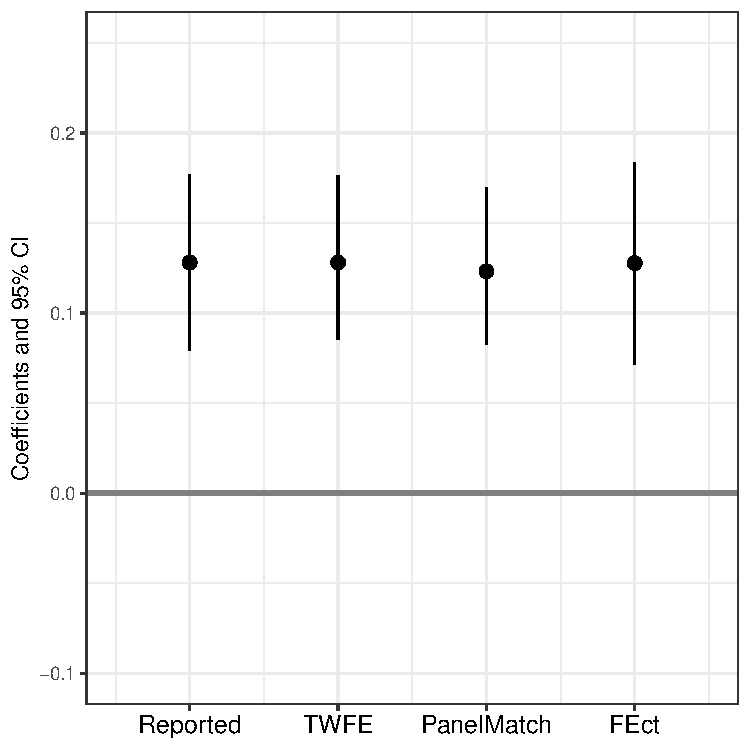
\includegraphics[width = 0.28\textwidth]{apps/gs2020_compare.pdf}}\hspace{1em}
  \subfigure[DTE: TWFE]{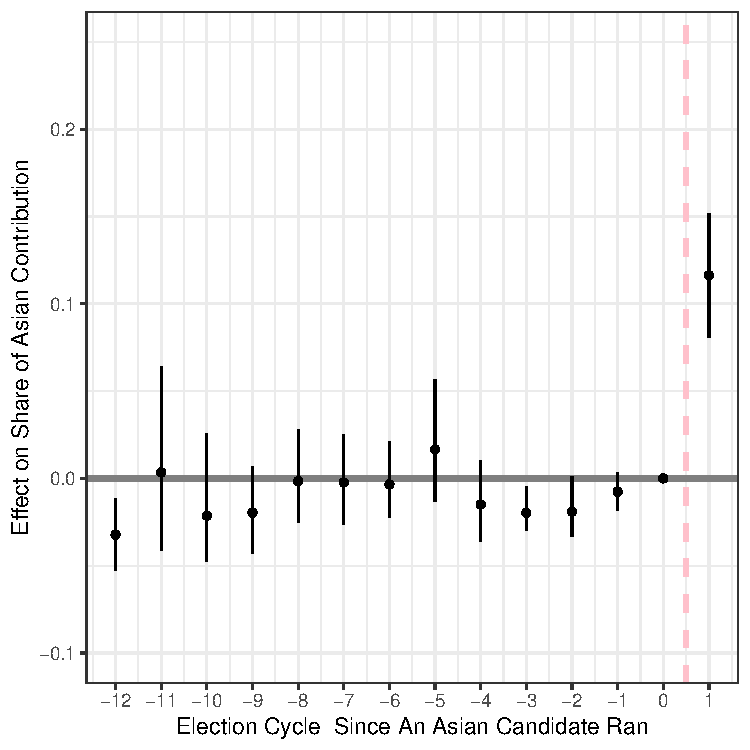
\includegraphics[width = 0.28\textwidth]{apps/gs2020_twfe.pdf}}\hspace{1em}
  \subfigure[DTE: \texttt{PanelMatch}]{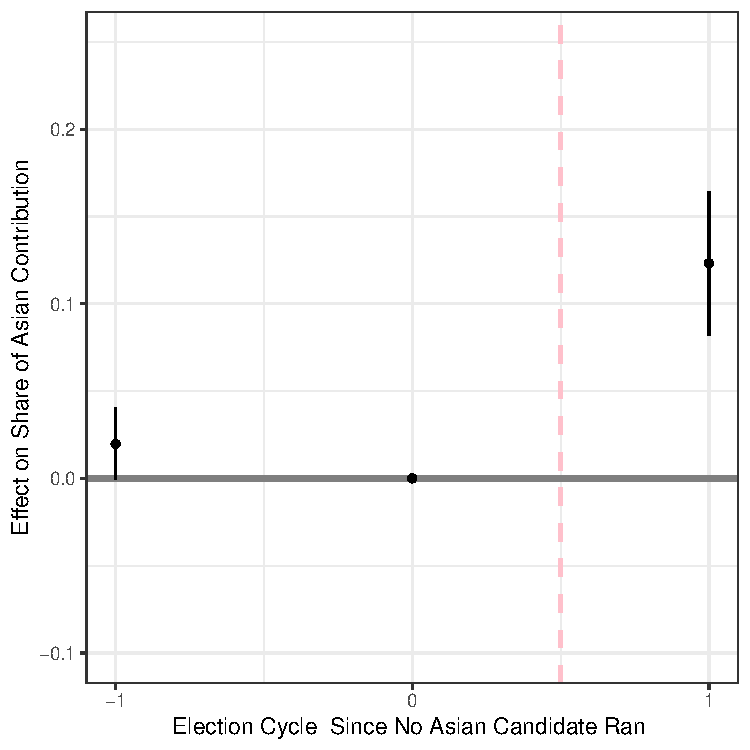
\includegraphics[width = 0.28\textwidth]{apps/gs2020_pmatch.pdf}}\\
  \subfigure[DTE: \texttt{FEct}]{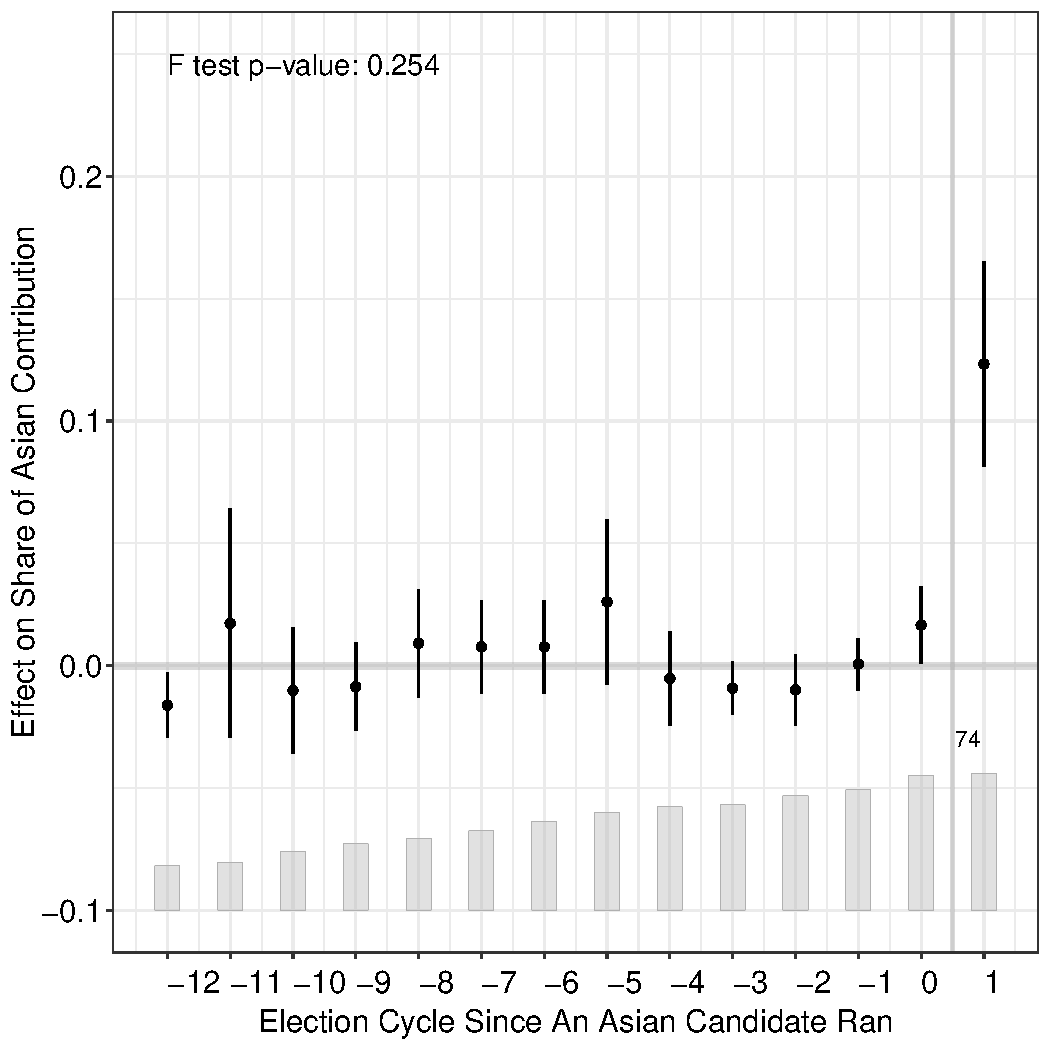
\includegraphics[width = 0.28\textwidth]{apps/gs2020_fect.pdf}}\hspace{1em}
  \subfigure[Placebo test]{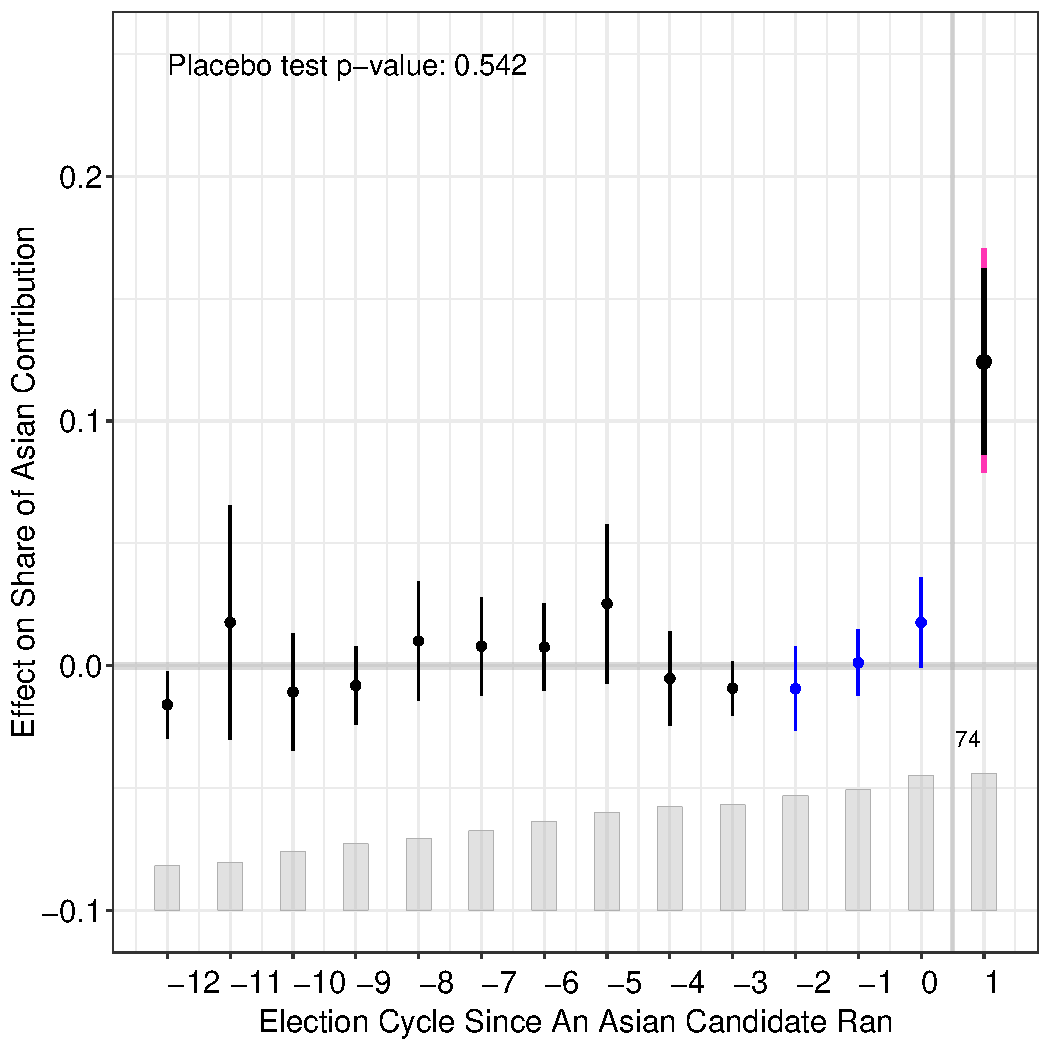
\includegraphics[width = 0.28\textwidth]{figure/apps/gs2020_placebo_honest.pdf}}\hspace{1em}
  \subfigure[Test for carryover effects]{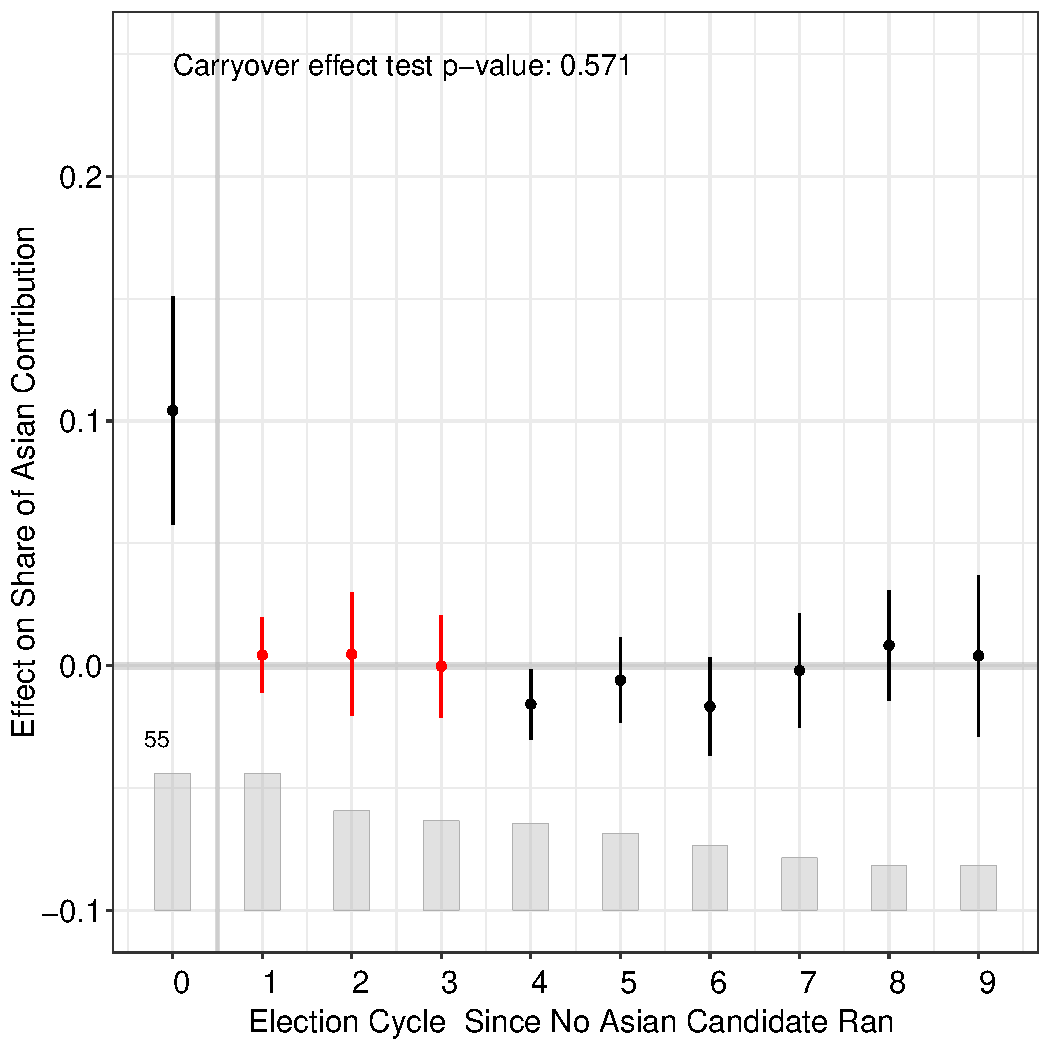
\includegraphics[width = 0.28\textwidth]{apps/gs2020_carryover.pdf}}
  \end{center}
{\footnotesize\textbf{Note:} Reanalysis of data from \citet{Grumbach2020}. Subfigures (a): Treatment effect or ATT estimates from multiple methods; subfigures (b)-(d): event-study plots using TWFE, \texttt{PanelMatch}, and \texttt{FEct}; Subfigure (e)-(f): results from the placebo test and test for carryover effects using \texttt{FEct}---the blue points in (g) and red points in (h) represent the holdout periods in the respective tests. CIs for TWFE, \texttt{PanelMatch}, and \texttt{FEct} In all subfigures are produced by bootstrap percentile methods. The robust confident set for the ATT ($\bar{M} = 0.5$) is shown in pink in (e).}} \end{minipage}\vspace{-0.5em}
  \end{figure}

Next, we conduct diagnostic tests based on \texttt{FEct} to further assess how plausible the PTA is  (including the $F$ test and the placebo test) and, in applications with treatment reversal, the no-carryover-effect assumption. We use \texttt{FEct} because it is applicable across all studies in our replication sample and does not discard data. Figures~\ref{fg:gs2020}(d), (e) and (f) show the results from the $F$ test, placebo test, and test for no carryover effects on our running example, respectively. Both a visual inspection and the formal tests suggest that the PTA and the no-carryover-effect assumption are quite plausible. 

One important caveat is that the results of these tests may either suffer from low power with a small sample size or be ``too powerful'' with abundant data.\footnote{By a test being too powerful, we mean that it has power against alternatives that are very close to the null (which might occur, for example, in the presence of an outlier or a marginally consequential confounder) and unlikely to be a source of significant bias in the treatment effect estimates.} To address the latter concern, we also perform an equivalence test of the null that pretreatment effects are ``large,'' i.e. outside some $\theta$-neighborhood of 0. Note this test requires us to specify a threshold $\theta$, and we conduct tests with a default threshold and with the ATT set as the threshold.\footnote{We provide the implementation details of all tests mentioned in this section in Section A.4. of the SM and refer readers to \citet{LWX2022} for more details on all the tests we use, including how $\theta$ is chosen.} Small $p$-values are evidence in favor of the claim that PTA violations are at most mild. 

Finally, we compute robust CSs proposed by \citet{rambachan2023more} that allow for PTA violations under relative magnitude (RM) restrictions, which allow for post-treatment violations of the PTA that are at most $\bar{M}$ times the size of the maximum violation in pretreatment \emph{placebo} periods.\footnote{We use pretreatment placebo periods as the benchmark because placebo estimates are estimated in the same way as post-treatment ATT estimates \citep{Roth2024interpret}.} In other words, the differential trend between any two consecutive post-treatment periods are assumed to be no greater than $\bar{M}$ times the maximum difference between any two placebo periods. If we first assume we can decompose each estimator for the DTE $\beta_t$ into the actual DTE $\tau_t$ and a trend component $\delta_t$, $\beta_t=\tau_t+\delta_t$, then the RM assumption requires that for all periods relative to treatment $t$, 
\begin{center}
    $|\delta_{t+1}-\delta_t| \leq \bar{M} \cdot \max_{s\in \mathcal{P}\backslash\{0\}}\{\delta_{s+1} - \delta_s\}$. 
\end{center}
in which $\mathcal{P}$ is the set of placebo periods. In our case, we use $\mathcal{P}=\{-2, -1, 0\}$, meaning the maximum trend is given by $\max\{\delta_{0}-\delta_{-1}, \delta_{-1}-\delta_{-2}\}$. Robust CSs are uniformly valid for the partially identified treatment effects under the RM restriction. \citet[][p. 2653]{rambachan2023more} suggest $\bar{M}=1$ as a ``natural benchmark'' with similar numbers of pretreatment and post-treatment periods, corresponding to the assumption that any PTA violations are no worse than the observed pretrend.
For each paper, we compute the robust CSs with $\bar{M}=0.5$, erring on the lenient side. We also conduct a sensitivity analysis for each such study, obtaining the ``breakdown value'' of $\bar{M}$, denoted as $\tilde{M}$, at which the robust CS first includes zero. Figure~\ref{fg:gs2020}(e) marks the robust CS for the ATT estimated by \texttt{FEct} in pink. In this example, the robust CS excludes zero, and the breakdown value from the sensitivity analysis is $\tilde{M}=3.0$, suggesting that the estimated coethnic mobilization effect is robust to potential violations of the PTA under the RM restriction. 

Overall, the results from \citet{Grumbach2020} appear highly robust, regardless of the choice of point and variance estimators. The study seems to have sufficient power to evaluate and instill confidence in the validity of its identification assumptions and to distinguish the ATT from zero, even under violations of the PTA. There are also little to no carryover effects.

%  
\FloatBarrier

%  $$$$$$\                                                                      
% $$  __$$\                                                                     
% $$ /  \__|$$\   $$\ $$$$$$\$$$$\  $$$$$$\$$$$\   $$$$$$\   $$$$$$\  $$\   $$\ 
% \$$$$$$\  $$ |  $$ |$$  _$$  _$$\ $$  _$$  _$$\  \____$$\ $$  __$$\ $$ |  $$ |
%  \____$$\ $$ |  $$ |$$ / $$ / $$ |$$ / $$ / $$ | $$$$$$$ |$$ |  \__|$$ |  $$ |
% $$\   $$ |$$ |  $$ |$$ | $$ | $$ |$$ | $$ | $$ |$$  __$$ |$$ |      $$ |  $$ |
% \$$$$$$  |\$$$$$$  |$$ | $$ | $$ |$$ | $$ | $$ |\$$$$$$$ |$$ |      \$$$$$$$ |
%  \______/  \______/ \__| \__| \__|\__| \__| \__| \_______|\__|       \____$$ |
%                                                                     $$\   $$ |
%                                                                     \$$$$$$  |
%                                                                      \______/ 
                                                                           

                                                                              
\section{Systematic Assessment}\label{sc:results}

We perform the replication and reanalysis procedure described above for all 37 articles in our sample. This section offers a summary of our findings; complete results for each paper are available in the SM. We organize our results around two main questions: (1) Do HTE-robust estimators yield qualitatively different results compared to those obtained with TWFE? (2) Is the PTA plausible, and do original findings (where null hypotheses are rejected) remain robust against HTE and potential PTA violations? Additionally, we discuss other issues observed in the replicated articles, including the presence of carryover effects and sensitivity to model specifications.




% $$\   $$\ $$$$$$$$\ $$$$$$$$\ 
% $$ |  $$ |\__$$  __|$$  _____|
% $$ |  $$ |   $$ |   $$ |      
% $$$$$$$$ |   $$ |   $$$$$\    
% $$  __$$ |   $$ |   $$  __|   
% $$ |  $$ |   $$ |   $$ |      
% $$ |  $$ |   $$ |   $$$$$$$$\ 
% \__|  \__|   \__|   \________|
                             
%\FloatBarrier

\paragraph*{HTE-robust estimators yield qualitatively similar but highly variable findings.}

To examine the possible impact of the weighting problem caused by HTE, we first compare the estimates obtained from the imputation estimator, \texttt{FEct}, for all studies to those originally reported. The dissimilarity between the original and \texttt{FEct} estimates proxies the extent to which the negative weighting problem is consequential in practice. Figure~\ref{fg:twfe-v-hte}(a) plots the comparison. The horizontal axis represents the originally reported TWFE estimates, and the vertical axis represents estimates from \texttt{FEct}, both normalized using the same originally reported SE. If the point estimates are identical, then the corresponding point should lie exactly on the 45-degree line (dashed). Red solid circles represent studies whose \texttt{FEct} estimates are not significant at the 5\% level based on cluster-bootstrapped CIs. Observe that the points largely follow the 45-degree line, and that \texttt{FEct} \emph{always} has the same sign as the original estimate. This suggests that scenarios where accounting for HTE entirely reverses the empirical findings, while theoretically possible, are rare. 

This said, results do sometimes deviate significantly. In the extremes, we observe \texttt{FEct} estimates as small as a fourth of or as large as over twice the TWFE estimate. In the SM, we include a plot of the ratios of the estimates. The most consequential deviations correspond to studies that were originally on the margins of statistical significance. 
Alarmingly, when switching from TWFE to \texttt{FEct}, the number of studies that are statistically insignificant at the 5\% level rises from one to 11.\footnote{This is due to a combination of drops in point estimates and larger SEs. See Section A.5. in the SM for more details.} This group constitutes 28\% of all articles and disproportionately consists of studies whose original $z$ scores are smaller than three. We further discuss the consequences on power and inference later. 


\begin{figure}[!ht]
  \caption{Comparison of Estimates: TWFE vs. HTE-Robust Estimators}\label{fg:twfe-v-hte}
  \centering
  \vspace{-0.5em}
  \begin{minipage}{1\linewidth}{
  \begin{center}  
  \subfigure[Comparison of \texttt{FEct} and TWFE estimates]{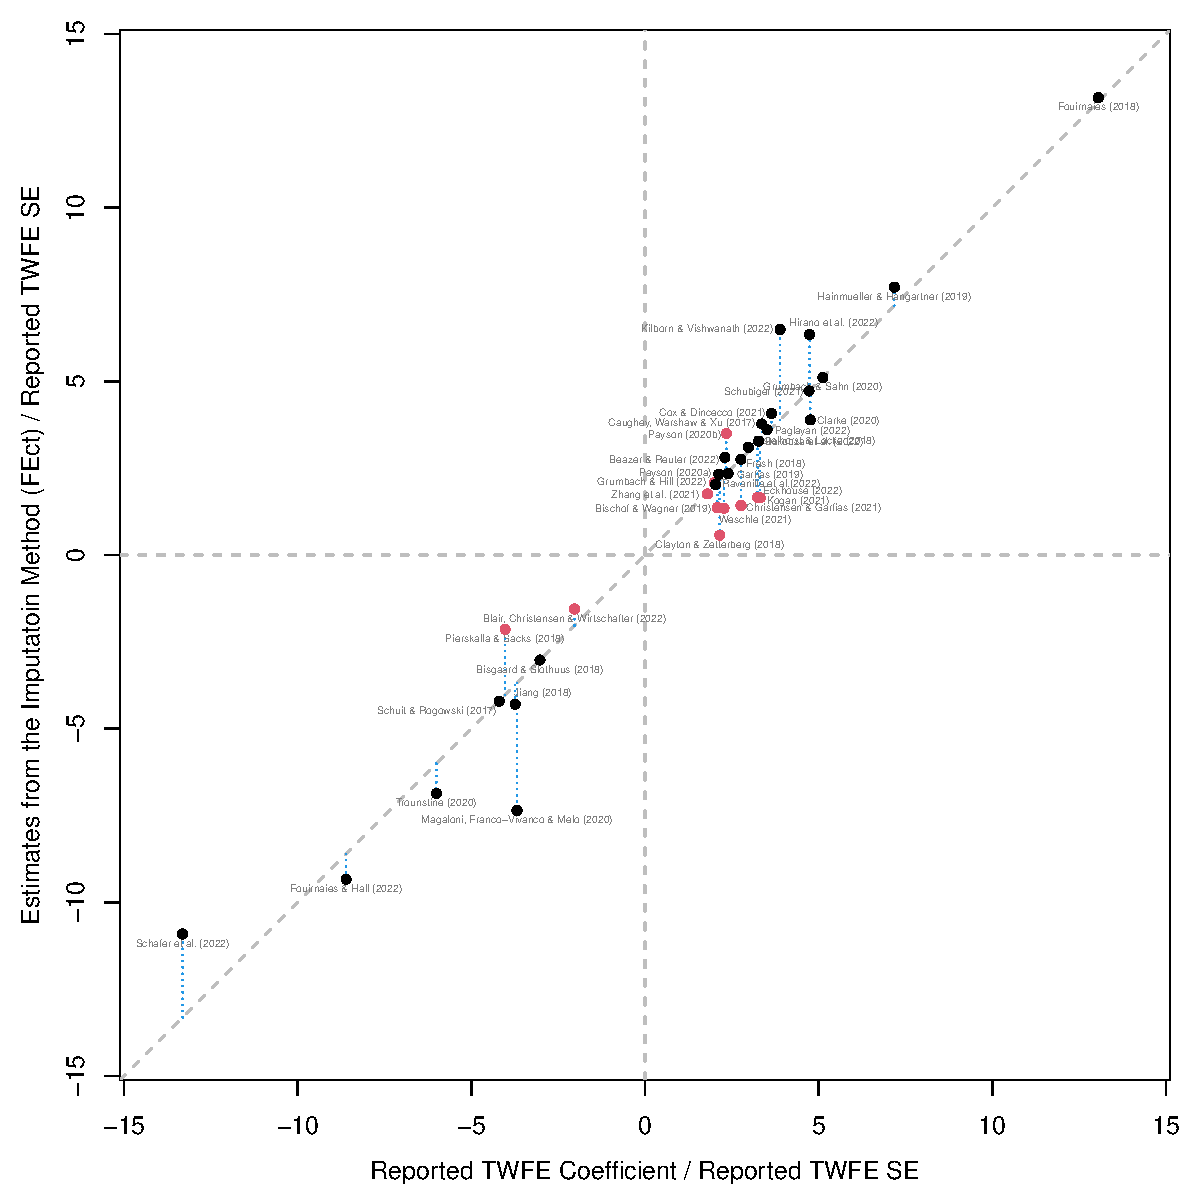
\includegraphics[width = 0.45\textwidth]{summary/est_all.pdf}}
  \vspace{-1em}
  \hspace{1em}
  \subfigure[Comparison of HTE-robust and TWFE estimates in the staggered setting]{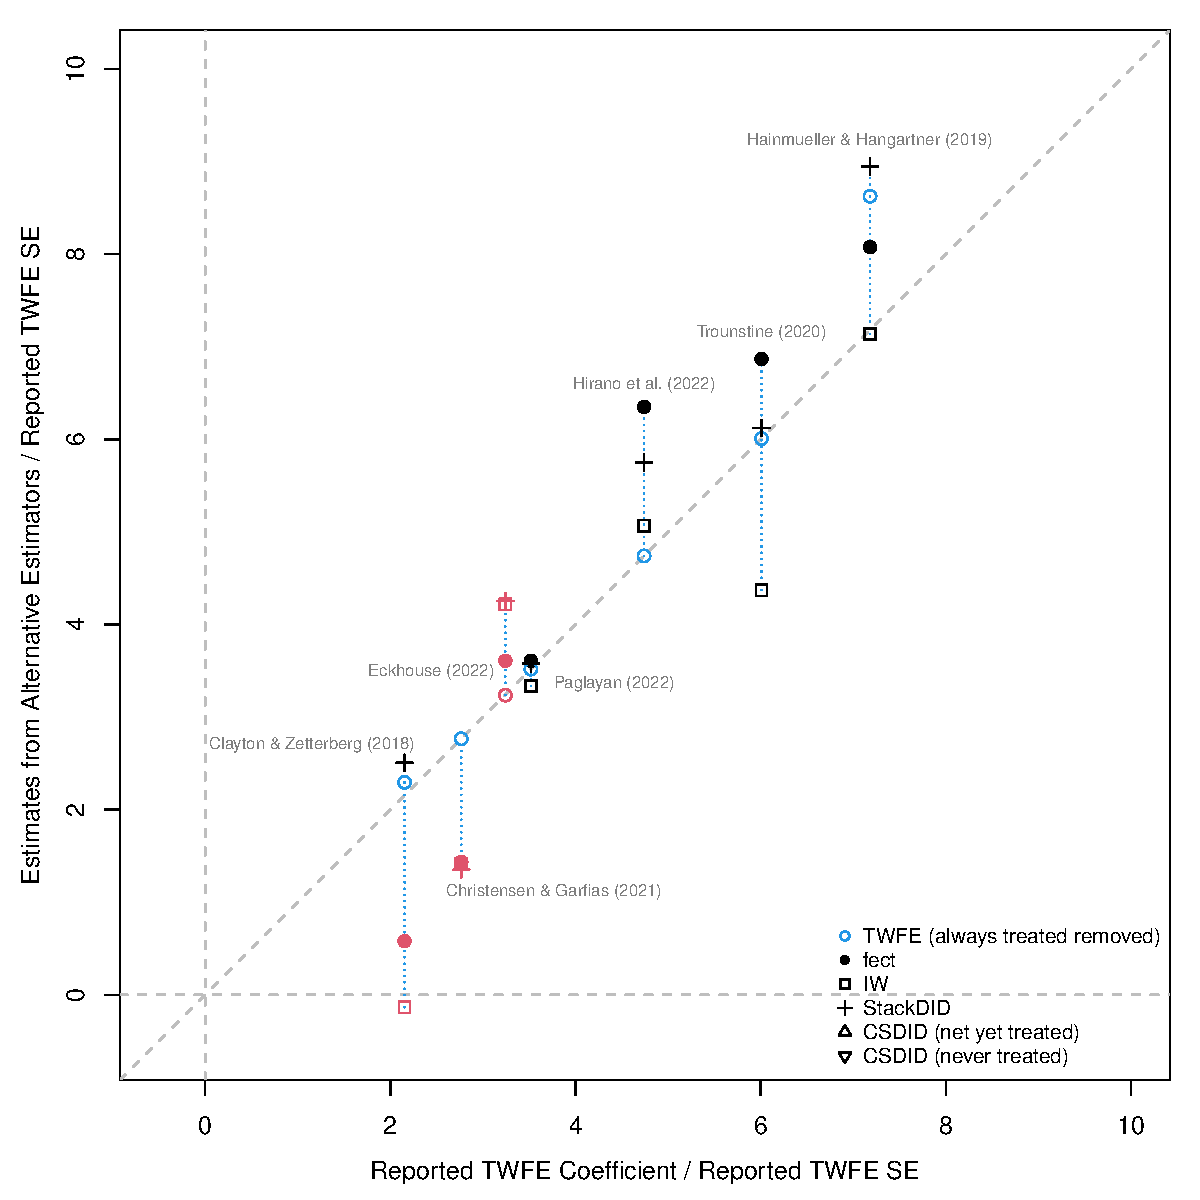
\includegraphics[width = 0.45\textwidth]{summary/est_staggered.pdf}}
  \end{center}
  {\footnotesize\textbf{Note:} Subfigure (a) compares TWFE coefficients and estimates from the imputation method (\texttt{FEct}). Estimates for each application are normalized by the same TWFE SE. \cite{fh2018} and \citet{Hall2022} are close to the 45-degree line but not included in the figure as their TWFE $z$-scores are above 15. Subfigure (b) compares reported coefficients and estimates from various alternative estimators. All seven estimates for each application are normalized by the same reported SE. We multiply the estimates by $Sign(\hat\delta^{TWFE}$) for easier visualization.  In both figures, red symbols represent studies whose ATT estimates from the respective HTE-robust estimators are statistically insignificant at the 5\% level based on bootstrapped CIs. 
  }}
  \end{minipage}\vspace{-1em}
\end{figure}
%in other words, we flip the signs of all estimates for applications with a negative TWFE estimate.

If we restrict our attention to the staggered case, we can broaden our comparison set to include all HTE-robust estimators discussed earlier.\footnote{\citet{Kogan2021} and \citet{magaloni2020killing} are not included because the original specifications include additional time trends, which are not supported by HTE-robust estimators except \texttt{FEct}.} Figure~\ref{fg:twfe-v-hte}(b) plots the point estimates for these cases obtained from each HTE-robust estimator, in addition to TWFE, all normalized by the reported SE. The estimates from all HTE-robust estimators are qualitatively similar to each other, though there is a noticeable amount of variation and one sign change. As before, this spread does not change substantive findings for studies with highly substantively significant results. Furthermore, our more extensive analyses of each individual paper in the SM show that the DTE estimates from various HTE-robust estimators also generally align with each other and with those from the dynamic specification of the TWFE model. 

It is worth noting that while only a small fraction of studies in our sample (five articles, 13.5\%) employ a bootstrap procedure to estimate SEs or CIs, the widely practiced cluster-robust SE typically performs adequately because the number of clusters/units is usually fairly large. There are two examples that were significant at the $5\%$ level using cluster-robust SEs but fell below this threshold when using cluster-bootstrapped SEs, both of which were already on the margins of significance. We provide graphs comparing reported, cluster-robust, and cluster-bootstrapped SEs in the SM. 
\FloatBarrier



% $$$$$$$\ $$$$$$$$\  $$$$$$\  
% $$  __$$\\__$$  __|$$  __$$\ 
% $$ |  $$ |  $$ |   $$ /  $$ |
% $$$$$$$  |  $$ |   $$$$$$$$ |
% $$  ____/   $$ |   $$  __$$ |
% $$ |        $$ |   $$ |  $$ |
% $$ |        $$ |   $$ |  $$ |
% \__|        \__|   \__|  \__|



\begin{figure}[!th]
\caption{Estimated Dynamic Treatment Effects}\label{fg:dynamic}
\centering\scriptsize
\begin{minipage}{1\linewidth}{
\centering
\hspace{1.5em}
\resizebox{0.9\textwidth}{!}{
\begin{tabular}{C{3.8cm}C{3.8cm}C{3.8cm}C{3.8cm}}
   \citet{Beazer2022} \newline ATT: 24.38 (8.80); \newline $p$-values: 0.22, 0.68 &  
   \citet{Bischof2019} \newline ATT:  0.08 (0.08); \newline $p$-values: 0.79, 0.26  &  
   \citet{Bisgaard2018} \newline ATT: -0.05 (0.02); \newline $p$-values: n.a., n.a.  & 
   \citet{Blair2022} \newline ATT: -0.50 (0.39); \newline $p$-values: 0.50, 0.49 \\
   \hspace{-2em} 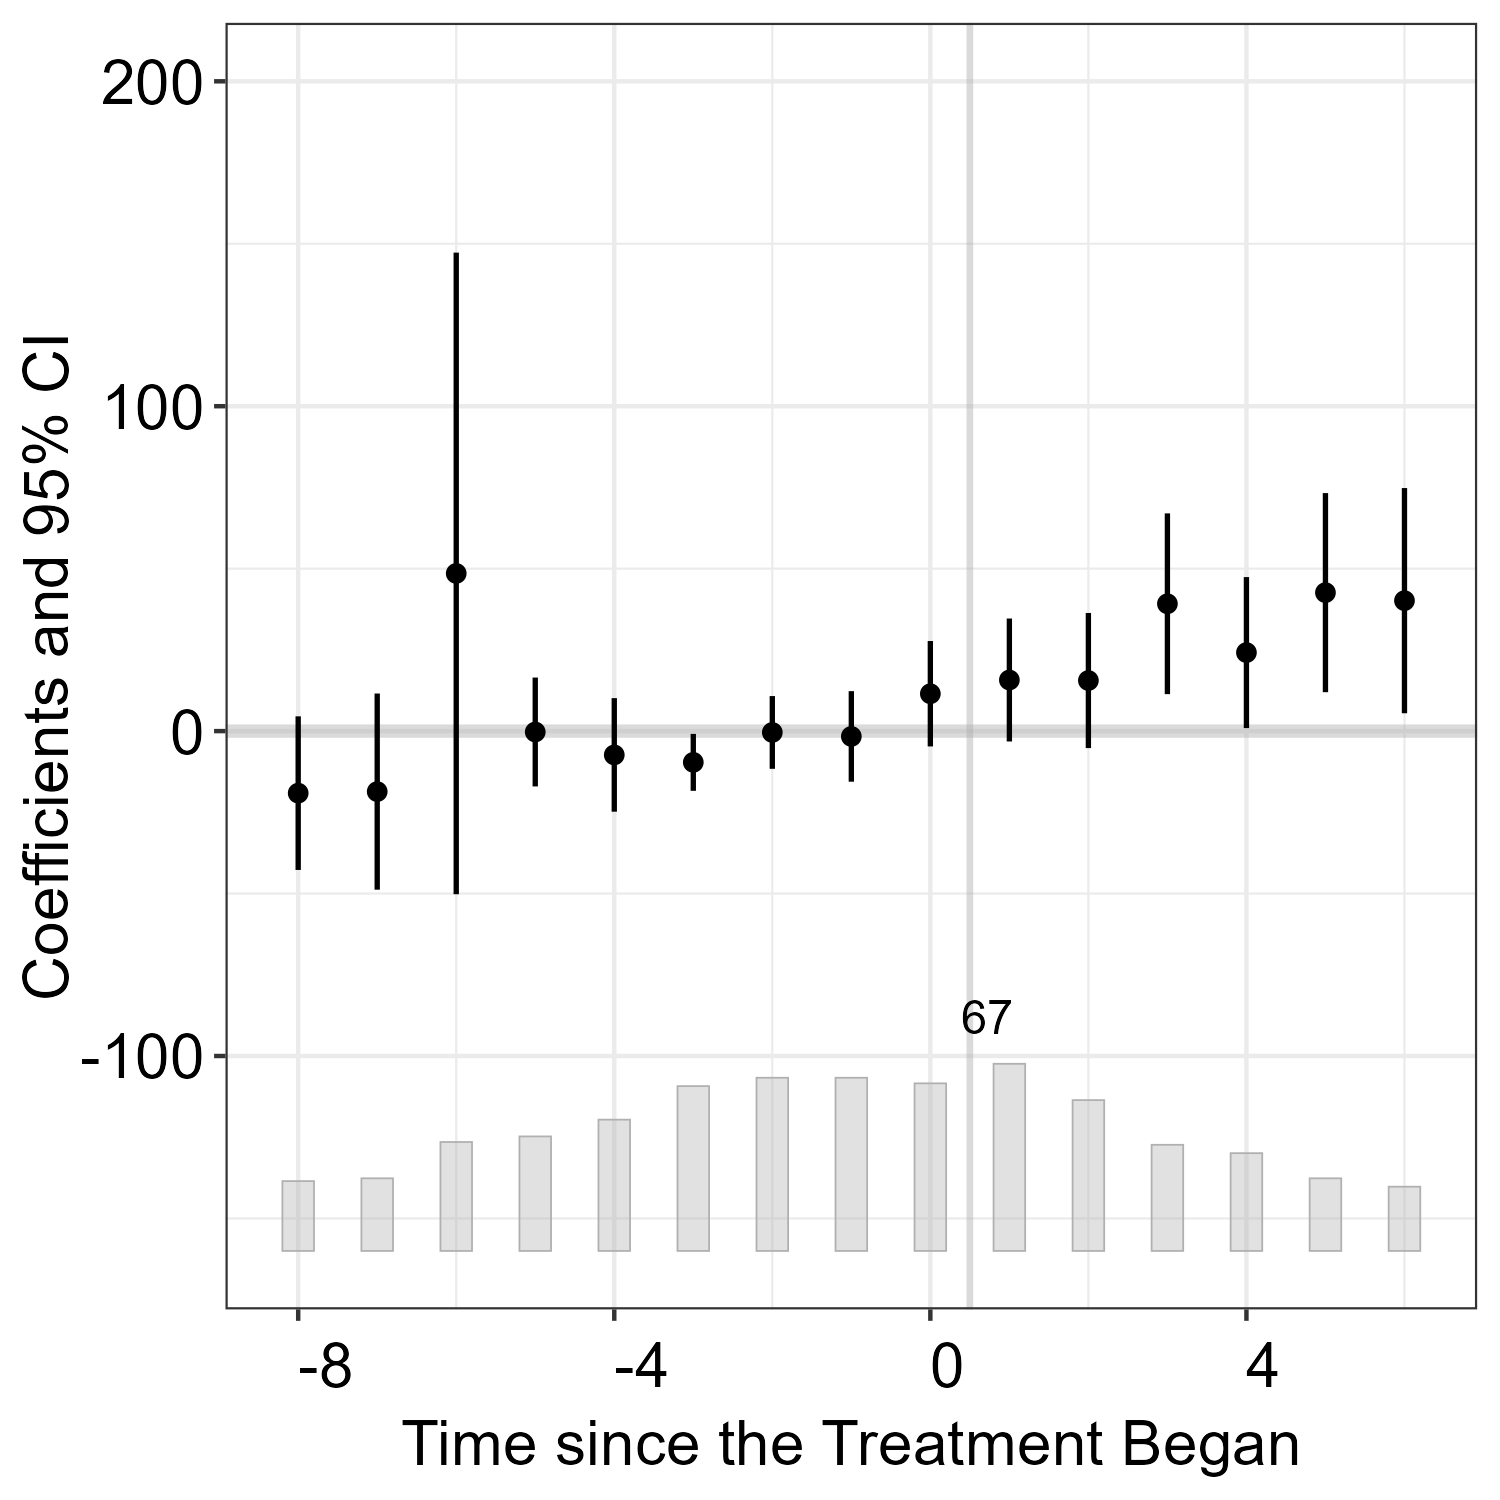
\includegraphics[width = 0.22\textwidth]{fect/beazer_fect_entry}  & 
   \hspace{-2em} 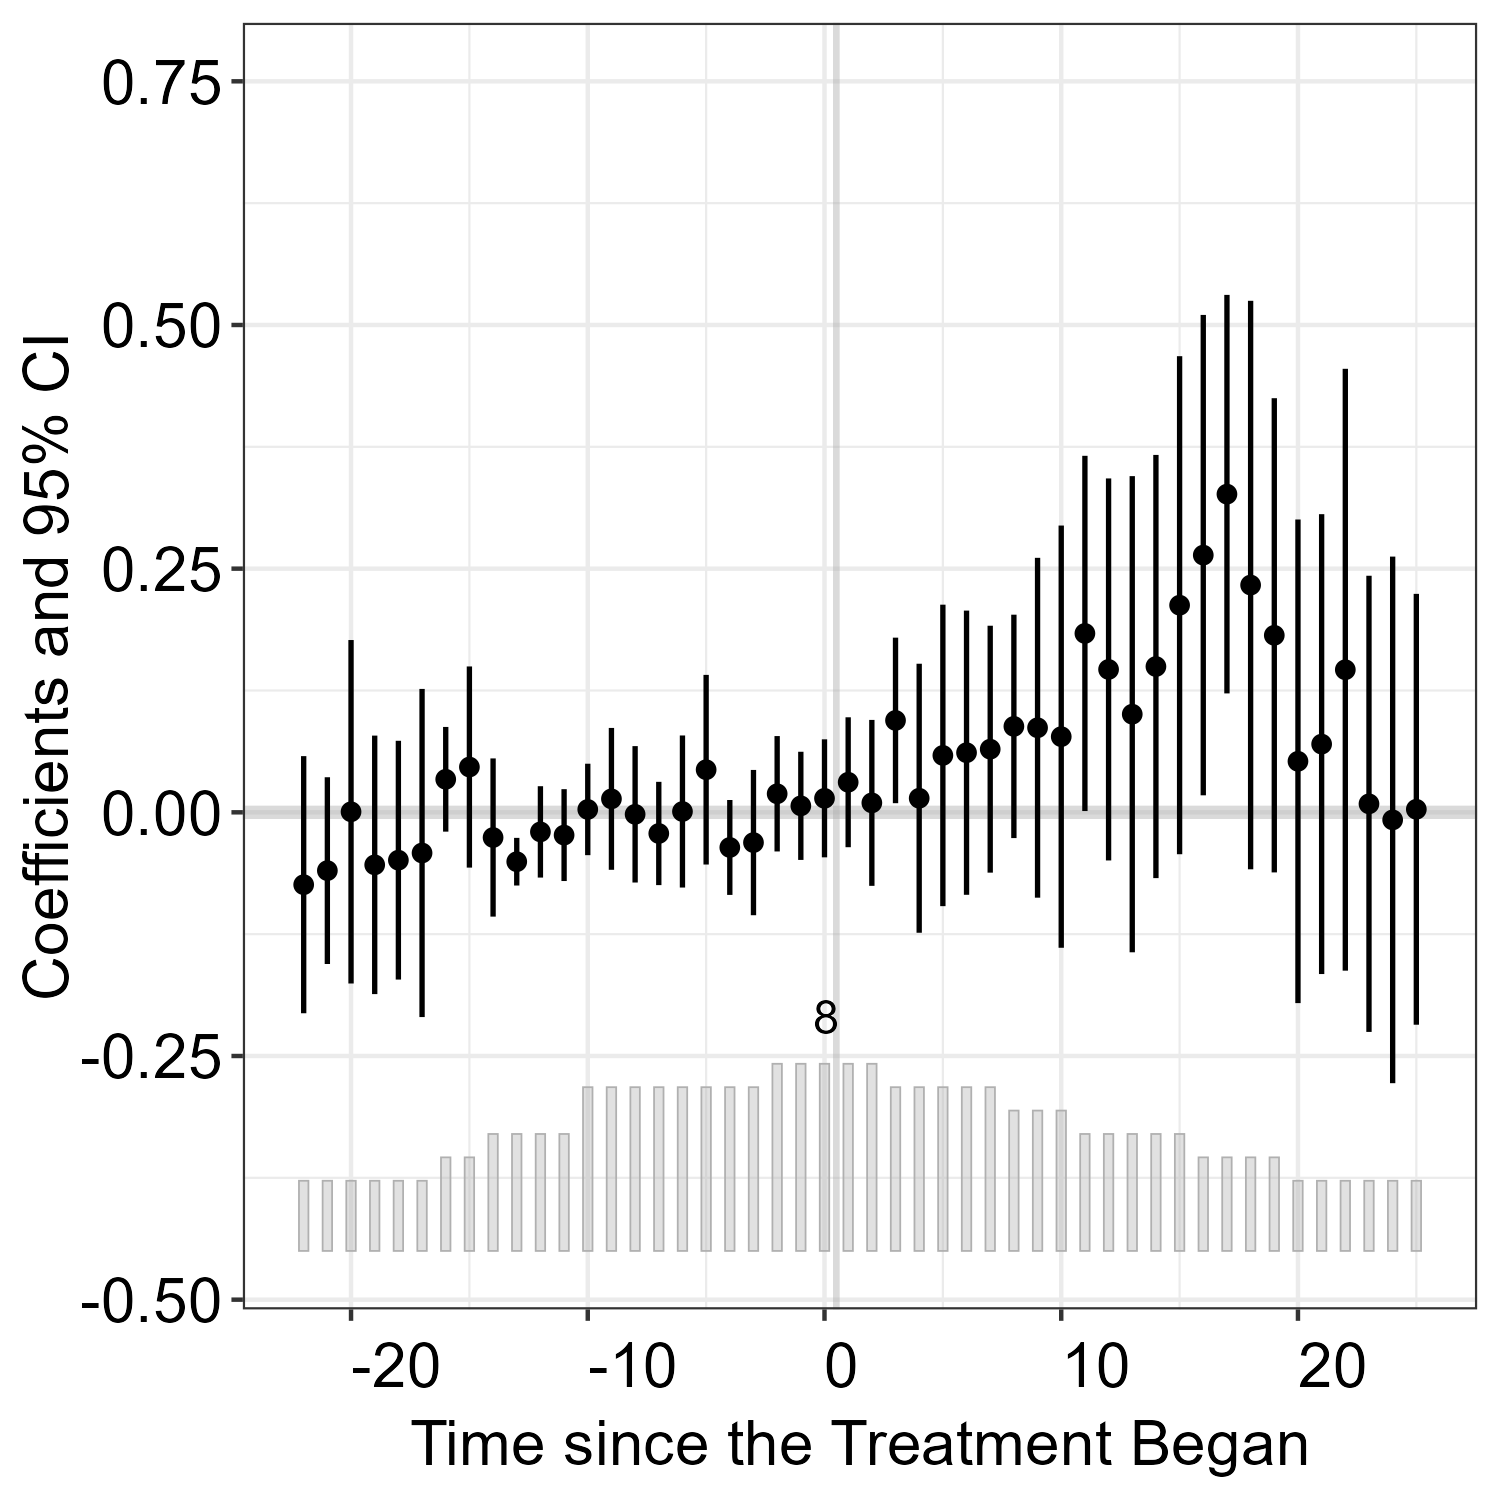
\includegraphics[width = 0.22\textwidth]{fect/bischof_fect_entry.png}  &
   \hspace{-2em} 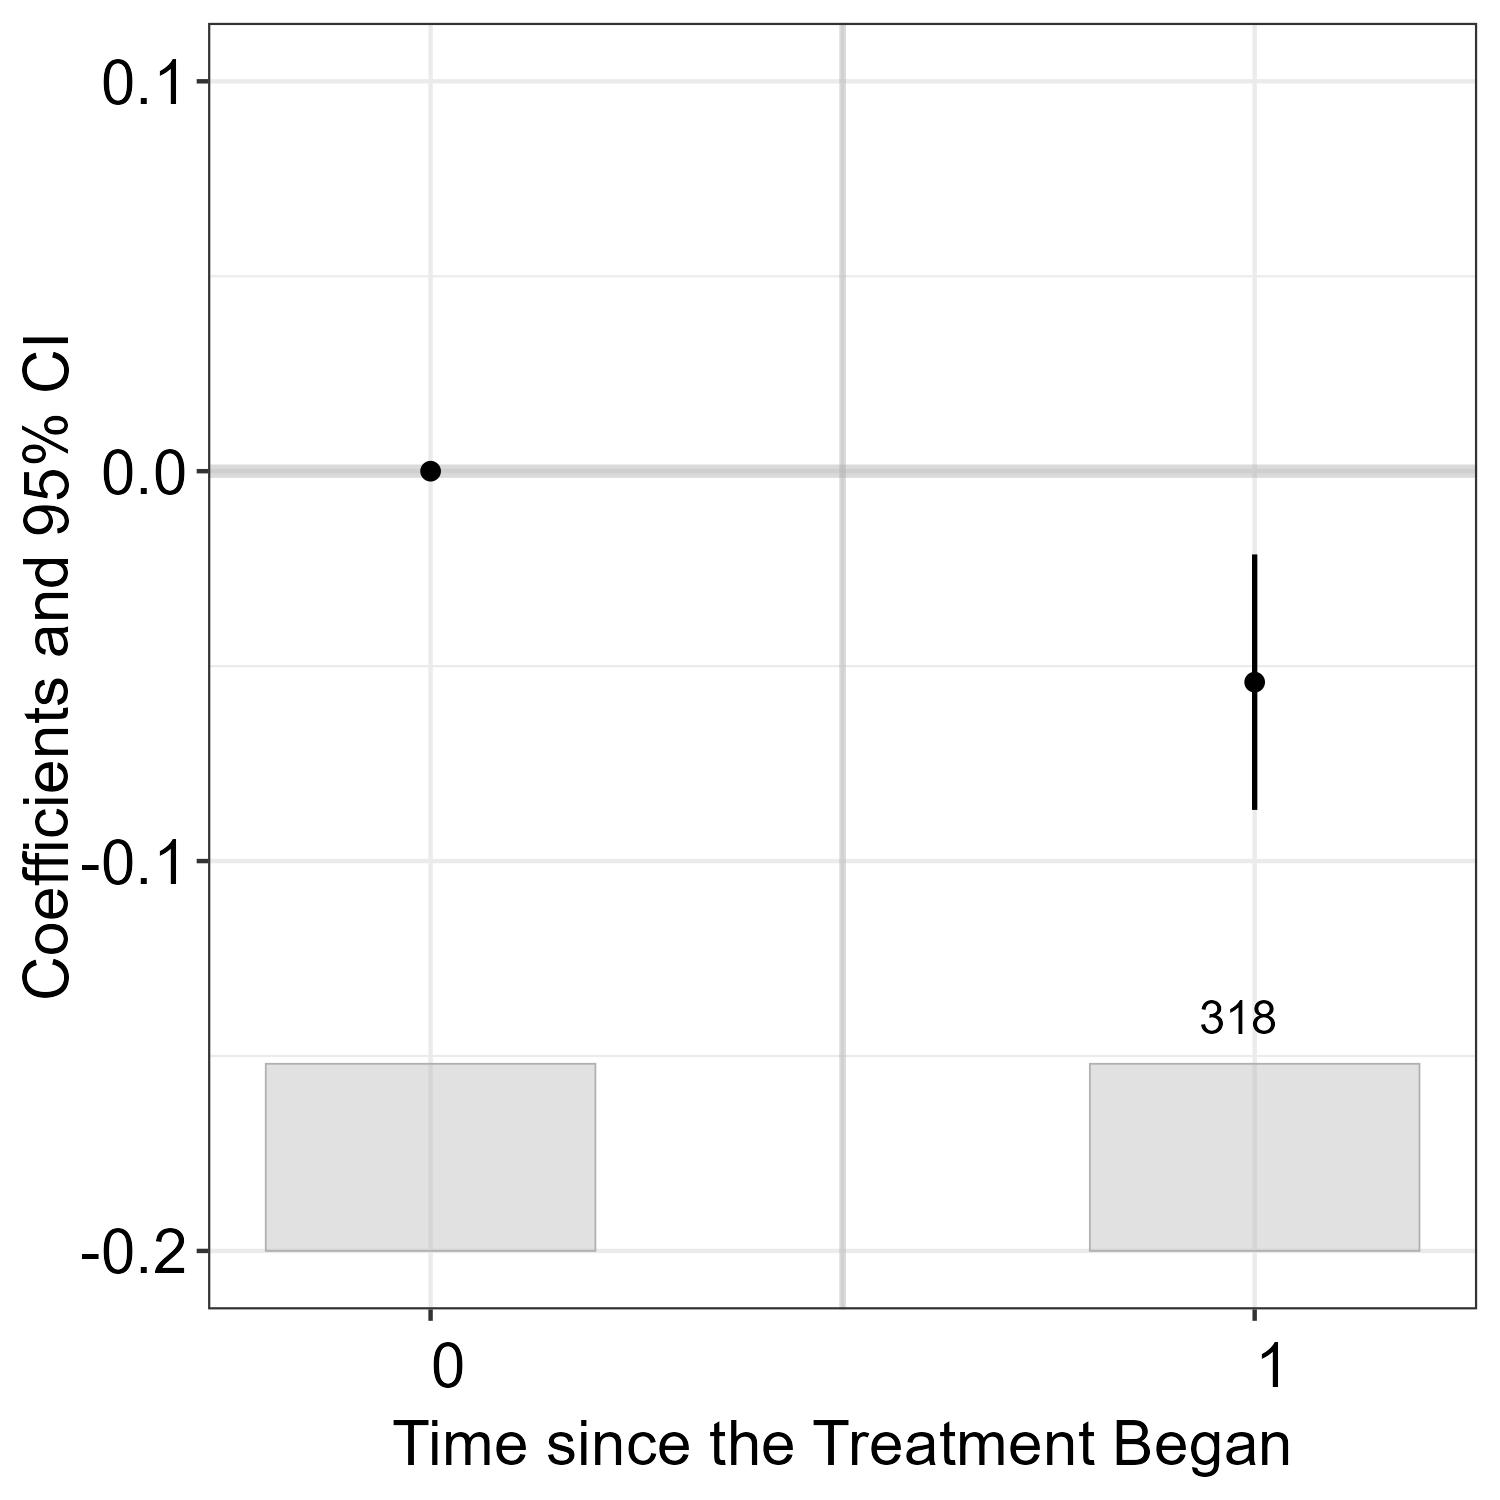
\includegraphics[width = 0.22\textwidth]{figure/fect/bisgaard_fect_entry.png}  &
   \hspace{-2em} 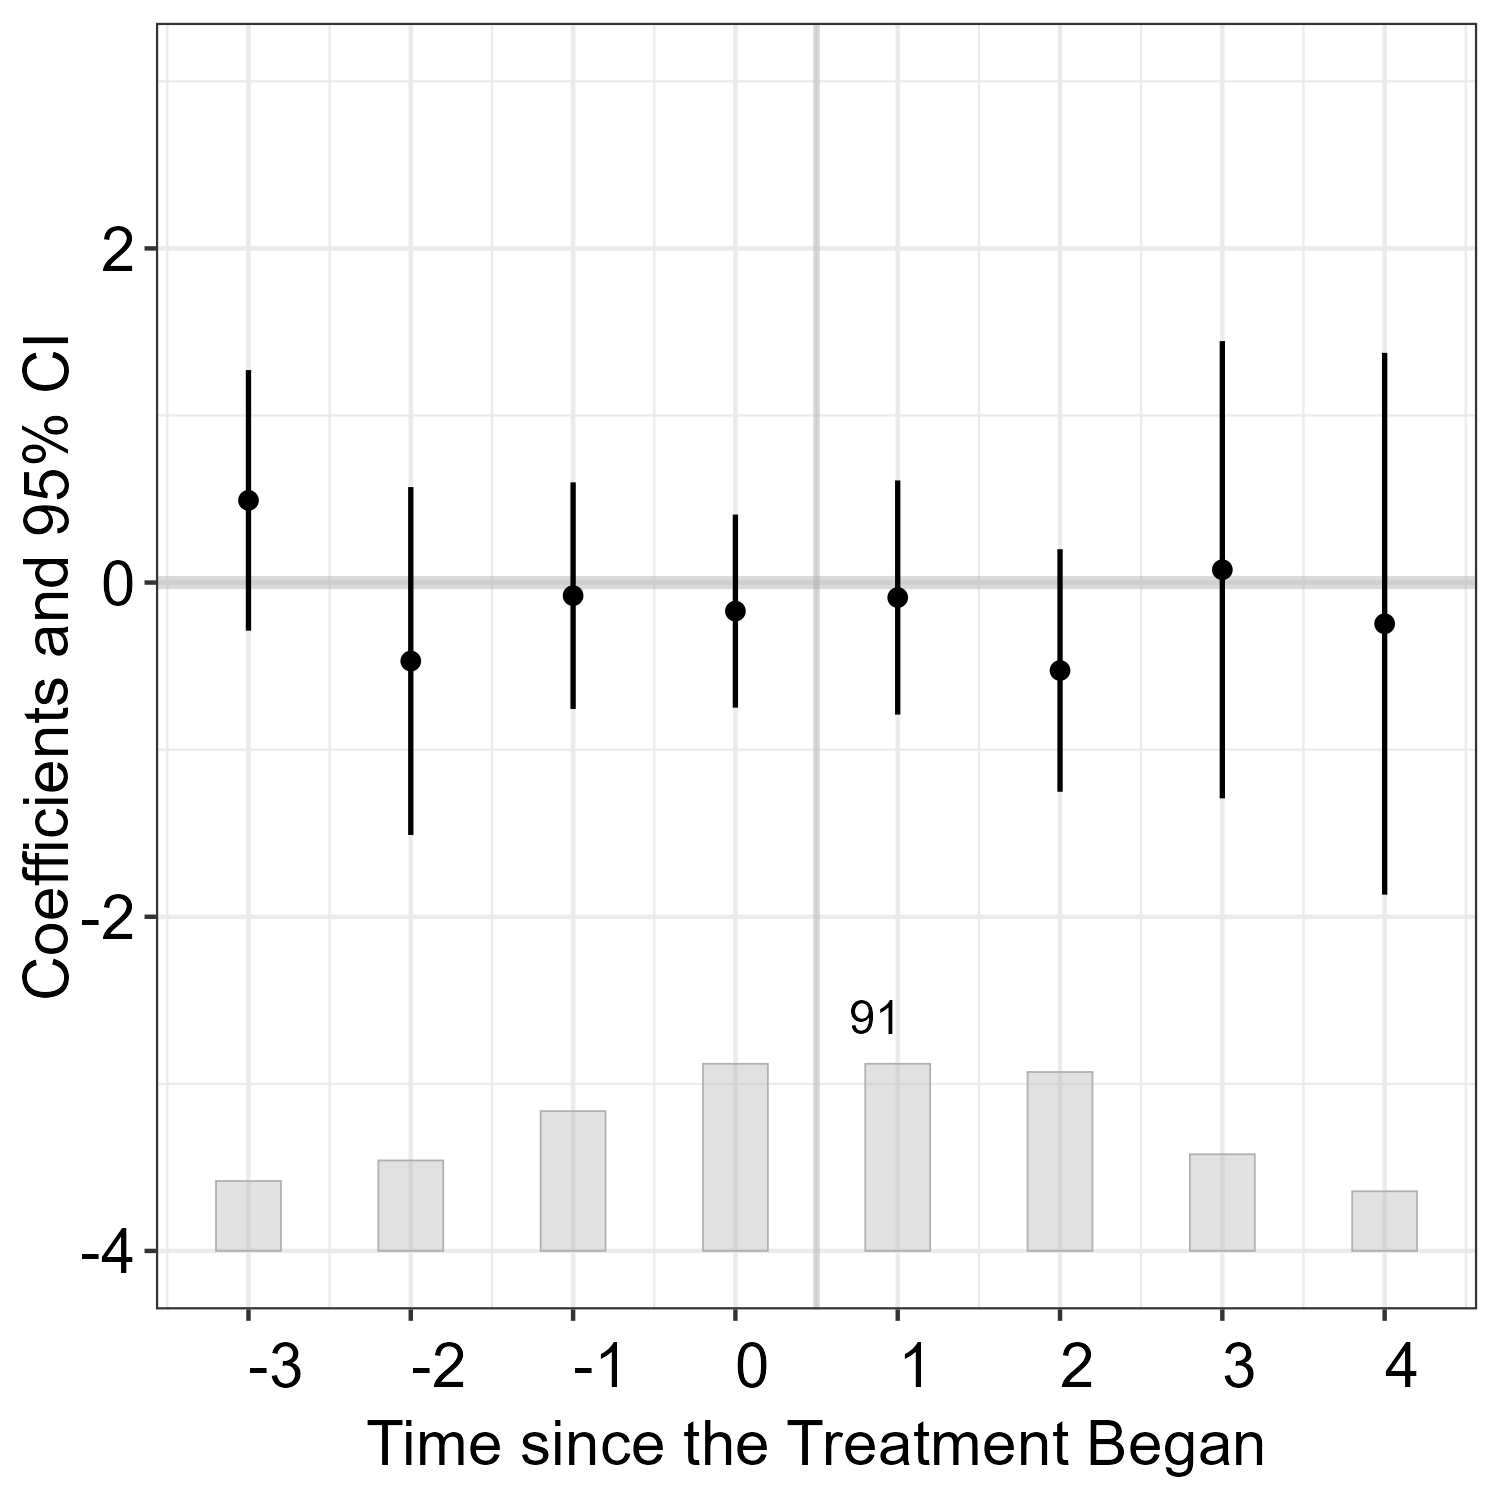
\includegraphics[width = 0.22\textwidth]{fect/blair_fect_entry}  \\ \\
   \citet{Bokobza2022} \newline ATT: 0.11 (0.03); \newline $p$-values: 0.00, 0.86 &
   \citet{Caughey2017} \newline ATT: 0.01 (0.005); \newline $p$-values: 0.04, 0.52 &  
   \citet{Christensen2021}  \newline ATT: 0.04 (0.04); \newline $p$-values: 0.72, 0.28 & 
   \citet{Clarke2020}  \newline ATT: 0.08 (0.03); \newline $p$-values: 0.38, 0.00 \\
   \hspace{-2em}  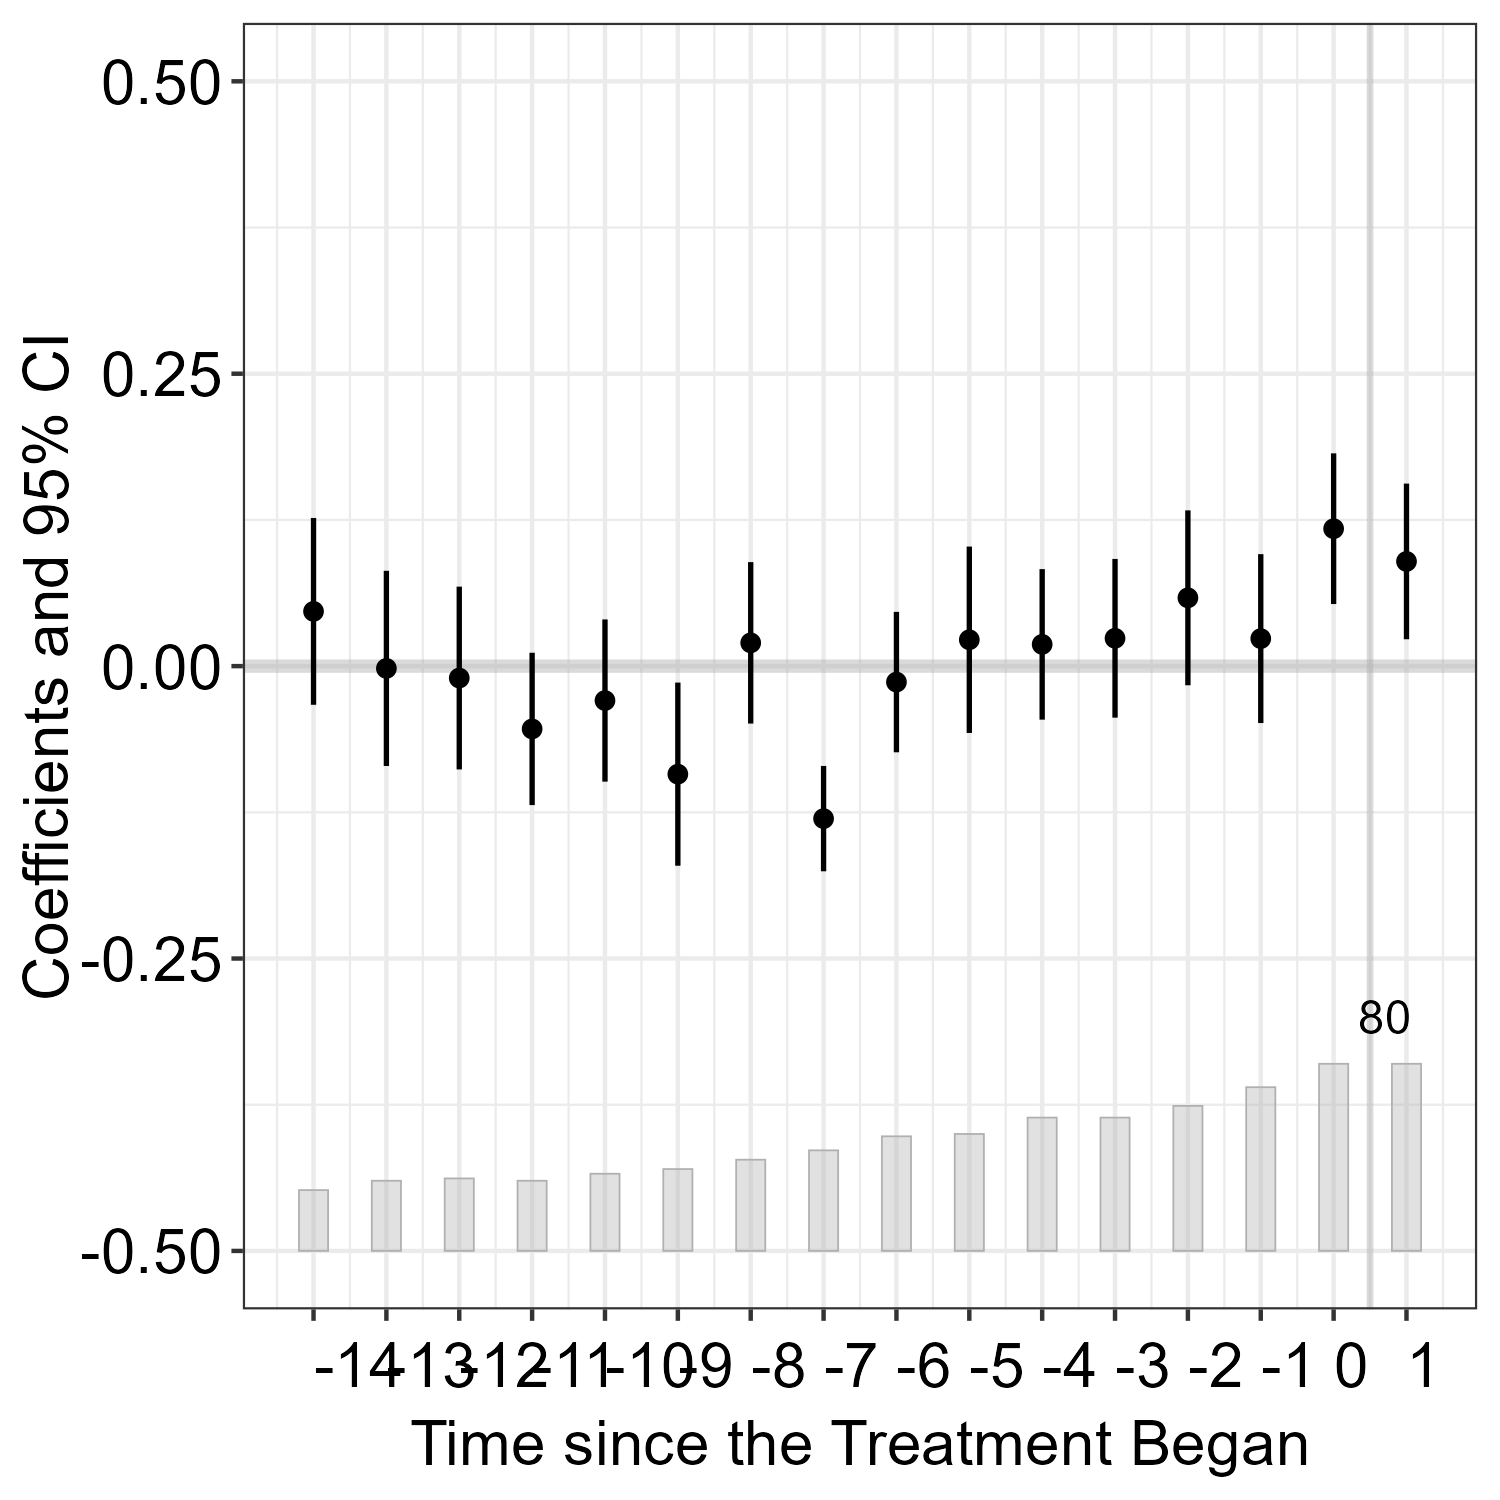
\includegraphics[width = 0.22\textwidth]{fect/bokobza_fect_entry} &
   \hspace{-2em} 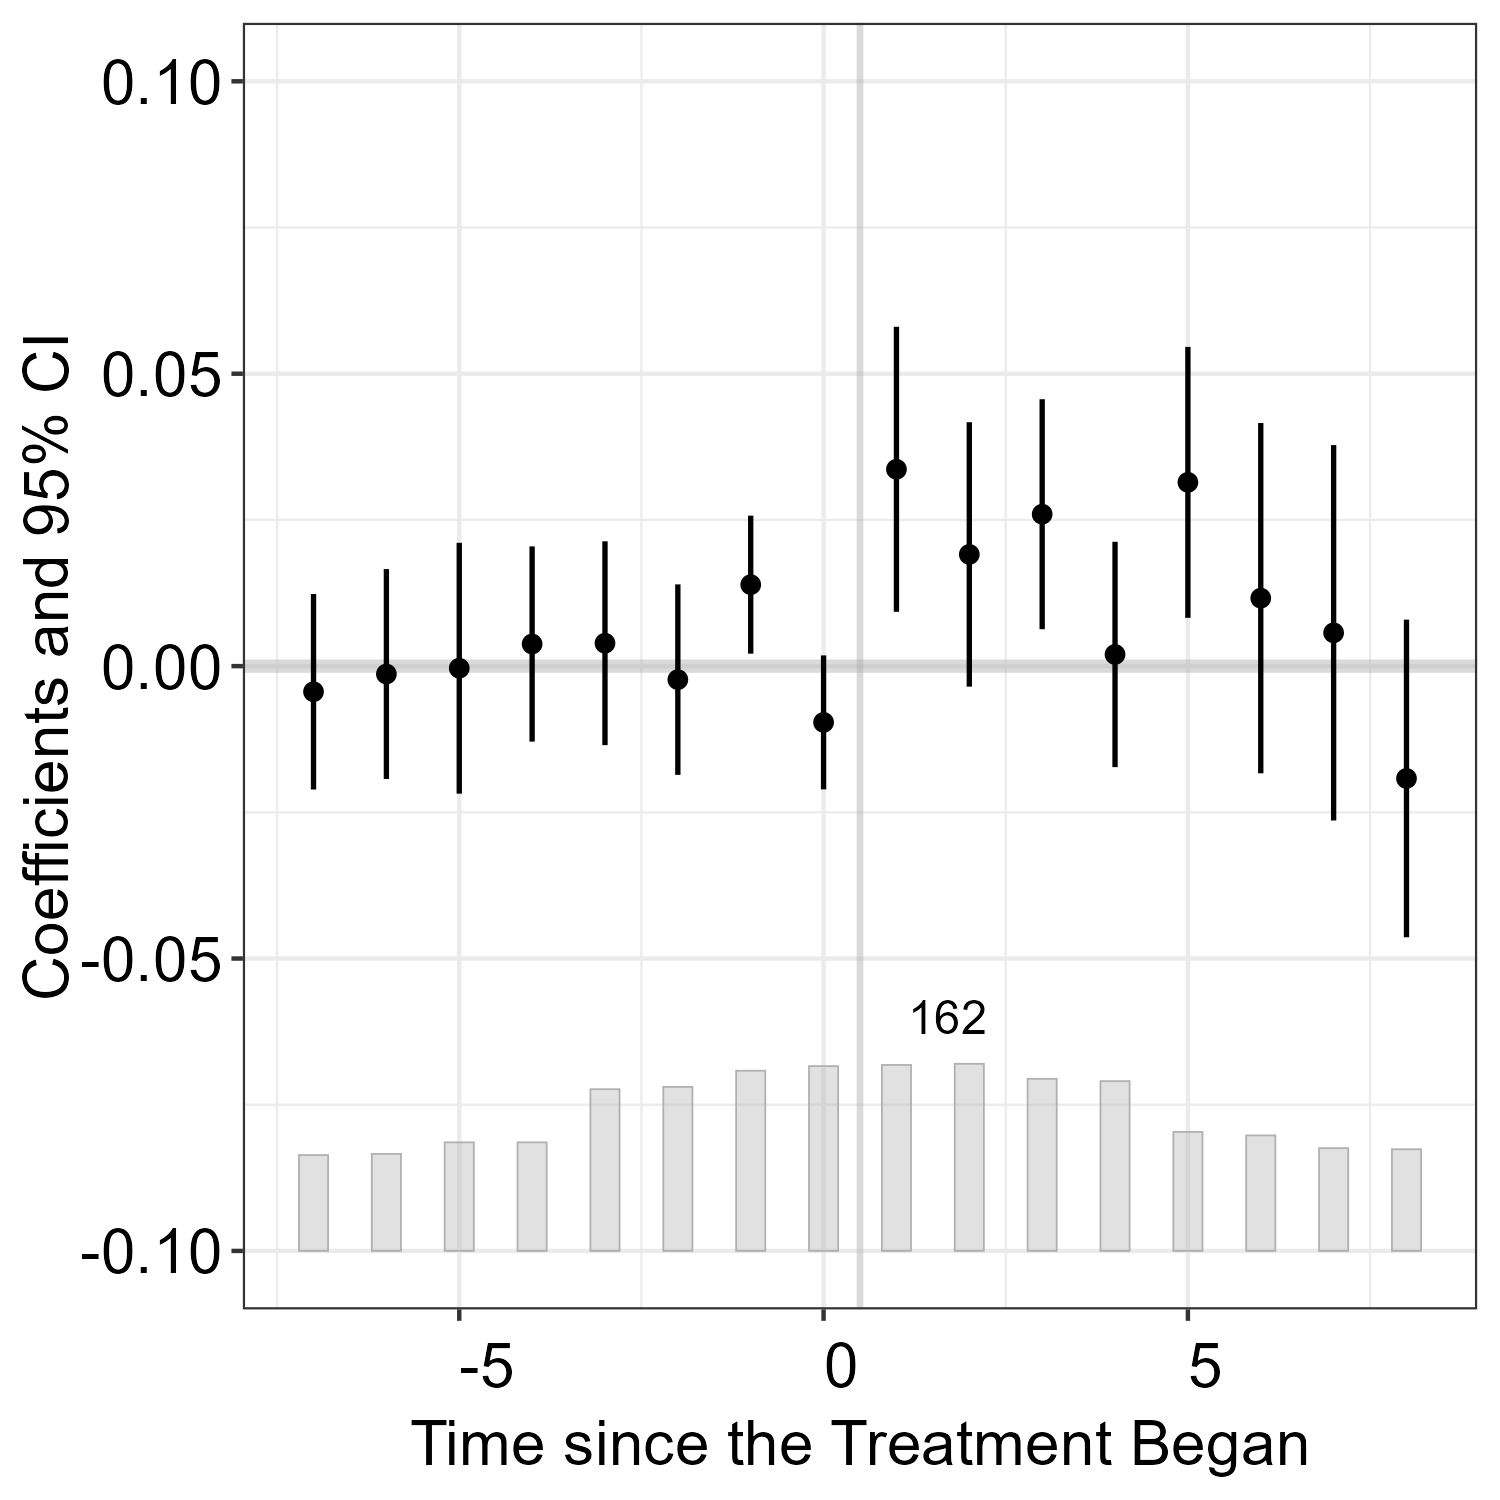
\includegraphics[width = 0.22\textwidth]{fect/Caughey_fect_entry}  &
   \hspace{-2em} 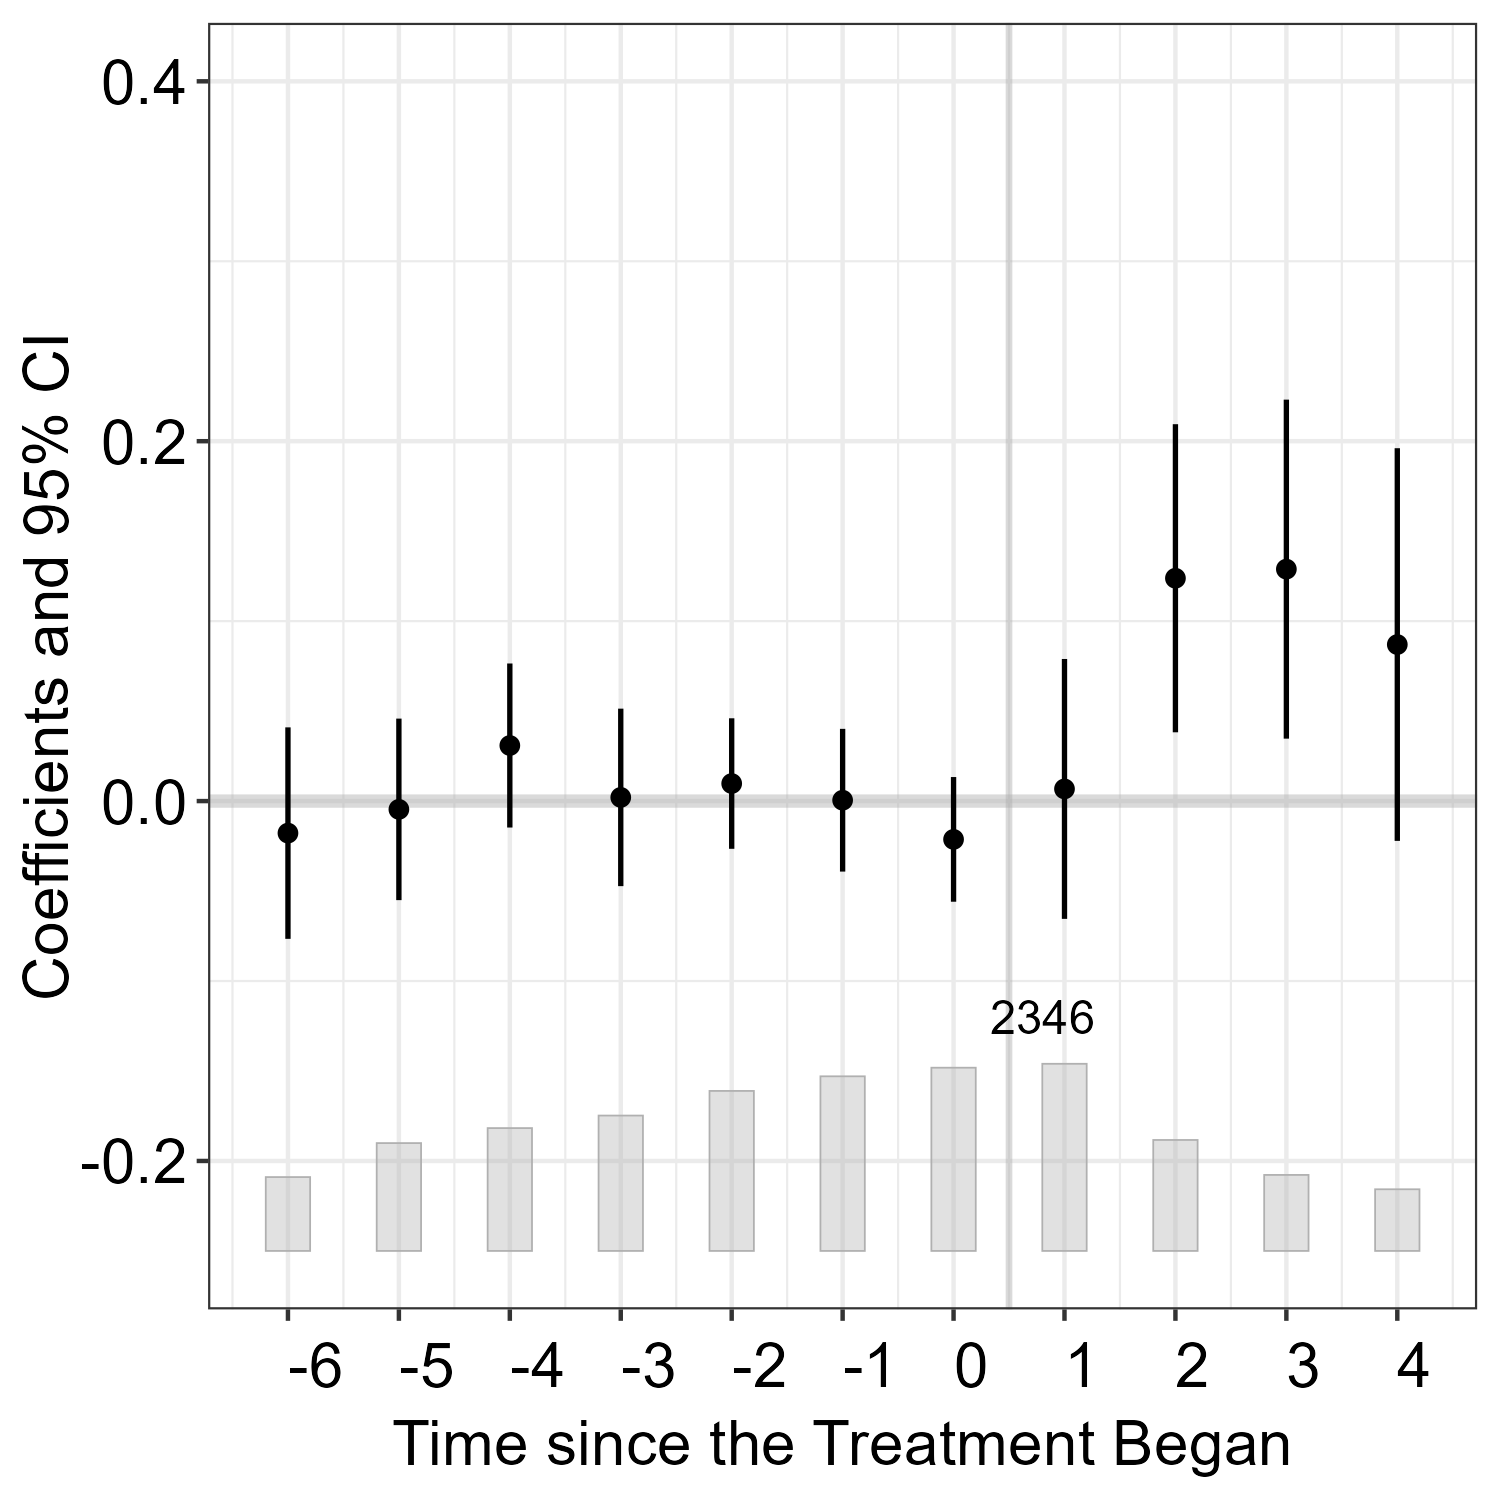
\includegraphics[width = 0.22\textwidth]{fect/chris_sub_fect_entry}  & 
   \hspace{-2em}  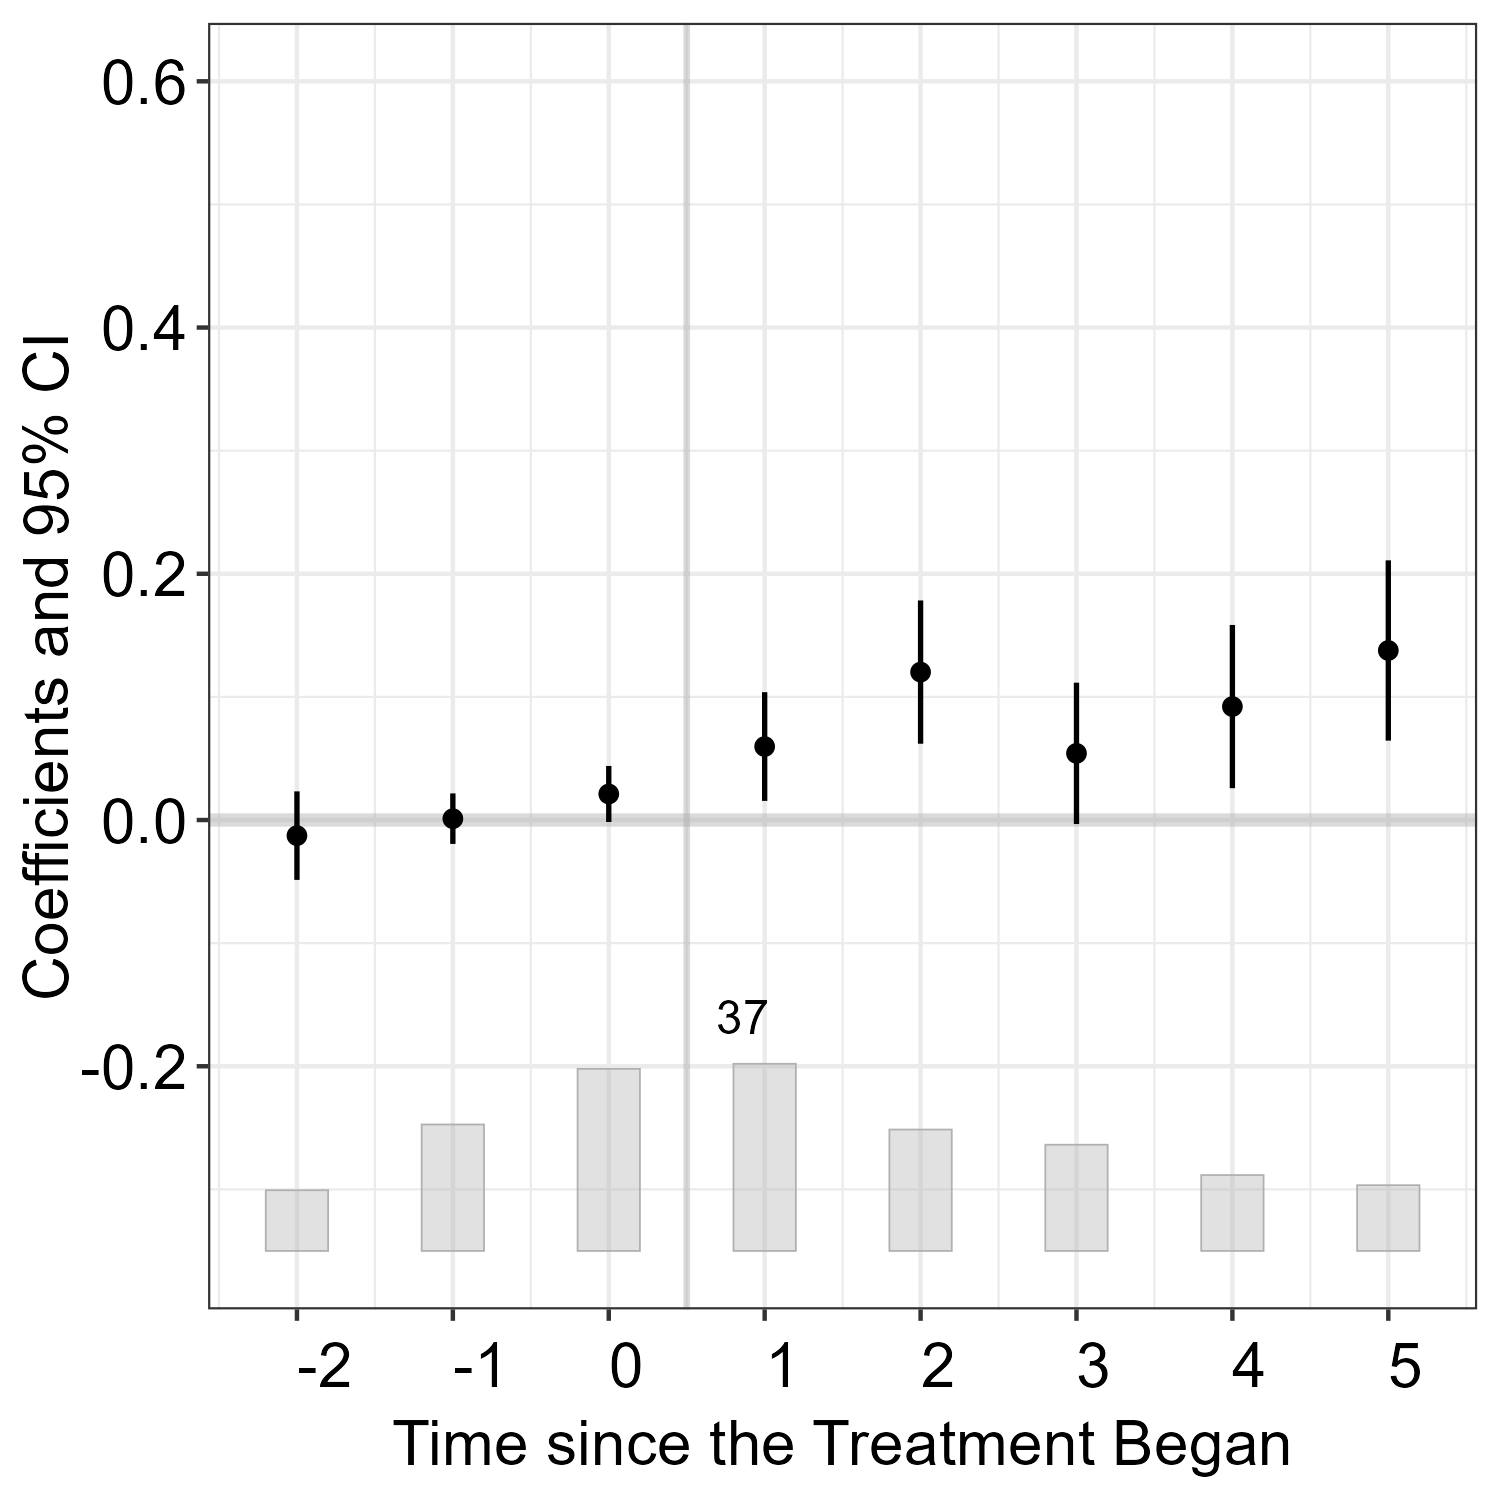
\includegraphics[width = 0.22\textwidth]{fect/Clark_fect_entry} \\ \\ 
    \citet{Clayton2018} \newline  ATT: 0.19 (0.44); \newline $p$-values: 0.09, 0.99 &
   \citet{cox2021budgetary} \newline  ATT: 0.44 (0.07); \newline $p$-values: 0.10, 0.00 &
   \citet{Distelhorst2018} \newline ATT: 0.15 (0.05); \newline $p$-values: 0.32, 0.00 & 
   \citet{eckhouse2022metrics} \newline ATT: 0.01 (0.01); \newline $p$-values: 0.40, 0.14 \\
   \hspace{-2em}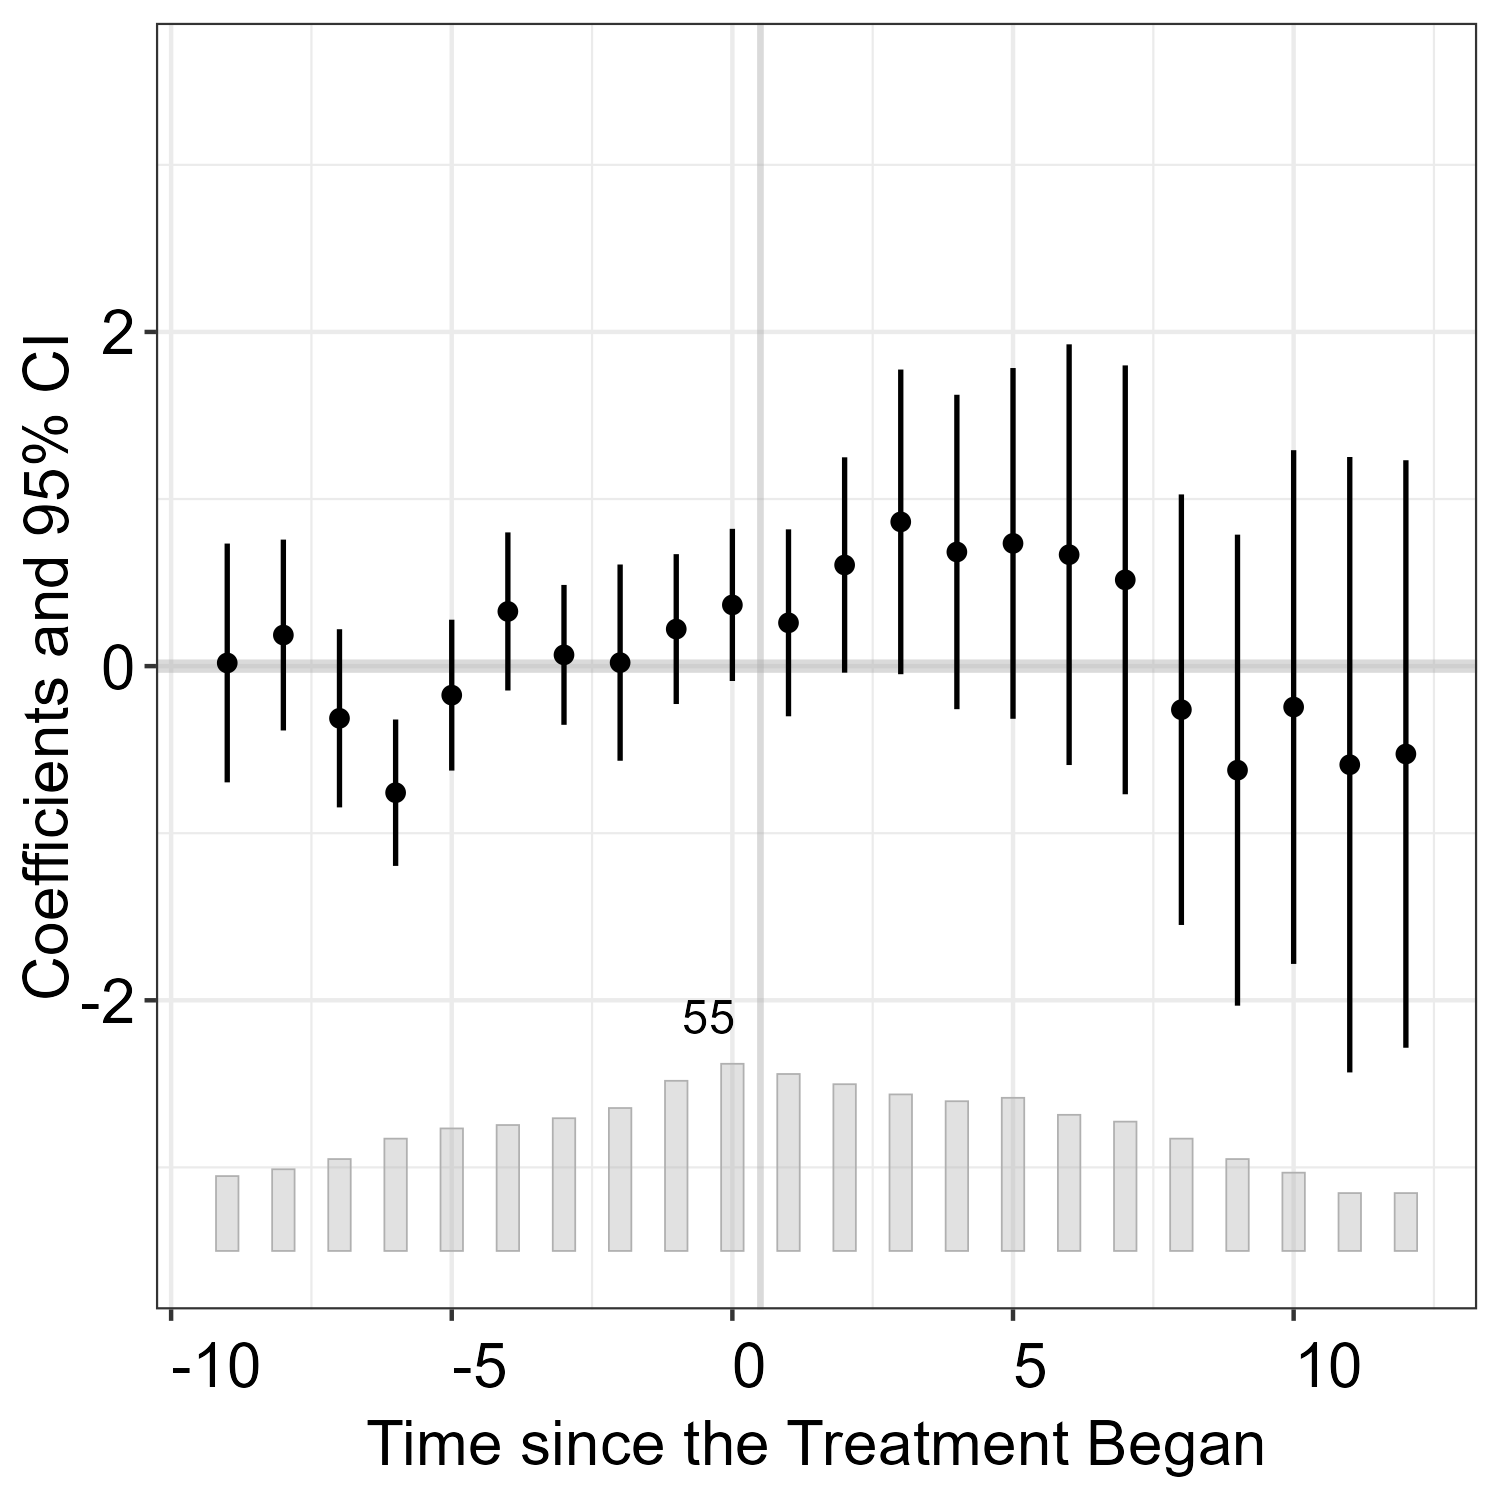
\includegraphics[width = 0.22\textwidth]{figure/fect/clayton_fect_entry.png} &
   \hspace{-2em} 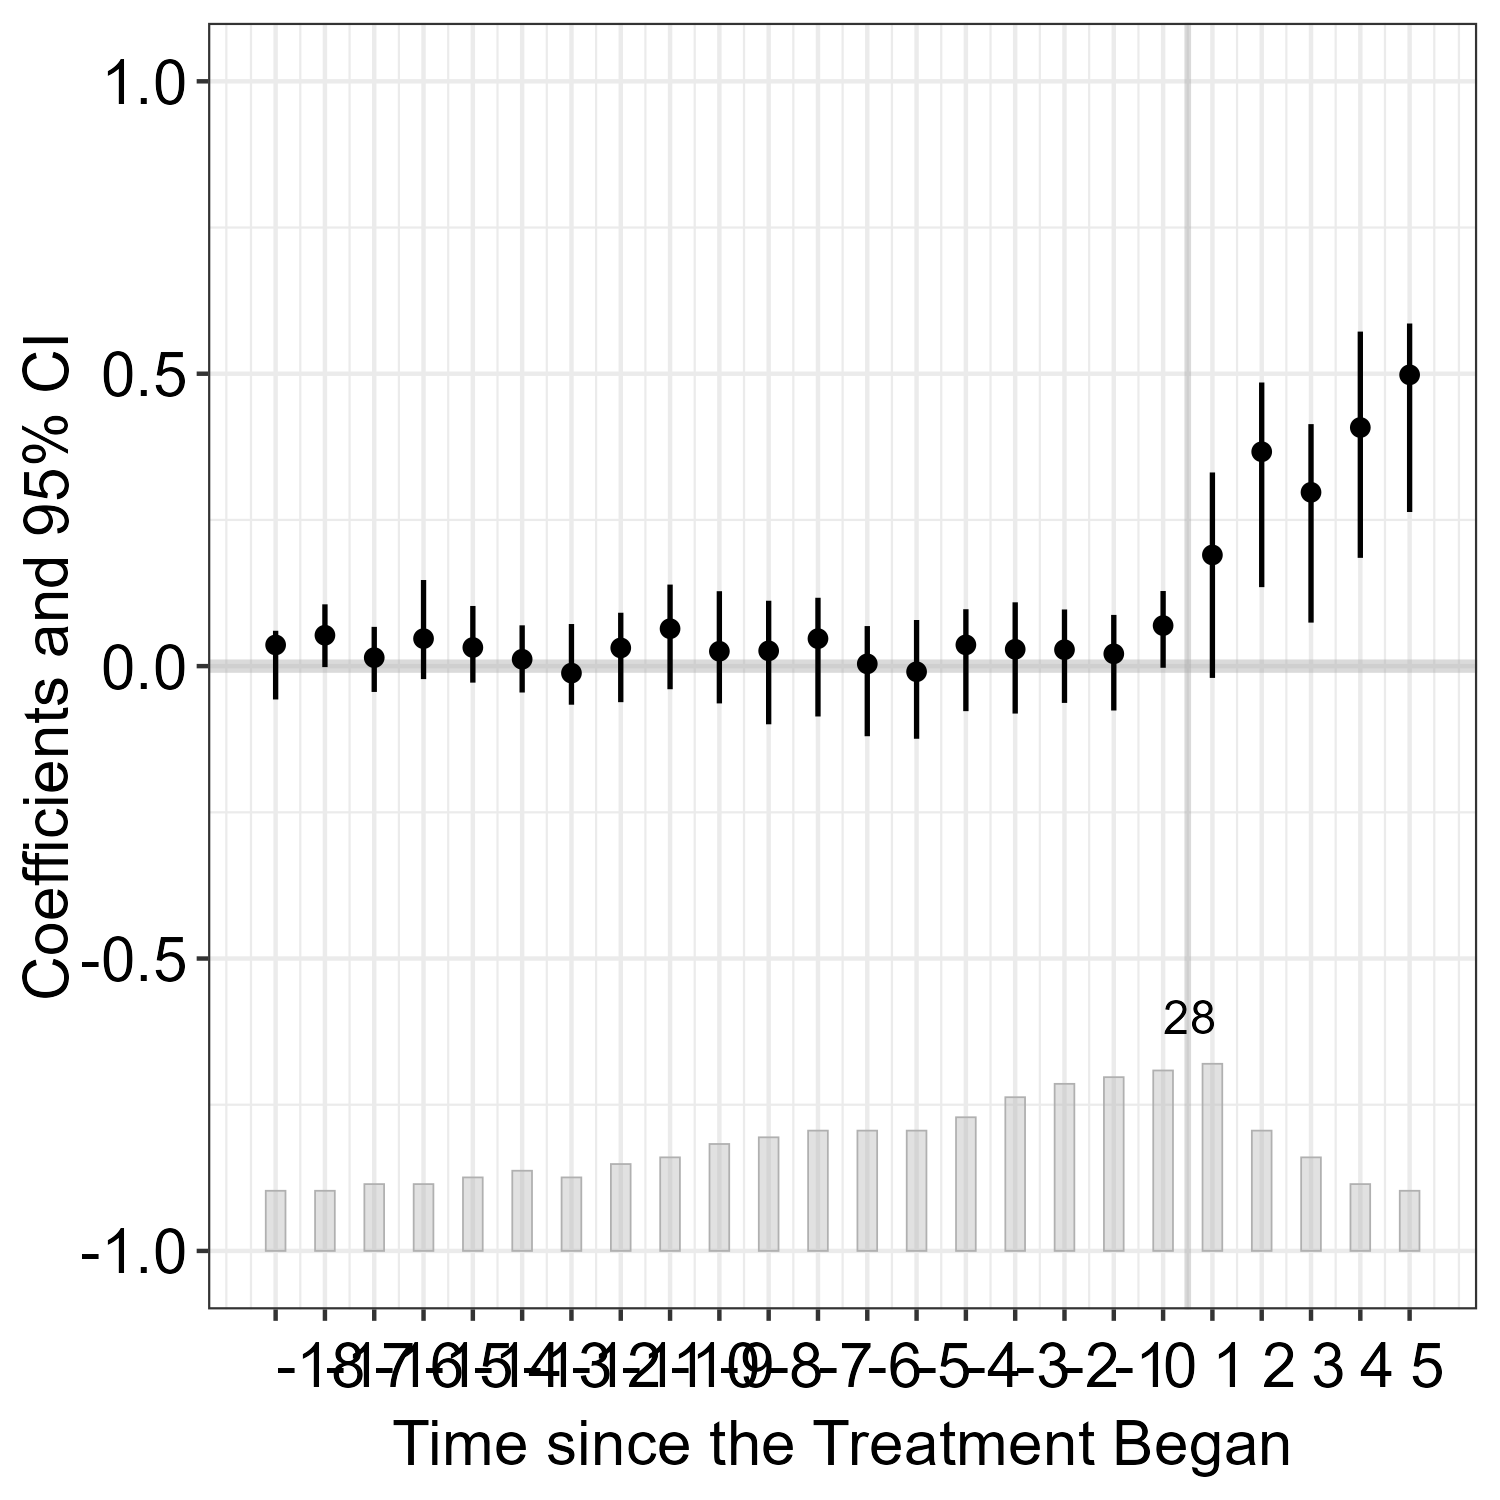
\includegraphics[width = 0.22\textwidth]{figure/fect/Cox_fect_entry.png} &
   \hspace{-2em}\includegraphics[width = 0.22\textwidth]{figure/fect/distelhorst_fect_entry} &
    \hspace{-2em} 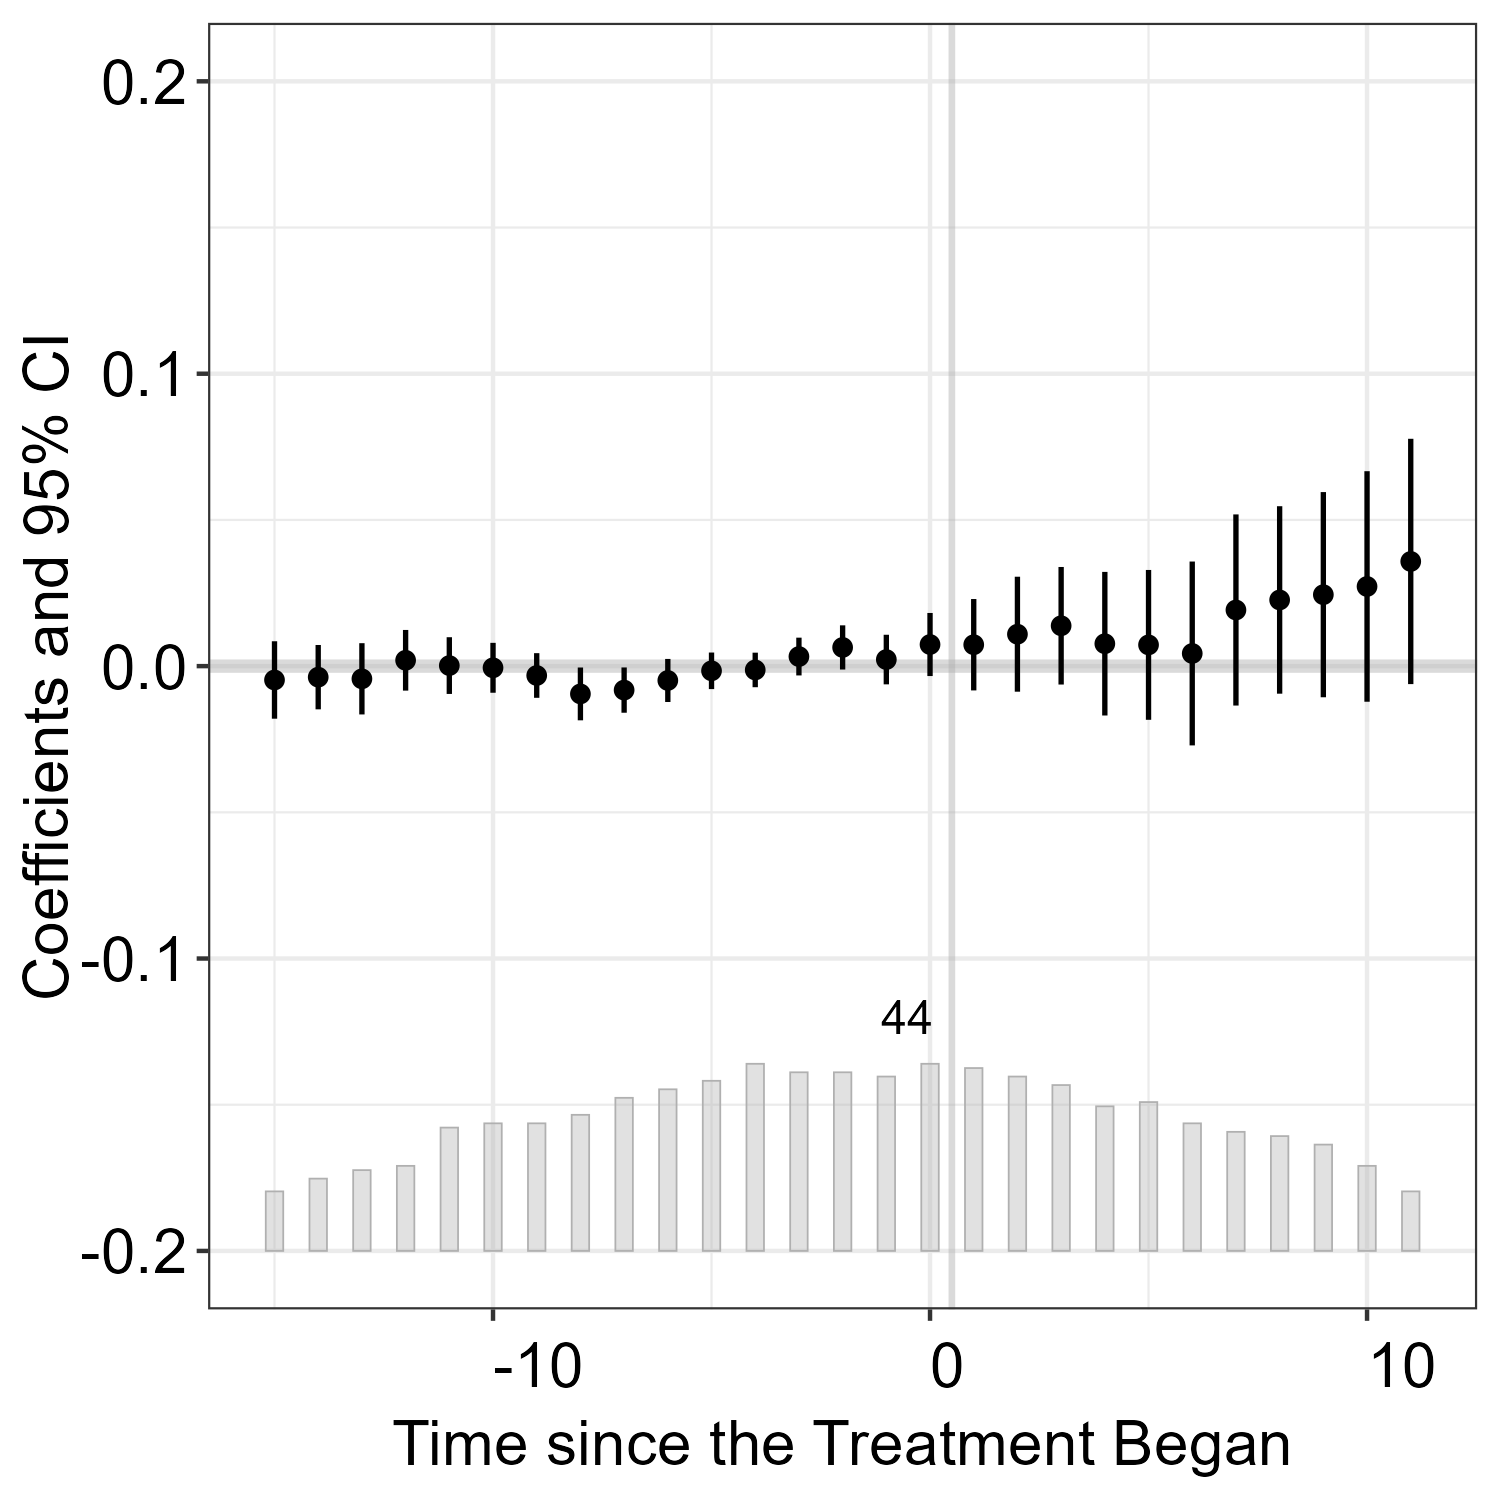
\includegraphics[width = 0.22\textwidth]{figure/fect/eckhouse_fect_entry.png}\\ \\ 
   \citet{Fouirnaies2018ajps} \newline ATT:  0.87 (0.11); \newline $p$-values: 0.00, 0.00 &
   \citet{fh2018} \newline ATT:  0.29 (0.02); \newline $p$-values: 0.21, 0.00 &
   \citet{Fouirnaies2022} \newline ATT:-0.26 (0.03); \newline $p$-values: 0.00, 0.00 & 
    \citet{Fresh2018} \newline  ATT: 0.17 (0.06); \newline $p$-values: 0.85, 0.000\\   
   \hspace{-2em} 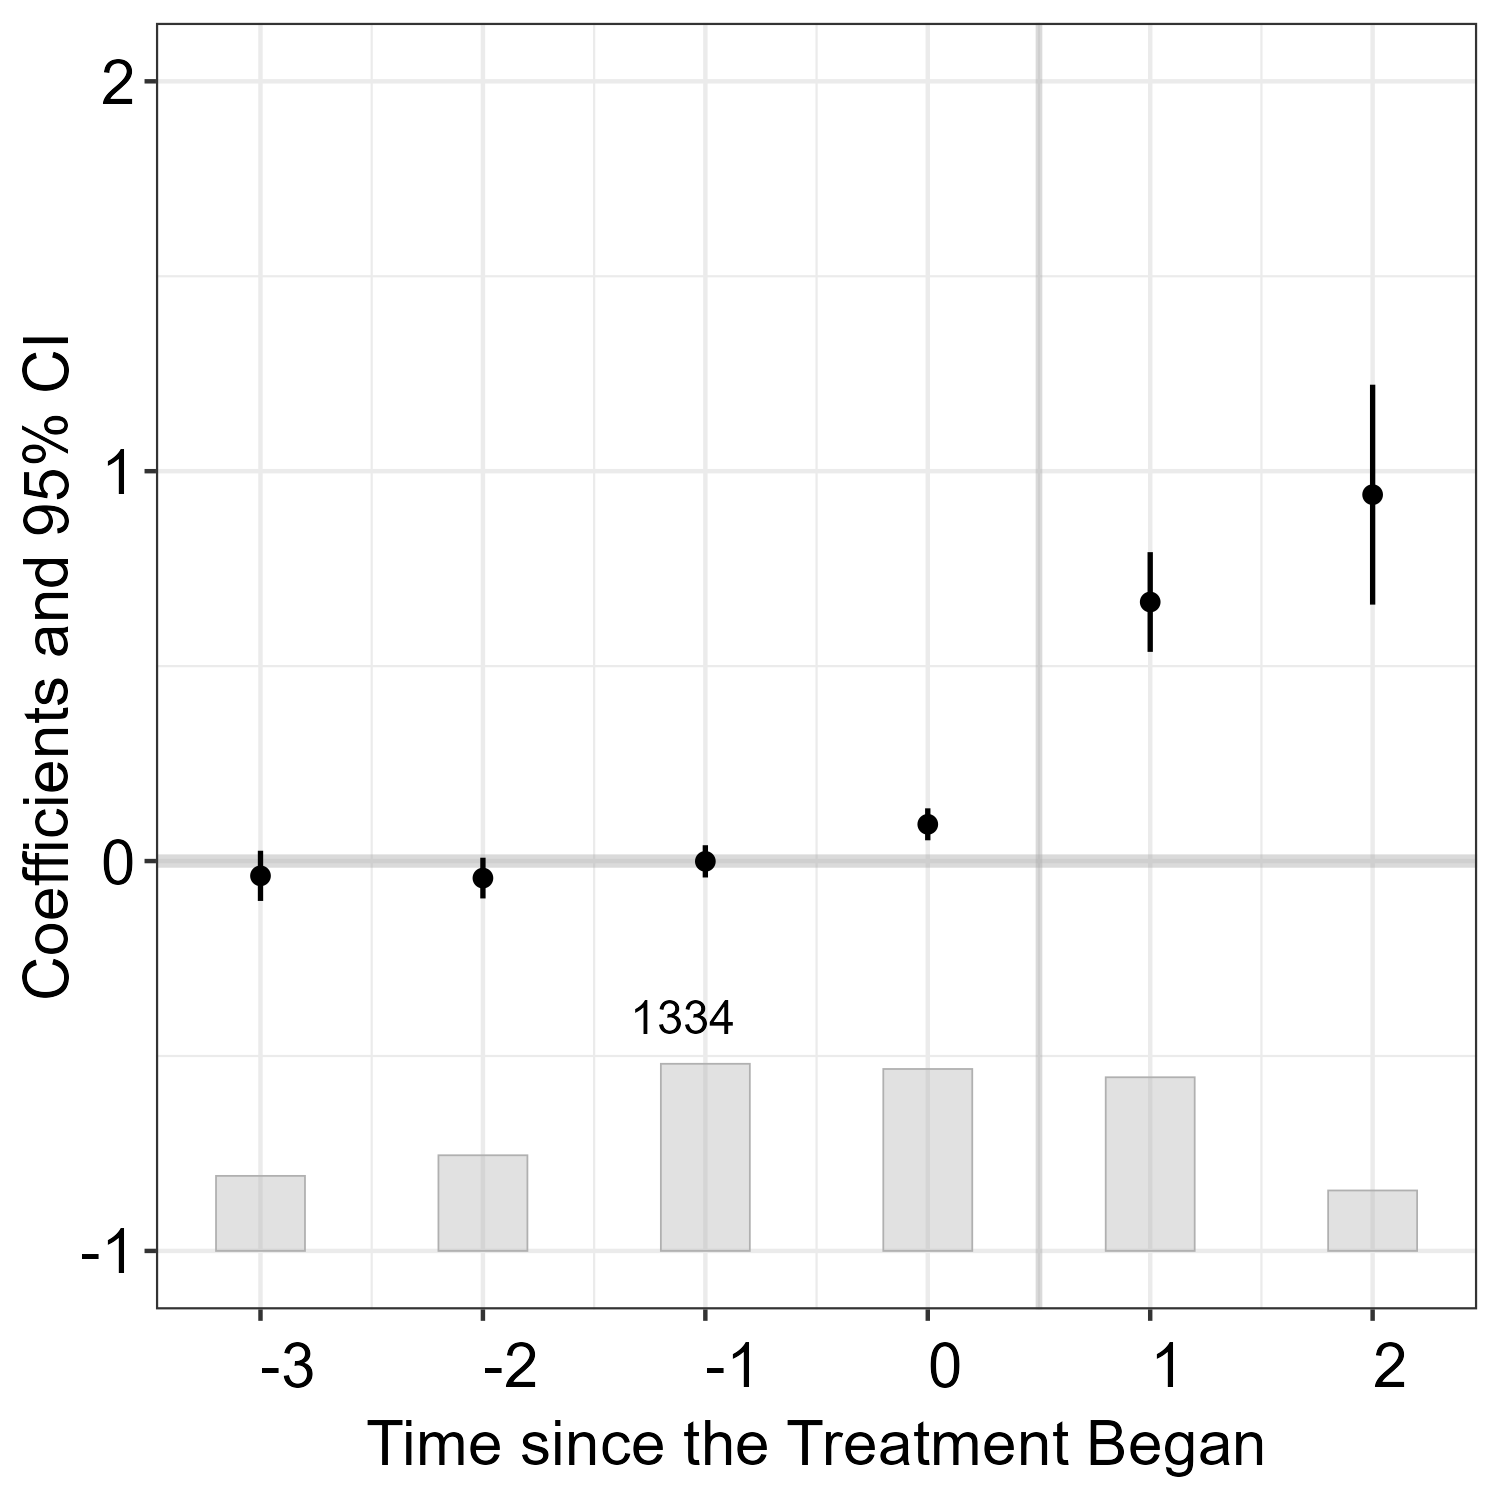
\includegraphics[width = 0.22\textwidth]{figure/fect/Fouirnaies_fect_entry.png} &
   \hspace{-2em}  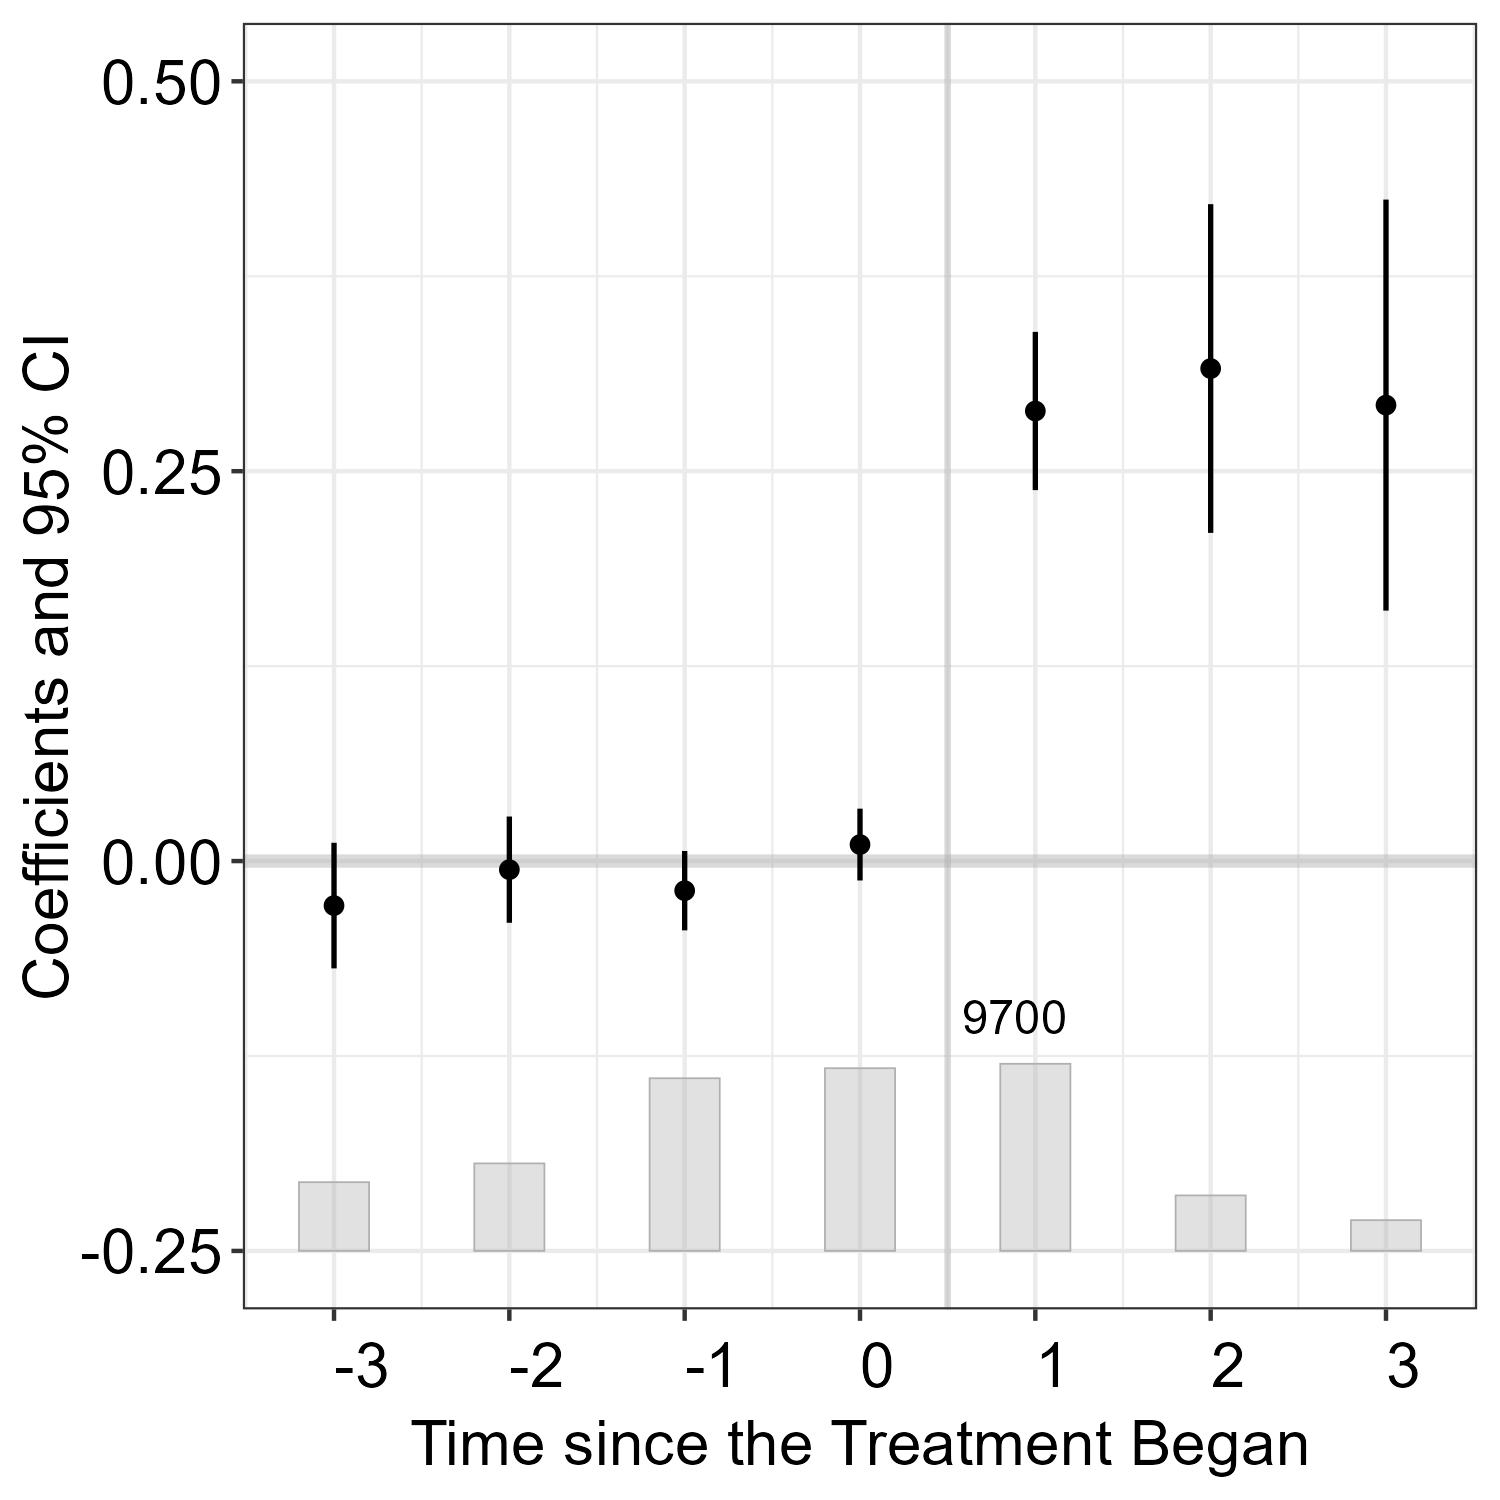
\includegraphics[width = 0.22\textwidth]{figure/fect/FouirnaiesHall_fect_entry.png} & 
   \hspace{-2em} 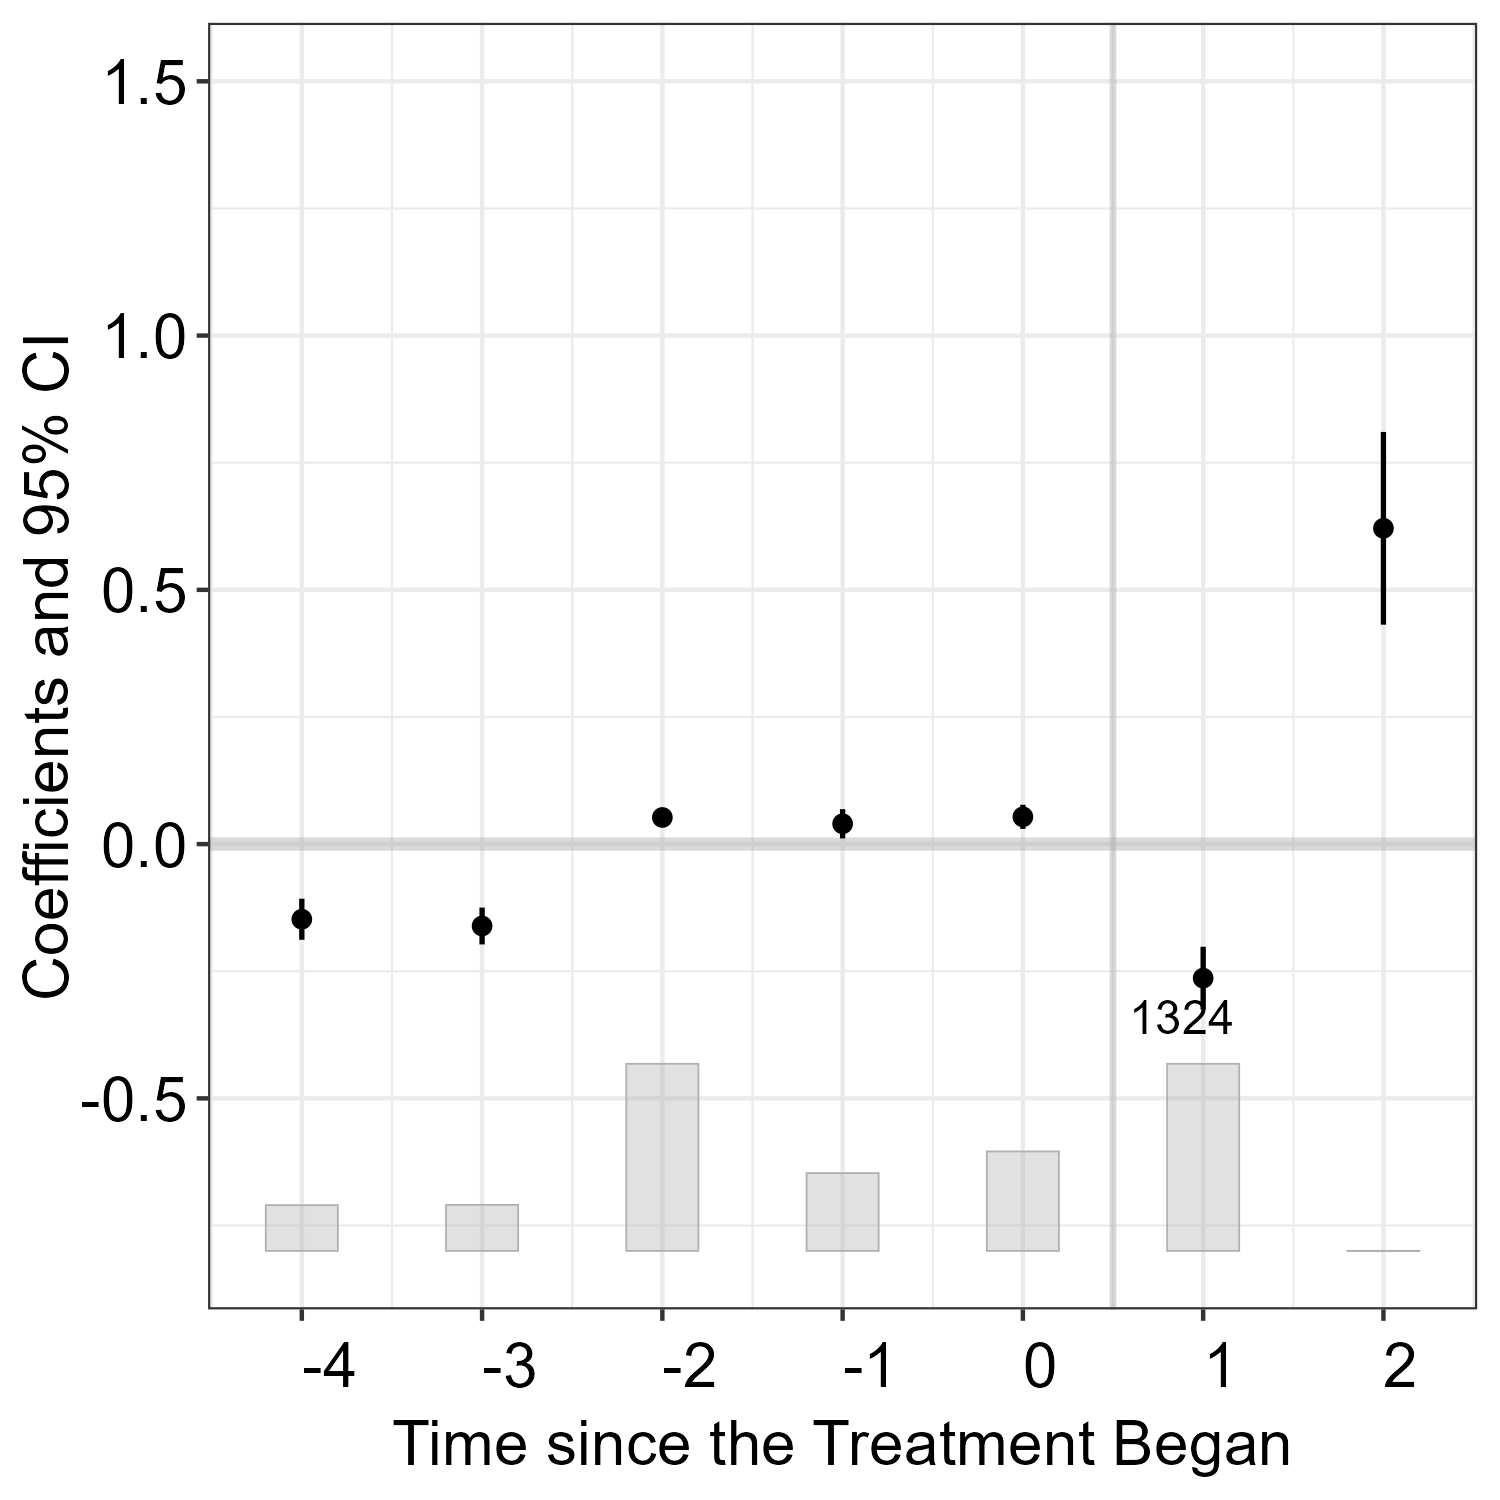
\includegraphics[width = 0.22\textwidth]{figure/fect/Fouirnaies2022_fect_entry.png}  &
    \hspace{-2em}  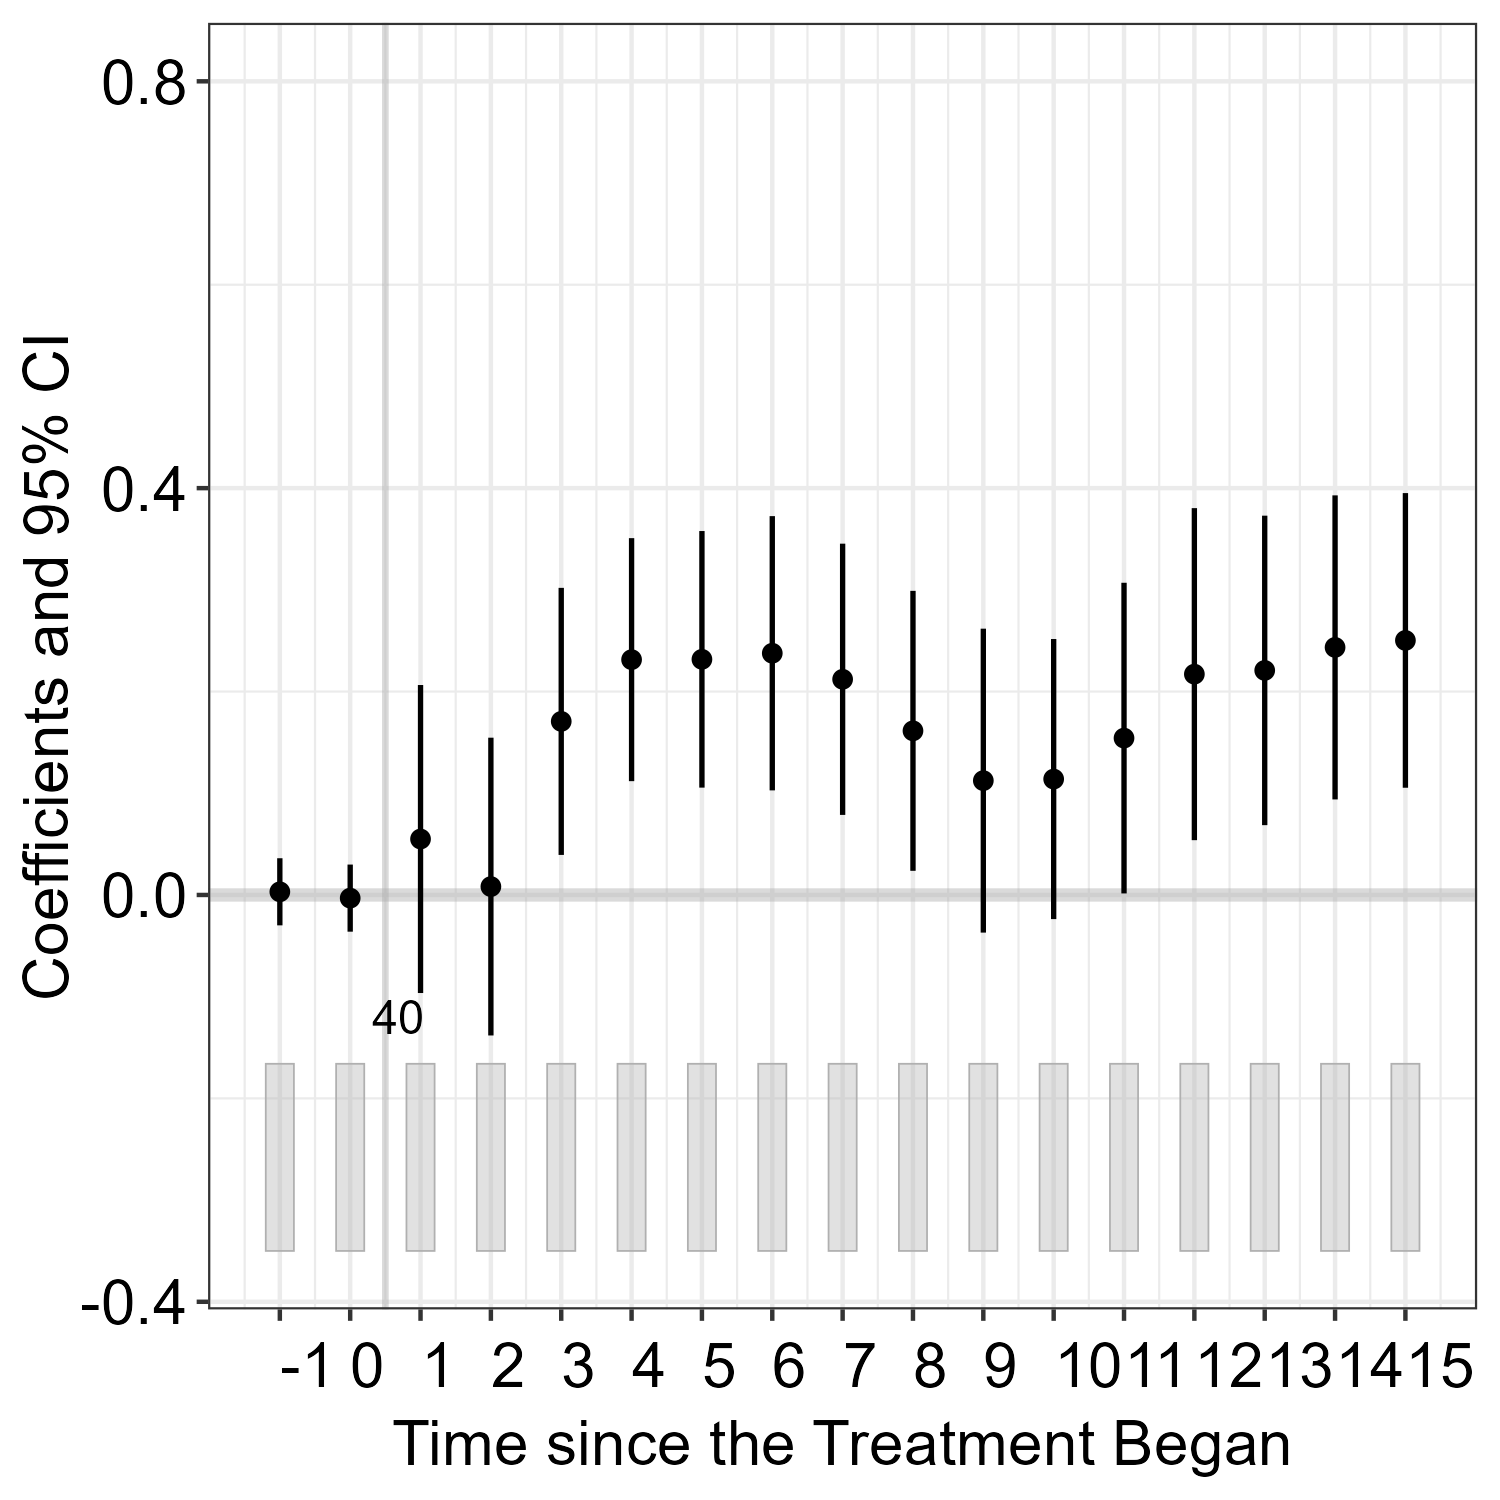
\includegraphics[width = 0.22\textwidth]{figure/fect/Fresh_fect_entry.png}\\ \\ 
   \citet{Garfias2019jop} \newline  ATT: 0.07 (0.03); \newline $p$-values: 0.90, 0.42  &   
   \citet{Grumbach2020}\newline  ATT: 0.13 (0.03); \newline $p$-values: 0.42, 0.00 &
   \citet{Grumbach2022} \newline  ATT: 0.033 (0.018); \newline $p$-values: 0.86, 0.37  &
      \citet{hainmueller2019does} \newline  ATT: 1.51 (0.21); \newline $p$-values: 0.08, 0.00\\  
   \hspace{-2em}  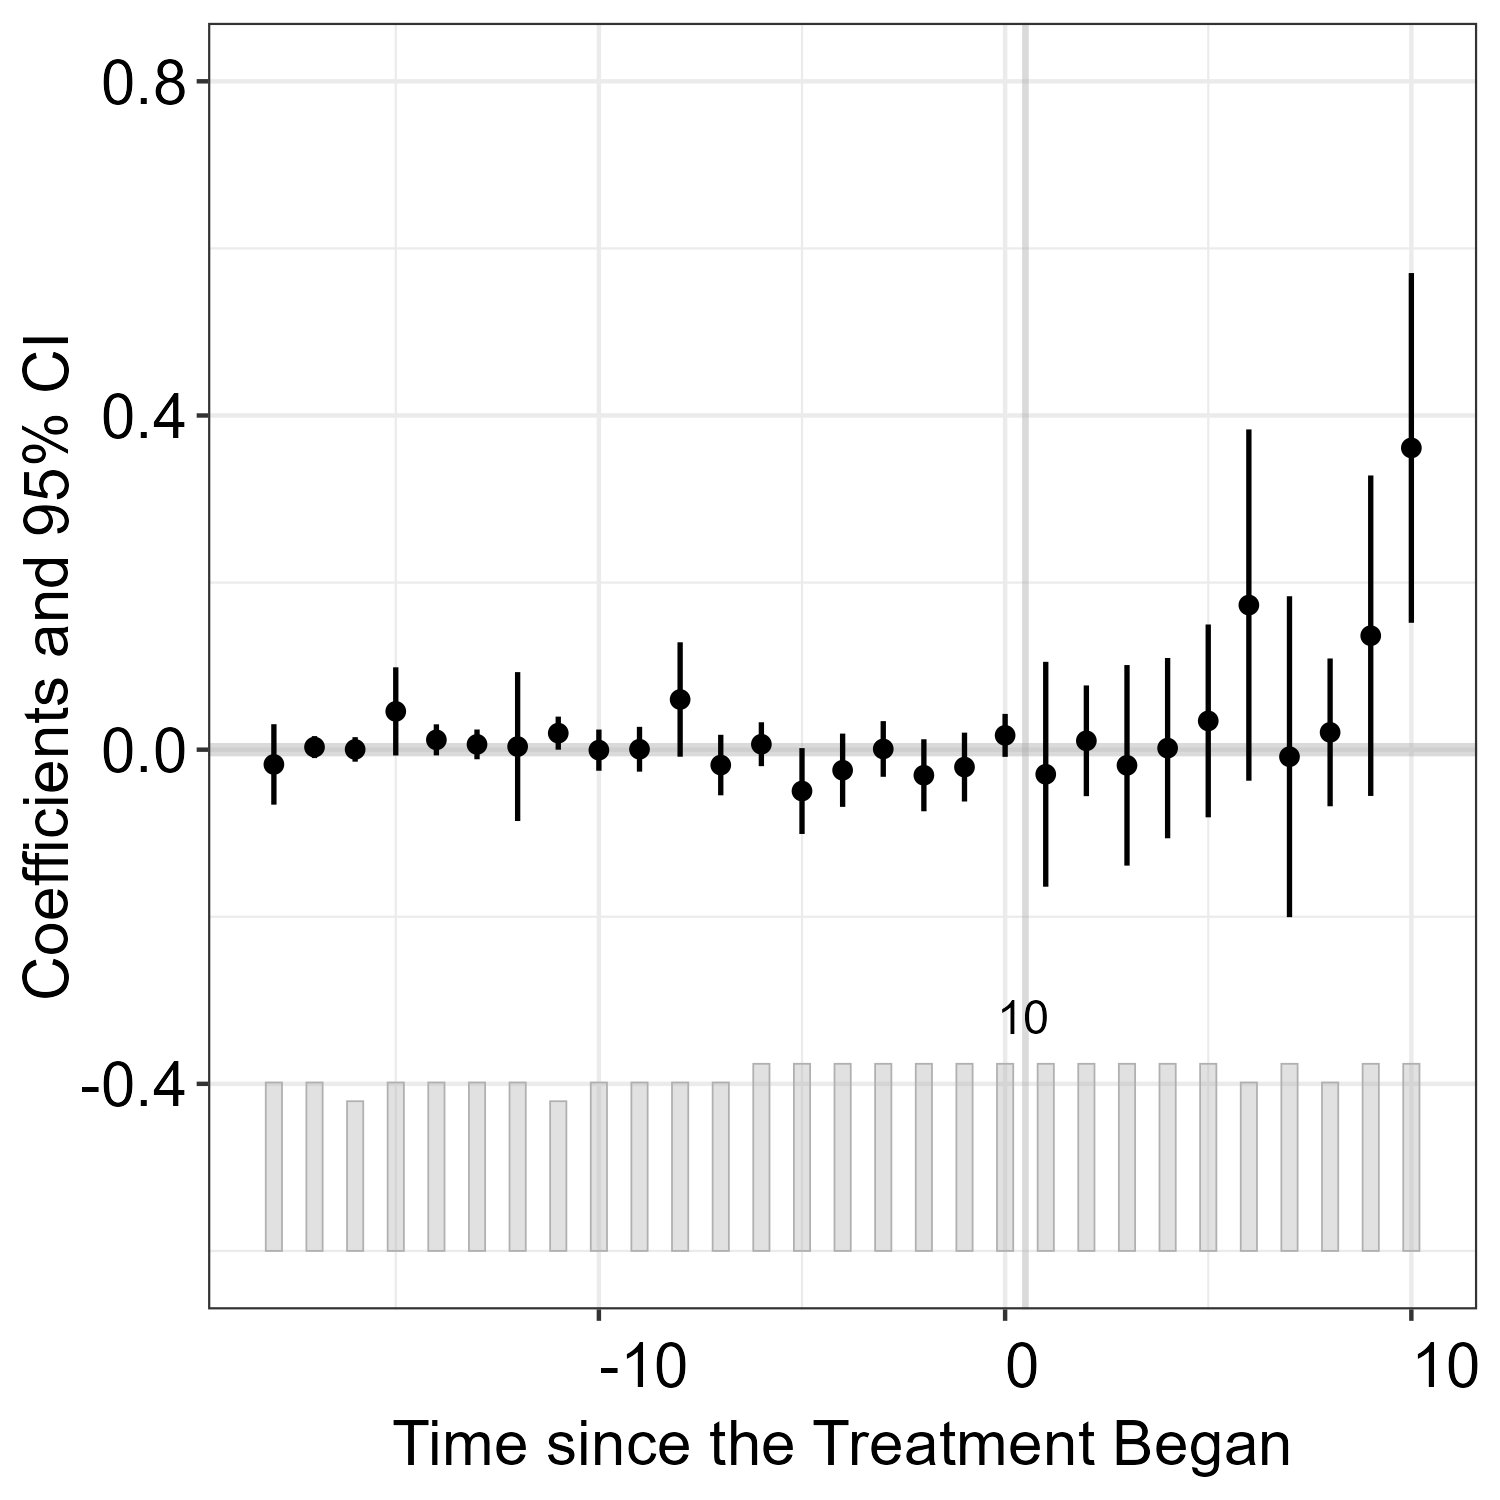
\includegraphics[width = 0.22\textwidth]{figure/fect/garfias_fect_entry.png} &  
   \hspace{-2em}  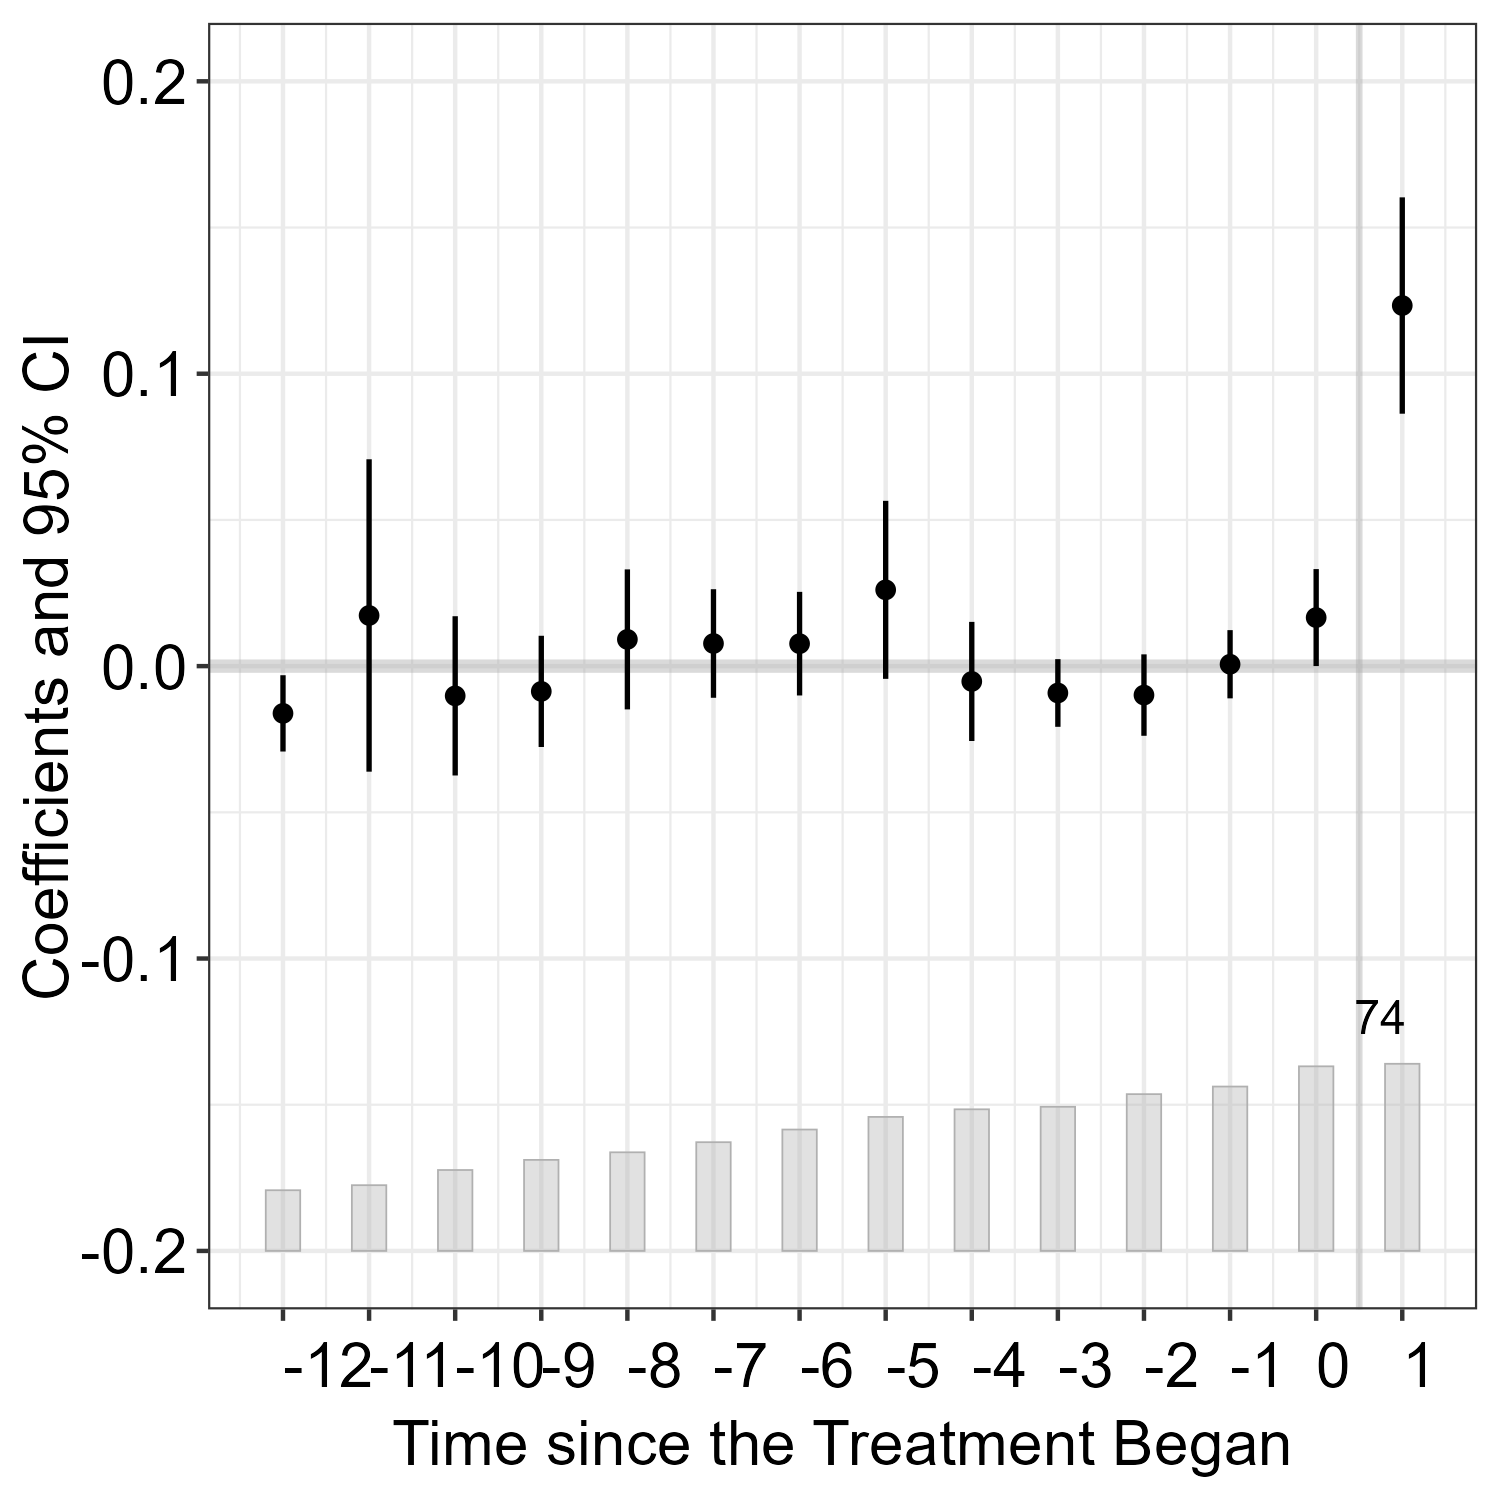
\includegraphics[width = 0.22\textwidth]{figure/fect/Grumbach_fect_entry.png} &
   \hspace{-2em}  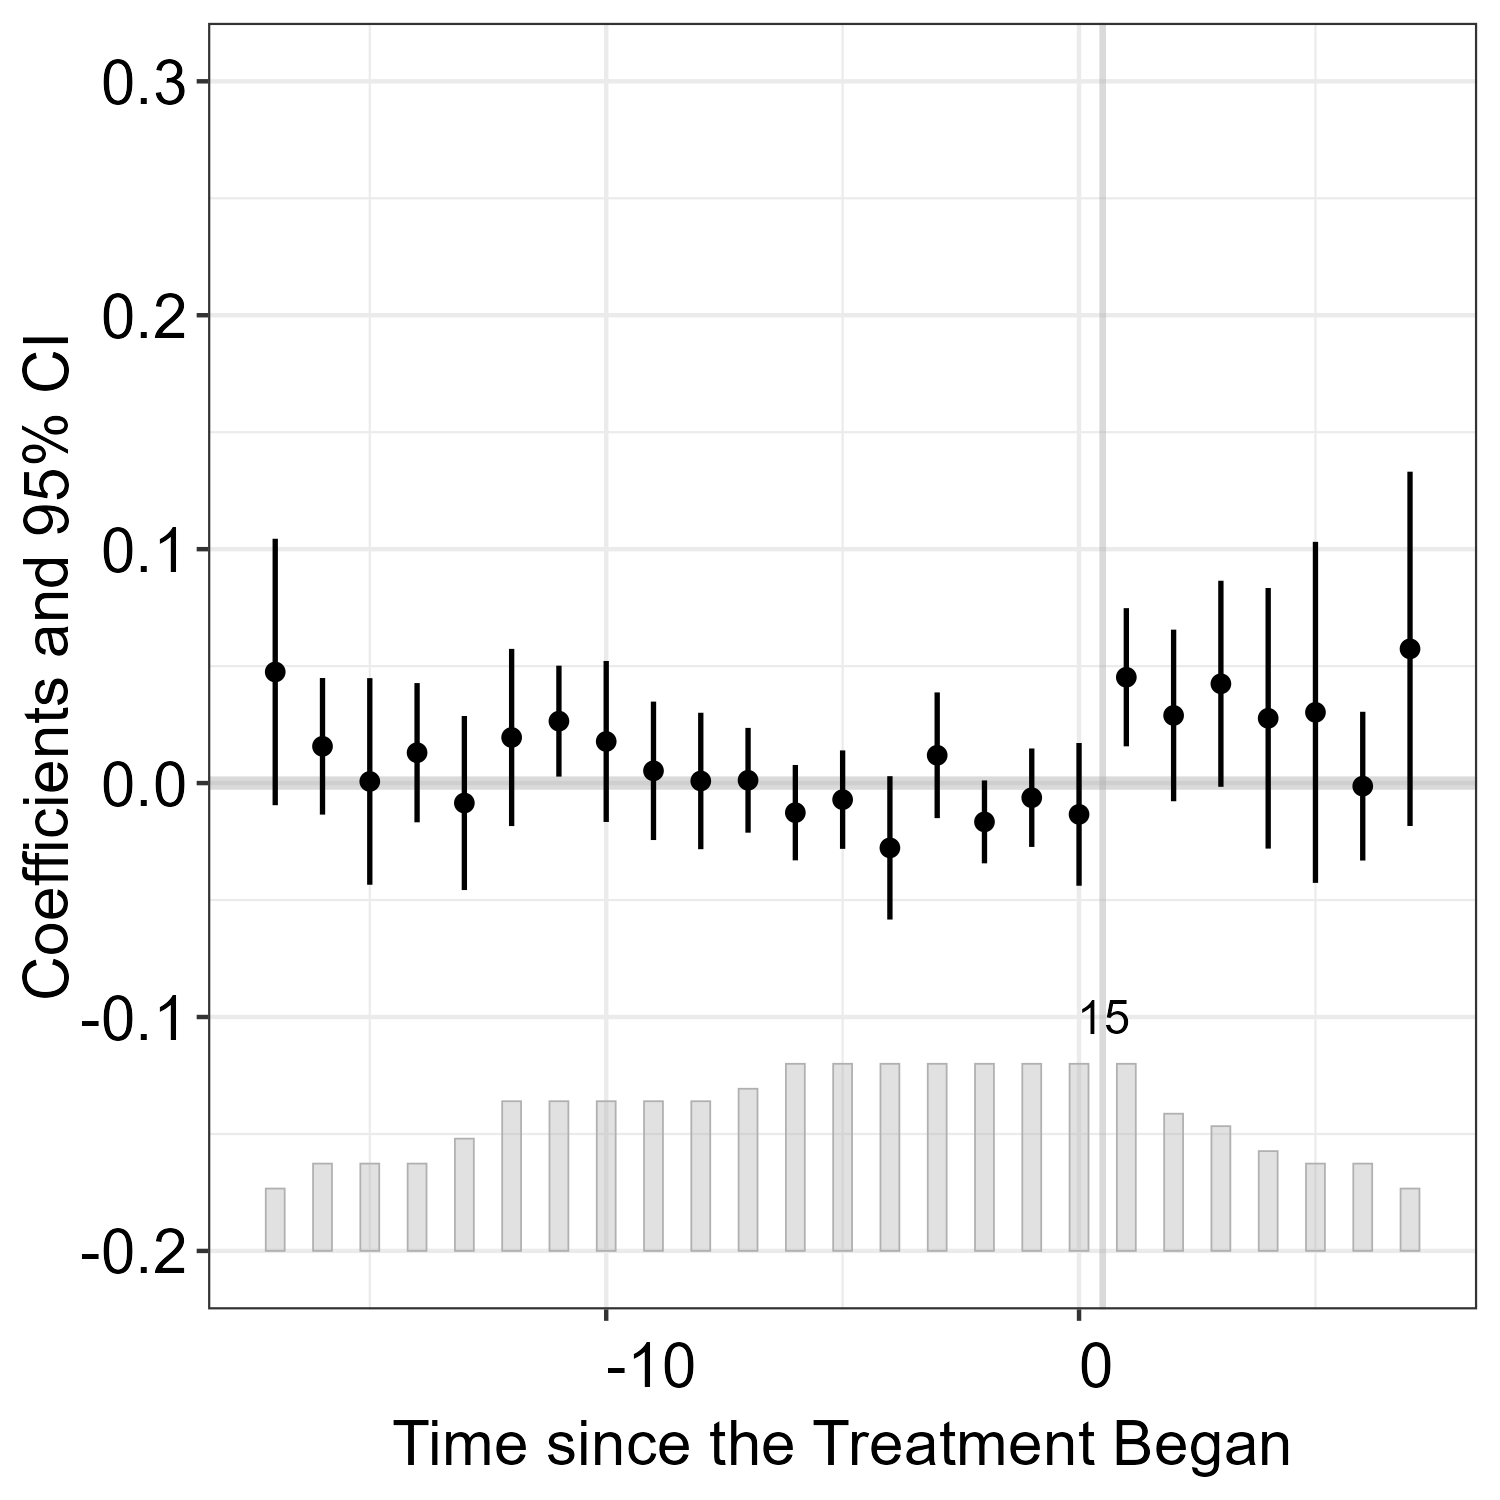
\includegraphics[width = 0.22\textwidth]{figure/fect/GH_fect_entry.png}  &
   \hspace{-2em}  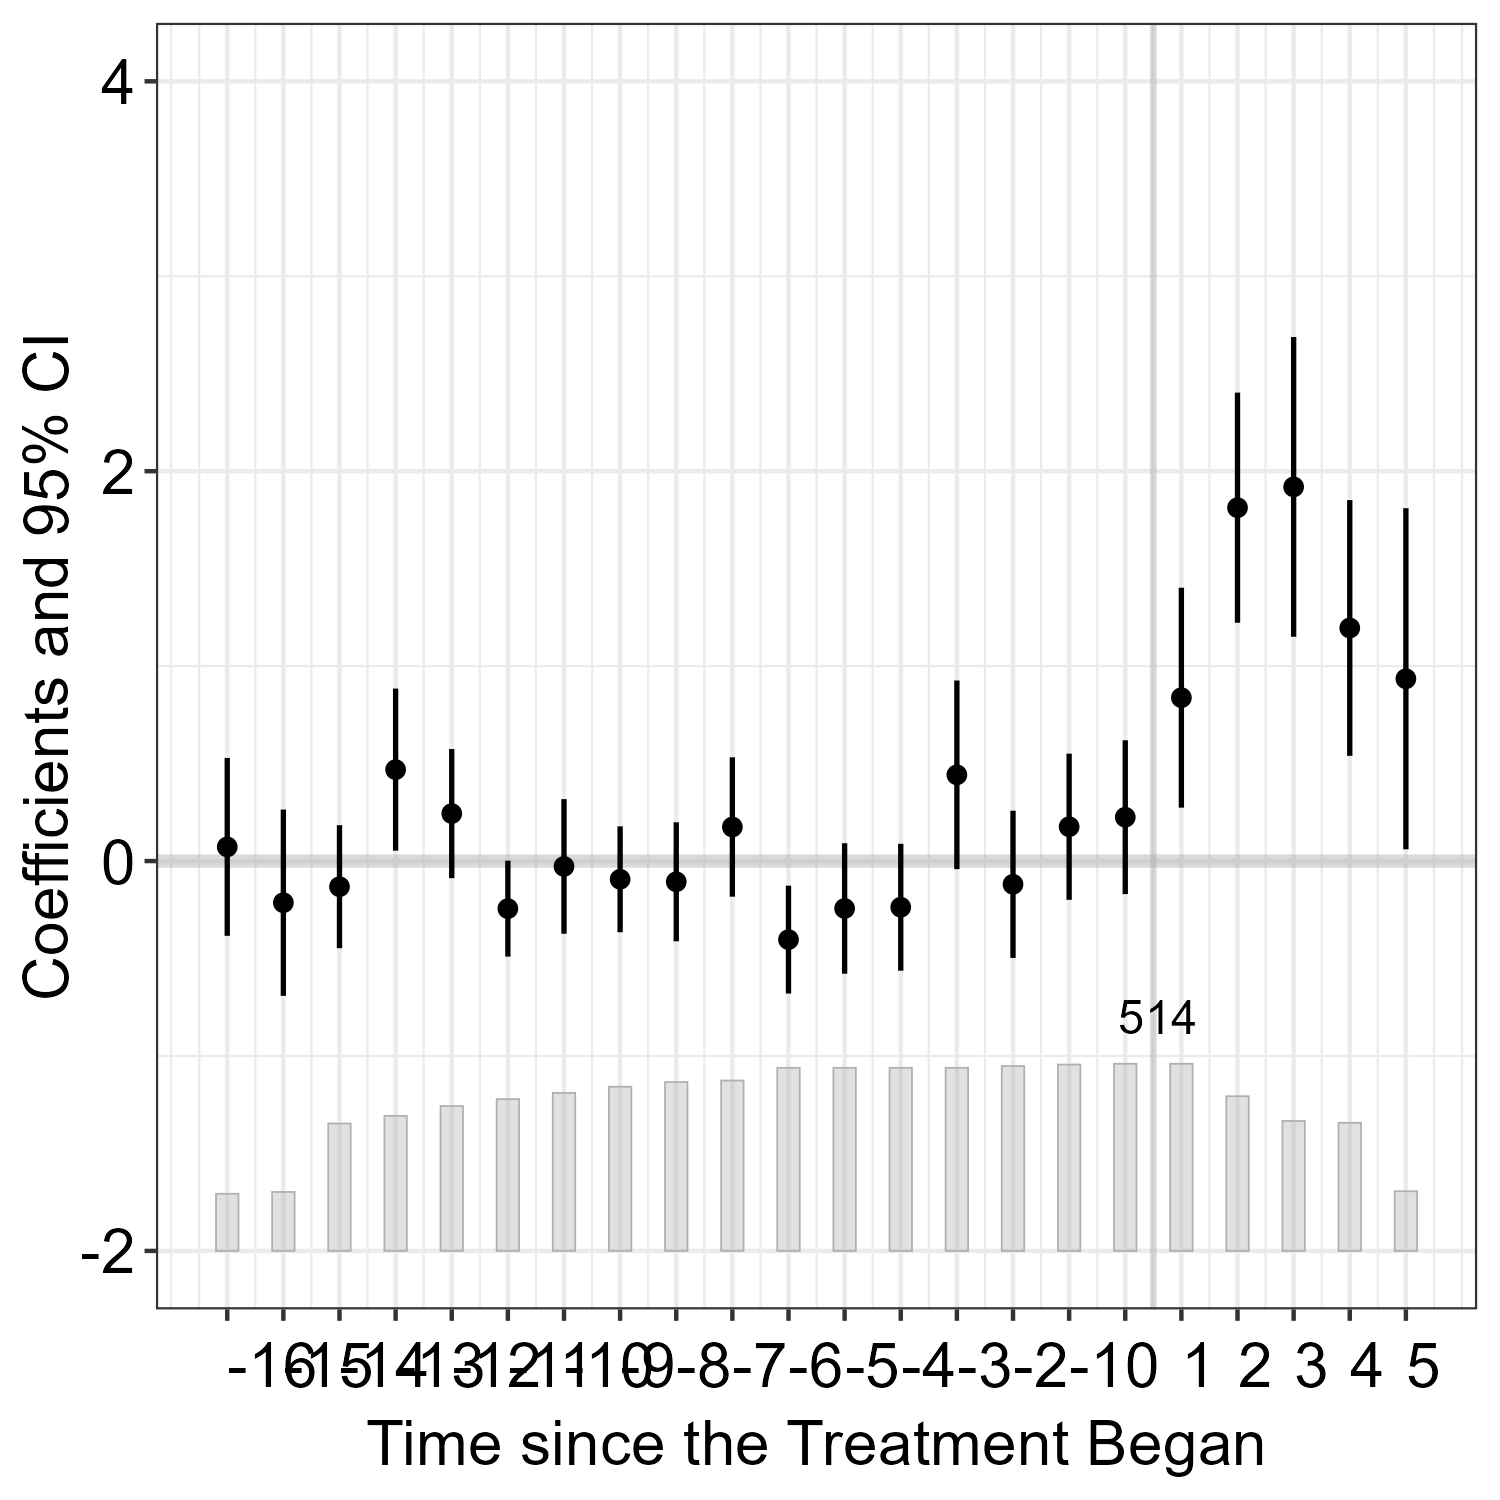
\includegraphics[width = 0.22\textwidth]{figure/fect/Hainmueller_fect_entry.png}\\ \\
\end{tabular}}
}
\end{minipage}\vspace{-0.5em}
\addtocounter{figure}{-1}
\end{figure}


\begin{figure}[!ht]
\caption{Estimated Dynamic Treatment Effects (Cont.)}
\centering\scriptsize
\begin{minipage}{1\linewidth}{
\centering
\hspace{1.5em}
\resizebox{0.9\textwidth}{!}{
\begin{tabular}{C{3.8cm}C{3.8cm}C{3.8cm}C{3.8cm}}
   \citet{Hall2022} \newline  ATT: 0.06 (0.003); \newline $p$-values: 0.00, 0.00 & 
   \citet{Hirano2022} \newline  ATT: 0.56 (0.18); \newline $p$-values: 0.20, 0.00 &
   \citet{Jiang2018} \newline  ATT: -0.87 (0.20); \newline $p$-values: 0.51, 0.00 &
   \citet{kilborn2022public} \newline ATT: 0.12 (0.04); \newline $p$-values: 0.90, 0.00\\ 
   \hspace{-2em}  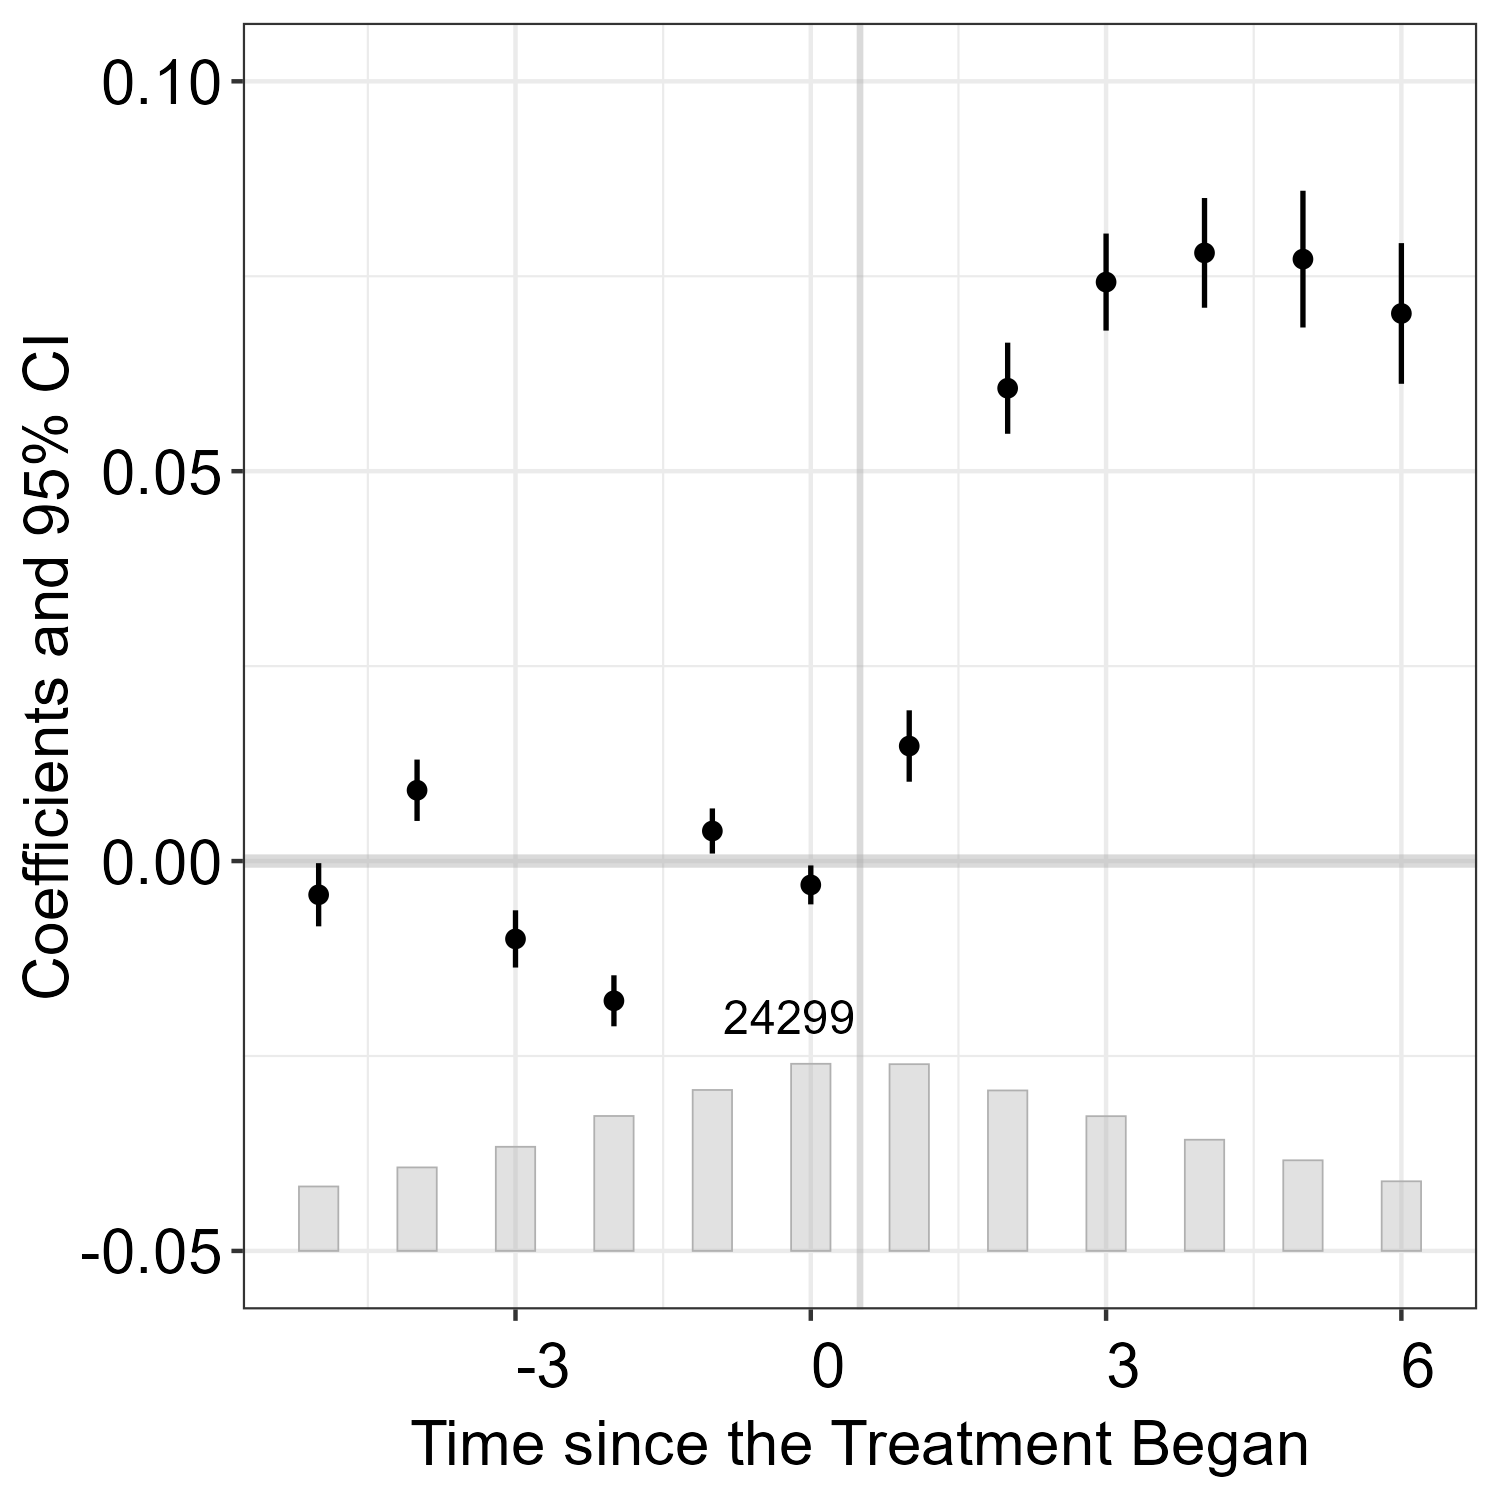
\includegraphics[width = 0.22\textwidth]{figure/fect/hallyoder_fect_entry.png}  &
   \hspace{-2em} 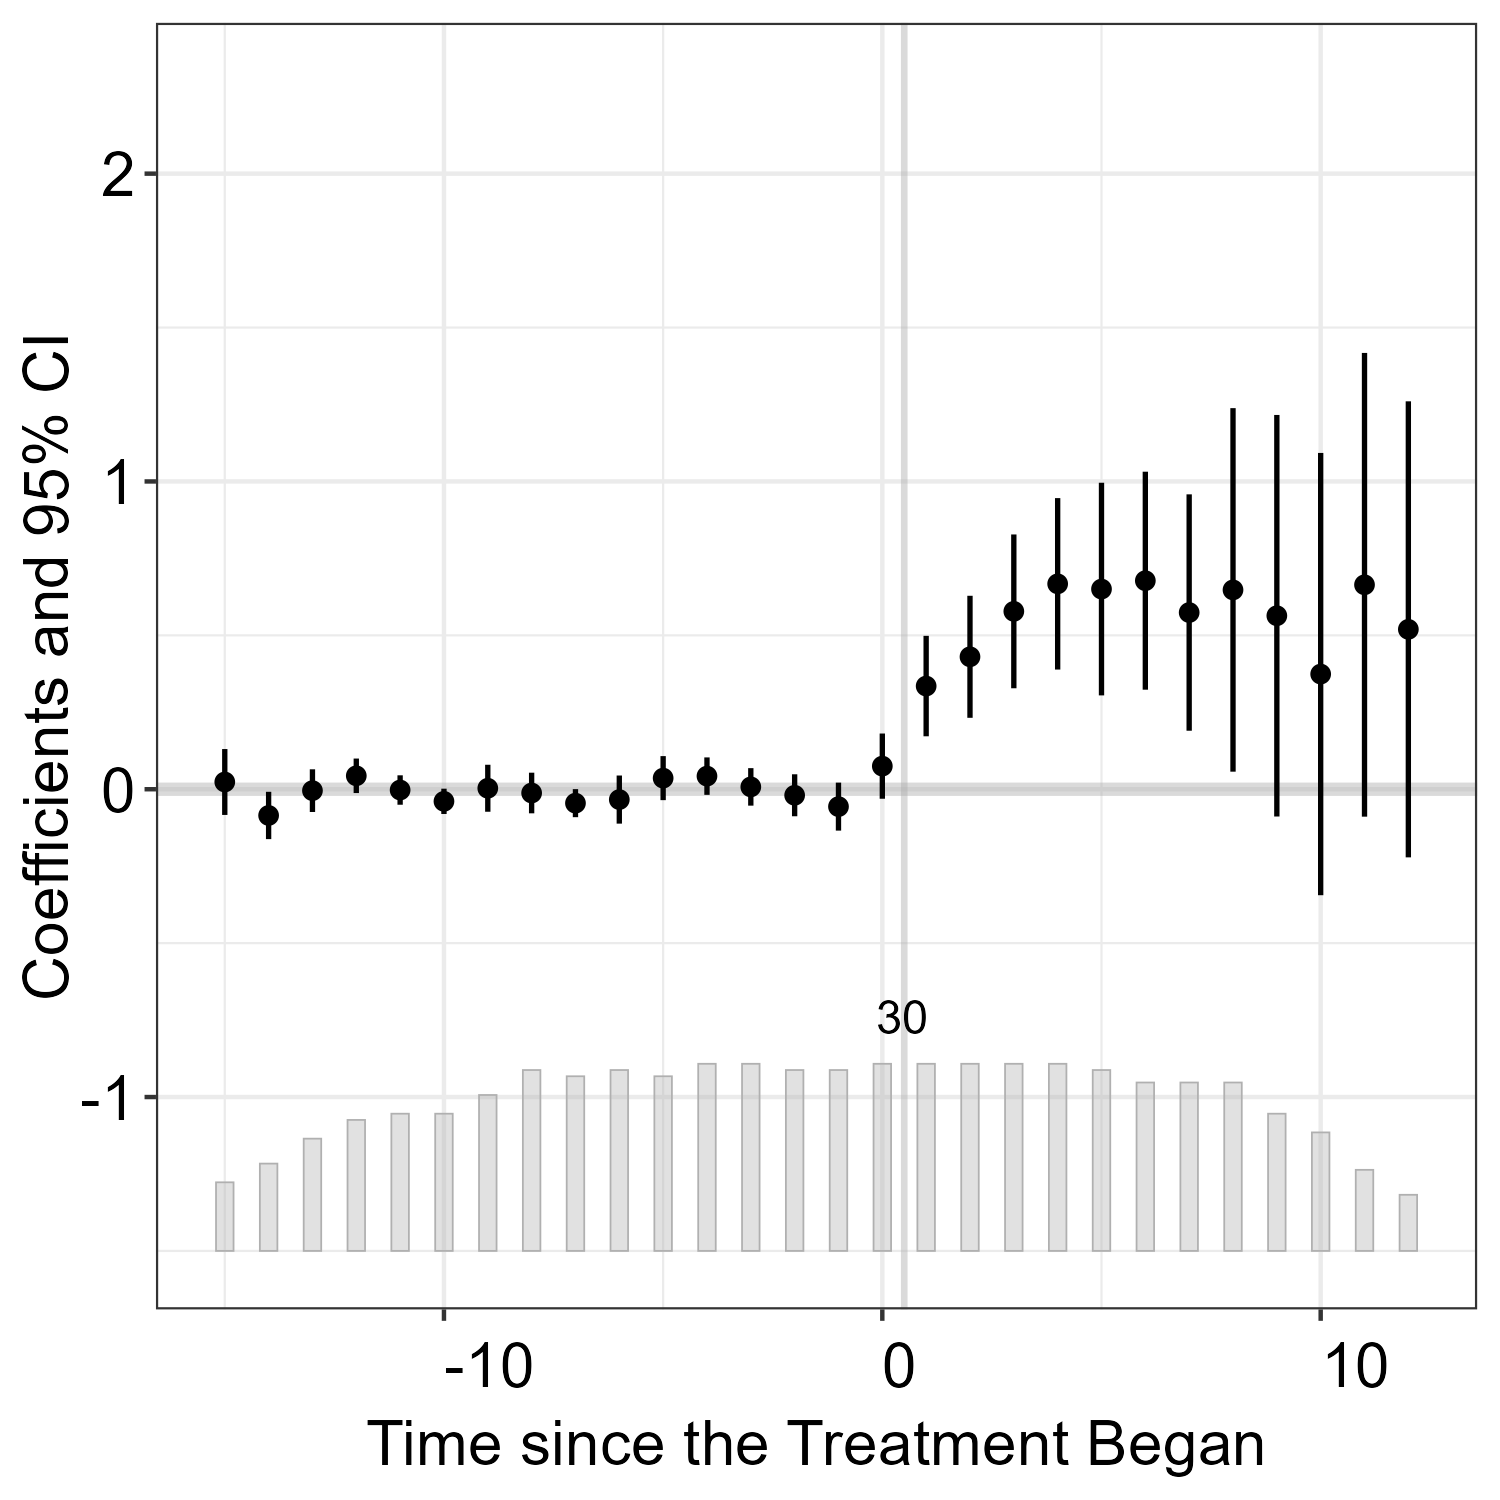
\includegraphics[width = 0.22\textwidth]{figure/fect/hirano_fect_entry.png}  &
   \hspace{-2em} 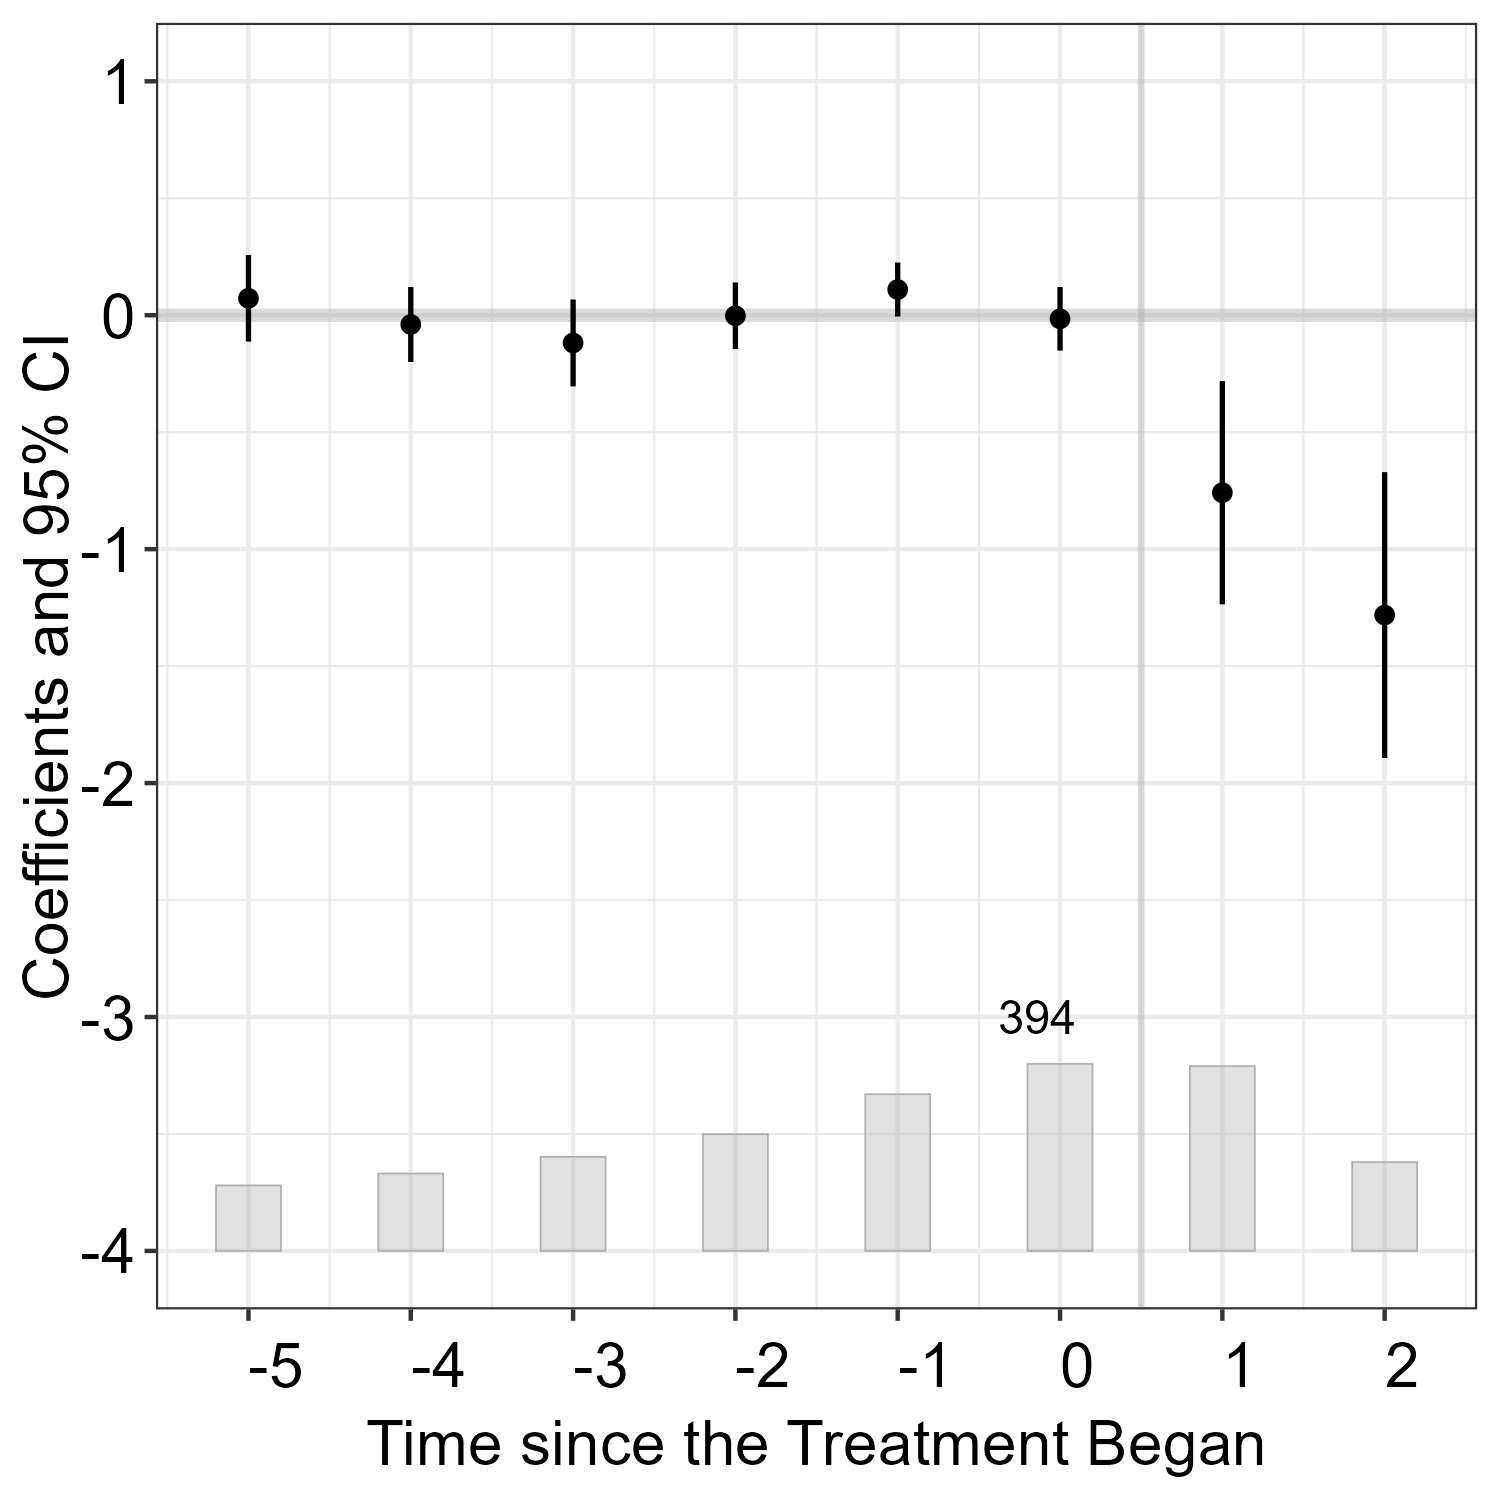
\includegraphics[width = 0.22\textwidth]{figure/fect/jiang_fect_entry.png}  &
   \hspace{-2em}  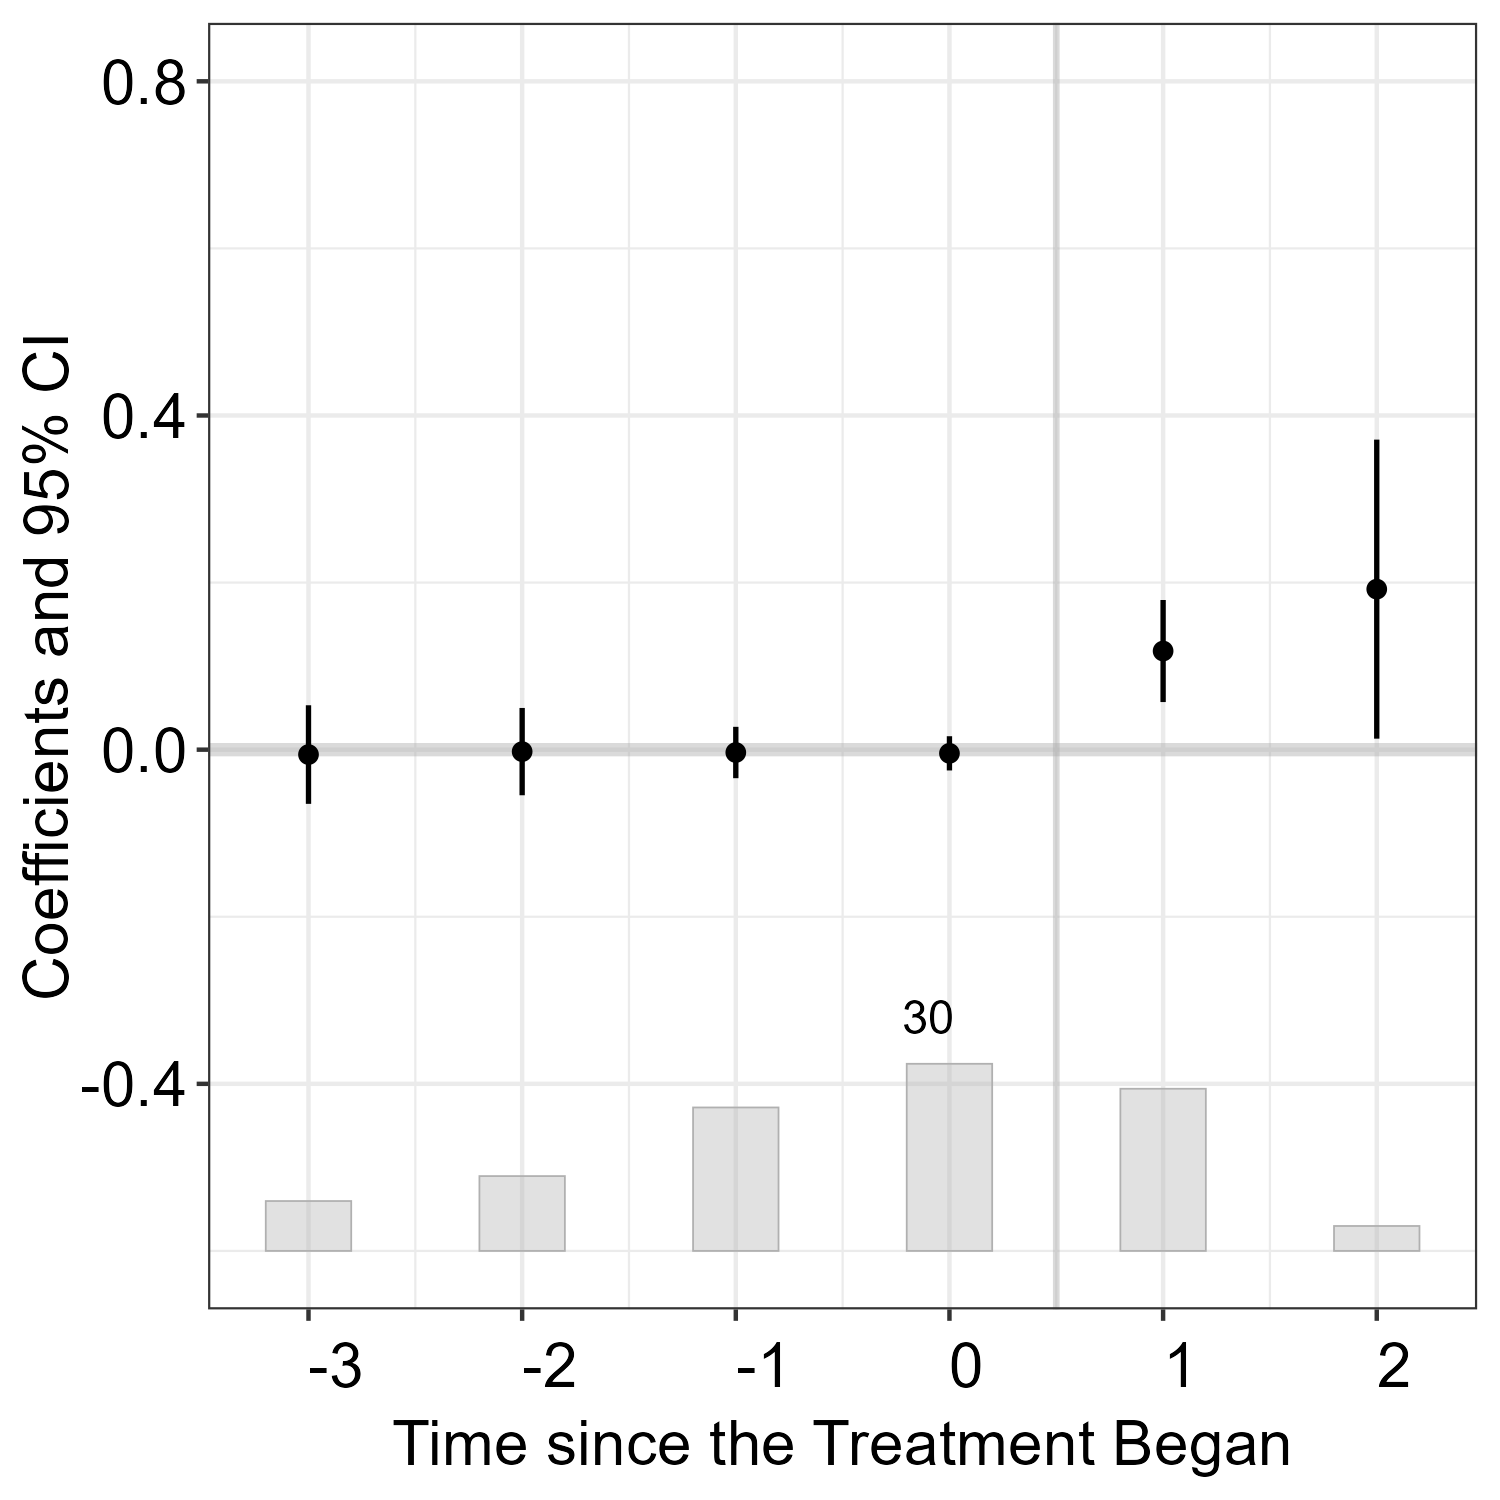
\includegraphics[width = 0.22\textwidth]{figure/fect/kilborn_fect_entry.png}\\ \\ 
   \citet{Kogan2021} \newline  ATT: 0.45 (0.39); \newline $p$-values: 0.85, 0.00 & 
   \citet{magaloni2020killing} \newline  ATT: -2.28 (0.96); \newline $p$-values: 0.59, 0.02 &
   \citet{Paglayan2022} \newline  ATT: 6.45 (2.09); \newline $p$-values: 0.64, 0.00  &
    \citet{Payson2020apsr} \newline  ATT: 0.04 (0.02); \newline $p$-values: 0.32, 0.34\\
   \hspace{-2em} 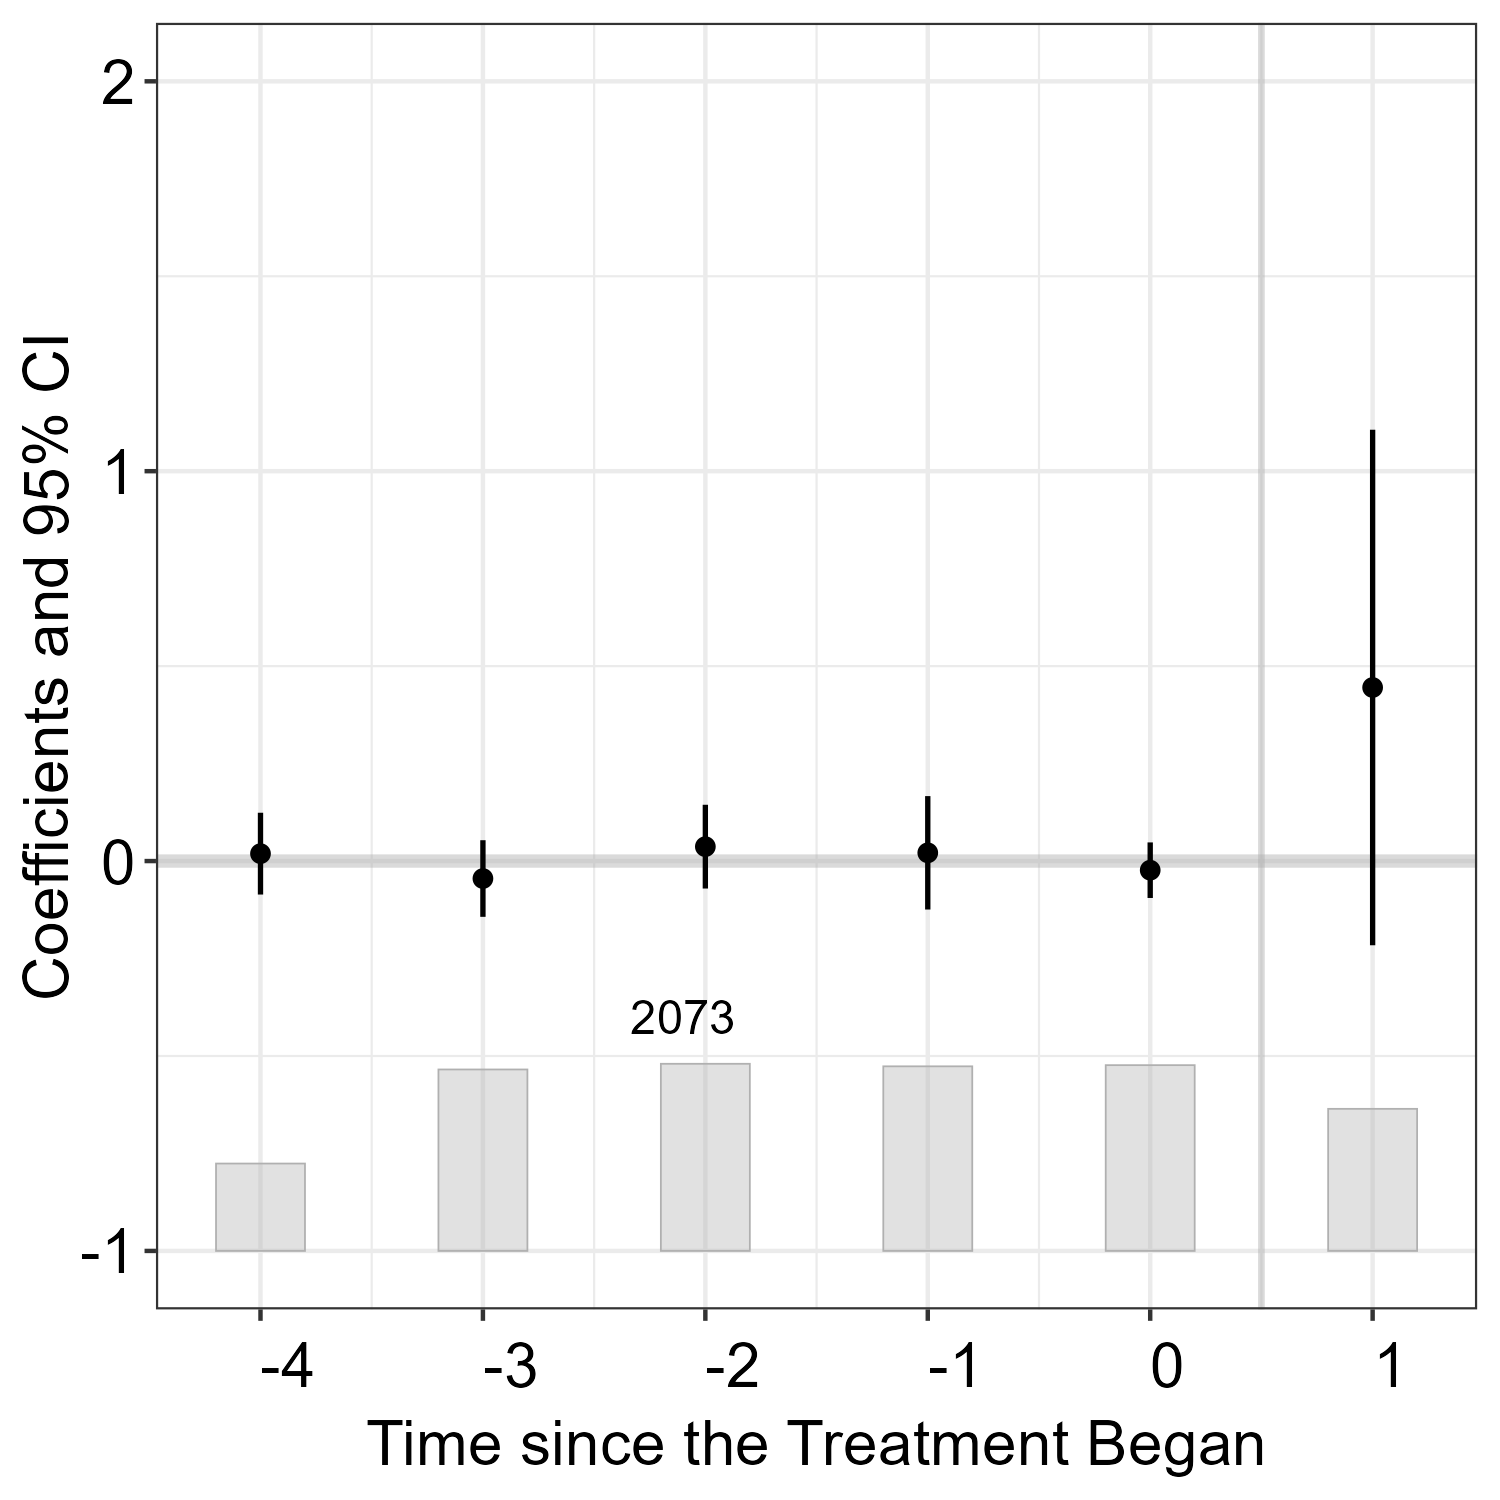
\includegraphics[width = 0.22\textwidth]{figure/fect/kogan_fect_entry.png}  & 
   \hspace{-2em}  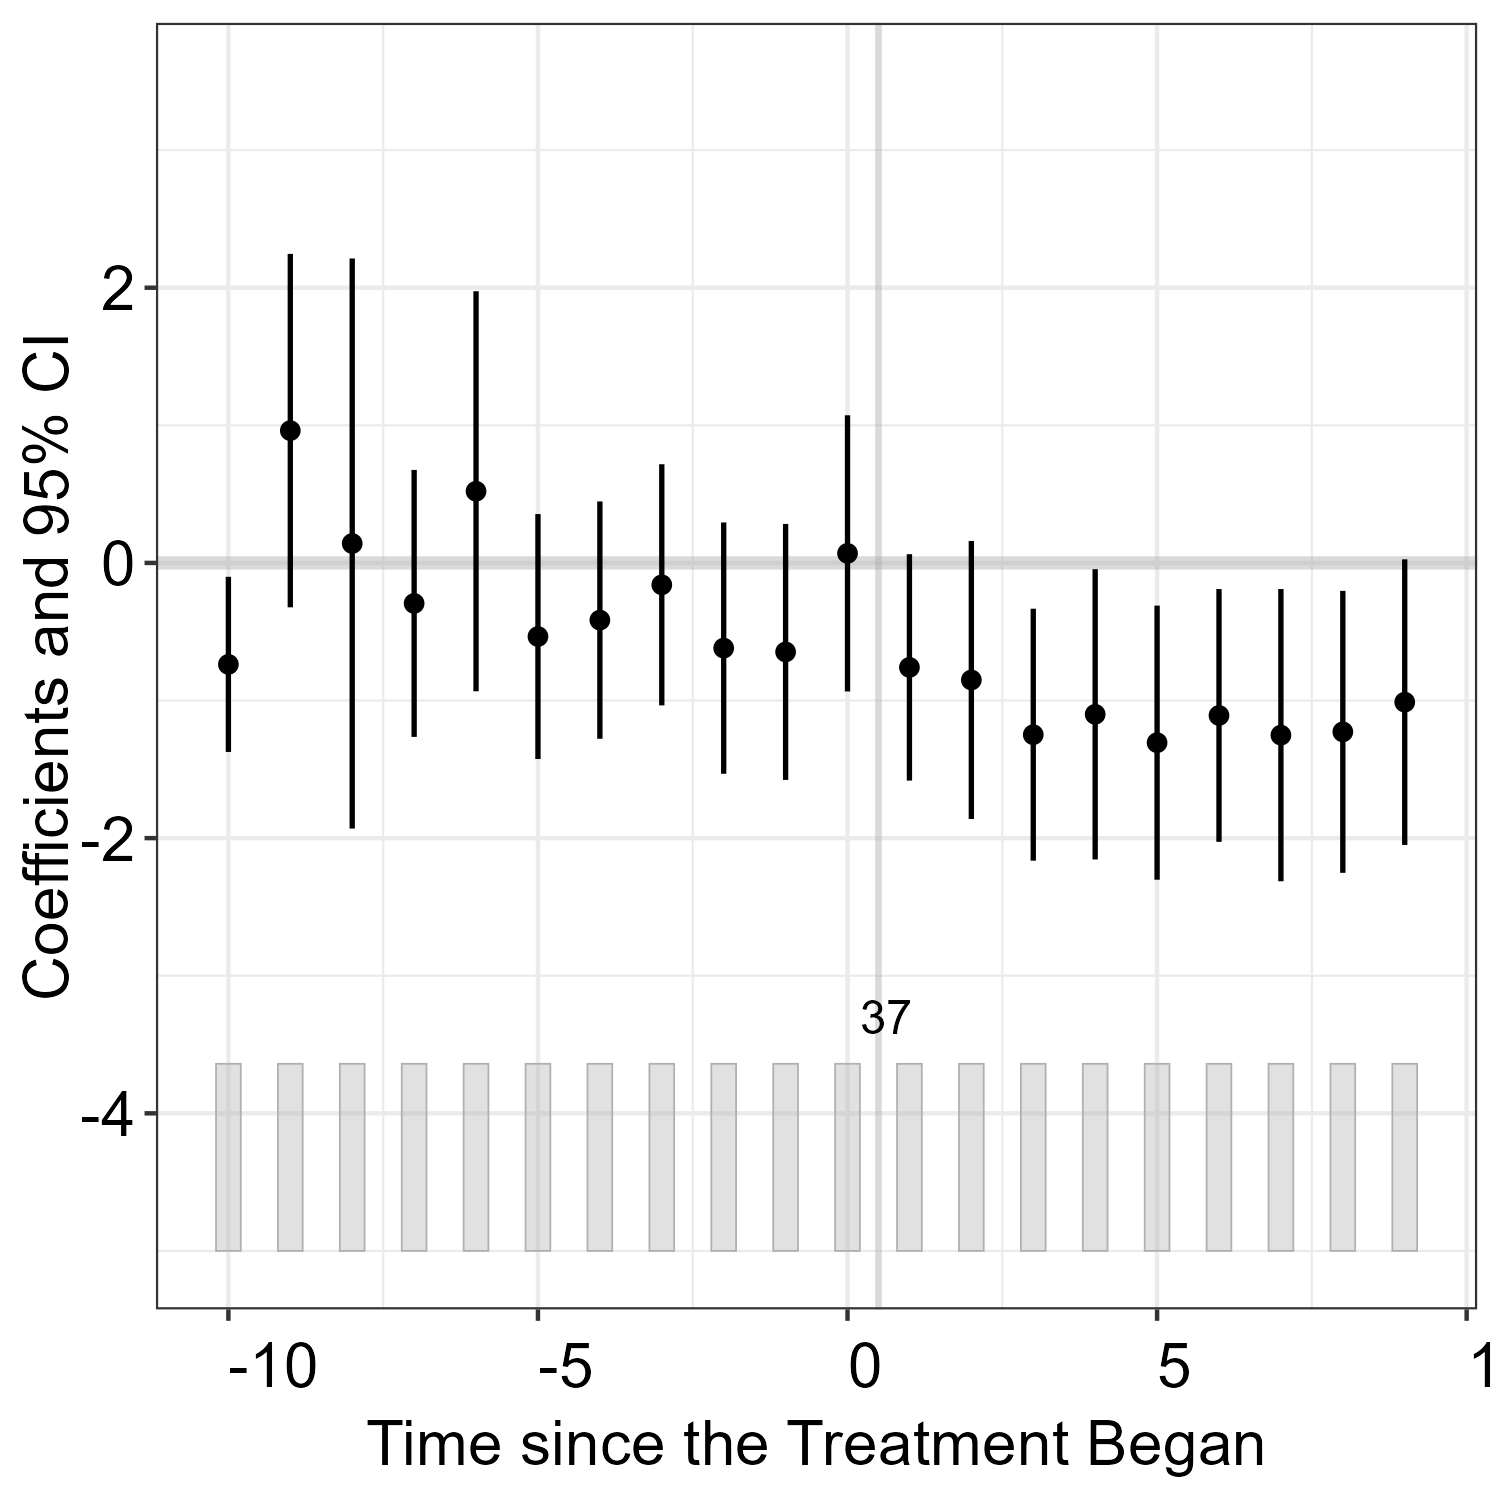
\includegraphics[width = 0.22\textwidth]{figure/fect/magaloni_fect_entry.png} &
   \hspace{-2em}  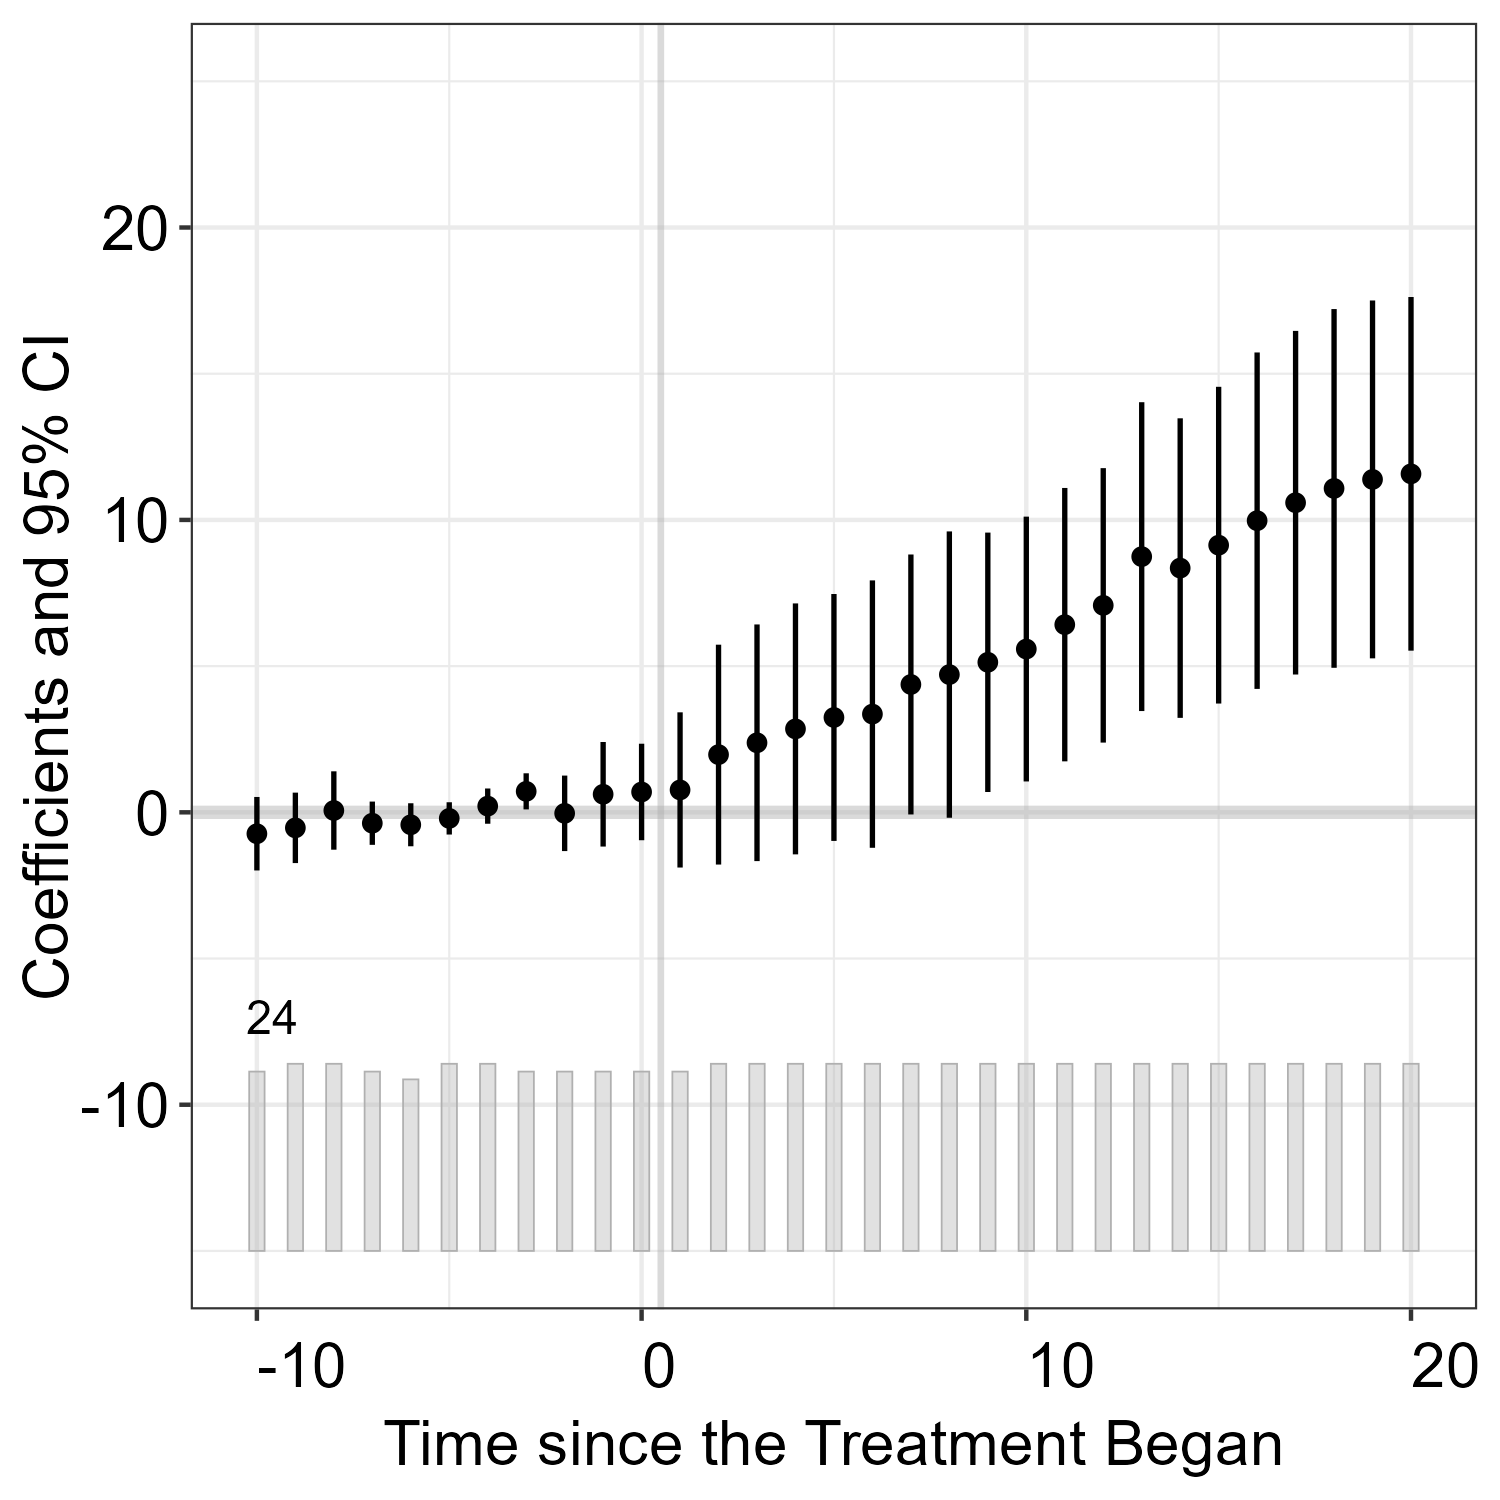
\includegraphics[width = 0.22\textwidth]{figure/fect/paglayan_fect_entry.png} &
      \hspace{-2em} 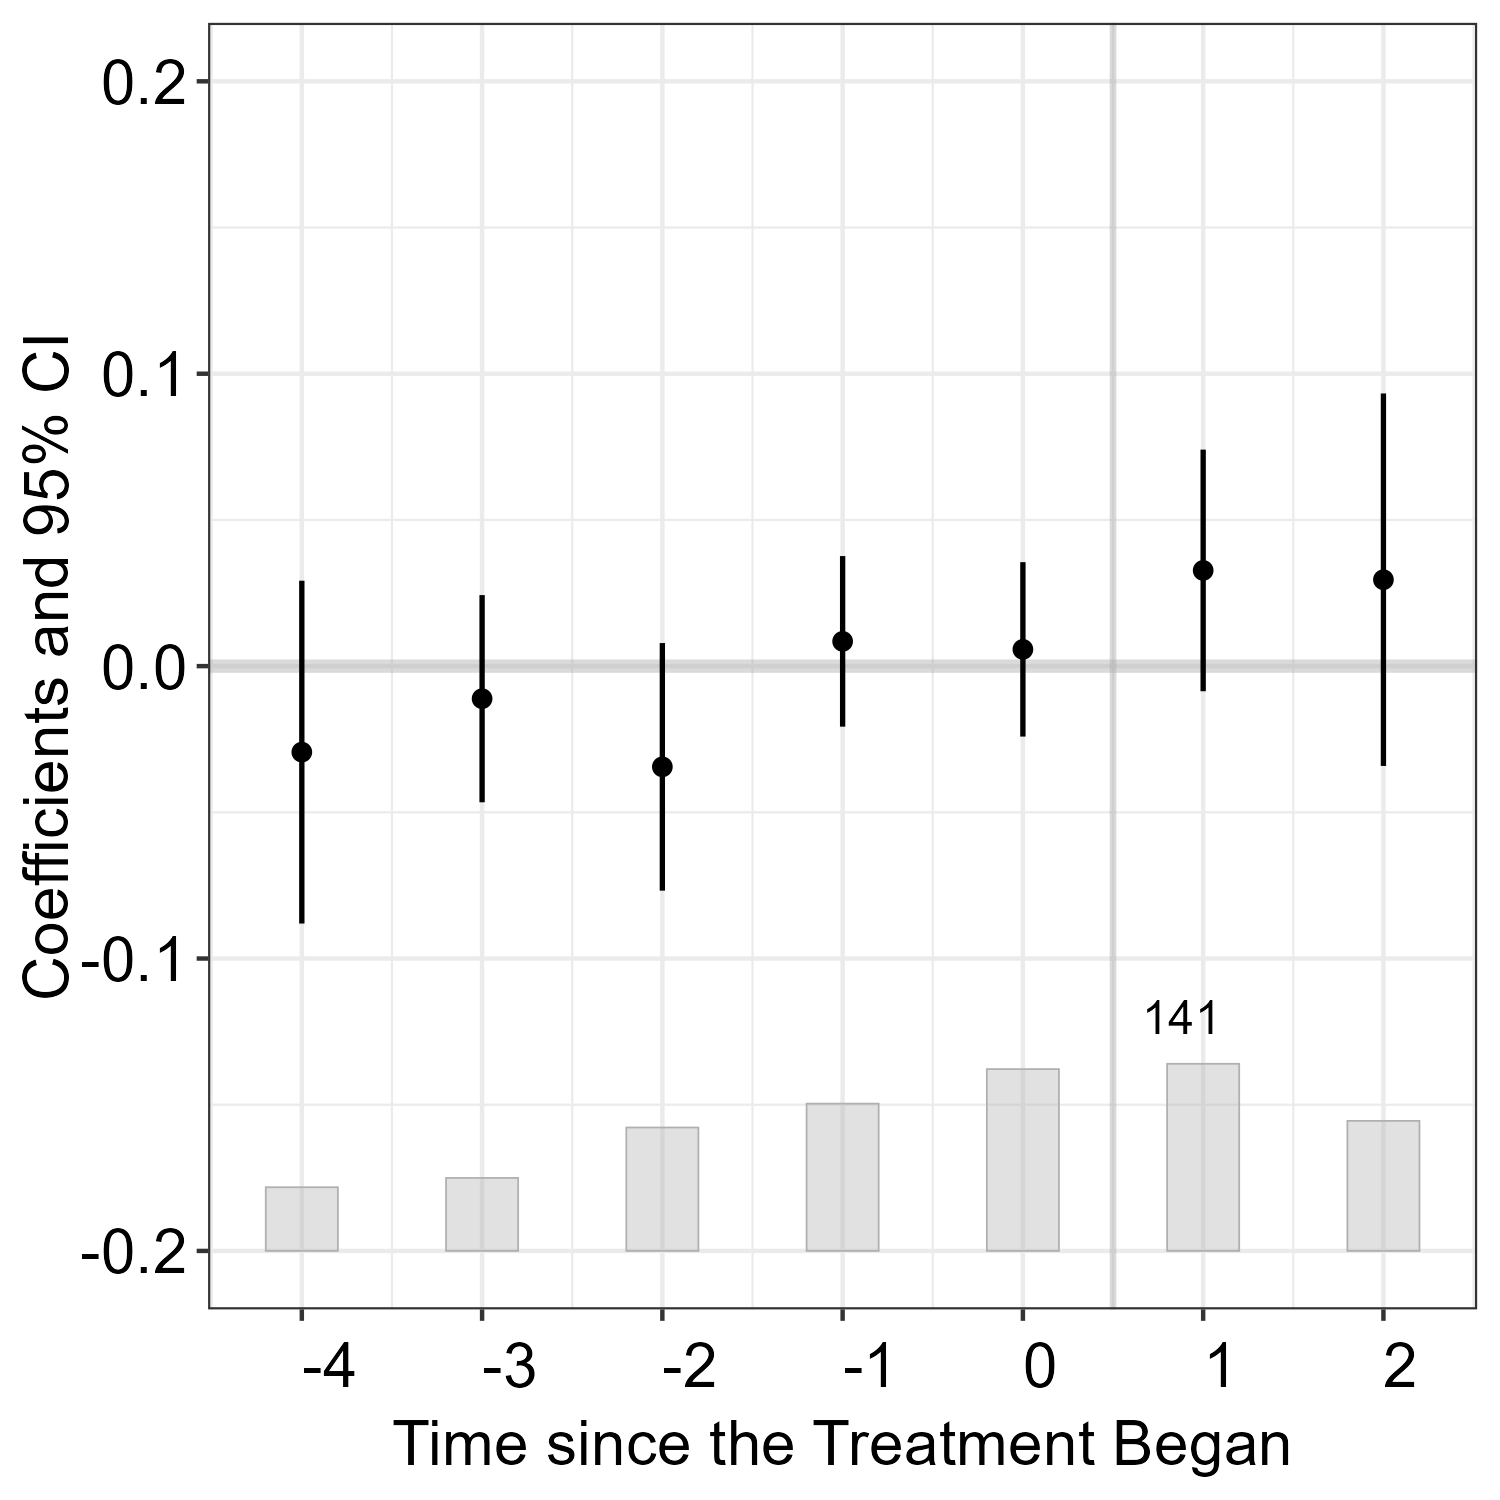
\includegraphics[width = 0.22\textwidth]{figure/fect/paysona_fect_entry.png}\\ \\ 
   \citet{Payson2020jop} \newline  ATT: 13.04 (8.44); \newline $p$-values: 0.92, 0.03 & 
   \citet{Pierskalla2018} \newline ATT: -0.07 (0.04); \newline $p$-values: 0.01, 0.00 &
   \citet{Ravanilla2022} \newline ATT:  0.36 (0.18); \newline $p$-values: n.a., n.a. &
      \citet{Schafer2021} \newline  ATT: -0.02 (0.003) ; \newline $p$-values: 0.02, 0.00\\ 
   \hspace{-2em}  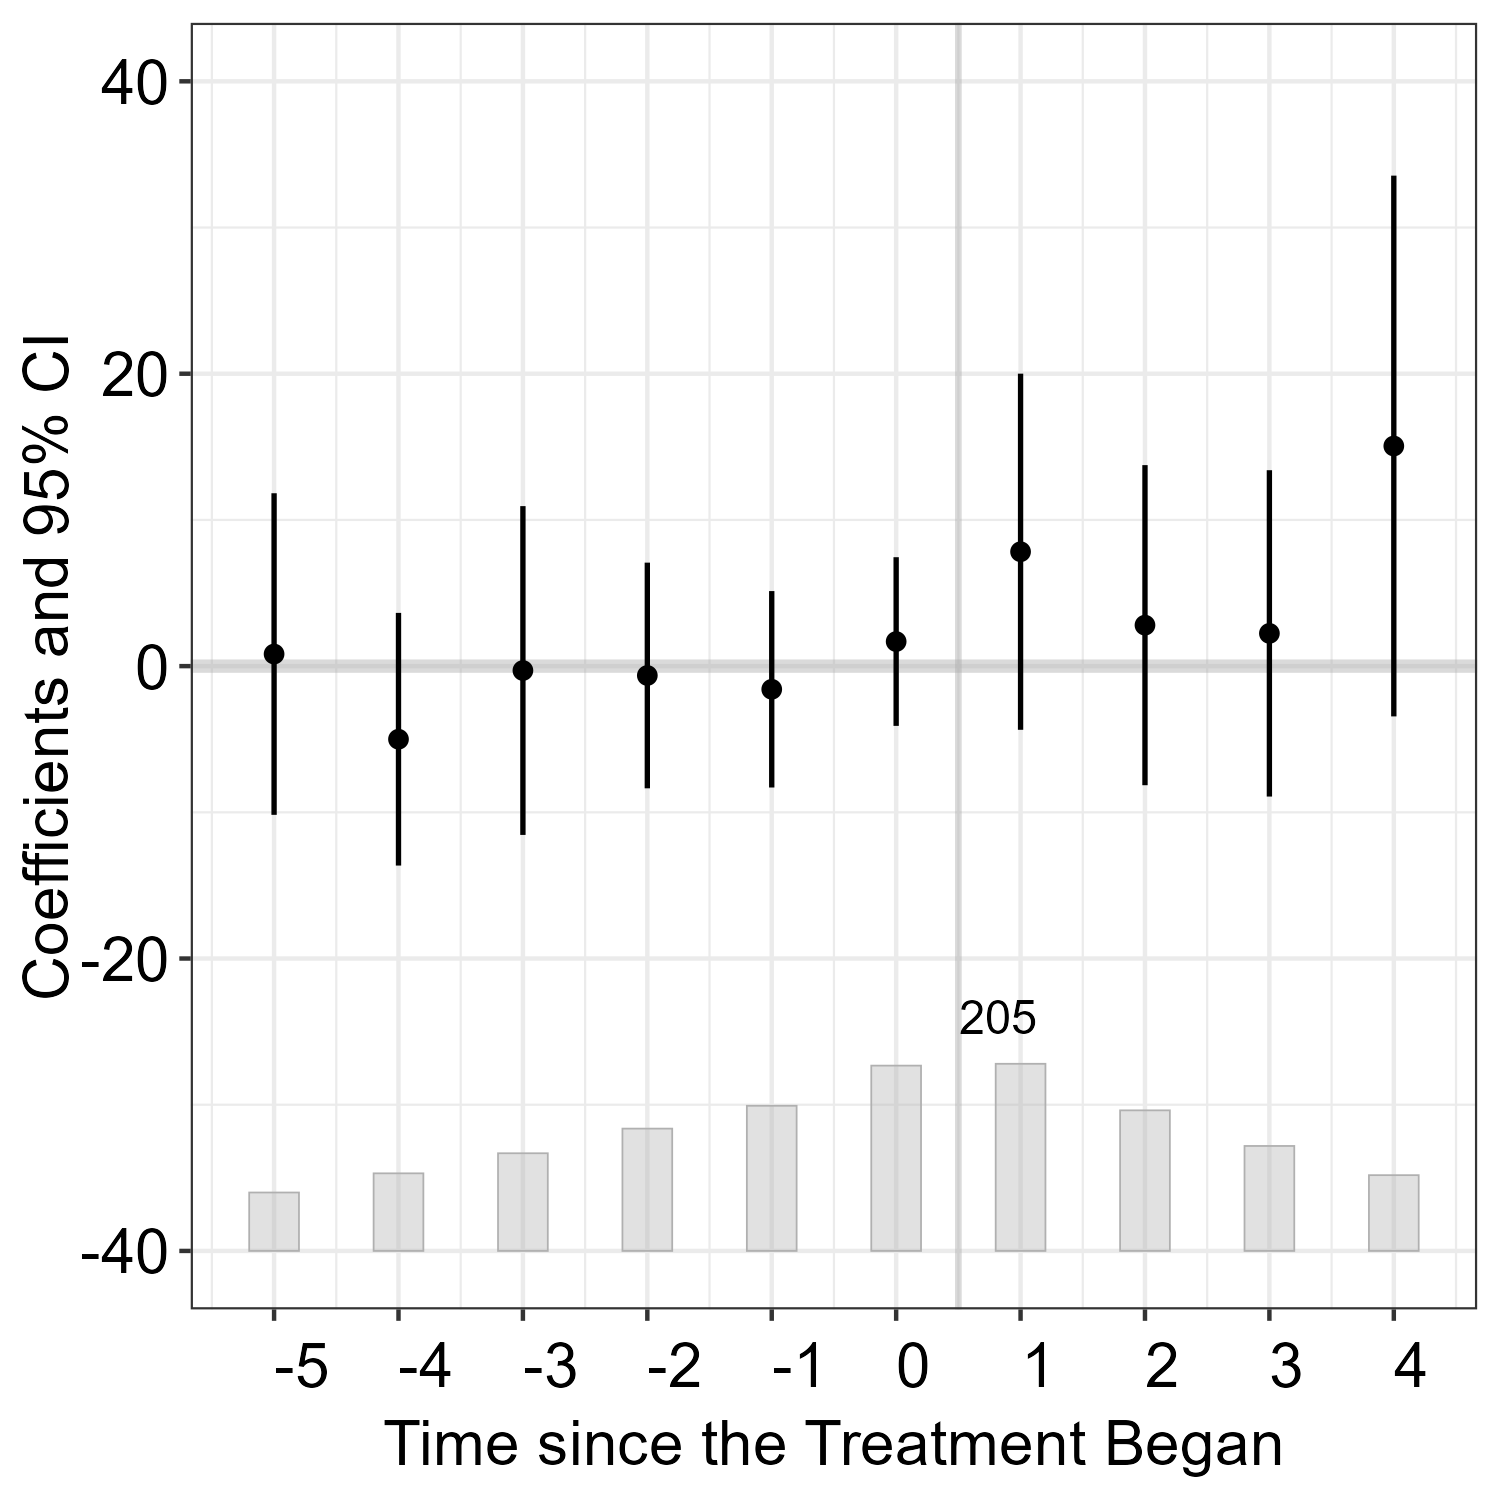
\includegraphics[width = 0.22\textwidth]{figure/fect/paysonb_fect_entry.png} & 
   \hspace{-2em}  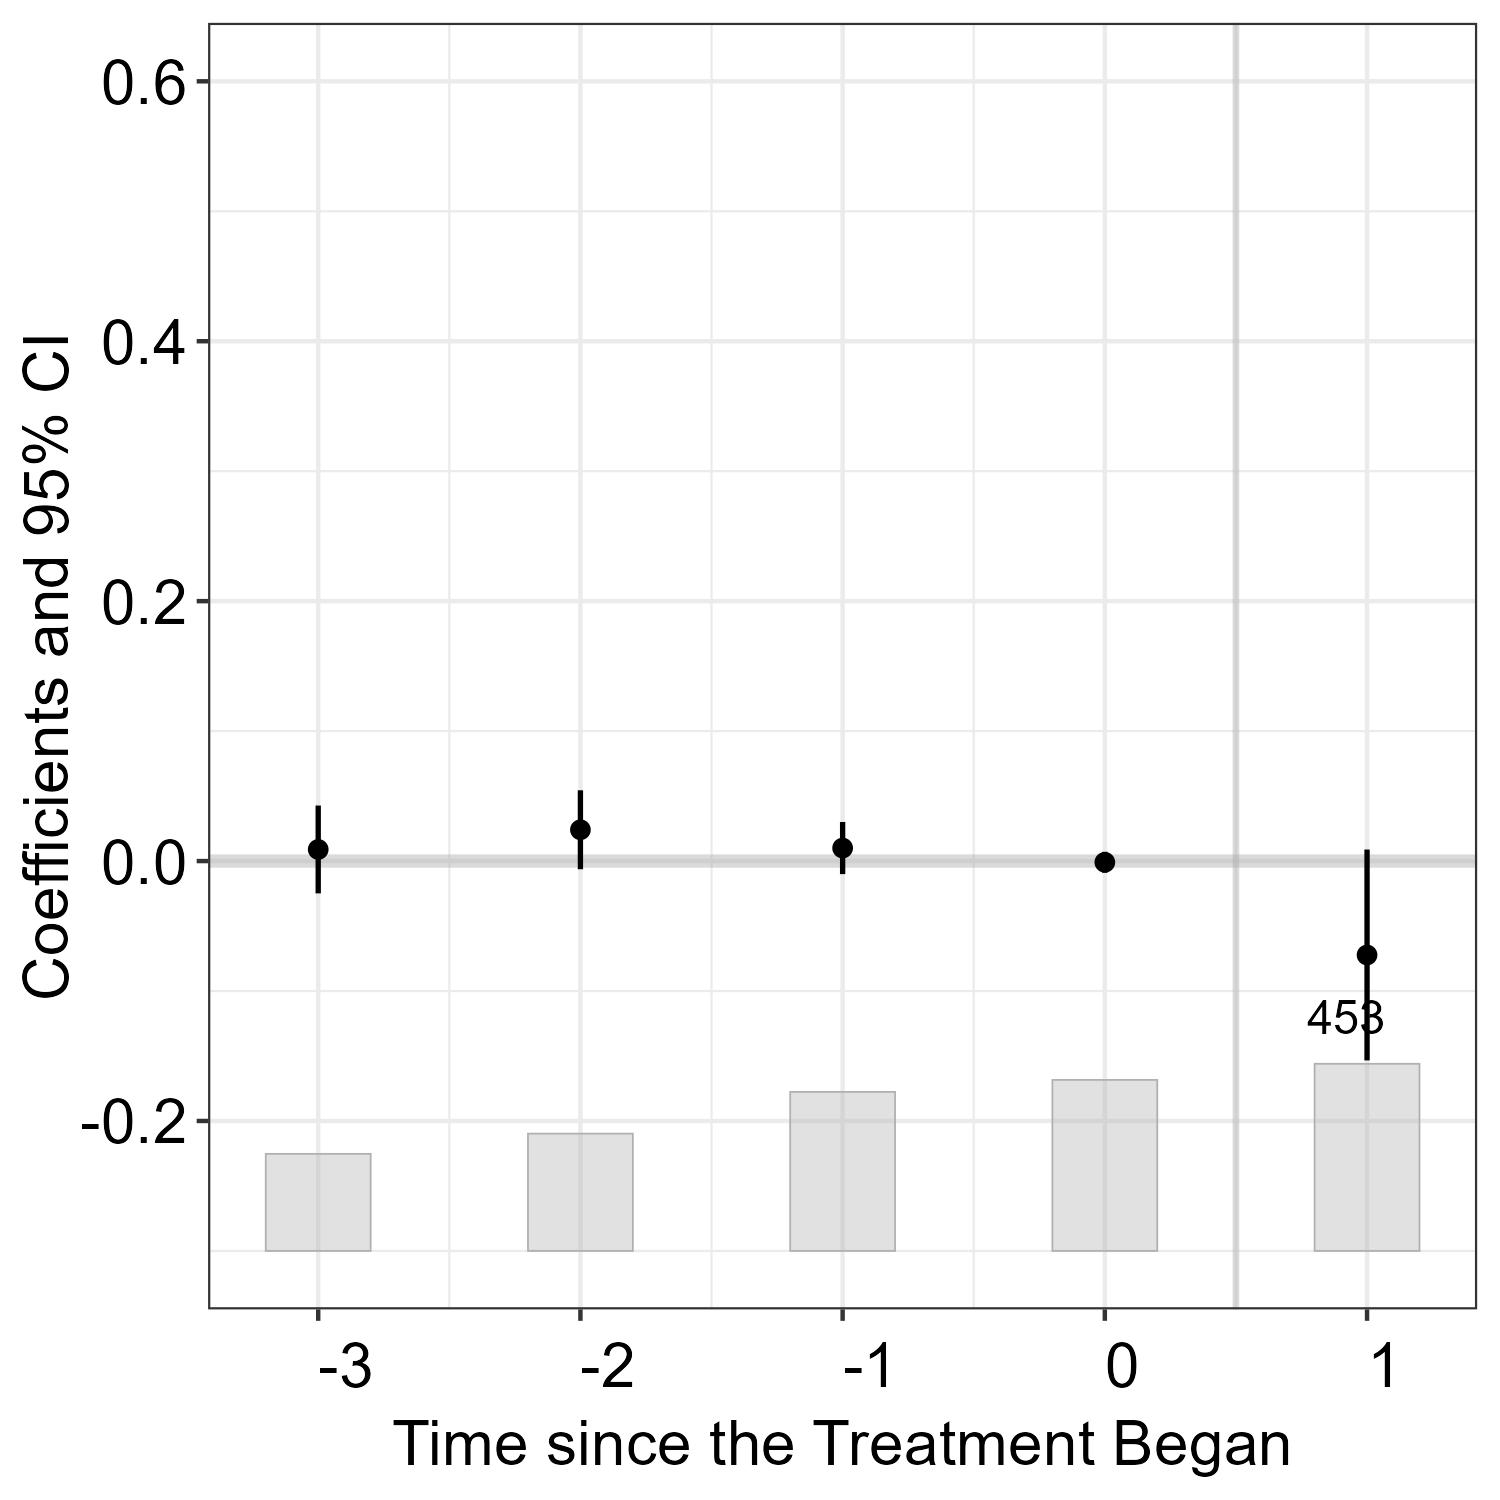
\includegraphics[width = 0.22\textwidth]{figure/fect/Pierskalla_fect_entry.png} &
   \hspace{-2em}  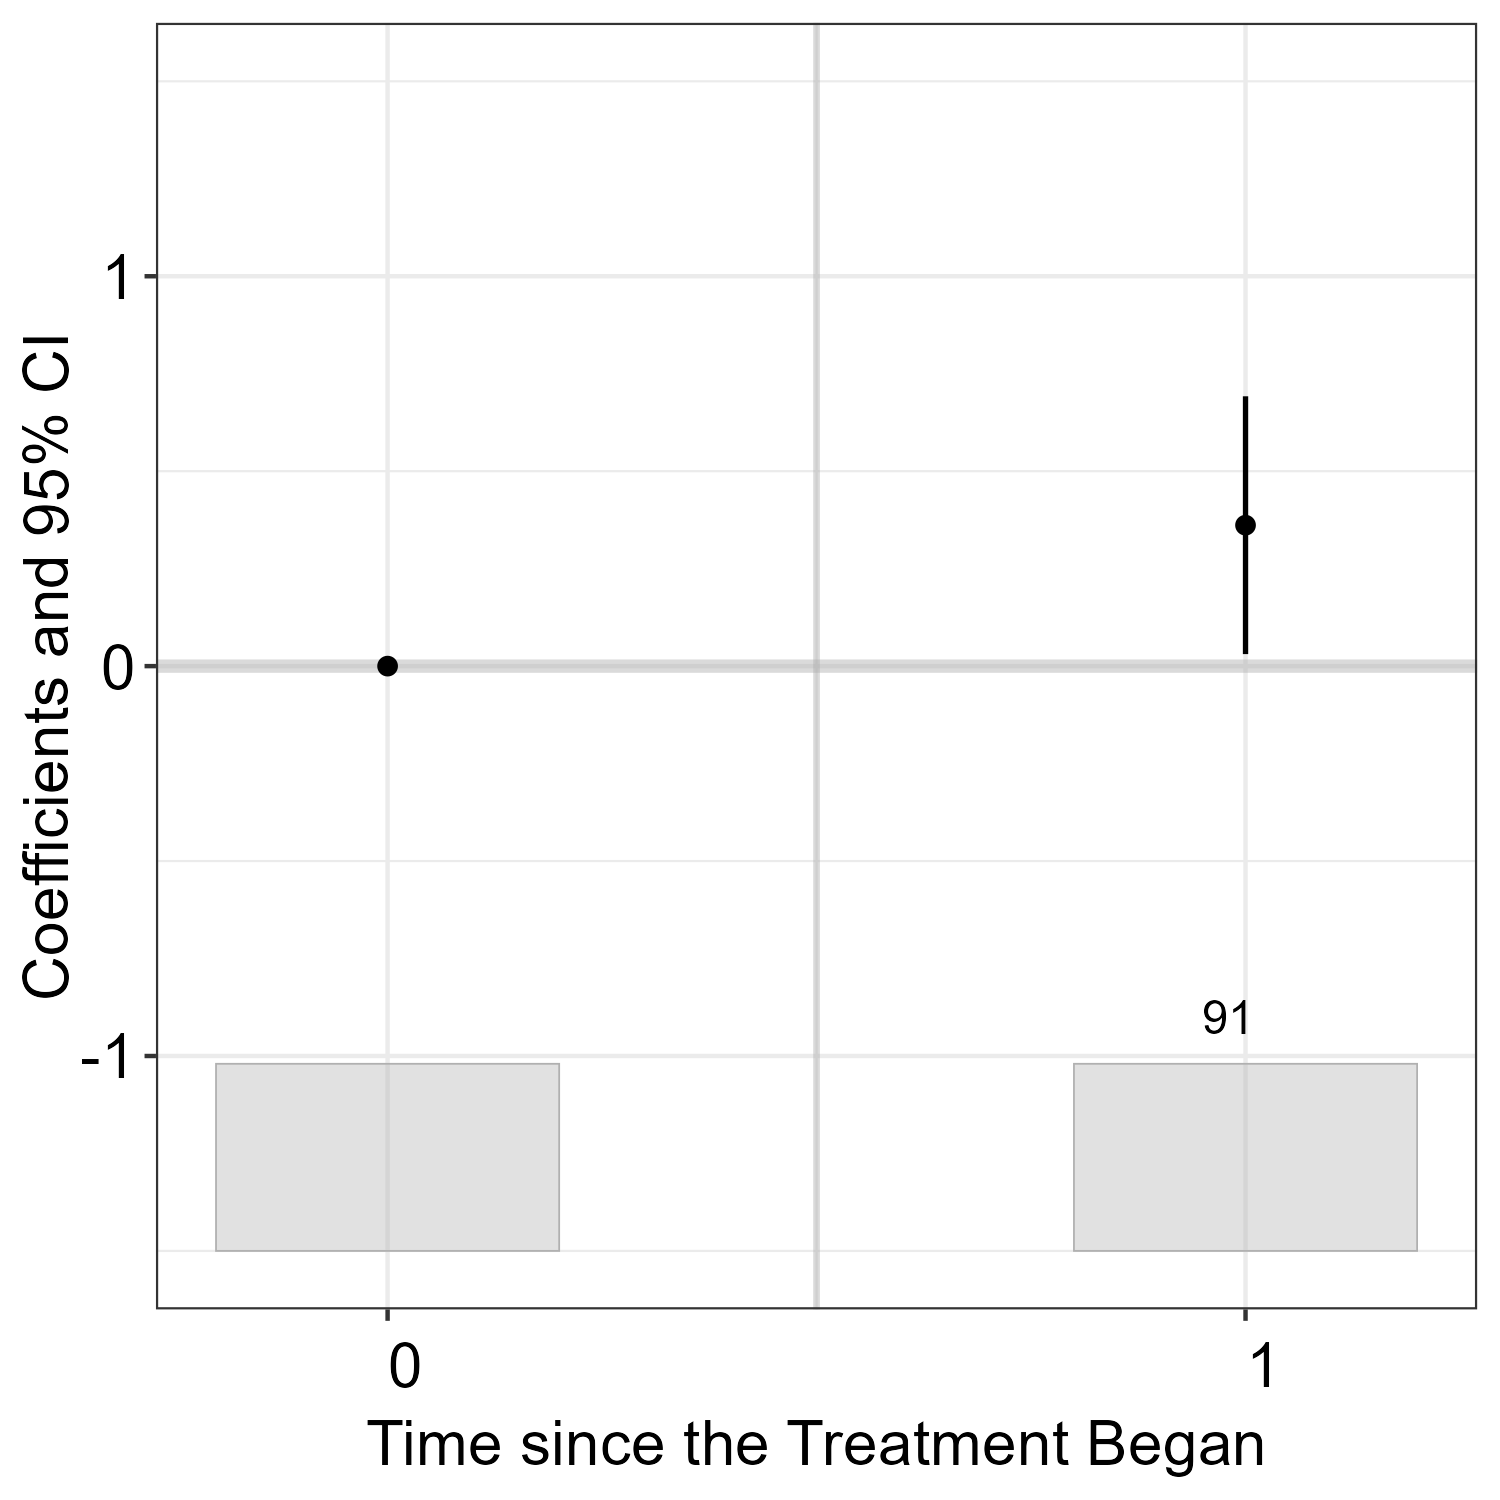
\includegraphics[width = 0.22\textwidth]{figure/fect/ravanilla_fect_entry.png} & 
      \hspace{-2em}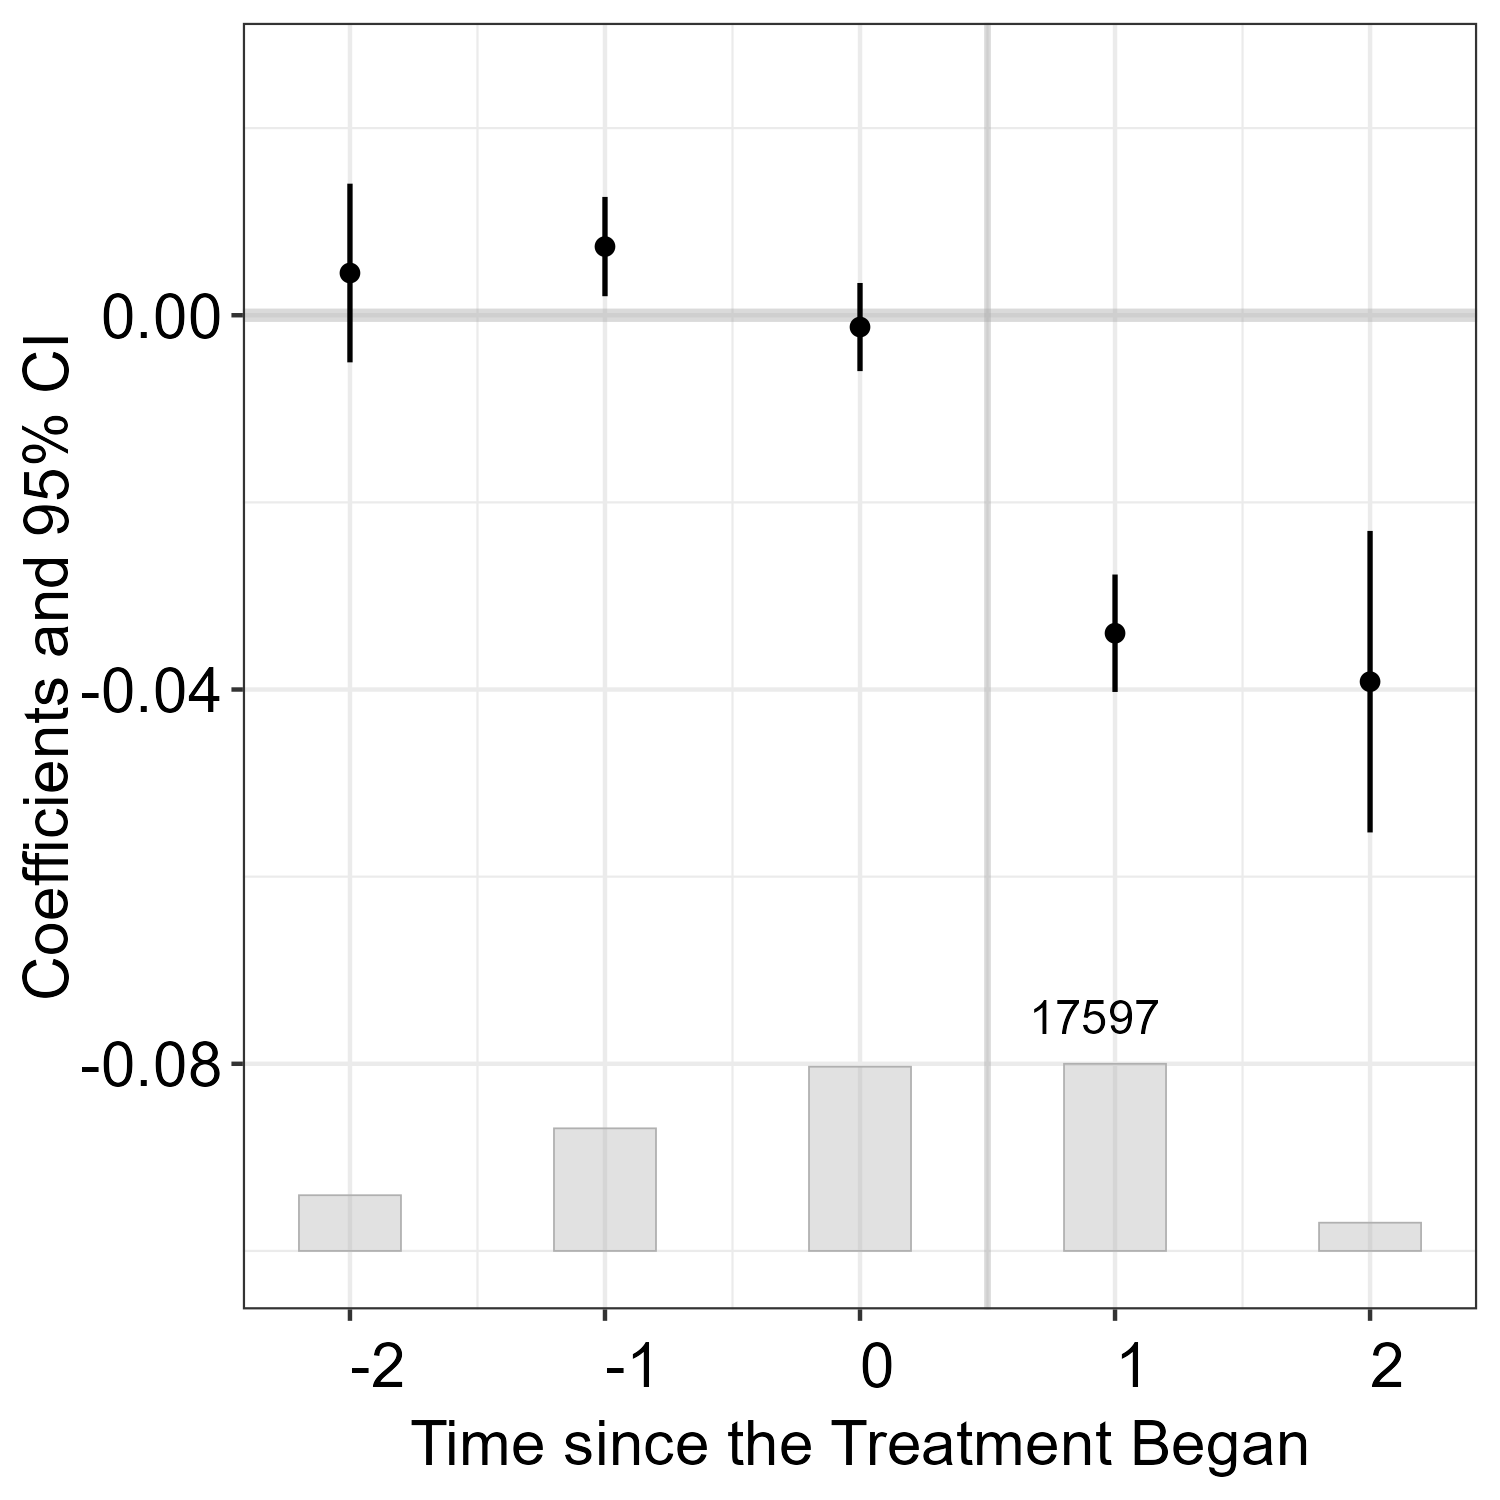
\includegraphics[width = 0.22\textwidth]{figure/fect/schafer_fect_entry.png} \\ \\ 
   \citet{Schubiger2021} \newline ATT: 0.05 (0.01); \newline $p$-values: n.a., n.a.  & 
   \citet{Schuit2017} \newline  ATT:  -0.16 (0.04) ; \newline $p$-values:  0.94, 0.02 &
   \citet{Trounstine2020} \newline ATT: -0.06 (0.01); \newline $p$-values: 0.00, 0.00  &   
   \citet{Weschle2021} \newline ATT: 1.11 (0.72); \newline $p$-values: 0.00, 0.58\\
   \hspace{-2em}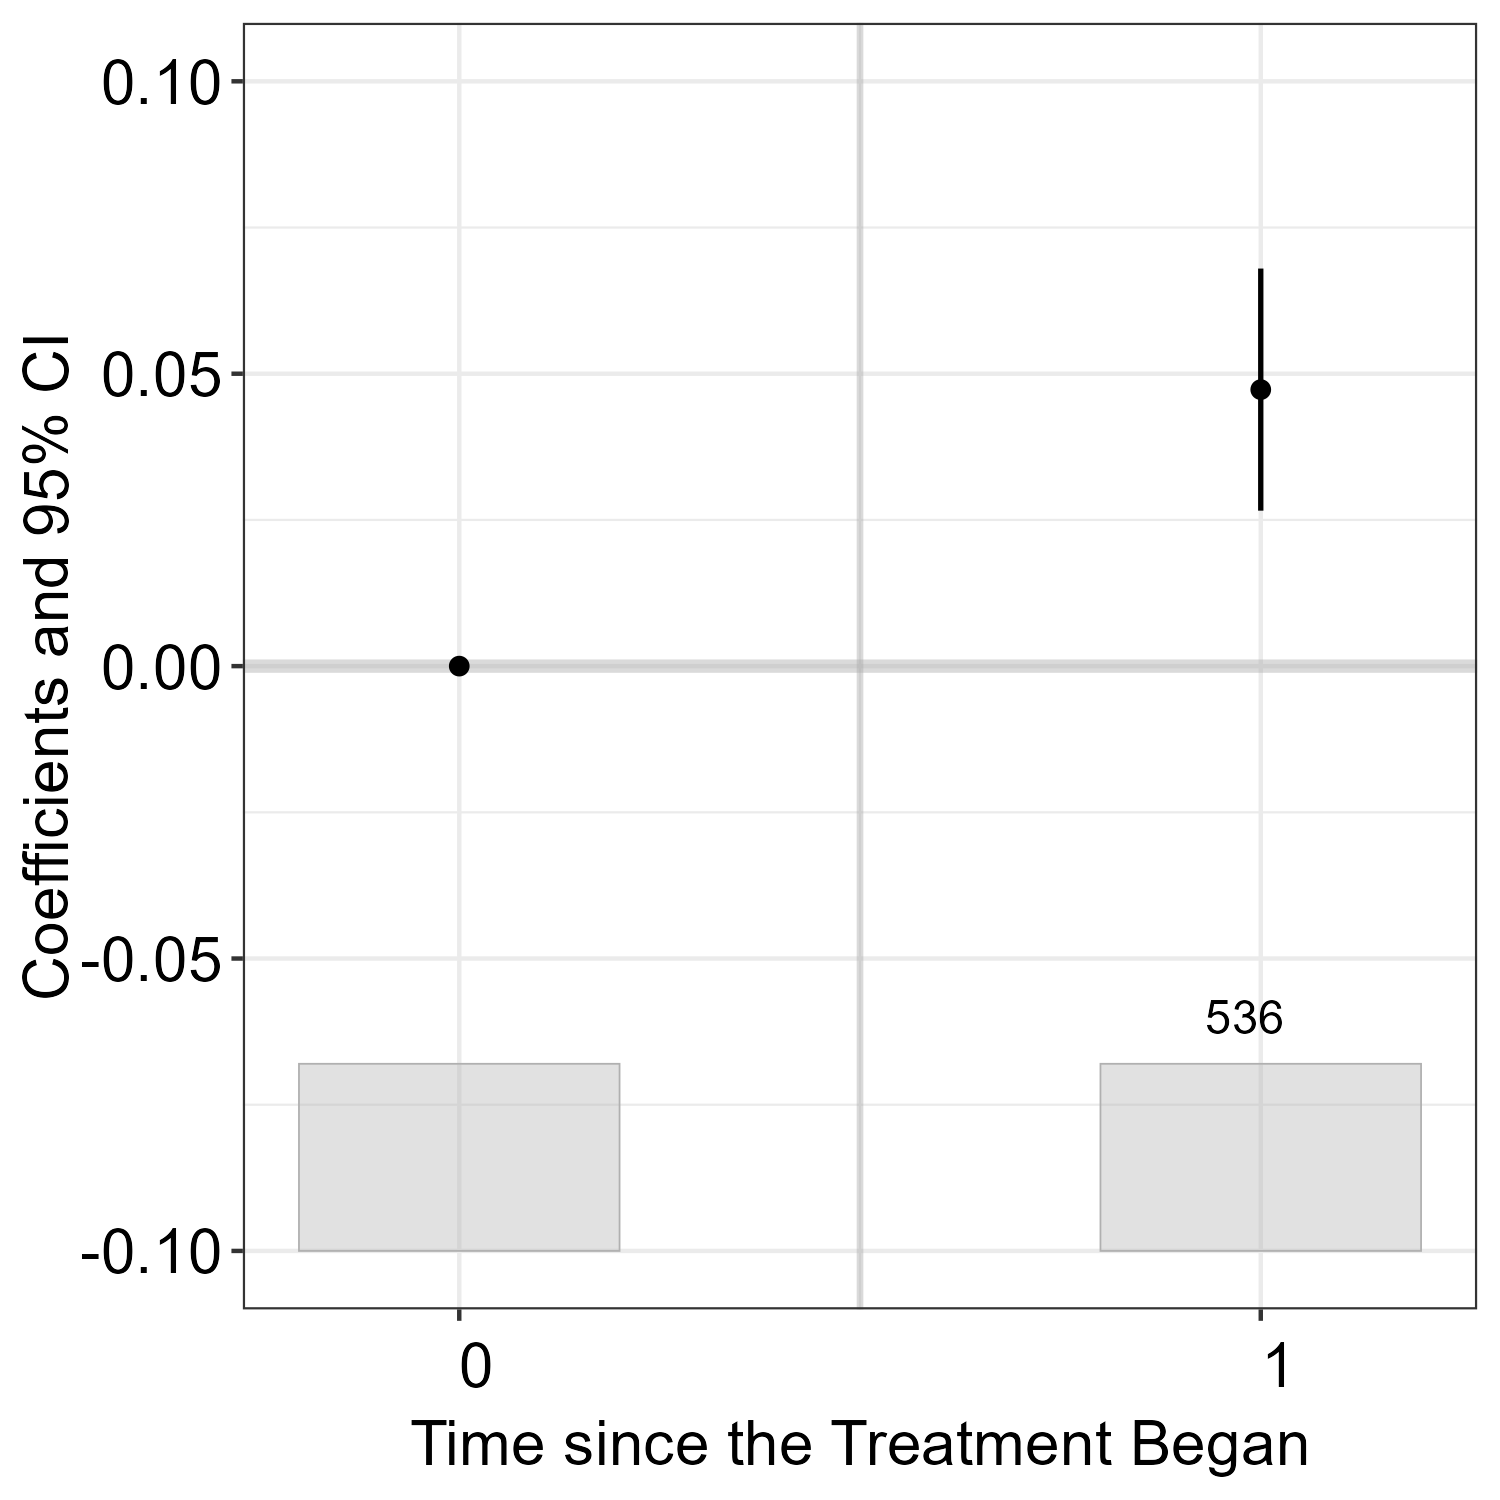
\includegraphics[width = 0.22\textwidth]{figure/fect/Schubiger_fect_entry.png} &
   \hspace{-2em}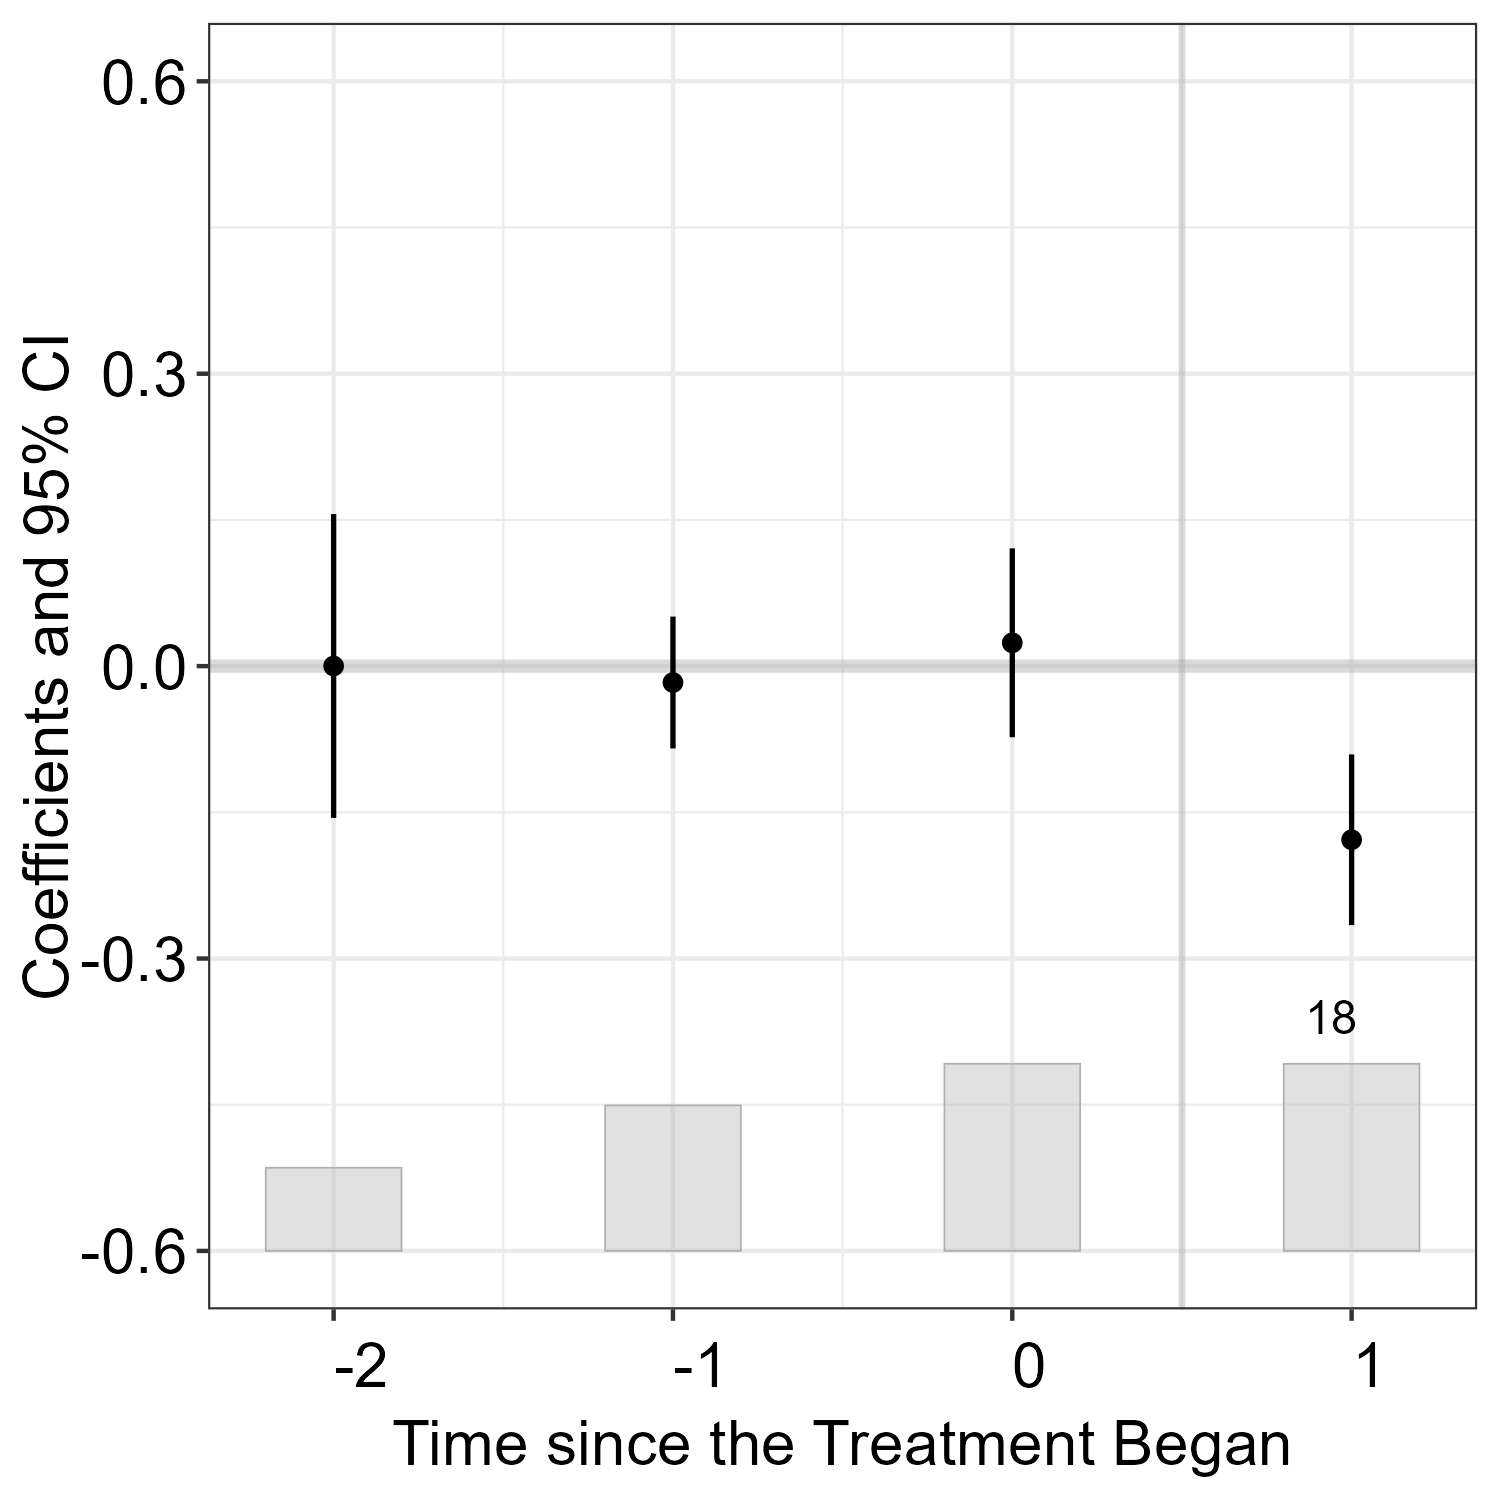
\includegraphics[width = 0.22\textwidth]{figure/fect/Schuit_fect_entry.png} &
   \hspace{-2em} 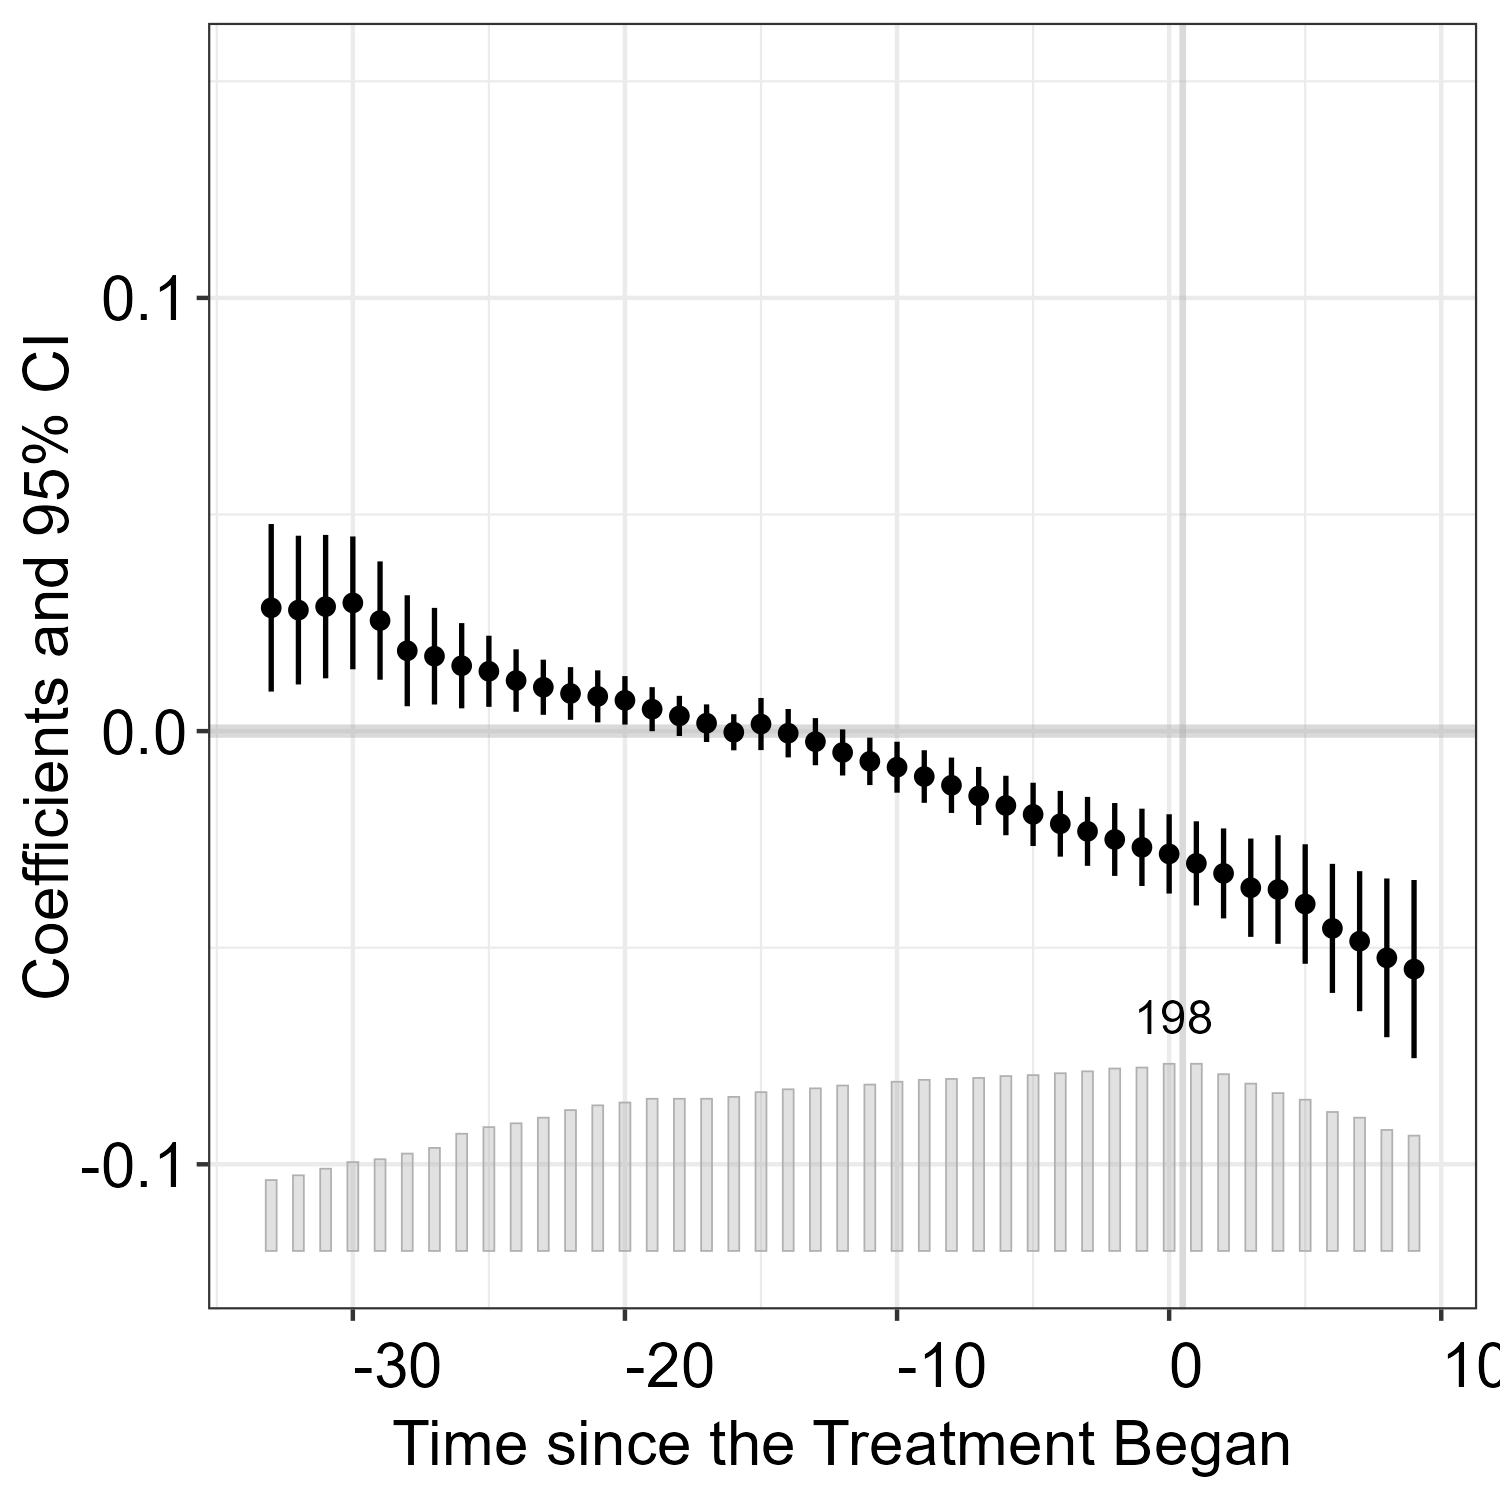
\includegraphics[width = 0.22\textwidth]{figure/fect/trounstine_fect_entry.png} &
      \hspace{-2em} 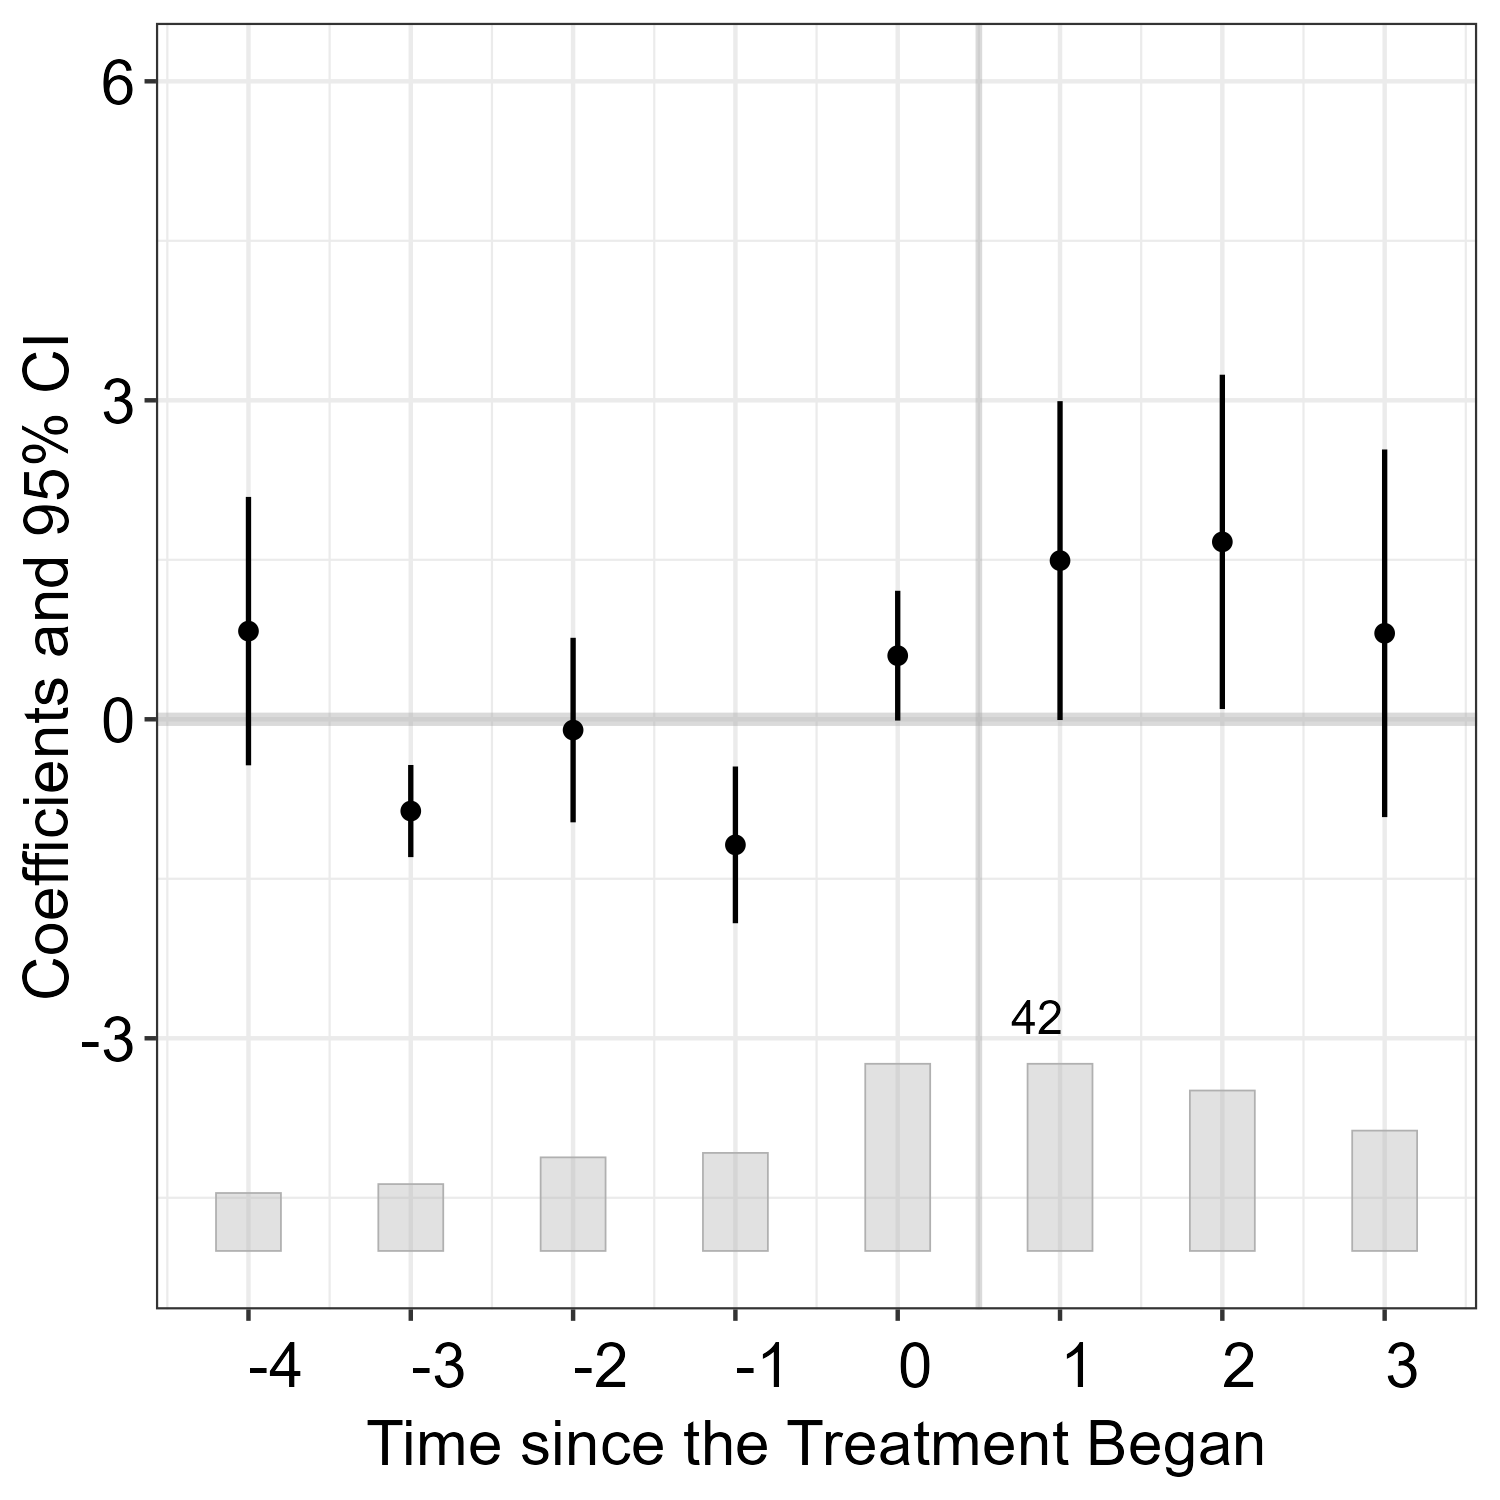
\includegraphics[width = 0.22\textwidth]{figure/fect/weschle_fect_entry.png}\\ \\
   \citet{Zhang2021jop} \newline ATT: 0.11 (0.06); \newline $p$-values: n.a., n.a.  \\
   \hspace{-2em} 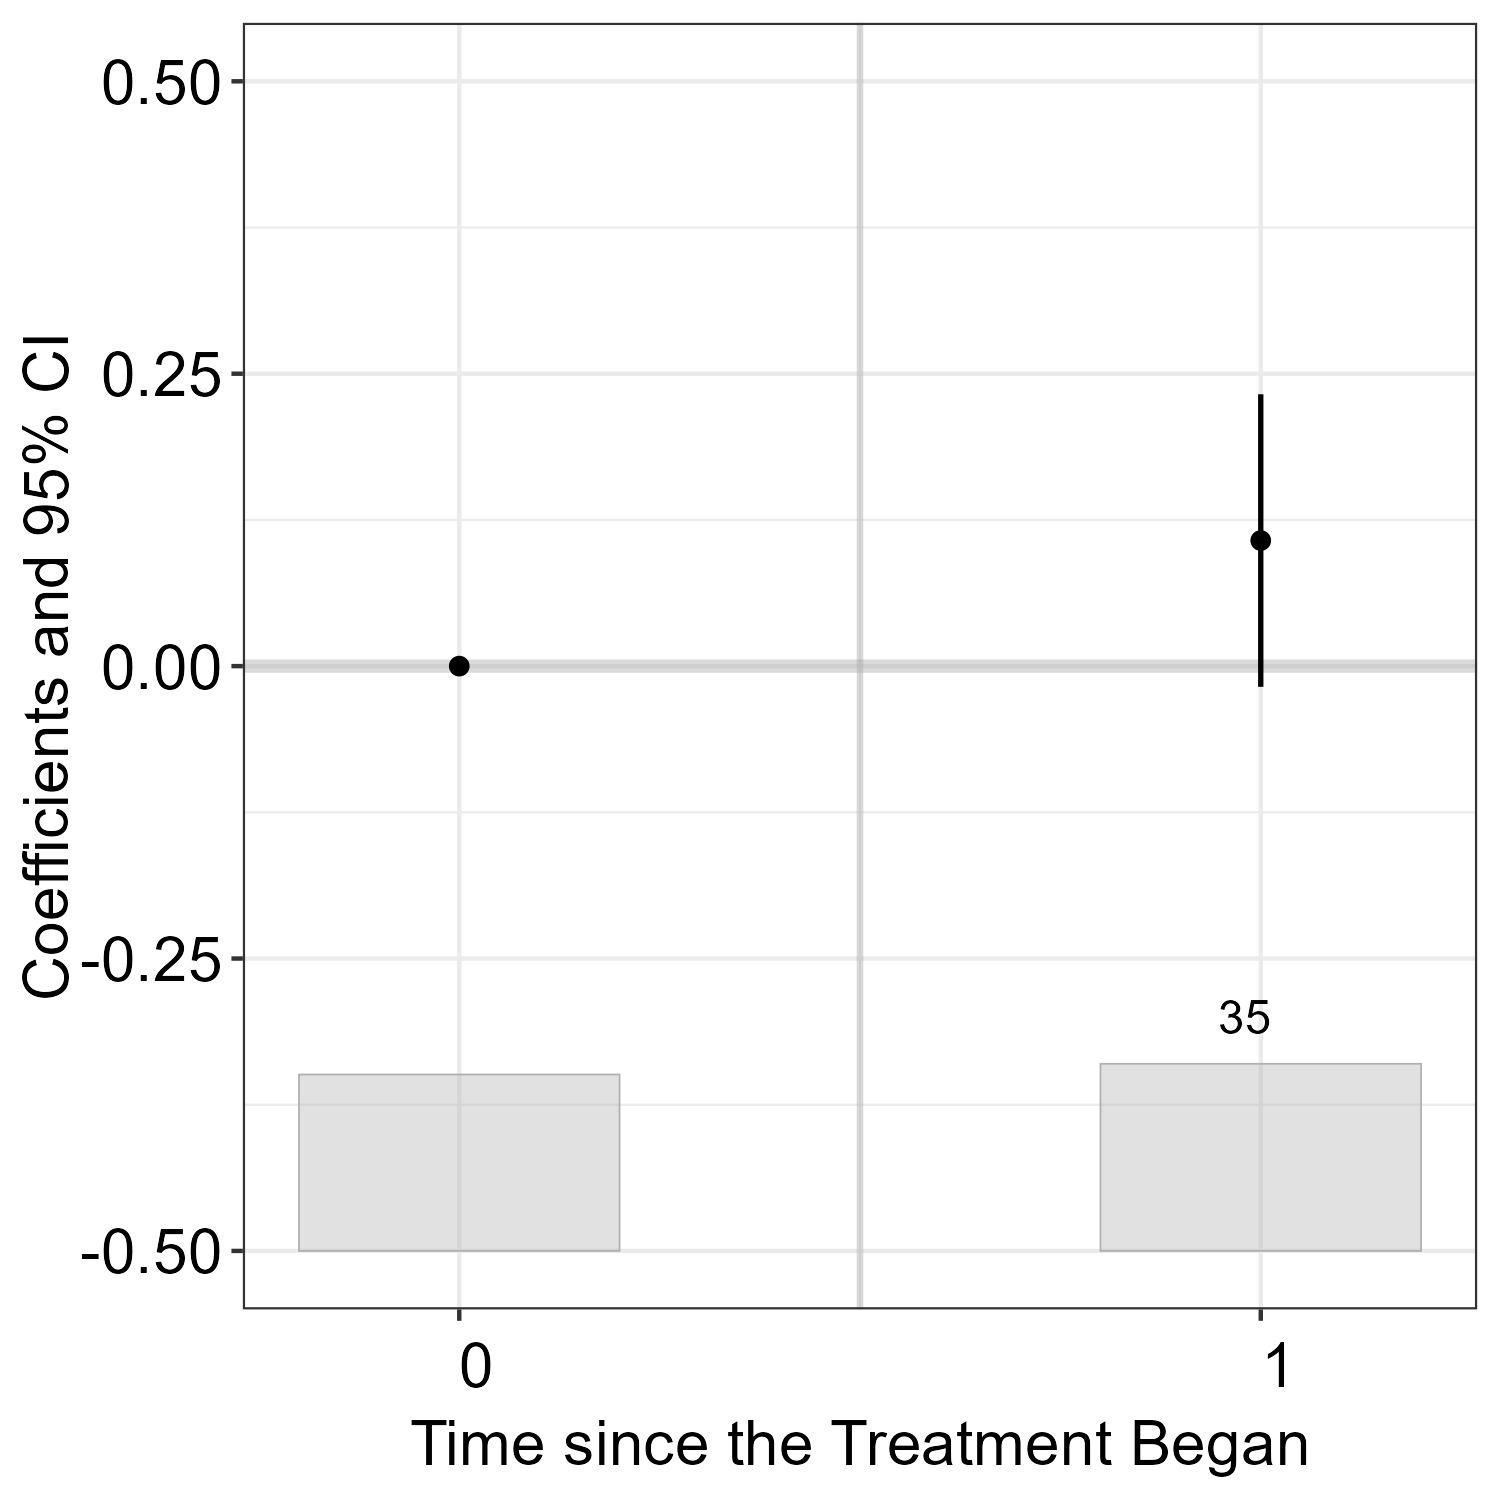
\includegraphics[width = 0.22\textwidth]{figure/fect/zhang_fect_entry.png} &
   \multicolumn{3}{L{11.8cm}}{\scriptsize\textbf{Note:} We report the estimated ATT and corresponding bootstrap SEs (in parentheses) using \texttt{FEct}. We also provide the $p$-values from the $F$ test and equivalence test. Rejecting the null in the $F$ test indicates potential violations of the PTA while rejecting the null in the equivalence test provides evidence in support of the PTA. These tests are infeasible for four cases with only one pretreatment period.} \\ 
\end{tabular}}}
\end{minipage}\vspace{-0.5em}
\end{figure}

\paragraph*{Allowing mild PTA violations causes most results to lose power.} Although the recent methodological literature heavily focuses on HTE, PTA violations remain a primary concern in practice, despite having been a well-known pitfall for some time now. Notably, over half of the studies in our sample do not include an event-study plot of any kind in the main text or appendices. In Figure~\ref{fg:dynamic}, we present the event-study plot based on estimates from \texttt{FEct} for all papers in our sample. We also report the ATT estimates and their bootstrapped SEs, as well as the $p$-values of the $F$ tests and equivalence tests used to assess pretrends. Due to space limitations, we present the event-study plots from other estimators, as well as results from the placebo tests, robust CSs, and sensitivity analyses, in the SM. 


The encouraging news is that in over 40\% of the studies, we have fairly substantial evidence to attest that either the PTA is plausible or its violation is mild. In these instances, the DTE estimates in the pretreatment periods hover around zero, and formal statistical tests suggest that the remaining imbalance likely results from randomness in data (i.e., the $F$ test does not reject, and the equivalence test does reject using the $|\wh{ATT}|$ as the equivalence threshold, both at the 5\% level). However, for the majority of the remaining studies, except for a few cases where the PTA is highly implausible, the results are less conclusive. We either lack the statistical power or a sufficient number of pre-treatment periods to reliably assess the plausibility of the PTA.


\FloatBarrier
% Honest CI


What is much more concerning is that when potential PTA violations are considered, even very mild ones benchmarked against estimated pretrends, most studies lose statistical power. As previously noted, 11 studies lost statistical significance at the 5\% level once we apply the imputation estimator. Relaxing the PTA poses an even greater threat. Figure~\ref{fg:power}(a) shows that the null of no effect is rejected at the 5\% level in only in a small minority of the studies---seven among 31 studies (23\%) for which such an analysis is feasible---when using the partial identification procedure recommended by \citet{rambachan2023more} with $\bar{M} = 0.5$. 
\begin{figure}[!ht]
  \caption{Allowing PTA Violations with Robust Confidence Sets}\label{fg:power}
  \centering
  \vspace{-0.5em}
  \begin{minipage}{1\linewidth}{
  \begin{center}  
  \subfigure[Robust infernece under PTA violations]{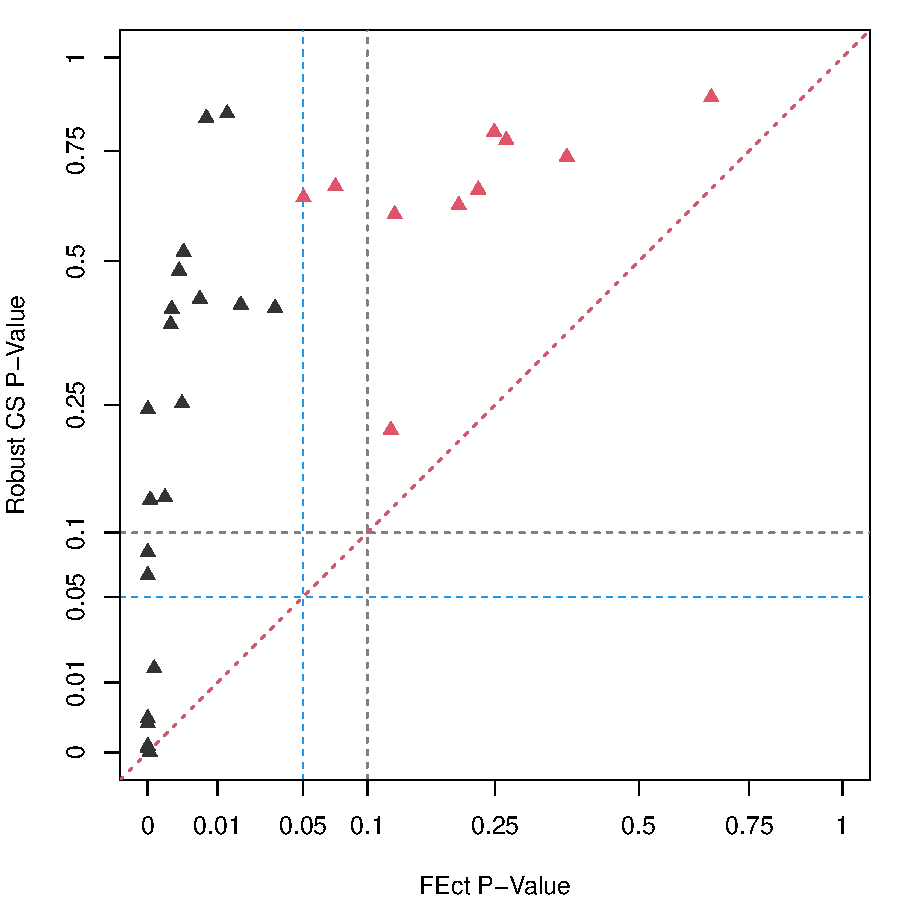
\includegraphics[width = 0.45\textwidth]{figure/summary/honest50p_fect.pdf}}
  \vspace{-1em}
  \hspace{1em}
  \subfigure[Distribution of $\tilde{M}$]{\includegraphics[width = 0.45\textwidth]{figure/summary/Mbar_histp.pdf}}
  \end{center}
  {\footnotesize\textbf{Note:} Subfigure (a) shows the $p$-values of partially identified ATT estimates using \texttt{FEct} under restricted RM PTA violations with $\bar{M} = 0.5$ versus \texttt{FEct} $p$-values assuming the PTA is satisfied ($\bar{M} = 0$). Squared root scales are used to facilitate visualization. The red triangles represent studies that lose statistical significance when \texttt{FEct} is used under the PTA. Subfigure (b) is a histogram of $\tilde{M}$, breakdown values of $\bar{M}$ for the 31 studies with more than three pretreatment periods; the pink bar represents 11 studies who ATT estimates are statistically insignificant at the 5\% level using \texttt{FEct}.}}
  \end{minipage}\vspace{-1em}
\end{figure}
Figure~\ref{fg:power}(b) displays the distribution of breakdown values $\tilde{M}$. Among all 31 studies with at least three pretreatment periods, the median is 0.18 and the mean is 0.37. Focusing only on the 20 studies that remain statistically significant at the 5\% level with \texttt{FEct}, the median and mean are as low as 0.33 and 0.58, respectively. Although using HTE-robust estimators with robust CSs does not necessarily ``overturn'' results in most of the paper we reanalyzed, it is evident that the vast majority of studies lack the power to discern the ATT from zero under very mild violations of the key identifying assumption of realistic magnitudes informed by pretrends.


\FloatBarrier

%  $$$$$$\    $$\     $$\                           
% $$  __$$\   $$ |    $$ |                          
% $$ /  $$ |$$$$$$\   $$$$$$$\   $$$$$$\   $$$$$$\  
% $$ |  $$ |\_$$  _|  $$  __$$\ $$  __$$\ $$  __$$\ 
% $$ |  $$ |  $$ |    $$ |  $$ |$$$$$$$$ |$$ |  \__|
% $$ |  $$ |  $$ |$$\ $$ |  $$ |$$   ____|$$ |      
%  $$$$$$  |  \$$$$  |$$ |  $$ |\$$$$$$$\ $$ |      
%  \______/    \____/ \__|  \__| \_______|\__|      
                                                  

\paragraph*{Other issues.} Our reanalysis highlights several additional issues. First, the presence of missing values is widespread. Although most methodological work presumes balanced panels without missing data, in reality, many empirical studies encounter varying degrees of data missingness. We plot patterns of treatment status for each study in the SM. Based on these plots, we see that in some studies the pattern of missingness is either nonrandom or extremely prevalent, which calls into question the reliability and validity of the respective empirical findings. 

Second, we perform carryover effect tests for all studies that feature treatment reversals. If this test fails, it suggests that the treatment effects persist beyond the treatment periods. Among 22 articles, five reject the null hypothesis of no carryover effects at 5\%. Part of the concern is that imputation methods and DID extensions will use control observations from previously treated units to fit the potential outcome model or as comparisons for treated observations, and if there are carryover effects, then the comparisons will become tainted.
LWX \citeyearpar{LWX2022} note that the presence of carryover effects for a limited number of periods is less concerning, as researchers can recode treatment to persist for some time after a unit transitions out of treatment. %By adopting this guideline,
We observe that carryover effects do not substantially alter the findings in most studies. Specifically, when removing two post-treatment periods for studies that reject the null of no carryover effects, the estimates remain similar in magnitude. Additionally, results initially deemed statistically significant continue to maintain their statistical significance (Figure A8 in the SM). Nevertheless, we recommend that researchers make it a practice to check for potential carryover effects, considering the low cost of conducting such tests and adjustments.

Finally, many studies also exhibit sensitivity to model specifications. When we incorporate ULTs into the authors' original specifications, 41\% of studies lose their statistical significance.\footnote{\citet{plumper2019not} raise a cautionary note against the blanket use of fixed effects models in panel data analysis. They show that if both the treatment and the outcome variables are highly autoregressive, these models may lead to spurious correlations.} While the additional parameters reduce efficiency and may lead to biases due to impermissible comparisons \citep{Goodman-Bacon2021-xb}, these results underscore that a significant number of empirical findings in the literature rely heavily on modeling assumptions. Hence, we recommend researchers carefully assess the robustness of their findings using different model specifications in combination with HTE-robust estimators. We reserve a more careful and rigorous analysis of this issue for future studies. 

Relatedly, some studies that we exclude from our sample employ one-way FE or FE at a level different from that at which treatment is assigned. Many of these findings do not hold when we reanalyze them using a TWFE model. We should clarify that this does not imply that the original results are not credible; rather, these models operate under distinct identification assumptions, and there is substantial variation in how much consideration authors give to this point. We notice that some studies do not provide a rationale for their choice to use one-way fixed effects, while others explicitly outline the type of unobserved confounders they intend to control for. In one instance, the authors inaccurately label their specification as a DID design. We emphasize that TWFE and DID are generally not equivalent. This difference becomes even more pronounced when the fixed effects are not assigned at the level of treatment. 




\FloatBarrier

\paragraph*{Summary.} In Table~\ref{tb:summary} below, we summarize the main findings of our reanalysis. The numbers represent the proportion of studies in a given journal or across all journals that fall under the respective category. The first two columns relate to the ratio of the \texttt{FEct} estimator to the TWFE estimator, which proxies the consequences of HTE. Across all journals, this ratio is less than 0.8 in 21\% of studies and less than 0.5 in 5\% of studies, indicating that while HTE might be a significant concern theoretically, its empirical impact may not be as substantial as the existing literature might suggest.
\begin{table}[!ht]
\caption{Summary of Findings}\label{tb:summary}
    \centering\small
    \resizebox{1\textwidth}{!}{
    \begin{tabular}{c|cc|ccc|ccc} \hline\hline
     & \multicolumn{2}{c|}{ Consequence of HTE}  & \multicolumn{3}{c|}{Potential PTA violations}  & \multicolumn{3}{c}{Insufficient power} \\ \hline
 & (1) & (2) & (3) & (4) & (5) & (6) & (7)  & (8) \\ 
 & \texttt{FEct}-TWFE & \texttt{FEct}-TWFE & $F$ test    & Placebo test & Equiv. test        & TWFE \emph{not} & \texttt{FEct} \emph{not} & \texttt{FEct} \emph{not} reject  \\
  Journal &
    Ratio $< 0.8$ & Ratio $< 0.5$  & reject null & reject null  & \emph{not} reject null  &  reject null & reject null & null w/. $\bar{M} = 
    0.5$\\ \hline
\textit{APSR} (6)  & 0.00 & 0.00 & 0.33 & 0.33 & 0.33  & 0.00 & 0.17 & 0.83 \\
\textit{AJPS} (12) & 0.15 & 0.00 & 0.17 & 0.25 & 0.42  & 0.00 & 0.15 & 0.55 \\
\textit{JOP} (19)  & 0.33 & 0.11 & 0.33 & 0.12 & 0.53  & 0.06 & 0.44 & 0.86 \\ \hline
 All (37)          & 0.22 & 0.05 & 0.27 & 0.21 & 0.45  & 0.03 & 0.30 & 0.74 \\ \hline
 \multicolumn{9}{L{22.5cm}}{\footnotesize\textbf{\textit{Note:}} A null is deemed being rejected if $p < 0.05$. In columns (1)--(2), ``ratio'' refers to the ratio of the \texttt{FEct} estimate to TWFE estimate for the average effect. Four studies with only a single pretreatment period are not included in the summary statistics in columns (3)--(5). Six studies are not included in column (8) because too few pretreatment periods.}
\end{tabular}}    
\end{table}
Columns (3)--(5) indicate the proportion of studies that have potential PTA violations. The numbers represent the proportion of studies where the null hypothesis is rejected at the 5\% significance level for the $F$ test or the placebo test, or \emph{not} rejected for the equivalence test. Across all journals, around a quarter of studies reject the null hypothesis using the $F$ test, with slightly fewer rejecting when using the placebo test, indicating potential PTA violations. Note, though, that failure to reject may result from insufficient power. In 45\% of the cases, the equivalence test fails to reject the null hypothesis using $|\wh{ATT}|$ as the threshold, implying that for these studies we cannot confidently state that the pretreatment residual averages lie within a narrow range defined by the estimated ATT. 

Columns (6) and (7) display the proportion of studies in which the null hypothesis of no effect is not rejected by TWFE and \texttt{FEct}, respectively. When employing the TWFE method, this happens in only one study (3\%); however, when the \texttt{FEct} estimator is utilized, this number increases to 30\%, suggesting many studies in our sample are potentially underpowered. Moreover, column (8) shows that in 74\% of the studies, the robust CSs for the ATT include zero with $\bar{M} = 0.5$. This further underscores the fragility of results in the existing literature when we allow very mild violations of the PTA. It is worth noting that in the nine studies with a breakdown value of $\tilde{M}>0.5$, we also observe rejection in the equivalence tests, suggesting a convergence of evidence from multiple statistical tests. 


\FloatBarrier


%%%%%%%%%%%%%%%%%%%%%%%%%%%%%%%%%%%


\section{What To Do and (Not) To Do with Causal Panel Analysis}

We conclude by sharing practical advice based on both our findings and our experiences conducting a vast number of replications and reanalyses using observational panel data. Table~\ref{tb:advice} summarizes these lessons. The first consideration is the research design. While fixed effects models allow us to control for certain unobserved confounders, this comes at the cost of strong assumptions about functional form as well as the absence of dynamics between past outcome/covariates and the treatment. If a glaring violation is already known to exist at this stage, a different identification strategy is needed \citep[e.g.,][]{Blackwell2018-br}.

If time-invariant unobserved confounding is a main concern and the PTA or strict exogeneity is plausible, we encourage researchers to plot the data at hand to get a better understanding in the patterns of the treatment status, outcome and missingness. Ideally, treatment status should vary both by unit and time. If the majority of variation occurs over time (across unit) with little or no variation between units at any given time period (or across time within a given unit), the TWFE estimand will be likely dominated by impermissible comparisons and thus potentially highly biased. Furthermore, HTE-robust estimators will estimate the treatment effect using very little data and thus be underpowered. Equally important is the need for researchers to understand the degree and possible origins of data missingness prior to initiating statistical analysis. If missingness does not seem to be random, or if it is too prevalent, leaving insufficient meaningful variation in the data, researchers should consider halting the analysis at this stage. Indeed, proceeding under these circumstances can lead to biased estimates and unreliable conclusions. Just as in the cross-sectional case, plotting the raw data can also help researchers to spot outliers and highly skewed distributions, which may require additional preprocessing. 

% The time dimension of panel data creates unique concerns about the distribution of the data: If the outcome variable is highly serially correlated, %further transformation such as first-difference or adding LDVs may be needed \citep{Beck2011-yf}, 
% there may be need to add ULTs, as our analysis has shown many models are sensitive to such modeling choices. 

\begin{table}[!h]
  \centering
  \caption{Do's and Don'ts with Causal Panel Analysis}\label{tb:advice}
  \small
  \resizebox{1\textwidth}{!}{\small
    \begin{tabular}{L{8.1em}|L{21.5em}|L{12.8em}}\hline\hline
     & \multicolumn{1}{c|}{\bf Do's}  & \multicolumn{1}{c}{\bf Don'ts} \\ \hline
    {\bf Think through research design} & Start empirical analysis with a research design; clearly specify causal estimands and their corresponding identifying assumptions & Start empirical analysis by blindly running regressions; equate designs with outcome models\\ \hline
    {\bf Plot raw data} & Plot raw data to better understand the research setting, missingness, sources of variations in the treatment and outcome variables, and whether some variables need to be transformed first because of nonstationarity, outliers, or highly skewed distributions & Run regressions without inspecting and visualizing the data \\ \hline
    {\bf Estimation} & Choose HTE-robust estimators and always make the event-study plot & \multirow{2}{12.8em}{Choose models arbitrarily; report regression coefficients only without visualization or diagnostics; equate absence of evidence as evidence of absence.}  \\ \cline{1-2}
    {\bf Diagnostics} & Conduct both visual and statistical tests, including robust CSs, to gauge whether the PTA and the no-carryover-effect assumption are plausible and the consequences of their potential violations & \\ \hline
    {\bf Quantify uncertainties} & Cluster SEs at the level of unit or treatment assignment, whichever is high; use cluster-bootstrap procedures when the number of clusters is small (e.g., $<50$) & Use unclustered SEs or use clustered SEs when the number of clusters is small \\ \hline
    {\bf Explore HTE} & Explore HTE along time, unit (cohort), and theoretically important pretreatment covariates with flexible estimation strategies; visualize your findings & Do not explore HTE or do so through rigid parametric models  \\ \hline
\end{tabular}}%
\end{table}%


At the stage of estimation, we recommend choosing an HTE-robust estimator that is suitable for your research context. Although our study reveals that most substantive findings based on TWFE in the existing literature remain unchanged when HTE-robust estimators are employed, this is an empirical observation and not a theoretical guarantee. HTE-robust estimators support different conclusions than the TWFE estimator in a non-negligible minority of our sample, and it is not sufficient to simply hope that one's own study does not fall within this group. There is a loss of efficiency with these estimators, but we argue this is an acceptable price. Moreover, it is always possible to include a potentially more precise TWFE estimate in addition to the main, HTE-robust estimate when power is a concern and effects are close to homogeneous or heterogeneous effects can be modelled parametrically or semi-parametrically. Diagnostics is crucial. We recommend using the chosen estimator to make the event-study plot, then conducting both a visual inspection and statistical tests, including a sensitivity analysis with robust CSs with different values of $\bar M$, to assess the validity of the PTA. Importantly, researchers should refrain from equating the lack of statistical significance for coefficients in the pretrend as evidence for the validity of the PTA.  


For statistical inference, researchers should employ cluster-robust SEs when the number of clusters is large (e.g., exceeds $50$) or a cluster-bootstrap procedure when the number of clusters is relatively small. The selection of the level on which to cluster should be based on the level of time-series units or the level of treatment assignment, opting for the higher of the two. Recent research indicates that clustering at the level of treatment assignment can be considered a conservative approach if potential outcome variations are primarily driven by idiosyncratic errors \citep{abadie2022should}; however, we believe this strategy is a safer route for conducting inference, as it can help minimize the occurrence of false positives because it is usually difficult for researchers to perfectly determine the primary sources of these variations.

Finally, if treatment effect heterogeneity is a primary concern in estimating average causal effects, it is sensible to explore the sources of such heterogeneity by summarizing treatment effects across time, unit (or cohort), or pretreatment covariates. It would also be beneficial to model this heterogeneity parametrically or semiparametrically to further improve efficiency.

Panel data provides unique opportunities that can assist social scientists in answering difficult causal questions. Such data, particularly when operating under the PTA, also presents its own set of challenges. Our findings and recommendations should not dissuade researchers from employing panel data for causal analysis. Rather, we hope they guide researchers in carrying out this task in a more transparent and credible manner. To facilitate this process, we develop an open-source package, \texttt{paneltools}, in \texttt{R}, along with a detailed tutorial  (\url{https://yiqingxu.org/tutorials/panel.html}), for researchers to implement all the procedures used in this paper.


\clearpage
\FloatBarrier
\bigskip
\onehalfspacing
\bibliographystyle{apsr}
\bibliography{main.bib}
\clearpage

%                                                         $$\ $$\           
%                                                         $$ |\__|          
%  $$$$$$\   $$$$$$\   $$$$$$\   $$$$$$\  $$$$$$$\   $$$$$$$ |$$\ $$\   $$\ 
%  \____$$\ $$  __$$\ $$  __$$\ $$  __$$\ $$  __$$\ $$  __$$ |$$ |\$$\ $$  |
%  $$$$$$$ |$$ /  $$ |$$ /  $$ |$$$$$$$$ |$$ |  $$ |$$ /  $$ |$$ | \$$$$  / 
% $$  __$$ |$$ |  $$ |$$ |  $$ |$$   ____|$$ |  $$ |$$ |  $$ |$$ | $$  $$<  
% \$$$$$$$ |$$$$$$$  |$$$$$$$  |\$$$$$$$\ $$ |  $$ |\$$$$$$$ |$$ |$$  /\$$\ 
%  \_______|$$  ____/ $$  ____/  \_______|\__|  \__| \_______|\__|\__/  \__|
%           $$ |      $$ |                                                  
%           $$ |      $$ |                                                  
%           \__|      \__|                                                  



\begin{center}
\large\bf What To Do (and Not to Do) with Causal Panel\\Analysis under  
Parallel Trends:\\Lessons from A Large Replication Study\\
\end{center}

%%%%%%%%%%%%%%%%%%%%%%%%%%%%%%%%%%%%%%%%%%%%%%%%%%%
\appendix
\onehalfspacing
\setcounter{page}{1}
\setcounter{table}{0}
\setcounter{figure}{0}
\setcounter{equation}{0}
\setcounter{footnote}{0}
\renewcommand\thetable{A\arabic{table}}
\renewcommand\thefigure{A\arabic{figure}}
\renewcommand{\thepage}{A-\arabic{page}}
\renewcommand{\theequation}{A\arabic{equation}}
\renewcommand{\thefootnote}{A\arabic{footnote}}




\vspace{0em}
\section{Online Supplementary Materials}
\bigskip


\noindent\vspace{0em}{\bf \underline{Table of Contents}}

{\footnotesize
\begin{enumerate}\itemsep0ex
    \item[A.1.] Survey of HTE-Robust Estimators
    \begin{itemize}
        \item[A.1.1.] DID Extensions for the Staggered Setting
        \item[A.1.2.] DID Extensions for the General Setting
        \item[A.1.3.] Imputation Methods for the General Setting
        \item[A.1.4.] PTA and Strict Exogeneity
        \item[A.1.5.] Assumptions for Each Estimator
    \end{itemize}
    \item[A.2.] Proof of Remark A.1
    \item[A.3.] Sample and Replicability
    \begin{itemize}
        \item[A.3.1.] Sample Selection Criteria
        \item[A.3.2.] Replicability
    \end{itemize}
    \item[A.4.] Implementation Details
    \begin{itemize}
        \item[A.4.1.] Summary of Context and Visualization
        \item[A.4.2.] Point Estimates
        \item[A.4.3.] Dynamic Treatment Effects \& Event Study Plots
        \item[A.4.4.] Diagnostic Tests
        \item[A.4.4.] Robust Confidence Set \& Sensitivity Analysis
    \end{itemize}
    \item[A.5.] More Replication Results
    \begin{itemize}
        \item[A.5.1.] Reported vs TWFE and \texttt{FEct} Estimates
        \item[A.5.2.] Inferential Methods
        \item[A.5.3.] Alternative Specifications
        \item[A.5.4.] Placebo Tests
        \item[A.5.5.] Carryover Effects
        \item[A.5.6.] Summary of Findings
    \end{itemize}
\end{enumerate}
}

\clearpage





\subsection{Survey of HTE-Robust Estimators}
Scholars have proposed a number of novel estimators that relax TWFE assumptions and allow for HTE. We discuss several of them below. Broadly, we can categorize these estimators along two dimensions: (1) estimation strategy and (2) applicable settings. Along (1), we divide estimators into two groups. We call one group of methods ``DID extensions,'' which use local, $2\times2$ DIDs between treated and control observations as building blocks, and the other ``imputation methods," which impute counterfactual outcomes using an explicit outcome model (in particular, the TWFE model) that is fit globally on all available control observations. 
We see the former as direct extensions to DID, while the latter embed DID's functional form assumptions in their outcome models. 
For (2), estimators either are suited only to the staggered setting (which includes the classic DID setting) where treatment is an absorbing state or can accommodate treatment reversals. Those suited to the latter are also suited to the former, which is just a special case of the latter. The reverse is not true.

In the following subsections, which are organized by this typology, we introduce and compare several recently introduced HTE-robust estimators. Although these estimators all relax the TWFE assumption of homogeneous effects, they do not absolve us of needing the parallel trends assumption (PTA) or strict exogeneity. These estimators can, however, estimate dynamic treatment effects, which in turn allow us to assess the validity of parallel trends by testing for pretrends. 

%%%%%%%%%%%%
\subsubsection{DID Extensions for the Staggered Setting}

We first introduce a set of estimators, each constructed from local $2 \times 2$ DID estimates, that are suitable only for the staggered adoption setting. The general strategy of these estimators is to estimate the dynamic cohort average treatment effect on the treated (CATT), $\delta_{g,l}$, for each cohort $g$ and for each period since treatment adoption $l$ using a valid $2 \times 2$ DID. By valid, we mean that the DID consists of (1) a pre-period and a post-period and (2) a treated group and a comparison group. The pre-period is such that all observations in both groups are in control, and the post-period is such that observations from the treated group are in treatment and the observations from the comparison group are in control. The choice of comparison group is what primarily distinguishes estimators in this category. To obtain higher-level averages, we then average over our estimates of $\delta_{g,l}$ using appropriate, non-negative weights.

\citet{sun2021-event} propose an interaction-weighted (\texttt{iw}) estimator that is a weighted average of CATT estimates obtained from a TWFE regression with cohort dummies fully interacted with indicators of relative time to the treatment's onset. Specifically,
\vspace{-1em}\begin{equation}\label{eq:IW}
    Y_{i,t} = \alpha_{i} + \lambda_{t} + \sum_{g\notin\mc{C}}\sum_{l\neq 0}\delta_{g,l}\mbf{1}\{E_i = g\}\cdot \indic{K_{i,t}=l} + \epsilon_{i,t},
\vspace{-0.5em}\end{equation}
where $\mc{C}$ is some set of reference cohorts and $K_{i,t}$ is similarly defined as in the main text. 
Equivalently, each estimate of $\delta_{g,l}$ from equation~\ref{eq:IW} can can be characterized as a difference in the average changes in outcome from some fixed pre-period $s < g$ to $l$ periods since $g$ between the treated cohort $g$ and comparison cohorts in $\mc{C}$:
 \begin{align*}
     \hat\delta(g,l) = 
     \frac{1}{|\{i:\eventtime=g\}|}\sum_{i: \eventtime=g}(Y_{i,g+l}-Y_{i,s})-
     \frac{1}{|\{i:\eventtime\in \mc{C}\}|}\sum_{i: \eventtime\in \mc{C}}(Y_{i,g+l}-Y_{i,s}),
 \end{align*}
The authors recommend using $\mc{C}=\{\sup_i \eventtime \}$, which is either the never-treated cohort or (if none exists) the last-treated cohort. The estimator then weights $\hat\delta_{g,l}$ by the sample share of each cohort $\hat w_{g}$ before taking some average thereof. For example, the dynamic treatment effects (DTE) from relative period $l$ between $-a$ and $b$ can be estimated from
\vspace{-0.5em}\begin{equation*}
    \hat{\delta}^{IW}_{l} = \sum_{g} \hat{w}_{g} \hat\delta_{g,l},\quad a \leq l \leq b, 
\vspace{-0.5em}\end{equation*}
and the ATT up to $b$ periods after the treatment's onset from
\vspace{-0.5em}\begin{equation*}
    \hat{\delta}^{IW} = \frac{1}{b}\sum_{1\leq l\leq b}\sum_{g} \hat{w}_{g} \hat\delta_{g,l} .
\end{equation*}
The authors note that their estimator can be extended to include covariates, but also that this may require additional functional form assumptions.

 Using the same general strategy, \citet{callaway2021-did} propose doubly robust estimators that directly incorporate pretreatment covariates. These estimators, which we collectively refer to as \texttt{csdid}, use either never-treated ($\hat\delta^{CS-dr}_{nev}$) or not-yet-treated units ($\hat\delta^{CS-dr}_{ny}$) as the comparison group. $\hat\delta^{CS-dr}_{nev}$ uses the same comparison group as \texttt{iw} when a never-treated cohort exists, whereas $\hat\delta^{CS-dr}_{ny}$ differs and uses all untreated observations of later adopters (including the never-treated) as potential controls for early adopters. Besides the choice of comparison cohort, these estimators both differ from the \texttt{iw} estimator in that they allow the user to condition on pretreatment covariates using both an explicit outcome model and inverse propensity score weighting (IPW).\footnote{The IPW estimator proposed by \citet{Strezhnev2018-ku} is similar to $\hat\delta^{CS-dr}_{ny}$. One small difference is that $\hat\delta^{CS-dr}_{ny}$ allows more complex outcome modeling than a simple before-and-after estimator.} If either the outcome model or the propensity score model is correct, the estimators will be consistent. 

%%%%%%
\subsubsection{DID Extensions for the General Setting}
The next group of estimators we discuss also use local DIDs as building blocks, but estimators in this group can accommodate treatment reversals. The general strategy is once again to use valid $2\times 2$ DIDs, but this time the goal is to estimate the DTE $\delta_{l}$ for all treated units some number of periods since treatment $l$---cohorts are no longer defined, since treatment reversals make it insensible to group units by their time of treatment adoption. The literature has effectively proposed one common strategy of selecting a comparison group, which is to match treated and control observations belonging to units with the same treatment history.

IKW \citeyearpar{IKW2021} propose one such estimator. 
Formally, to estimate the ATT, we first define a matched set for each observation $(i,t)$ satisfying $D_{i,t} = 1$ and $D_{i,t-1}=0$,
\vspace{-1em}\begin{align*}
    \mathcal{M}_{i,t} = \bigg\{ i' : i'\neq i, D_{i',t}=0, D_{i',t'}=D_{i,t'} \; \forall t' \in\{t-1, t-2, \dots, t-a\} \bigg\},\vspace{-1em}
\end{align*}
where $a$ is the number of periods on which we wish to match treatment histories. 
The authors also propose ``refining'' the matched set to incorporate other pretreatment covariates and past outcomes. We do not further discuss refinement for a more seamless comparison with other estimators and refer interested readers to the original paper. Without refinement and fixing the number of periods $a$ on which to match, the proposed estimator for the DTE $l$ periods since treatment $\delta_l$ is,
\begin{align*}
    \hat\delta^{PM}_{l,a}=
        \frac{\sum_{t=a}^{T-l+1}\sum_{i=1}^{N} G_{i,t}
        \hat\delta_l^{(i,t)} }
        {\sum_{t=a+1}^{T-l}\sum_{i=1}^{N} G_{i,t}},
\end{align*}
where $G_{i,t}=\indic{|\mc M_{i,t}|>0}D_{i,t} (1-D_{i,t-1})$ is equal to 1 if and only if the observation $(i,t)$ switches into treatment at time $t$ and has a non-empty matched set (and is zero otherwise) and $\hat\delta_l^{(i,t)}=(Y_{i, t-1+l} - Y_{i, t-1}) - \sum_{i' \in \mathcal{M}_{i,t}} \frac{1}{|\mc{M}_{i,t}|} (Y_{i', t-1+l}-Y_{i',t-1} )$ is the local DID obtained from the pre- and post-periods $t-1$ and $t-1+l$, respectively, the treatment ``group'' consisting of just $(i,t)$, and the comparison group consisting of the matched set for $(i,t)$. To then obtain an estimate for the DTE $\hat\delta_l$, we then average over all $\hat\delta_l^{(i,t)}$ such that $(i,t)$ Essentially, the strategy is to average over the estimates of the DTE for all units that switch into treatment at $t$ (if there are any) for each time period $t$, and then to average across all time periods for which we can obtain an estimate.\footnote{Note that, without refinement, all treated observations with the same treatment history share the same matched set, so we can group these observations together and rewrite the inner sum to instead be over all possible treatment histories. We can thus also express the inner sum of the numerator as a weighted sum of local DIDs using a slightly different treatment group---all treated observations with the treatment history---where the weights are proportional to the size of said group.} 
If the goal is to estimate the average effect of treatment reversal (ART), we then analogously defined matched sets for each observation $(i,t)$ satisfying $D_{i,t} = 1$ and $D_{i,t-1}=0$,
    $\mathcal{M}_{i,t} = \{ i' : i'\neq i, D_{i',t}=1, D_{i',t'}=D_{i,t'} \; \forall t' \in\{t-1, t-2, \dots, t-a\}\}$. We use $\hat\delta^{PM-ART}_{l,a}$ to denote the resulting estimator.

Interestingly, several DID extensions can be viewed as special cases of \texttt{PanelMatch}.

\begin{rem}[Relation between $\hat\delta_{1,1}^{PM}$ without refinement and $\hat\delta^M$\label{rem:eq-didm}]
Assume we have a balanced panel of units, i.e. every unit $i$ is observed at every time period $t$. 
For the special case when we match on only one period ($a=1$) and are estimating the contemporaneous treatment effect ($l=1$), without refinement, a weighted average of the \texttt{PanelMatch} estimators for the ATT and ART is equivalent to the multiple DID estimator proposed by \citet{CDH2020}, or $\hat\delta^M$, when there exists a `stable' group (i.e., whenever there is a unit switching into or out of treatment, there is at least one other unit staying in control or treatment; see the next section for a formal statement of this assumption), where the weights are the proportion of `switchers' that are ``joiners'' versus ``leavers.'' That is, if we do not refine the matched set, then $\frac{N_J}{N_S}\hat\delta^{PM}_{1,1}+\frac{N_L}{N_S}\hat\delta^{PM-ART}_{1,1}=\hat\delta^M$, where $N_J,N_L,$ and $N_S$ are the numbers of joiners, leavers, and switchers. 
The proof is in the next section. 
This observation allows us to appeal to the results that \citet{CDH2020} prove about $\hat\delta^M$. Minor adjustments of their proofs will give us that, under some typical assumptions (the details of which we provide later in this section), $\hat\delta_{1,1}^{PM}$ without refinement is asymptotically normal, unbiased, consistent for the average contemporaneous treatment (reversal) effect on the treated.
\end{rem}

\begin{rem}[Equivalence of \texttt{PanelMatch} and \texttt{csdid} without covariate adjustment]
Again assume we have a balanced panel of units. If we use a simple difference in means as the outcome model for \texttt{csdid} and employ uniform propensity score weights (i.e., do not adjust for covariates), then \texttt{csdid} is equivalent to \texttt{PanelMatch} with an arbitrary number of lags and without refinement (in the staggered setting). This follows from the facts that in the staggered setting, for any time period $t$: (1) Any observation belonging to a unit that switches into treatment at time $t$ (`switchers') must have been under control for the periods $1,\dots t-1$; and (2) 
all control observations must belong to units that have been under control for the periods $1,\dots t-1$ (i.e., they have the same treatment history as switchers). 
Thus, the matched set will always include all units under control (all ``not-yet treated'' units).
\end{rem}

%%%%%%%%%%%%
\subsubsection{Imputation Methods for the General Setting}

The last class of estimators we discuss no longer \textit{directly} take the difference between differences; instead, they take the difference of the observed outcome and an imputed counterfactual outcome (for treated observations)---the before-and-after difference is embedded in the functional form assumption used to impute treated counterfactuals. Under strict exogeneity or a stronger version of the PTA, the imputation method allows researchers to make inferences about the ITE of treated observations, $\tau_{i,t}, \forall (i,t) \;s.t.\; D_{i,t}=1$, the most fine-grained estimand  \citep[e.g.,][]{Bai2020-tr}.


BJS \citeyearpar{BJS2021} propose an ``imputation procedure'' that first imputes the counterfactual outcomes for treated units based on the outcome model,
\vspace{-1em}\begin{align*}
    Y_{i,t}=A_{i,t}'\lambda_i + X_{i,t}'\beta + D_{i,t}\Gamma_{i,t}'\theta +\epsilon_{i,t},\vspace{-1em}
\end{align*}
and then estimates the treatment effect for treated observations with the difference between their observed and their imputed counterfactual outcomes. That is, first use only the untreated observations $\{(i,t) : \Dit=0\}$ to estimate $\lambda_i$ and $\beta$ (by $\hat\lambda_i$ and $\hat\beta$) using OLS on the regression $\Yit=\Ait'\lambda_i + \Xit'\beta  +\epit$. Then, for each treated observation, set $ \hYit^{BJS}(0)=\Ait'\hat\lambda_i + \Xit'\hat\beta$ and estimate the ITE as $\hat\delta^{BJS}_{i,t}=\Yit-\hYit^{BJS}(0)$. We can then combine these ITE estimates to estimate aggregate quantities, including the ATT and dynamic effects. 

LWX \citeyearpar{LWX2022} refer to imputation-based estimators as ``counterfactual estimators'' and discuss several such estimators. LWX \citeyearpar{LWX2022} consider a class of outcome models of the form $\Yit(0)=f(\Xit)+h(\Uit)+\epit$, where $f(\cdot)$ and $h(\cdot)$ are known parametric functions, $\Xit$ is observed, and $\Uit$ is unobserved (whereas in BJS \citeyearpar{BJS2021}, both $X_{it}$ and $A_{it}$ are observed). Note that this framework subsumes the TWFE outcome model as we can model $\Yit(0)=\Xit'\beta + \alpha_i + \xi_t + \epit$. We can then use an estimation procedure similar to the one in BJS \citeyearpar{BJS2021}. LWX \citeyearpar{LWX2022} call this estimator the fixed effect counterfactual (\texttt{FEct}) estimator, $\hat\delta^{fect}$ (for the ATT) or $\hat\delta^{fect}_{l}$ (for the dynamic effects). 
\subsubsection{PTA and Strict Exogeneity}

We first discuss and compare the key identification assumptions required by each method.

\citet{sun2021-event} define potential outcomes based on treatment history and assume parallel trends for the never-treated potential outcome $\Yit(\infty)$ of the comparison group: $\E[\Yit(\infty) - Y_{i,s}(\infty) | \eventtime=e]$ is the same for all $s\neq t$ and $e\in\supp \eventtime$.\footnote{We state the unconditional versions of these assumptions for simplicity.} Call this assumption ``parallel trends A.'' \citet{callaway2021-did} similarly assume parallel trends for the comparison group, but define potential outcomes based on current treatment status. As a result, the statement of the assumption becomes, for all $g$, $\E[\Yit(0) - Y_{i, t-1}(0)| E_i=g]=\E[\Yit(0)-Y_{i,t-1}(0) | \eventtime\in \mc{C}]$ for each $t \geq \max\{2, g\}$. Call this version ``parallel trends B.''



\citet{CDH2020} assume both ``strong exogeneity'' and ``common trends.'' They define the former as, $\E[\Yit(d)-Y_{i,t-1}(d) | \{\Dit\}_{t=1}^T]=\E[\Yit(d)-Y_{i,t-1}(d)]$ for all $i$, all $t\geq 2$, and all $d\in\{0,1\}$.\footnote{The actual assumption is that this equality holds for all groups $g$, where $g$ is the level of the fixed effects, which may be at a higher level than the unit level (e.g., if $i$ indexes cities, $g$ might be counties or states/provinces). For consistency and simplicity, we assume that this is equal to the unit level in our discussion (i.e., unit fixed effects).} The common trends assumption requires that this last quantity --- that is, $\E[\Yit(d)-Y_{i,t-1}(d)]$ --- does not vary across $i$ for all $t\geq 2$ and $d\in\{0,1\}$. Combining these two assumptions, we can instead write that $\E[\Yit(d)-Y_{i,t-1}(d) | \{\Dit\}_{t=1}^T] = \E[Y_{j,t}(d) - Y_{j,t-1}(d)]$ for all $j$ (including $j=i$), all $i$, all $t\geq 2$, and all $d\in\{0,1\}$. Call this combined version of the assumptions ``parallel trends C.'' Like \citet{sun2021-event}, IKW \citeyearpar{IKW2021} define potential outcomes in terms of treatment histories. IKW \citeyearpar{IKW2021} do not, however, assume staggered adoption, and so a much wider range of treatment histories are possible. The comparison group is also substantially different. The latter compares units that switch into treatment with those that stay in control and asks that their respective trends be parallel: $\E[Y_{i,t+l}(\Dit=0, D_{i,t-1}=0, \{D_{i,t-s}\}_{s=2}^a)|\Dit=1,D_{i,t-1}=0]=\E[Y_{i,t+l}(\Dit=0, D_{i,t-1}=0, \{D_{i,t-s}\}_{s=2}^a)|\Dit=0,D_{i,t-1}=0]$. Call this assumption ``parallel trends D.'' 

Recall that the imputation estimators connect to DID in a less direct way, which in turn implies different assumptions: They assume a TWFE model for untreated potential outcomes, which requires mean independence for all pairs of units $i,j$ and all pairs of time periods $t,s$. For example, BJS \citeyearpar{BJS2021} define a version of parallel trends as $\E[Y_{i,t}(0) - Y_{i,s}(0)]=\E[Y_{j,t}(0) - Y_{j,s}(0)]$ for all $i,j$ and all $t,s$. The estimator from BJS \citeyearpar{BJS2021} does not require this to hold, instead requiring a weaker assumption, $\E[\Yit(0)] = \Ait'\lambda_i+\Xit'\delta$ for all $i,t$. Note that this assumption implies that each idiosyncratic error is zero in expectation, and thus we refer to this assumption as ``outcome model and mean-zero errors.'' $\hat\delta^{fect}$ from LWX \citeyearpar{LWX2022} requires strict exogeneity and the TWFE outcome model, which together imply the PTA defined by BJS \citeyearpar{BJS2021}. 



\subsubsection{Assumptions for Each Estimator}
Next, we provide a fuller account of all assumptions invoked by each method.

\paragraph*{\citet{sun2021-event}}
\begin{itemize}
    \item Parallel trends A; and
    \item No anticipation for the comparison group: $\E[Y_{i, e-l}^e - Y^\infty_{i,e-l} | \eventtime=e]=0$ for all $l > 0$ and $e\in\mc{C}$.
\end{itemize} 

Under the above assumptions, the IW estimator is unbiased and consistent.


\paragraph*{\citet{callaway2021-did}}

\begin{itemize}
    \item Random sampling: $\{\Yigt, X_i, \Digt\}_{i=1}^N : 1 \leq t \leq T$ is iid;
    \item Limited anticipation up to a known number of periods $s$: $\E[Y_{i,g,t}(0) - Y_{i,g,t-1}(0)|X, E_i=g]=\E[Y_{i,g,t}(0)-Y_{i,g,t}(0) | X, C=0]$ for each $t \geq g-s$;
    \item Overlap: For each $t\geq2$ and $g$, there exists $\epsilon > 0$ such that $\P(G_g=1)$ $p_{g,t}(X) < 1 - \epsilon$ almost surely; and
    \item Parallel trends B.
\end{itemize}

Under the above assumptions, $\hat\delta^{CS-dr}_{nev}$ and $\hat\delta^{CS-dr}_{ny}$ are point-identified when the comparison groups are the never-treated or not-yet-treated cohorts, respectively. Additionally, when there are covariates $X$, the estimators are consistent and asymptotically normal if we also assume the following (dropping the $i$ subscript):
\begin{itemize}
     \item For all $g=2,\dots, T$, (i) there exists a known function $\Lambda:\R\to[0,1]$ such that $p_g(X)\defeq\P(G_g=1 | X, G_g+C = 1)=\Lambda(X'\pi_g^0)$, where $C$ is an indicator variable for whether a unit belongs to the comparison group; (ii) $\pi_g^0$int$(\Pi)$, where $\Pi$ is a compact subset of $\R^k$; (iii) $\supp(X)\subseteq S$ for some compact $S$, and $\E[XX'|G_g+C=1]\succ0$; (iv) for $\mc{U}=\{x'\pi:x\in\supp(X), \pi\in\Pi\}$, for all $u\in \mc{U}$, there exists $\epsilon>0$ such that $\Lambda(u)\in[\epsilon, 1-\epsilon]$, $\Lambda(u)$ is strictly increasing and twice continuously differentiable with first derivatives bounded away from zero and infinity and bound second derivatives; (vi) $\E[Y_t^t] < \infty$ for all $t=1,\dots, T$.
\end{itemize}




\paragraph*{IKW \citeyearpar{IKW2021}}
The authors discuss several assumptions, including
\begin{itemize}
     \item Balanced panel;
     \item No spillover (temporally, or across units);
     \item Limited carryover; and
     \item (Conditional) parallel trends
$\E[Y_{t+F}(D_t=0, D_{t-1}=0) - Y_{t-1} | D_t=1, D_{t-1}=0, Z_t] = \E[Y_{t+F}(D_t=0, D_{t-1}=0) - Y_{t-1} | D_t=0, D_{t-1}=0, Z_t] $
where $Z_t=\big(\{D_{t-l}, Y_{t-l}\}_{l=2}^L, \{X_{t-l}\}_{l=0}^L\big)$
\end{itemize}



\paragraph*{\citet{CDH2020}}
Note that in the original paper, \citet{CDH2020} define their estimator in terms of a group level (the level of the fixed effects) that need not be equal to the unit level. For simplicity and ease of comparison, we state their assumptions for the case where the group level is the same as the unit level (i.e., unit fixed effects). $\hat\delta^M$ is unbiased, consistent, and asymptotically normal under the following assumptions:
\begin{itemize}
    \item Balanced panel;
    \item Independent groups, i.e. $(\Yit(0), \Yit(1), \Dit)_{1\leq t\leq T}$ are mutually independent;
    \item Strong exogeneity;
    \item Common trends; and
    \item The existence of stable groups, i.e. whenever there exists a ``joiner'' $(i,t):\Dit=1, D_{i,t-1}=0$ or a ``leaver'' $(i,t):\Dit=0, D_{i,t-1}=1$, then there also exists a unit staying in control $(i',t):D_{i',t}=D_{i',t-1}=0$ or treatment $(i',t):D_{i',t}=D_{i',t-1}=1$, respectively.
\end{itemize}


\paragraph*{BJS \citeyearpar{BJS2021}} 
The imputation estimator is unbiased under the following assumptions:
\begin{itemize}
    \item General model for $Y(0)$ (which subsumes the TWFE model) and zero mean error, for all $(i,t)$, $\Yit(0)=A'_{it} \lambda_i + X_{it}'\delta+\epsilon_{i,t}$, where $\E[\epsilon_{i,t}]=0$;
    \item No anticipation, $\Yit=\Yit(0)$ for all $(i,t)$ such that $\Dit=0$;
    \item Null model for causal effects (i.e., no restrictions on the ITEs), $(\tau_{i,t})_{(i,t):\Dit=1}$ is some unknown vector of length $N_1$, where $N_1$ is the number of treated observations. 
\end{itemize}

Furthermore, if errors are homoskedastic and mutually uncorrelated, $\E[\epsilon\epsilon']=\sigma^2 I_N$, then the imputation error is efficient.
Two additional assumptions ensure that the estimator is consistent:
\begin{itemize}
    \item Clustered standard errors, $\epsilon_{i,t}$ are uncorrelated accross units and have bounded variance, $Cov(\epsilon_{i,t}, \epsilon_{j,s})=0$ for all $i\neq j$, and $Var(\epsilon_{i,t})<\bar\sigma^2$ for some finite $\bar\sigma^2$; and
    \item Herfindahl condition, $\norm{v}_H^2\defeq\sum_i(\sum_t \vert v_{i,t}\vert)^2\to 0$, where $v_{i,t}$ are weights such that $\hat\tau=\sum_{i,t} v_{i,t} \Yit$.
\end{itemize}

Lastly, asymptotic normality is guaranteed by the following:
\begin{itemize}
    \item Higher moments of weights, there exists $\delta > 0$ such that $\E[\vert \epsilon_{i,t}\vert^{2+\delta}$ is uniformly bounded and $\sum_i \Big(\frac{\sum_t\vert v_{i,t} \vert}{\norm{v}_H}\Big)^{2+\delta}$; and
    \item $\liminf n_H \sigma^2>0$, where $n_H=\norm{v}_H^{-2}$ and $\sigma^2 = Var(\hat\tau)$.
\end{itemize}








\paragraph*{LWX \citeyearpar{LWX2022}} 
Under the following two assumptions along with some regularity conditions, \texttt{FEct} is unbiased and consistent:
\begin{itemize}
    \item Functional form, $\Yit(0)=\Xit{'}\beta + \alpha_i + \xi_t + \epit$; and
    \item Strict exogeneity, $\epit\indep\{D_{j,t},X_{j,t}, \alpha_j, \xi_t\}$ for all $i,j=1,\dots,N$ and all $s,t=1,\dots,T$.
\end{itemize}


\subsubsection{Choosing Between Estimators}

When it comes to choosing among various HTE-robust estimators, our advice for researchers is to first narrow the selection to those estimators suitable for their specific research context. For instance, if treatment reversal occurs, estimators such as \texttt{iw} and \texttt{csdid} are not applicable. Likewise, if researchers anticipate that long-term effects are more probable than short-term ones, the multiple-DID estimator proposed by \citet{CDH2020} may be less suitable due to their primary focus on short-term effects. Note again that the multiple-DID estimator has a different estimand than the other HTE-robust estimators we discuss: The estimand is partly composed of the (negative of the) effects of exiting treatment, which are ITEs of \emph{untreated} observations.

We also point out that there is merit to employing multiple HTE-robust estimators. If the estimators are all being used to estimate the same causal estimand, such as the ATT (uniformly weighted over treated observations), they should generally provide qualitatively similar results. This is because, theoretically, they converge to the same target parameter if the identification assumptions hold true. If different results are produced, researchers should be concerned that the PTA is invalid or that the level of precision for which the data allows is insufficient to draw credible conclusions. It may also suggest that there are differential violations of the PTA by different types of units, as these methods vary primarily in how they weight control units. 



\clearpage
\subsection{Proof of Remark~\ref{rem:eq-didm}}



First, we note that \citet{CDH2020} define $\hat\delta^M$ to allow for `group' level fixed effects that may be higher up than the unit level. 
Let $N_{g,t}$ denote the number of observations in group $g$ at time $t$. 
We assume a ``sharp design," meaning all units in the same cell $(g,t)$ have the same treatment. 
Let $N_{d,d',t}=\sum_{g:\substack{D_{g,t}=d, \\ D_{g,t-1}=d'}}N_{g,t}$ denote the number of observations with treatment status $d$ in period $t$ and status $d'$ in period $t-1$.
Let $\mYg{t}=\frac{1}{N_{g,t}}\sum^{N_{g,t}}_{i=1}Y_{i,g,t}$ denote the average outcome (across observations) in group $g$ at time $t$. Define the following quantities:
\begin{align*}
    DID_{+,t}&=
    \sum_{g:D_{g,t}=1, D_{g, t-1}=0}
        \frac{N_{g,t}}{N_{1,0,t}}
        \big(\mYg{t} - \mYg{t-1} \big) 
    - \sum_{g:D_{g,t}=D_{g, t-1}=0}
        \frac{N_{g,t}}{N_{0,0,t}}
        \big(\mYg{t} - \mYg{t-1} \big) \text{ and}
\\
    DID_{-,t}&=\sum_{g:D_{g,t}=D_{g, t-1}=1}
        \frac{N_{g,t}}{N_{1,1,t}}
        \big(\mYg{t} - \mYg{t-1} \big) 
    - \sum_{g:D_{g,t}=0,D_{g, t-1}=1}
        \frac{N_{g,t}}{N_{0,1,t}}
        \big(\mYg{t} - \mYg{t-1} \big),
\end{align*}

letting $DID_{+,t}=0$ whenever $\min\{N_{1,0,t}, N_{0,0,t}\}=0$ and $DID_{-,t}=0$ whenever $\min\{N_{1,1,t}, N_{0,1,t}\}=0$. Finally, define
\begin{align*}
    \hat\delta^{M}=\sum^{T}_{t=2} 
        \Bigg( \frac{N_{1,0,t}}{N_S}DID_{+,t} +
               \frac{N_{0,1,t}}{N_S}DID_{-,t}
        \Bigg),
\end{align*}   
where $N_S\defeq |(g,t):t\geq2, D_{g,t}\neq D_{g,t-1}|$ is the number of switchers.


Now, we consider the case where the group level is the same as the unit level. Note that then $N_{g,t}=1$ always. 



We can now write 
\begin{align*}
    DID_{+,t}=\sum_{i:D_{i,t}=1, D_{i, t-1}=0}
        \frac{1}{N_{1,0,t}}
        \big(Y_{i,t} - Y_{i, t-1} \big) 
    - \sum_{i:D_{i,t}=D_{i, t-1}=0}
        \frac{1}{N_{0,0,t}}
        \big(Y_{i,t} - Y_{i, t-1} \big) 
\end{align*}

and similarly 

\begin{align*}
    DID_{-,t}=\sum_{i:D_{i,t}=D_{i, t-1}=1}
        \frac{1}{N_{1,1,t}}
        \big(Y_{i,t} - Y_{i, t-1} \big) 
    - \sum_{i:D_{i,t}=0,D_{i, t-1}=1}
        \frac{1}{N_{0,1,t}}
        \big(Y_{i,t} - Y_{i, t-1} \big) 
\end{align*}


Now consider $\hat\delta^{PM}$ with the choice of $l=1$, which estimates the contemporaneous treatment effect at the moment of joining treatment,
\begin{align*}
    \hat\delta^{PM}_{1,a}=
        \frac{\sum_{i=1}^{N}\sum_{t=a+1}^{T} \indic{|\mc M_{it}|>0} \Dit (1-D_{i,t-1})
        \big( (Y_{i, t} - Y_{i, t-1}) 
        - \sum_{i' \in \mathcal{M}_{i,t}} \frac{1}{|\mc{M}_{i,t}|} (Y_{i', t}-Y_{i',t-1} ) \big) }
        {\sum_{i=1}^{N}\sum_{t=a+1}^{T} \indic{|\mc M_{it}|>0} \Dit (1-D_{i,t-1})}.
\end{align*}
Now further restrict lags used for matching to $a=1$. Then the matched set $\mathcal{M}_{i,t} = \big\{ i' : i'\neq i, D_{i,'t}=0, D_{i,'t-1}=D_{i,t-1}\big\}$ is just units that have the same treatment status in the previous period and are in control in the current period. Under the assumption that a stable group exists, the matched set must be nonempty for any ``joiner'' ($(i,t) : \Jit=1$), where $\Jit=\indic{\Dit=1} \indic{D_{i,t-1}=0}$, and so $\indic{|\mc M_{it}|>0} \Dit(1-\D_{i,t})=\Jit$. Let $N_J\defeq |(g,t):t\geq2, \Jit=1|$ be the number of joiners.

Now we have,
\begin{align*}\small
    \hat\delta^{PM}_{1,1}
    =& \frac{\sum_{t\geq2} \sum_{i:\Jit=1}
            \big( (Y_{i, t} - Y_{i, t-1}) - \frac{1}{|\mcMit|}\sum_{i' \in \mcMit} (Y_{i', t}-Y_{i',t-1} ) \big) }
        {N_J} \\
    =& \frac{1}{N_J}\sum_{t\geq2}
        \sum_{i:\Jit=1}
            \Big( (Y_{i, t} - Y_{i, t-1}) - \frac{1}{|\mcMit|}\sum_{i' : D_{i',t}=D_{i',t-1}=0} (Y_{i', t}-Y_{i',t-1} ) \Big) \\
    =& \frac{1}{N_J}\sum_{t\geq2}
        \sum_{i:\Jit=1}
            \Big( (Y_{i, t} - Y_{i, t-1}) - \frac{1}{N_{0,0,t}}\sum_{i' : D_{i',t}=D_{i',t-1}=0} (Y_{i', t}-Y_{i',t-1} ) \Big) \\
    =& \frac{1}{N_J}\sum_{t\geq2}\bigg(
        \sum_{i:\Jit=1}
            (Y_{i, t} - Y_{i, t-1}) - \frac{N_{1,0,t}}{N_{0,0,t}}\sum_{i' : D_{i',t}=D_{i',t-1}=0} (Y_{i', t}-Y_{i',t-1} )\bigg)\\
    =&\frac{N_{1,0,t}}{N_S}DID_{+,t}.
\end{align*}

We can alter the definition of the matched set to target ``leavers'' $\{(i,t):\Dit=0, D_{i,t-1}=1\}$ to get an estimate for the contemporaneous effect of leaving $\hat\delta^{PM-ART}_{1,1}$ and similarly show that $\hat\delta^{PM-ART}_{1,1}=\frac{N_{0,1,t}}{N_L}DID_{-,t}$, where $N_L$ is the number of leavers.
Observe that $\hat\delta^M=\frac{N_J}{N_S}\hat\delta^{PM}_{1,1}+\frac{N_L}{N_S}\hat\delta^{PM-ART}_{1,1}$.

    

\clearpage


\subsection{Sample and Replicability}

\subsubsection{Sample Selection Criteria}

We collect our replication sample from three leading journals in political science, \emph{APSR}, \emph{AJPS}, and \emph{JOP}. We screen all full research articles published in these journals during 2017-2022 using the following four criteria: 
\begin{enumerate}
    \item The paper uses panel data analysis as a critical piece of evidence to support a causal argument. Specifically, either the abstract or the introduction of the paper needs to mention the results from the panel analysis.
    \item The paper uses at least one linear model to analyze panel data, such as DID, TWFE, or lagged dependent variable (LDV) models, and the treatment variable has to be binary. In other words, papers that use only discrete outcome models or continuous treatments are excluded. We include this criterion because most of the analytical tools the literature has developed so far are designed for linear models with binary treatments.
    \item  We exclude papers that use a regression discontinuity design or an instrumental variables (IVs) design, including Bartik IVs, as their primary identification strategy.
    \item We exclude papers that do not exploit within-unit variation despite the longitudinal structure of the data. These designs are drastically different from the rest of the panel studies in their estimand, their identification assumptions, and the properties of their estimators and are worth investigating separately. 
\end{enumerate}
\clearpage

\subsubsection{Replicability} 

For papers that meet our four screening criteria, we try to find replication materials from public data-sharing platforms, such as the \textit{Harvard Dataverse}, and the authors' personal websites. For each paper, we choose one model that we think can best represent the paper's central claim. Specifically, we sequentially go through the following two criteria: (1) the authors claim that it is the preferred model; and (2) the model uses the most complete dataset (i.e., with the least missing values). Using data and code from the replication materials, we are able to successfully replicate the main results of 37 of 52 papers that meet our criteria. By successful replication, we mean that we can replicate the point estimate of the chosen specification up to the second decimal point. Figure~\ref{fg:paper.by.year} shows the number of replicable and non-replicable papers by year. 

\begin{figure}[!ht]
\caption{Replicability by Year}  \label{fg:paper.by.year}
\centering
\begin{minipage}{0.8\linewidth}{
\begin{center}
\includegraphics[width = 0.8\textwidth]{figure/summary/rep.results.year.pdf}
\end{center}
\footnotesize\textbf{Note:} The above figure shows the number of papers that meet our criteria. The grey and black bars represent the number of replicable papers and the number of papers that cannot be replicated. 
}\end{minipage}
\end{figure}

\clearpage

\subsection{Implementation Details}

This section provides an elaboration of our reanalysis procedures documented in replication markdown files. For each paper, the reanalysis process encompasses five parts: (1) fundamental summary and visualization, (2) point estimates, (3) dynamic treatment effects, (4) diagnostic tests, and (5) sensitivity analyses.

\subsubsection{Summary of Context and Visualization}

\paragraph*{Summary Table.} We meticulously document various aspects of each paper, including the outcome variable, treatment variable, unit and time indicators, covariates, treatment patterns, and fixed effects utilized. 

Researchers primarily use two ways to motivate the TWFE model: they equate estimating a TWFE as employing a ``difference-in-differences'' (DID) strategy or they exploit ``within''-unit (group) variations using a TWFE model. 

We categorize the treatment pattern into three types as follows: (1) ``Classic:" All treated units receive the treatment simultaneously, resembling a conventional difference-in-differences design; (2) ``Staggered:" The treatment kicks in at different time points for different units and never reversal; and (3) ``General:" The treatment can have reversals.



\paragraph*{Visualizing Treatment Status:} We visualize the treatment status using the package \texttt{panelView} \citep{mou2023panelview}. The treated observations are visually represented by deep blue, whereas observations under control status are indicated by a lighter shade of blue. Additionally, we rearrange the units based on the chronological order of their initial exposure to the treatment.

\paragraph*{Visualizing the Outcome:} Using the package \texttt{panelView}, we depict the trajectory of the outcome variable within the study's time window for each individual unit. Control units are visually distinguished in gray, whereas treated units are represented by blue. Additionally, for studies with staggered adoption designs, we also plot the average outcome trajectory for each cohort. 


\subsubsection{Point Estimates} 

\paragraph*{Original (Reported) Results:} We employ the \texttt{fixest} package \citep{fixest} to run a fixed effect regression incorporating the treatment indicator, covariates, and fixed effects specified in the original specification. We print the raw regression output in the markdown file.

\paragraph*{Replicated Results:} The replicated estimate are identical to the reported estimates except for \citet{Hall2022}. Due to the large scale of the data from \citet{Hall2022}, we base our analysis on a 1\% sub-sample of the original data for computational efficiency. As a result, our estimate deviates slightly from the reported one. We present the unit-level clustered standard error and the standard error obtained from a 200-round clustered bootstrap, along with their corresponding confidence intervals. 

\paragraph*{Goodman-Bacon Decomposition:} For the analysis involving a staggered treatment pattern and no additional fixed effects apart from the unit and time fixed effects, we employ the Goodman-Bacon decomposition \citep{Goodman-Bacon2021-xb}. This decomposition allows us to break down the replicated estimate into a weighted average of all possible $2 \times 2$ DID estimates across different cohorts. Since the \texttt{bacondecomp} package is designed for balanced panel data, the weighted DID estimates may not perfectly align with the replicated estimate. Nonetheless, this approach serves as a valuable diagnostic tool to assess the potential impact of `invalid' comparisons on the point estimate.


\paragraph*{TWFE:} While maintaining the same regression specification as the replicated estimates, we modify the analysis by excluding always-treated units from the sample. 


\paragraph*{\texttt{FEct:}} We employ the \texttt{fect} package to implement the imputation methods. When the levels of fixed effects in the original specifications are higher than unit or time levels, we use the ``cfe" method provided by the package for the imputation procedure.  This is applied to three studies, including \citet{Bischof2019, dewan2020victorian} and \citet{Schuit2017}. To obtain uncertainty estimates, we employ a 200-round cluster bootstrap approach. The program automatically excludes all always-treated observations.

\paragraph*{Lagged Dependent Variables (LDVs):} In the estimation process using TWFE and \texttt{FEct}, we include the lagged-one-period outcome variable as a covariate. For studies with only two periods, we omit this step.


\paragraph*{Unit-specific Linear Time Trends (ULT):} During the estimation process using TWFE and \texttt{FEct}, we introduce an additional fixed effect in the form of a unit-specific linear trend. If the original design already incorporates such trends, we omit this step to avoid redundancy.


\paragraph*{Other HTE-Robust Estimators:} For all replications with no additional fixed effects apart from unit and time fixed effects, we implement the \texttt{PanelMatch} estimator \citep{IKW2021}. For analyses involving a staggered treatment pattern, we also implement multiple HTE-robust estimators, including the \texttt{iw} estimator \citep{sun2021-event}, the \texttt{csdid} estimator \citep{callaway2021-did}. We also implement the stacked DID estimator for these staggered cases \citep{cengiz2019effect}. We report the unit-level clustered standard error and the standard error derived from a 200-round clustered bootstrap, along with their corresponding confidence intervals. All always-treated units are always dropped automatically.

\paragraph*{Stacked DID:} We adopt the methodology described in \citet{bleiberg2021stackedev} to implement the stacked DID estimator. We first construct a cohort-specific dataset for each ever-treated cohort, which includes the respective cohort and all never-treated units. Subsequently, these cohort-specific datasets are stacked to compute an average effect across all cohorts using a fixed effect regression model incorporating the treatment indicator, covariates, stack-unit interaction and stack-year interaction fixed effects.

\paragraph*{\texttt{iw} Estimator:} We employ the \texttt{sunab()} command available in the \texttt{fixest} package to implement the \texttt{iw} estimator. 
To obtain the total average treatment effect, we set the \texttt{att} option to TRUE. We maintain the default values for other options.


\paragraph*{\texttt{csdid} Estimator:} We utilize the \texttt{did} package to implement the \texttt{csdid} estimator \citep{sant2021did}. We specifically set the \texttt{est\_method} option to ``reg," employing only the outcome model rather than the double-robust model to estimate the ATT. Additionally, to compare the point estimate under different comparison group scenarios, we set the \texttt{control\_group} option to both ``notyettreated" and ``nevertreated."


\paragraph*{\texttt{PanelMatch}:} For the analysis without additional fixed effects apart from the unit and time fixed effects, we use the \texttt{PanelMatch} package to implement the eponymous estimator. 
To determine the number of treatment history periods on which to matched, we set the \texttt{lag} option to the maximum value that does not result in an error from the command. By setting the \texttt{match.missing} option to TRUE, units are also matched based on the pattern of missingness in their treatment histories. Additionally, we set the \texttt{covs.formula} option to NULL and the \texttt{refinement.method} option to ``none" to ensure equal weighting of control units within each matched set sharing the same treatment histories. The confidence interval is obtained from the built-in bootstrap method.

\paragraph*{Balanced \texttt{FEct}:} By setting the option \texttt{balance.period} in \texttt{fect}, we are able to estimate the ATT for a specific subset of the sample using the imputation method. This subset comprises units with certain non-missing pretreatment and posttreatment periods. The lag and lead parameters employed here are kept consistent with the \texttt{PanelMatch} command.

\subsubsection{Dynamic Treatment Effects \& Event Study Plots}

In the estimation of dynamic treatment effects, we designate the relative period $0$ as the last pretreatment period and the relative period $1$ as the first posttreatment period. The rule of indexing the relative periods when treatment has reversals is clarified in \citet{LWX2022}. To implement this indexing rule, the \texttt{get.cohort()} command available in the \texttt{paneltools} package can be utilized. We use the command \texttt{esplot()} from the same package to visualize the DTE. All always-treated units are dropped in the estimation of DTE.

\paragraph*{TWFE (No Reversals):} When the treatment doesn't have reversals, we include a series of interaction terms between a dummy that indicates whether a unit is a treated unit and each lead (lag) indicator relative to the treatment in a fixed effect regression that incorporates the same fixed effects as specified in the original paper. We set the reference period as the last pretreatment period and obtain the confidence interval using clustered standard error and a 200-round clustered bootstrap.

\paragraph*{TWFE (With Reversals):} When the treatment has reversals, we first use the \texttt{get.cohort()} command to determine the relative periods in relation to the treatment. We then generate the treated unit indicator ``treat" using the following steps: First, for observations of units that have never been treated, we assign ``treat" a value of $0$. Second, for ever-treated units with treatment reversals, we assign ``treat" a value of $1$ only for observations prior to the last treatment exit. For instance, if a unit's treatment status sequence is $0, 0, 0, 1, 1, 0, 0$, we set ``treat" to $1$ for the first five observations. Third, if certain units are already under the treated status in the initial period of the data, we exclude observations prior to their first treatment exit since their relative periods to treatment are uncertain. We then proceed to interact the binary variable ``treat" with each lead (lag) indicator relative to the treatment and run the fixed-effect regression as previously described. We designate the last pretreatment period as the reference period and obtain the confidence interval using clustered standard error and a 200-round clustered bootstrap.

\paragraph*{\texttt{FEct}:} The procedure here is the same as the one described in the previous section on point estimates.



\bigskip For the analysis involving a staggered treatment pattern, we also implement the aforementioned HTE-robust estimators to estimate the DTE.

\paragraph*{Stacked DID:} We create the cohort-specific datasets and the stacked data the same as we do in the point estimate section. The difference is that the fixed effect regression includes interaction terms between a dummy that indicates whether a unit is ever-treated and each lead (lag) indicator along with stack-unit interaction and stack-year interaction fixed effects. We designate the last pretreatment period as the reference period and obtain the confidence interval using clustered standard error and a 200-round clustered bootstrap.

\paragraph*{\texttt{iw} Estimator:} We employ the same command as stated in the point estimate section, with the exception of setting the \texttt{att} option to FALSE. We aggregate the treatment effects to the relative period level without binning any periods. The reference period is still the last pretreatment period.

\paragraph*{\texttt{csdid} Estimator:} We utilize a similar command to the one outlined in the point estimate section, with a few differences. Firstly, we specify the \texttt{type} option as ``dynamic" to aggregate the treatment effects on the relative period level. Secondly, we set the \texttt{cband} option to FALSE to obtain period-wise confidence intervals. Lastly, we assign the \texttt{base\_period} option as ``universal" to establish the last pretreatment period as the base period.

\paragraph*{\texttt{PanelMatch}:} We employ the same command as stated in the point estimate section, with the exception of setting \texttt{placebo.test = TRUE} to obtain the pseudo treatment effects for the pretreatment periods.

\paragraph*{Balanced \texttt{FEct}:} The same as the point estimate.

\subsubsection{Diagnostic Tests}

For studies with sufficient numbers of pretreatment periods ($>3$), we employ the $F$-test, equivalence test, and placebo test to evaluate the validity of the parallel trend assumption (PTA). In the case of a study with treatment reversals and an adequate number of periods following the treatment exit ($>3$), we conduct a test to assess the absence of carryover effects. All these tests are based on estimations obtained from \texttt{FEct}, and information regarding the specific details of these tests can be found in \citet{LWX2022}. We report the $p$-values of these tests in the test results table. 

\paragraph*{$F$-Test:} We use an $F$-test to examine the presence of a pretrend. ``Residuals'' are defined as the differences between $Y(0)$ and $\hat{Y}(0)$. The null hypothesis posits that the residual averages in each pretreatment period are (jointly) equal to zero. This test encompasses all pretreatment periods wherein the count of ever-treated units exceeds 0.3 times the total number of treated units. A small $p$-value, leading to the rejection of the $F$-test, indicates the potential failure of the PTA.

\paragraph*{Equivalence Test:} The equivalence test evaluates whether the 90\% confidence intervals (corresponding to a 5\% significance level) for the residuals in the pretreatment periods surpass a predetermined range, known as the equivalence range. The null hypothesis posits that the residual exceeds this specified range for each pretreatment period, thus a smaller $p$-value from the equivalence test indicates a better fit in pretreatment periods. We perform the equivalence test using two different pre-specified ranges. The first criterion uses the default range, set at $0.36\sigma_{\varepsilon}$, where $0.36\sigma_{\varepsilon}$ represents the standard deviation of the outcome variable partialling out the two-way fixed effects. The second criterion uses the estimated average treatment effect obtained through \texttt{FEct}. The $p$-values using the second criterion are reported in the main text. 

\paragraph*{Placebo Test:} We use the placebo test feature available in the \texttt{fect} package. We set the \texttt{placebo.period} option as \texttt{c(-1,0)}, thereby excluding observations in the last two pretreatment periods during model fitting. We then examine whether the estimated ATT in these ``placebo periods" significantly deviates from zero. The null hypothesis assumes that the average pseudo-treatment effects within this specified range are equal to zero. A small $p$-value, leading to the rejection of the placebo test, points to the potential failure of the PTA.

\paragraph*{(No) Carryover Effects Test:} We utilize the (no) carryover test feature offered by the \texttt{fect} package. By specifying the \texttt{carryover.period} option as \texttt{c(1,2)}, we exclude observations in the first two periods after exiting the treated status during model fitting. We then assess whether the estimated ATT in these periods significantly deviates from zero. The null hypothesis assumes that the average pseudo-treatment effect within this specified range is equal to zero. A small $p$-value, leading to the rejection of the carryover effects test, points to the potential failure of the assumption of no carryover effects.


\subsubsection{Robust Confidence Set \& Sensitivity Analysis}

For studies with statistically significant ATT estimates given by \texttt{FEct}, we implement the sensitivity analysis developed by \citet{rambachan2023more} to evaluate the robustness of the significant results under different extents of violation to PTA. Suppose the dynamic treatment effects $\beta$ in pretreatment placebo and posttreatment periods can be expressed as $$\beta=\underbrace{\left(\begin{array}{c}
0 \\
\tau_{\text {post}}
\end{array}\right)}_{=: \tau \text{ treatment effects}}+\underbrace{\left(\begin{array}{c}
\delta_{\text {placebo}} \\
\delta_{\text {post}}
\end{array}\right)}_{=: \delta \text{ difference in trends}}$$ 
\noindent where $\tau_{post}$ represents the treatment effects of interest and $\delta$ represents the difference in trends between the treated and comparison groups that would have occurred absent treatment. Following the practice in \citet{rambachan2023more}, we allow the existence of difference in trends ($\left(\begin{array}{c}
\delta_{\text {placebo}} \\
\delta_{\text {post}}
\end{array}\right) \neq 0$) but impose the restriction that the posttreatment violation of parallel trends between consecutive periods is no more than $\bar{M}$ times the maximum difference in trends between consecutive placebo periods, i.e, 
$$\delta \in \Delta^{R M}(\bar{M})=\left\{\delta: \forall t \geq 0,\left|\delta_{t+1}-\delta_t\right| \leq \bar{M} \cdot \max _{s\in \{-2,-1\}}\left|\delta_{s+1}-\delta_s\right|\right\},$$ 
We use pretreatment placebo periods as the benchmark for difference in trends because placebo estimates are estimated by imputation, which are in the same way as posttreatment ATT estimates. With this restriction on $\delta$, we can use our estimated dynamic treatment effects $\hat{\beta}$ and observed difference in trends in placebo periods $\hat{\delta}_{placebo}=\hat{\beta}_{placebo}$ to construct the robust confidence intervals for the ATT and each posttreatment period as follows. 



\paragraph*{Point Estimates:} The ATT of interest can be expressed as $\theta = l_{att}'\delta_{post}$, where $l_{att}=[\frac{n_{1}}{\sum_{t=1}^{T_{post}}n_{t}}, \cdots, \frac{n_{T_{post}}}{\sum_{t=1}^{T_{post}}n_{t}}]'$ and $n_{t}$ represents the number of observations at the posttreatment period $t$. By the lemma 2.1 in \citet{rambachan2023more}, define the set of values for $\theta$ that are consistent with a given value of $\beta$ under the restriction $\delta \in \Delta^{RM}(\bar{M})$ as $S(\beta,\Delta^{RM}) = [\theta^{l b}(\beta, \Delta^{RM}), \theta^{u b}(\beta, \Delta^{RM})]$  where

\[\begin{aligned}
& \theta^{l b}(\beta, \Delta^{RM}(\bar{M})):=l_{att}^{\prime} \beta_{\text {post}}-\left(\max _\delta l_{att}^{\prime} \delta_{\text {post}}, \text { s.t. } \delta \in \Delta^{RM}(\bar{M}), \delta_{\text {placebo}}=\beta_{\text {placebo}}\right) \\
& \theta^{u b}(\beta, \Delta^{RM}(\bar{M})):=l_{att}^{\prime} \beta_{\text {post}}-\left(\min _\delta l_{att}^{\prime} \delta_{\text {post}}, \text { s.t. } \delta \in \Delta^{RM}(\bar{M}), \delta_{\text {placebo}}=\beta_{\text {placebo}}\right)
\end{aligned}\]

\noindent Under a finite sample normal approximation for the estimated dynamic treatment effects $\hat{\beta}$, i.e., $\hat{\beta} \approx N(\tau+\delta,\Sigma_{n})$, \citet{rambachan2023more} defines the confidence sets of $\theta$, $\mathcal{C}_n\left(\hat{\beta}_n, \Sigma_n\right)$ by \[\inf _{\delta \in \Delta^{RM}(\bar{M}), \tau} \inf _{\theta \in \mathcal{S}(\delta+\tau, \Delta^{RM}(\bar{M}))} \mathbb{P}_{\hat{\beta}_n \sim \mathcal{N}\left(\delta+\tau, \Sigma_n\right)}\left(\theta \in \mathcal{C}_n\left(\hat{\beta}_n, \Sigma_n\right)\right) \geq 1-\alpha\] \noindent They also show that under a large class of distributions $\mathcal{P}$ such that $\delta_P \in \Delta^{RM}(\bar{M})$ for all $P \in \mathcal{P}$, one can replace $\Sigma_{n}$ with a consistent estimate of $\hat{\Sigma}_{n}$ and have \[\liminf _{n \rightarrow \infty} \inf _{P \in \mathcal{P}} \inf _{\theta \in \mathcal{S}\left(\delta_P+\tau_P, \Delta^{RM}(\bar{M})\right)} \mathbb{P}_P\left(\theta \in \mathcal{C}_n\left(\hat{\beta}_n, \hat{\Sigma}_n\right)\right) \geq 1-\alpha\]
We use the \texttt{createSensitivityResults\_relativeMagnitudes} function in the \texttt{Honestdid} package to calculate \( \mathcal{C}_n(\hat{\beta}_n, \hat{\Sigma}_n) \) for varying levels of \( \bar{M} \). The estimated DTE \( \hat{\beta}_n \) and the variance-covariance matrix \( \hat{\Sigma}_n \) are computed using the \texttt{fect} function. To assess the robustness of the significant estimated ATT provided by \texttt{FEct}, we determine the threshold value of \( \bar{M} \) where the corresponding confidence interval \( \mathcal{C}_n(\hat{\beta}_n, \hat{\Sigma}_n) \) just includes 0.

\paragraph*{Dynamic Treatment Effects:} We further scrutinize the robustness of the estimated DTE by computing the confidence interval at \( \bar{M}=0.50 \) for each posttreatment period. This analysis follows the same methodology as for the ATT, with the distinction lying solely in the definition of $l$.


\clearpage

\subsection{More Replication Results}

\subsubsection{Reported vs TWFE and \texttt{FEct} Estimates}

To assess how the imputation estimator differs from TWFE, we depict the ratio of the \texttt{FEct} estimates to the TWFE estimates, after excluding the always-treated units (ensuring identical sample sets), using solid circles in Figure~\ref{fg:all.ratio}. We also juxtapose the cited TWFE estimates with those omitting the always-treated units, represented by hollow circles. The red circles denote studies where the \texttt{FEct} estimates are not statistically significant at the 5\% level. Notably, both the mean and median of these ratios are close to one. This finding suggests that, although there are noticeable differences in individual cases, TWFE does not systematically under- or over-estimates the ATT. 
Figure~\ref{fg:all.ratio} also shows that the presence of always-treated units is not the primary driver of these differences. When these units are excluded, the TWFE estimates align closely with the reported estimates.


\begin{figure}[!ht]
  \caption{TWFE vs. Imputation Method: Estimates}\label{fg:all.ratio}
  \begin{center}
  \includegraphics[width = 0.45\textwidth]{summary/fect_v_twfe_est.pdf}
    \end{center}
  {\footnotesize\textbf{Note:} In the above figure, solid circles represent the ratios of the estimates from the imputation method (\texttt{FEct}) to TWFE coefficients with always-treated units removed; hollow circles represent the ratios of reported TWFE coefficients to TWFE coefficients with always-treated units removed. Statistically insignificant \texttt{FEct} estimates at the 5\% level are painted in red. 
  }
  \vspace{-0.5em}
\end{figure}


The figures below show that (1) the presence of always-treated units does not significantly change the TWFE estimates; and (2) the application of \texttt{FEct}, an HTE-robust estimator, modestly changes the point estimates, resulting in a relatively large proportion of studies becoming statistical insignificant. 

\begin{figure}[!ht]
\caption{Reported, TWFE, and \texttt{FEct} Estimates: Full Sample}\label{fg:compare_full}
\centering
\begin{minipage}{1\linewidth}{
\begin{center}
\subfigure[\scriptsize Reported vs TWFE (alawys treated removed)]{\includegraphics[width = 0.45\textwidth]{summary/est_compare1.pdf}}\hspace{2em}
\subfigure[\scriptsize TWFE (always treated removed) vs \texttt{FEct}]{\includegraphics[width = 0.45\textwidth]{summary/est_compare2.pdf}}
\end{center}\vspace{-1em}
{\footnotesize\textbf{Note:} The above figures compare reported coefficients, coefficients from a TWFE model with the authors' preferred specification based on samples in which the always treated units are removed, and ATT estimates from \texttt{FEct}. The same reported SE estimate normalizes all three estimates in each application. Red triangles represent cases whose estimates on the y-axes are statistically insignificant at the 5\% level}}
\end{minipage}%\vspace{-0.5em}
\end{figure}

\clearpage

\subsubsection{Inferential Methods}

The following figures show that cluster-robust SEs, which were used by almost all authors in the original studies, yield SE estimates similar to those obtained from cluster-bootstrap procedures in the majority of studies. One exception is \cite{cox2021budgetary} in which the number of units is very small ($N = 10$).

\begin{figure}[!ht]
\caption{Robustness to Inferential Methods}\label{fg:infer_twfe}
\centering
\begin{minipage}{1\linewidth}{
\centering
\hspace{-1em}
\subfigure[TWFE w/ cluster-robust SEs]{\includegraphics[width = 0.47\textwidth]{figure/summary/infer_cluster.pdf}}\hspace{1em}
\subfigure[TWFE w/ cluster-bootstrapped SEs]{\includegraphics[width = 0.47\textwidth]{figure/summary/infer_boot.pdf}}
}\\
\footnotesize\textbf{Note:} The left panel compares the absolute values of the original $z$ scores and replicated $z$ scores using cluster-robust SEs. The right panel compares the absolute values of the original $z$ scores and replicated $z$ scores using cluster-bootstrapped SEs. Both axes are on log scales. The original estimate in \citet{Zhang2021jop} is statistically insignificant at the 5\% level. Our replication analysis finds that, additionally, \citet{eckhouse2022metrics} and  \citet{Grumbach2022} are statistically insignificant at the 5\% with the cluster-robust SE; \cite{Bischof2019} and  \citet{Blair2022} are statistically insignificant at the 5\% with cluster-bootstrapped SEs. Bootstrap percentile methods yield similar findings. 
\end{minipage}\vspace{-0.5em}
\end{figure}
\clearpage


\subsubsection{Alternative Specifications}

The following figures show that many studies in our sample are sensitive to alternative model specifications, such as adding a lagged dependent variable or unit-specific linear time trends. 

\begin{figure}[!ht]
\caption{Robustness to Alternative Specifications}\label{fg:ldv_ult}
\centering
\begin{minipage}{1\linewidth}{
\centering
\hspace{-1em}
\subfigure[TWFE w/ LDV]{\includegraphics[width = 0.47\textwidth]{figure/summary/alter_twfe_ldv.pdf}}\hspace{1em}
\subfigure[TWFE w/ ULT]{\includegraphics[width = 0.47\textwidth]{figure/summary/alter_twfe_ult.pdf}}
}\\
\footnotesize\textbf{Note:} The left panel compares the absolute values of the original $z$ scores and replicated $z$ scores with lagged dependent variables (LDV). The right panel compares the absolute values of the original $z$ scores and replicated $z$ scores with unit-specific linear time trends (ULT). Both axes are on log scales.
\end{minipage}\vspace{-0.5em}
\end{figure}
\clearpage


\subsubsection{Placebo Tests \& Robust Confidence Sets}

\vspace{-2em}
\begin{figure}[!h]
\caption{Placebo Tests \& Robust CSs}\label{fg:placebo}
\scriptsize
\centering
\hspace{1.5em}
\resizebox{0.85\textwidth}{!}{
\begin{tabular}{C{3.8cm}C{3.8cm}C{3.8cm}C{3.8cm}}
   \citet{Beazer2022} \newline $p$-value = 0.75, $\tilde{M} = 0.10$  &  
   \citet{Bischof2019} \newline $p$-value = 0.58, $\tilde{M} = 0.18$  &  
   \citet{Blair2022} \newline $p$-value = 0.52, $\tilde{M} = 0.00$ &
   \citet{Bokobza2022} \newline $p$-value =  0.00, $\tilde{M} = 0.40$ \\
   \hspace{-2em} \includegraphics[width = 0.22\textwidth]{figure/placebo_honest/beazer_honest_placebo}  & 
   \hspace{-2em} \includegraphics[width = 0.22\textwidth]{figure/placebo_honest/bischof_honest_placebo.png}  &
   \hspace{-2em} \includegraphics[width = 0.22\textwidth]{figure/placebo_honest/blair_honest_placebo}  &
   \hspace{-2em}  \includegraphics[width = 0.22\textwidth]{figure/placebo_honest/bokobza_honest_placebo} \\ \\
   \citet{Caughey2017} \newline $p$-value =  0.44, \red{$\tilde{M} = 0.00$} &  
   \citet{Christensen2021}  \newline $p$-value =  0.75, $\tilde{M} = 0.00$ & 
   \citet{Clarke2020}  \newline $p$-value =  0.27, $\tilde{M} = 0.00$ &
   \citet{Clayton2018} \newline  $p$-value = 0.21, $\tilde{M} = 0.25$  \\
   \hspace{-2em} \includegraphics[width = 0.22\textwidth]{figure/placebo_honest/Caughey_honest_placebo}  &
   \hspace{-2em} \includegraphics[width = 0.22\textwidth]{figure/placebo_honest/chris_sub_honest_placebo}  & 
   \hspace{-2em}  \includegraphics[width = 0.22\textwidth]{figure/placebo_honest/Clark_honest_placebo} &
   \hspace{-2em}\includegraphics[width = 0.22\textwidth]{figure/placebo_honest/clayton_honest_placebo.png} \\ \\ 
   \citet{cox2021budgetary} \newline  $p$-value = 0.76, $\tilde{M} = 0.55$ &
   \citet{Distelhorst2018} \newline $p$-value = 0.00, \red{$\tilde{M} = 0.00$} &
   \citet{eckhouse2022metrics} \newline $p$-value = 0.28, $\tilde{M} = 0.00$ &
     \citet{Fouirnaies2018ajps} \newline $p$-value = 0.01, $\tilde{M} = 2.00$\\
   \hspace{-2em} \includegraphics[width = 0.22\textwidth]{figure/placebo_honest/Cox_honest_placebo.png} &
   \hspace{-2em}\includegraphics[width = 0.22\textwidth]{figure/placebo_honest/distelhorst_honest_placebo} &
  \hspace{-2em} \includegraphics[width = 0.22\textwidth]{figure/placebo_honest/eckhouse_honest_placebo.png}  &
    \hspace{-2em} \includegraphics[width = 0.22\textwidth]{figure/placebo_honest/Fouirnaies_honest_placebo.png}\\ \\
   \citet{fh2018} \newline $p$-value = 0.53, $\tilde{M} = 1.25$ &
   \citet{Fouirnaies2022} \newline $p$-value = 0.00, $\tilde{M} = 0.60$   &   
   \citet{Fresh2018} \newline  $p$-value = 0.86 &
      \citet{Garfias2019jop} \newline  $p$-value = 0.30, \red{$\tilde{M} = 0.00$} \\
  \hspace{-2em}  \includegraphics[width = 0.22\textwidth]{figure/placebo_honest/FouirnaiesHall_honest_placebo.png} &
  \hspace{-2em} \includegraphics[width = 0.22\textwidth]{figure/placebo_honest/Fouirnaies2022_honest_placebo.png}  &
  \hspace{-2em}  \includegraphics[width = 0.22\textwidth]{figure/placebo/Fresh_placebo.png} &
   \hspace{-2em}  \includegraphics[width = 0.22\textwidth]{figure/placebo_honest/garfias_honest_placebo.png}\\ \\
   \citet{Grumbach2020}\newline  $p$-value = 0.55, $\tilde{M} = 3.00$ &
   \citet{Grumbach2022} \newline  $p $-value= 0.11, $\tilde{M} = 0.00$ & 
   \citet{hainmueller2019does} \newline  $p$-value = 0.44, $\tilde{M} = 0.55$  &
    \citet{Hall2022} \newline  $p$-value =0.00, $\tilde{M} = 0.60$ \\
  \hspace{-2em}  \includegraphics[width = 0.22\textwidth]{figure/placebo_honest/Grumbach_honest_placebo.png}  &
  \hspace{-2em}  \includegraphics[width = 0.22\textwidth]{figure/placebo_honest/GH_honest_placebo.png} &
  \hspace{-2em}  \includegraphics[width = 0.22\textwidth]{figure/placebo_honest/Hainmueller_honest_placebo.png} &
   \hspace{-2em}  \includegraphics[width = 0.22\textwidth]{figure/placebo_honest/hallyoder_honest_placebo.png}\\ \\
\end{tabular}
}\vspace{-0.5em}
\addtocounter{figure}{-1}
\end{figure}



\begin{figure}[!h]
\caption{Placebo Tests \& Robust CSs (Cont.)}
\centering\scriptsize
\resizebox{0.9\textwidth}{!}{
\hspace{1.5em}
\begin{tabular}{C{3.8cm}C{3.8cm}C{3.8cm}C{3.8cm}}
   \citet{Hirano2022} \newline  $p$-value = 0.88, $\tilde{M} = 0.25$  &
   \citet{Jiang2018} \newline  $p$-value = 0.63, $\tilde{M} = 0.45$ &  
   \citet{kilborn2022public} \newline $p$-value = 0.00, $\tilde{M} = 0.25$  & 
   \citet{Kogan2021} \newline   $p$-value = 0.44, $\tilde{M} = 0.00$ \\
   \hspace{-2em} \includegraphics[width = 0.22\textwidth]{figure/placebo_honest/hirano_honest_placebo.png}  &
   \hspace{-2em} \includegraphics[width = 0.22\textwidth]{figure/placebo_honest/jiang_honest_placebo.png}  &
   \hspace{-2em}  \includegraphics[width = 0.22\textwidth]{figure/placebo_honest/kilborn_honest_placebo.png} &
      \hspace{-2em} \includegraphics[width = 0.22\textwidth]{figure/placebo_honest/kogan_honest_placebo.png}\\ \\ 
   \citet{magaloni2020killing} \newline  $p$-value = 0.19, $\tilde{M} = 0.07$  &
   \citet{Paglayan2022} \newline  $p$-value = 0.50, $\tilde{M} = 0.18$ &  
   \citet{Payson2020jop} \newline  $p$-value = 0.81, $\tilde{M} = 0.00$  &
      \citet{Payson2020apsr} \newline  $p$-value = 0.80, $\tilde{M} = 0.00$ \\
   \hspace{-2em}  \includegraphics[width = 0.22\textwidth]{figure/placebo_honest/magaloni_honest_placebo.png} & 
   \hspace{-2em}  \includegraphics[width = 0.22\textwidth]{figure/placebo_honest/paglayan_honest_placebo.png} &
   \hspace{-2em}  \includegraphics[width = 0.22\textwidth]{figure/placebo_honest/paysonb_honest_placebo.png} &
      \hspace{-2em} \includegraphics[width = 0.22\textwidth]{figure/placebo_honest/paysona_honest_placebo.png} \\ \\
   \citet{Pierskalla2018} \newline $p$-value = 0.29, $\tilde{M} = 0.00$ & 
   \citet{Schafer2021} \newline $p$-value = 0.97  &
   \citet{Schuit2017} \newline  $p$-value = 0.57, $\tilde{M} = 0.60$ &
      \citet{Trounstine2020} \newline $p$-value = 0.00, $\tilde{M} = 0.25$ \\
   \hspace{-2em}  \includegraphics[width = 0.22\textwidth]{figure/placebo_honest/Pierskalla_honest_placebo.png} &  
   \hspace{-2em}\includegraphics[width = 0.22\textwidth]{figure/placebo/schafer_placebo.png} &
   \hspace{-2em}\includegraphics[width = 0.22\textwidth]{figure/placebo_honest/Schuit_honest_placebo.png} &
    \hspace{-2em} \includegraphics[width = 0.22\textwidth]{figure/placebo_honest/trounstine_honest_placebo.png} \\

   \citet{Weschle2021} \newline  $p$-value = 0.82, $\tilde{M} = 0.00$  \\ 
   \hspace{-2em} \includegraphics[width = 0.22\textwidth]{figure/placebo_honest/weschle_honest_placebo.png} \\ \\
\multicolumn{4}{L{16.5cm}}{\scriptsize\textbf{Note:} We report $p$-values from the placebo test (hiding two or three pretreatment periods for each switch from the control condition to the treatment condition). Four cases with only one pretreatment period are excluded. $\tilde{M}$, the breakdown value for $\bar{M}$ is calculated for studies with more than three pretreatment periods; two additional studies, \citet{Fresh2018} and \citet{Schafer2021}, are not included.} 
\end{tabular}}
\vspace{-0.5em}
\end{figure}

\clearpage

\subsubsection{Carryover Effects}

\begin{figure}[!ht]
\caption{Test for (No) Carryover Effects}\label{fg:carryover}
\centering\scriptsize
\begin{minipage}{1\linewidth}{
\centering
\hspace{1em}
\begin{tabular}{C{3.7cm}C{3.7cm}C{3.7cm}C{3.7cm}}
 \citet{Beazer2022} \newline $p$-value: 0.296 & 
\citet{Blair2022}\newline $p$-value: 0.438 & 
\citet{Bokobza2022} \newline $p$-value: 0.491 &
\citet{Caughey2017} \newline $p$-value: 0.090  \\
  \hspace{-2em} \includegraphics[width = 0.22\textwidth]{figure/carryover/beazer_carryover.png} & 
  \hspace{-2em}  \includegraphics[width = 0.22\textwidth]{figure/carryover/blair_carryover.png} &
  \hspace{-2em}  \includegraphics[width = 0.22\textwidth]{figure/carryover/bokobza_carryover.png} & 
\hspace{-2em} \includegraphics[width = 0.22\textwidth]{figure/carryover/Caughey_carryover.png}  \\
\citet{Clarke2020} \newline $p$-value: 0.000 & 
\citet{cox2021budgetary}\newline $p$-value: 0.679 & 
\citet{Distelhorst2018} \newline $p$-value: 0.000 &
\citet{Fouirnaies2018ajps} \newline $p$-value:  0.722 \\
  \hspace{-2em} \includegraphics[width = 0.22\textwidth]{figure/carryover/Clark_carryover.png} & 
  \hspace{-2em}  \includegraphics[width = 0.22\textwidth]{figure/carryover/Cox_carryover.png} &
\hspace{-2em}  \includegraphics[width = 0.22\textwidth]{figure/carryover/Distelhorst_carryover.png} &
\hspace{-2em} \includegraphics[width = 0.22\textwidth]{figure/carryover/Fouirnaies_carryover.png}\\ 
  \citet{fh2018} \newline $p$-value: 0.885  &
  \citet{Fouirnaies2022}\newline $p$-value: 0.237 &
  \citet{Grumbach2020}\newline $p$-value: 0.225 &
    \citet{Grumbach2022}\newline $p$-value: 0.000\\ 
\hspace{-2em}  \includegraphics[width = 0.22\textwidth]{figure/carryover/FouirnaiesHall_carryover.png} &
\hspace{-2em}  \includegraphics[width = 0.22\textwidth]{figure/carryover/Fouirnaies2022_carryover.png} &
\hspace{-2em}  \includegraphics[width = 0.22\textwidth]{figure/carryover/Grumbach_carryover.png} &
  \hspace{-2em}  \includegraphics[width = 0.22\textwidth]{figure/carryover/GH_carryover.png} \\
  \citet{Hall2022}\newline $p$-value: 0.000 &   
  \citet{Jiang2018} \newline $p$-value: 0.504 &
  \citet{kilborn2022public}\newline $p$-value: 0.650 &
      \citet{Payson2020jop}\newline $p$-value: 0.658\\
  \hspace{-2em} \includegraphics[width = 0.22\textwidth]{figure/carryover/hallyoder_carryover.png} &
   \hspace{-2em}  \includegraphics[width = 0.22\textwidth]{figure/carryover/jiang_carryover.png} &
   \hspace{-2em}  \includegraphics[width = 0.22\textwidth]{figure/carryover/kilborn_carryover.png} &
     \hspace{-2em}  \includegraphics[width = 0.22\textwidth]{figure/carryover/paysonb_carryover.png}\\
\end{tabular}
}\\
\end{minipage}\vspace{-0.5em}
\addtocounter{figure}{-1}
\end{figure}
\clearpage

\begin{figure}[!ht]
  \caption{Test for (No) Carryover Effects (Cont.)}
  \centering\scriptsize
  \begin{minipage}{1\linewidth}{
  \centering
  \hspace{1.5em}
  \begin{tabular}{C{3.7cm}C{3.7cm}C{3.7cm}C{3.7cm}}
     \citet{Payson2020apsr}\newline $p$-value: 0.338 &
     \citet{Pierskalla2018} \newline $p$-value: 0.685 &
     \citet{Schafer2021} \newline $p$-value: 0.928  &
      \citet{Schuit2017}\newline $p$-value: 0.533\\
    \hspace{-2em} \includegraphics[width = 0.22\textwidth]{figure/carryover/paysona_carryover.png} & 
    \hspace{-2em}  \includegraphics[width = 0.22\textwidth]{figure/carryover/Pierskalla_carryover.png} & 
    \hspace{-2em}  \includegraphics[width = 0.22\textwidth]{figure/carryover/schafer_carryover.png} &
       \hspace{-2em}  \includegraphics[width = 0.22\textwidth]{figure/carryover/Schuit_carryover.png}\\ 
     \citet{Weschle2021}\newline $p$-value: 0.000 & 
    \citet{Zhang2021jop} \newline $p$-value: 0.416  & \\  
    \hspace{-2em} \includegraphics[width = 0.22\textwidth]{figure/carryover/weschle_carryover.png} &
    \hspace{-2em} \includegraphics[width = 0.22\textwidth]{figure/carryover/zhang_carryover.png} &  \\  
    %%%
    \multicolumn{4}{L{16.0cm}}{{\scriptsize\textbf{Note:} We report $p$-values from the test for no carryover effects for 22 studies with treatment reversal. The test hides two posttreatment periods for each exiting from the treatment condition to the control condition.}}
  \end{tabular}
  }\\ \\
  \end{minipage}\vspace{-0.5em}
  \end{figure}

\clearpage

\noindent The figure below illustrates that the substantive findings obtained from \texttt{FEct} remain unaltered when we exclude two posttreatment periods in six studies that reject the no-carryover-effect test. This implies that, although carryover effects are frequently observed in applied settings, the cost of addressing them (such as by excluding a few posttreatment periods potentially affected by the treatment) is typically minimal.

\begin{figure}[!ht]
\caption{Robustness to Removing Two posttreatment Periods}\label{fg:carryover}
\begin{minipage}{1\linewidth}{
\begin{center}
\includegraphics[width = 0.6\textwidth]{figure/summary/alter_fect_carryover.pdf}
\end{center}\vspace{-1em}
\footnotesize\textbf{Note:} The figure compares the $z$-scores from \texttt{FEct} using all data and $z$-scores from \texttt{FEct} after removing two posttreatment periods in six studies that reject the no carryover effects test. We observe no sign flipping. Both axes are on log scales.}
\end{minipage}\vspace{-0.5em}
\end{figure}


\vspace{7em}


\clearpage




\begin{landscape}

\subsubsection{Summary of Findings}    

    \begin{table}[!htbp]
  \centering\small
  \caption{Summary of Findings}\label{tb:summary}%
\resizebox{1.35\textwidth}{!}{
\begin{tabular}{L{7.2cm}ccrrrC{2cm}C{2.5cm}C{2cm}C{2cm}C{2cm}C{2cm}C{2cm}C{2cm}}\hline\hline
\textbf{Paper} & \textbf{Journal} & \textbf{Subfield} & \multicolumn{1}{c}{\textbf{T}} & \multicolumn{1}{c}{\textbf{N}} & \multicolumn{1}{c}{\textbf{\#Obs}} & \textbf{Setting} & \textbf{Specifications} & \textbf{\footnotesize ATT $p <0.05$} & \textbf{\footnotesize $F$ Test $p > 0.05$} & \textbf{\footnotesize Equivalence test $p <0.05$} & \textbf{\footnotesize Placebo test $p > 0.05$}  & \textbf{\footnotesize Carryover effect test $p >0.05$} & \textbf{\footnotesize $\tilde{M}$} \\ \hline
\citet{Beazer2022} &  JOP  &  CP   & 11  & 199 & 2,027 & General & u+t & x  &  x  &    & x & x & 0.10\\
\citet{Bischof2019} & AJPS  & CP    & 42    & 17    & 534   & Staggered & u+ht &   &  x  &    & x & n.a. & 0.18\\
\citet{Bisgaard2018} & AJPS  & CP    & 2     & 570   & 1,140 & $2\times 2$ & u+t & x  & n.a.  & n.a.  & n.a. & n.a. & n.a.\\
{\footnotesize{\citet{Blair2022}}} &  JOP  &  IR   &  18   & 177 & 3,186 & General & u+t &    &  x  &    & x & x & 0.00\\ 
\citet{Bokobza2022} &  JOP  & CP    &  50   & 115 & 3,715 & General & u+t & x  &   &    &  & x &  0.40\\ \hline
\citet{Caughey2017} & JOP   & AP    & 79    & 50    & 3,586 & General & u+t & x  &    &    & x & x & 0.00\\
\citet{Christensen2021} & JOP   & CP    & 12    & 3,289 & 25,536 & Staggered & u+t &    &  x  &    & x & n.a. & 0.00\\
\citet{Clarke2020} & AJPS  & AP    & 17    & 702   & 3,603 & General & u+t & x &  x  &  x  & x &  & 0.00\\
\citet{Clayton2018} & JOP   & CP    & 17    & 139   & 2,227 & Staggered & u+t &  & x   &    & x & n.a. & 0.25\\
\citet{cox2021budgetary} & JOP   & CP    & 259    & 10   & 1,361 & General & u+t & x  &  x  &  x  & x & x  & 0.55\\ \hline
\citet{Distelhorst2018} & AJPS  & IR    & 4     & 2,447 & 6,915 & General & u+t & x & x   &  x  &   &  & 0.00 \\
%\citet{Dreher2022} &  JOP  & IR  &  55  & 152 & 6,141 &  General & u+t &  x  &  x  &    &  & x  \\
\citet{eckhouse2022metrics} & AJPS   & AP    & 24    & 47 & 1,023 & Staggered & u+t &  & x    &    & x  & n.a.  & 0.00\\
\citet{Fouirnaies2018ajps} & AJPS  & AP    & 23    & 16,404 & 45,639 & General & u+hu*t &  x  &   &  x  &   & x & 2.00\\
\citet{fh2018} & AJPS  & AP    & 20    & 161,820 & 443,490 & General & u+hu*t &  x  &  x  & x   & x & x  & 1.25\\
\citet{Fouirnaies2022} & APSR   & AP    & 130    & 4,642 & 11,109 & General & u+hu*t & x   &    &  x  &  & x  & 0.60\\ \hline
\citet{Fresh2018} & JOP   & AP    & 17    & 100   & 1,695 & Classic & u+t &  x  &  x  &  x  & x & n.a.  & n.a.\\
\citet{Garfias2019jop} & JOP   & CP    & 17    & 29    & 445   & Classic & u+t & x   & x   &    & x & n.a.  & 0.00\\
\citet{Grumbach2020} & APSR  & AP    & 17    & 489   & 6,847 & General & u+t &  x  &  x  & x   & x & x  & 3.00\\
\citet{Grumbach2022} & JOP   &  AP   &  20   & 49 & 980 & General & u+t &  &  x  &    &  x &   & 0.00\\
{\footnotesize\citet{hainmueller2019does}} & AJPS  & CP    & 21    & 1,209   & 22,971 & Staggered & u+t & x  &   &  x  & x &  n.a. & 0.55\\ \hline
\citet{Hall2022} & JOP   &  AP   & 9    & 98,885 & 765,012 & General & u+t &  x  &    &  x &  &   & 0.60\\
\citet{Hirano2022} & JOP   &   AP  &  26   & 33 & 769 & Staggered & u+t &  x  &  x  &  x  &  x & n.a.  & 0.25\\
\citet{Jiang2018} & AJPS  & CP    & 12    & 326   & 3,891 & General & u+hu*t &  x  & x   &  x  & x & x  & 0.45\\
\citet{kilborn2022public} &  AJPS  & AP & 7    &  347   & 1,062 & General & u+t & x  &  x & x   &    & x  &  0.25\\
\citet{Kogan2021} & JOP   & AP    & 8     & 3,005 & 23,610 & Staggered & u+hu*t+ult &   &  x  &  x  & x & n.a.  & 0.00\\ \hline
{\footnotesize\citet{magaloni2020killing}} & APSR  & CP    & 138   & 286   & 36,956 & Staggered & u+t+ult & x  &  x  &  x  & x & n.a.  & 0.07\\
\citet{Paglayan2022} &  APSR  & CP    &  40   & 183 & 2,882 & Staggered & u+t &  x  &  x  &  x  & x & n.a.  & 0.18\\
\citet{Payson2020apsr} & APSR  & AP    & 9     & 738   & 6,307 & General & u+t & x   &  x  &    & x  & x  & 0.00\\
\citet{Payson2020jop} & JOP   & AP    & 13    & 467   & 5,982 & General & u+t &   &  x  &  x  & x & x  & 0.00\\
\citet{Pierskalla2018} & JOP   & CP    & 9     & 455   & 2,524 & General & u+t &  &   &  x   & x &  x  & 0.00\\ \hline
\citet{Ravanilla2022} &  JOP  & CP    & 2    & 189 & 378 & 2 $\times$ 2& u+t & x & n.a   & n.a   & n.a   & n.a   &  n.a.\\
\citet{Schafer2021} &  AJPS  & CP    &  4   & 381,256 & 1,163,307  & General & u+t &  x &    &  x  & x & x  &  n.a.\\
\citet{Schubiger2021} & JOP   & CP    & 2     & 11,958 & 23,916 & $2\times 2$ & u+t & x  & n.a.  & n.a.  & n.a.&  n.a. &  n.a.\\
\citet{Schuit2017} & AJPS  & AP    & 5    & 261 & 902 & General & u+t & x  &  x  & x  & x  & x  & 0.60\\
\citet{Trounstine2020} & APSR  & AP    & 43    & 4,568 & 182,809 & Staggered & u+t & x  &    &  x  &  & n.a.  & 0.25\\ \hline
\citet{Weschle2021} & JOP   & CP    & 7     & 845   & 4,714 & General & u+t  &  &    &    & x &  & 0.00 \\
\citet{Zhang2021jop} & JOP   & CP    & 3     & 61    & 166   & General & u+t & x  & n.a.  & n.a.  & x & x  &  n.a. \\
    \hline
\multicolumn{14}{L{35.5cm}}{\footnotesize \textbf{Note:} \texttt{x} and \texttt{n.a..} stand for ``true'' and ``not applicable,'' respectively. The strongest case for the validity of the design is when we have \texttt{x} in all five columns (or the first four columns with staggered adoption). In the ``Specification'' column, ``u'' and ``t'' represent unit and time fixed effects, respectively; ``ht'' represents time effects higher than the basic time level; ``hu*t'' represents group-specific time effects (group is at a higher level than unit); ``ult'' represents unit-specific linear time trends. $\tilde{M}$ represents breakdown $\bar{M}$ value in a sensitivity analysis; a bigger number means the result is more robust to potential PTA violations.}
    \end{tabular}%
    }
\end{table}%
\end{landscape}




\end{document}
